% This LaTeX document needs to be compiled with XeLaTeX.
\documentclass[10pt]{article}
\usepackage[utf8]{inputenc}
\usepackage{ucharclasses}
\usepackage{graphicx}
\usepackage[export]{adjustbox}
\graphicspath{ {./images/} }
\usepackage{amsmath}
\usepackage{amsfonts}
\usepackage{amssymb}
\usepackage[version=4]{mhchem}
\usepackage{extpfeil}
\usepackage{stmaryrd}
\usepackage{hyperref}
\hypersetup{colorlinks=true, linkcolor=blue, filecolor=magenta, urlcolor=cyan,}
\urlstyle{same}
\usepackage{multirow}
\usepackage{fvextra, csquotes}
\usepackage[fallback]{xeCJK}
\usepackage{polyglossia}
\usepackage{fontspec}
\usepackage{newunicodechar}
\IfFontExistsTF{Noto Serif CJK JP}
{\setCJKmainfont{Noto Serif CJK JP}}
{\IfFontExistsTF{STSong}
  {\setCJKmainfont{STSong}}
  {\IfFontExistsTF{Droid Sans Fallback}
    {\setCJKmainfont{Droid Sans Fallback}}
    {\setCJKmainfont{SimSun}}
}}
\IfFontExistsTF{Noto Serif CJK KR}
{\setCJKfallbackfamilyfont{\CJKrmdefault}{Noto Serif CJK KR}}
{\IfFontExistsTF{Apple SD Gothic Neo}
  {\setCJKfallbackfamilyfont{\CJKrmdefault}{Apple SD Gothic Neo}}
  {\IfFontExistsTF{UnDotum}
    {\setCJKfallbackfamilyfont{\CJKrmdefault}{UnDotum}}
    {\setCJKfallbackfamilyfont{\CJKrmdefault}{Malgun Gothic}}
}}

\setmainlanguage{german}
\setotherlanguages{latin, english, thai, hindi}
\IfFontExistsTF{Noto Serif Thai}
{\newfontfamily\thaifont{Noto Serif Thai}}
{\IfFontExistsTF{Thonburi}
  {\newfontfamily\thaifont{Thonburi}}
  {\IfFontExistsTF{FreeSerif}
    {\newfontfamily\thaifont{FreeSerif}}
    {\IfFontExistsTF{Tahoma}
      {\newfontfamily\thaifont{Tahoma}}
      {\newfontfamily\thaifont{Arial Unicode MS}}
}}}
\IfFontExistsTF{Noto Serif Devanagari}
{\newfontfamily\hindifont{Noto Serif Devanagari}}
{\IfFontExistsTF{Kohinoor Devanagari}
  {\newfontfamily\hindifont{Kohinoor Devanagari}}
  {\IfFontExistsTF{Devanagari MT}
    {\newfontfamily\hindifont{Devanagari MT}}
    {\IfFontExistsTF{Lohit Devanagari}
      {\newfontfamily\hindifont{Lohit Devanagari}}
      {\IfFontExistsTF{FreeSerif}
        {\newfontfamily\hindifont{FreeSerif}}
        {\newfontfamily\hindifont{Arial Unicode MS}}
}}}}
\IfFontExistsTF{CMU Serif}
{\newfontfamily\lgcfont{CMU Serif}}
{\IfFontExistsTF{DejaVu Sans}
  {\newfontfamily\lgcfont{DejaVu Sans}}
  {\newfontfamily\lgcfont{Georgia}}
}
\setDefaultTransitions{\lgcfont}{}
\setTransitionsFor{Thai}{\thaifont}{\lgcfont}
\setTransitionsForDevanagari{\hindifont}{\rmfamily}

\title{LONDON, NEW YORK, MELBOURNE, MUNICH, AND DELHI }

\author{}
\date{}


%New command to display footnote whose markers will always be hidden
\let\svthefootnote\thefootnote
\newcommand\blfootnotetext[1]{%
  \let\thefootnote\relax\footnote{#1}%
  \addtocounter{footnote}{-1}%
  \let\thefootnote\svthefootnote%
}

%Overriding the \footnotetext command to hide the marker if its value is `0`
\let\svfootnotetext\footnotetext
\renewcommand\footnotetext[2][?]{%
  \if\relax#1\relax%
    \ifnum\value{footnote}=0\blfootnotetext{#2}\else\svfootnotetext{#2}\fi%
  \else%
    \if?#1\ifnum\value{footnote}=0\blfootnotetext{#2}\else\svfootnotetext{#2}\fi%
    \else\svfootnotetext[#1]{#2}\fi%
  \fi
}

\newcommand\longdiv[1]{\overline{\smash{)}#1}}

\newunicodechar{×}{\ifmmode\times\else{$\times$}\fi}

\begin{document}
\maketitle
\section*{HELP YOUR KIDS WITH matths}
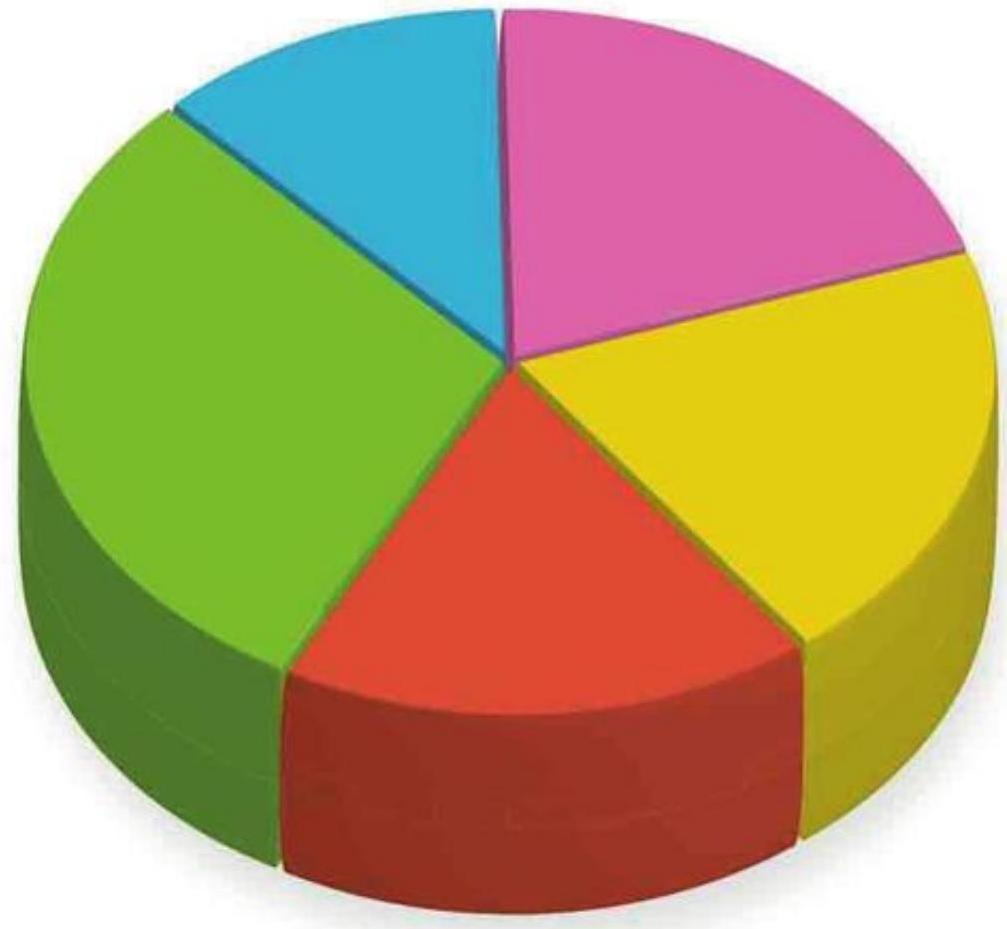
\includegraphics[max width=\textwidth, center]{2025_07_08_04014fa2c17a4b6cdcc6g-003}\\

\includegraphics[max width=\textwidth, center]{2025_07_08_04014fa2c17a4b6cdcc6g-005}

\section*{HELP YOUR KIDS WITH MathS A UNIQUE STEP-BY-STEP VISUAL GUIDE}
\section*{Project Art Editor}
Mark Lloyd

\section*{Designers}
Nicola Erdpresser, Riccie Janus, Maxine Pedliham, Silke Spingies, Rebecca Tennant

\section*{Design Assistants \\
 Thomas Howey, Fiona Macdonald}
\section*{Production Editor}
Luca Frassinetti

\section*{Jacket Designer}
Duncan Turner

\section*{Managing Art Editor}
Michelle Baxter

\section*{Art Director}
Phil Ormerod

\section*{Project Editor}
Nathan Joyce

\section*{Editors}
Nicola Deschamps, Martha Evatt,\\
Lizzie Munsey, Martyn Page, Laura Palosuo, Peter Preston, Miezan van Zyl

\section*{Indexer}
Jane Parker

\section*{Production}
Erica Pepe

\section*{Managing Editor}
Sarah Larter

\section*{Publishing Manager}
Liz Wheeler

\section*{Reference Publisher}
Jonathan Metcalf

First published in Great Britain in 2010 by Dorling Kindersley Limited 80 Strand, London WC2R ORL

A Penguin Random House Company\\
Copyright © 2010, 2014 Dorling Kindersley Limited

$$
\begin{gathered}
24681097531 \\
001-263995-J u l / 2014
\end{gathered}
$$

All rights reserved. No part of this publication may be reproduced, stored in a retrieval system, or transmitted in any form or by any means, electronic, mechanical, photocopying, recording, or otherwise, without prior written permission of the copyright owner.

A CIP catalogue record for this book is available from the British Library.

ISBN: 9781409355717

\footnotetext{Printed and bound by South China Printing Company, China
}See our complete catalogue at \href{http://www.dk.com}{www.dk.com}

CAROL VORDERMAN M.A.(Cantab), MBE is one of Britain's best loved TV presenters and is renowned for her skills in mathematics. She has hosted numerous shows from light entertainment with Carol Vorderman's Better Homes and The Pride of Britain Awards, to scientific programmes such as Tomorrow's World, on the BBC, ITV and Channel 4. Whether co-hosting Channel 4's Countdown for 26 years, becoming the second best-selling female non-fiction author of the noughties decade in the UK, advising Rt Hon David Cameron on the future of potential mathematics education in the UK, Carol has a passion and devotion to explaining mathematics in an exciting and easily understandable way. In 2010 she launched her own online maths school \href{http://www.themathsfactor.com}{www.themathsfactor.com} where she teaches parents and children how they can become the very best they can be in the art of arithmetic.

BARRY LEWIS (Consultant Editor, Numbers, Geometry, Trigonometry, Algebra) read mathematics at university and graduated with a first class honours degree. He spent many years in publishing, as an author and as an editor, where he developed a passion for mathematical books that presented this often difficult subject in accessible, appealing, and visual ways. Among these is Diversions in Modern Mathematics, which subsequently appeared in Spanish as Matemáticas modernas. Aspectos recreativos.

He was invited by the British Government to run the major initiative Maths Year 2000, a celebration of mathematical achievement with the aim of making the subject more popular and less feared. In 2001 Barry became the President of The Mathematical Association, and for his achievements in popularizing mathematics he was elected a Fellow of the Institute of Mathematics and its Applications. He is currently the Chair of Council of The Mathematical Association and regularly publishes articles and books dealing with both research topics and ways of engaging people in this critical subject.

ANDREW JEFFREY (Probability) is a maths consultant, well known for his passion and enthusiasm for the teaching and learning of mathematics. A teacher and inspector for over 20 years, Andrew now spends his time training, coaching, and supporting teachers and delivering lectures for various organizations throughout Europe. Andrew's previous books include Magic Maths for Kids, Top 20 Maths Displays, 100 Top Tips for Top Maths Teachers, and Be a Wizard With Numbers. Andrew is also better known to many schools as the Mathemagician, delivering his "Magic of Maths" shows to young and old! \href{http://www.andrewjeffrey.co.uk}{www.andrewjeffrey.co.uk}.

MARCUS WEEKS (Statistics) is the author of many books and has contributed to several encyclopedias, including DK's Science: The Definitive Visual Guide and Children's Illustrated Encyclopedia.

SEAN MCARDLE (Consultant) was a headteacher in two primary schools and has a Master of Philosophy degree in Educational Assessment. He has written or co-written more than 100 mathematical textbooks for children and assessment books for teachers.

\section*{Contents}
FOREWORD by Carol Vorderman ..... 8\\
INTRODUCTION by Barry Lewis ..... 10\\
1 NUMBERS\\
Introducing numbers ..... 14\\
Addition ..... 16\\
Subtraction ..... 17\\
Multiplication ..... 18\\
Division ..... 22\\
Prime numbers ..... 26\\
Units of measurement ..... 28\\
Telling the time ..... 30\\
Roman numerals ..... 33\\
Positive and negative numbers ..... 34\\
Powers and roots ..... 36\\
Surds ..... 40\\
Standard form ..... 42\\
Decimals ..... 44\\
Binary numbers ..... 46\\
Fractions ..... 48\\
Ratio and proportion ..... 56\\
Percentages ..... 60\\
Converting fractions, decimals, and percentages ..... 64\\
Mental maths ..... 66\\
Rounding off ..... 70\\
Using a calculator ..... 72\\
Personal finance ..... 74\\
Business finance ..... 76

\section*{2 GEOMETRY}
What is geometry? ..... 80\\
Tools in geometry ..... 82\\
Angles ..... 84\\
Straight lines ..... 86\\
Symmetry ..... 88\\
Coordinates ..... 90\\
Vectors ..... 94\\
Translations ..... 98\\
Rotations ..... 100\\
Reflections ..... 102\\
Enlargements ..... 104\\
Scale drawings ..... 106\\
Bearings ..... 108\\
Constructions ..... 110\\
Loci ..... 114\\
Triangles ..... 116\\
Constructing triangles ..... 118\\
Congruent triangles ..... 120\\
Area of a triangle ..... 122\\
Similar triangles ..... 125\\
Pythagoras' theorem ..... 128\\
Quadrilaterals ..... 130\\
Polygons ..... 134\\
Circles ..... 138\\
Circumference and diameter ..... 140\\
Area of a circle ..... 142\\
Angles in a circle ..... 144\\
Chords and cyclic quadrilaterals ..... 146\\
Tangents ..... 148\\
Arcs ..... 150\\
Sectors ..... 151\\
Solids ..... 152\\
Volumes ..... 154\\
Surface area of solids ..... 156\\
3 TRIGONOMETRY\\
What is trigonometry? ..... 160\\
Using formulas in trigonometry ..... 161\\
Finding missing sides ..... 162\\
Finding missing angles ..... 164\\
4 ALGEBRA\\
What is algebra? ..... 168\\
Sequences ..... 170\\
Working with expressions ..... 172\\
Expanding and factorizing expressions ..... 174\\
Quadratic expressions ..... 176\\
Formulas ..... 177\\
Solving equations ..... 180\\
Linear graphs ..... 182\\
Simultaneous equations ..... 186\\
Factorizing quadratic equations ..... 190\\
The quadratic formula ..... 192\\
Quadratic graphs ..... 194\\
Inequalities ..... 198\\
5 STATISTICS\\
What is statistics? ..... 202\\
Collecting and organizing data ..... 204\\
Bar charts ..... 206\\
Pie charts ..... 210\\
Line graphs ..... 212\\
Averages ..... 214\\
Moving averages ..... 218\\
Measuring spread ..... 220\\
Histograms ..... 224\\
Scatter diagrams ..... 226\\
6 PROBABILITY\\
What is probability? ..... 230\\
Expectation and reality ..... 232\\
Combined probabilities ..... 234\\
Dependent events ..... 236\\
Tree diagrams ..... 238\\
Reference section ..... 240\\
Glossary ..... 252\\
Index ..... 258\\
Acknowledgements ..... 264

\section*{Foreword}
\begin{center}
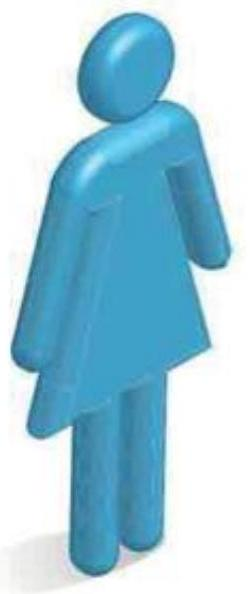
\includegraphics[max width=\textwidth]{2025_07_08_04014fa2c17a4b6cdcc6g-010(1)}
\end{center}

\section*{Hello}
Welcome to the wonderful world of maths. Research has shown just how important it is for a parent to be able to help a child with their education. Being able to work through homework together and enjoy a subject, particularly maths, is a vital part of a child's progress.

However, maths homework can be the cause of upset in many households. The introduction of new methods of arithmetic hasn't helped, as many parents are now simply unable to assist.

We wanted this book to guide parents through some of the methods in early arithmetic and then for them to go on to enjoy some deeper mathematics.

As a parent, I know just how important it is to be aware of when your child is struggling and equally, where they are shining. By having a greater understanding of maths, we can appreciate this even more.

Over nearly 30 years, and for nearly every single day, I have had the privilege of hearing people's very personal views about maths and arithmetic. Many weren't taught maths particularly well or in an interesting way. If you were one of those people, then we hope that this book can go some way to changing your situation and that maths, once understood, can begin to excite you as much as it does me.

\section*{CAROL VORDERMAN}

\includegraphics[max width=\textwidth, center]{2025_07_08_04014fa2c17a4b6cdcc6g-010}\\
$\boldsymbol{\Pi}=\mathbf{3 . 1 4 1 5 9 2 6 5 3 5 8 9 7 9 3 2 3 8 4 6 2 6 4 3 3 8 3 2}$ 7950288419716939937510582097494 4592307816406286208998628034853 4211706798214808651328230664709 3844609550582231725359408128481 11745028410270193852110555964462 2948954930381964428810975665933 4461284756482337867831652712019 0914564856692346034861045432664 8213393607260249141273724587006 6063155881748815209209628292540 91715364367892590360011330530548 8204665213841469519451160943305 72703657595919530921861173819326 11793105118548074462379962749567 3518857527248912279381830119491

\section*{Introduction}
\begin{center}
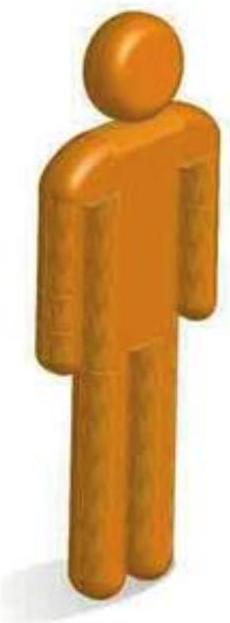
\includegraphics[max width=\textwidth]{2025_07_08_04014fa2c17a4b6cdcc6g-012}
\end{center}

This book concentrates on the mathematics tackled in schools between the ages of 9 and 16. But it does so in a gripping, engaging, and visual way. Its purpose is to teach maths by stealth. It presents mathematical ideas, techniques, and procedures so that they are immediately absorbed and understood. Every spread in the book is written and presented so that the reader will exclaim, "Ah ha - now I understand!". Pupils can use it on their own; equally, it helps a parent understand and remember the subject and so, help their child. If parents too gain something in the process, then so much the better.

At the start of the new millennium I had the privilege of being the Director of Maths Year 2000, a celebration of mathematics and an international effort to highlight and boost awareness of the subject. It was supported by the government and Carol Vorderman was also involved. Carol championed mathematics across the British media, but is well known for her astonishingly agile ways of manipulating and working with numbers - almost as if they were her personal friends. My working, domestic, and sleeping hours are devoted to mathematics - finding out how various subtle patterns based on counting items in sophisticated structures work and how they hang together. What united us was a shared passion for mathematics and the contribution it makes to all our lives - economic, cultural, and practical.

How is it that in a world ever more dominated by numbers, mathematics - the subtle art that teases out the patterns, the harmonies, and the textures that make\\
up the relationships between the numbers - is in danger ? I sometimes think that we are drowning in numbers.

As employees, our contribution is measured by targets, statistics, workforce percentages, and adherence to budget. As consumers, we are counted and aggregated according to every act of consumption. And in a nice subtlety, most of the products that we do consume come complete with their own personal statistics - the energy in the tin of beans and its lo (sic) salt content; the story in a newspaper and its swathe of statistics controlling and interpreting the world, developing each truth, simplifying each problem. Each minute of every hour; each hour of every day, we record and publish ever more readings from our collective life support machine. That is how we seek to understand the world, but the problem is, the more figures we get, the more truth seems to slip through our fingers.

The danger is, despite all the numbers and our increasingly numerate world, maths gets left behind. I'm sure that many think the ability to do the numbers is enough. Not so. Neither as individuals, nor collectively. Numbers are pinpricks in the fabric of mathematics, blazing within. Without them we would be condemned to total darkness. With them we gain glimpses of the sparkling treasures otherwise hidden.

This book sets out to address and solve this problem. Everyone can do maths.

\section*{BARRY LEWIS}
Former President, The Mathematical Association.\\
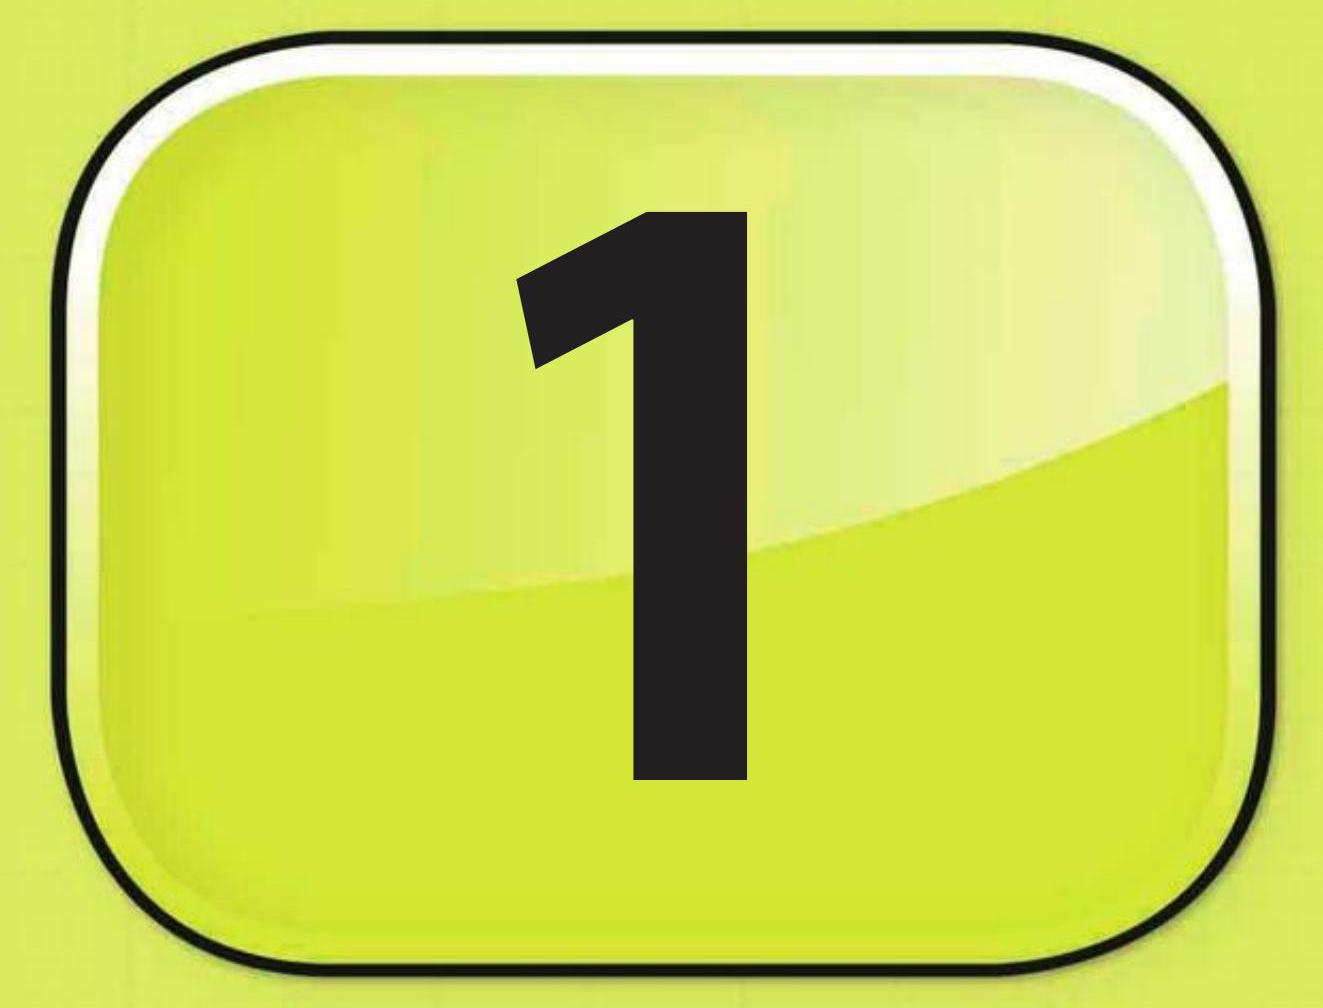
\includegraphics[max width=\textwidth, center]{2025_07_08_04014fa2c17a4b6cdcc6g-014}

Numbers

\section*{2 Introducing numbers}
\section*{COUNTING AND NUMBERS FORM THE FOUNDATION OF MATHEMATICS.}
Numbers are symbols that developed as a way to record amounts or quantities, but over centuries mathematicians have discovered ways to use and interpret numbers in order to work out new information.

\section*{What are numbers?}
Numbers are basically a set of standard symbols that represent quantities - the familiar 0 to 9. In addition to these whole numbers (also called integers) there are also fractions (see pp.48-55) and decimals (see pp.44-45). Numbers can also be negative, or less than zero (see pp.34-35).\\
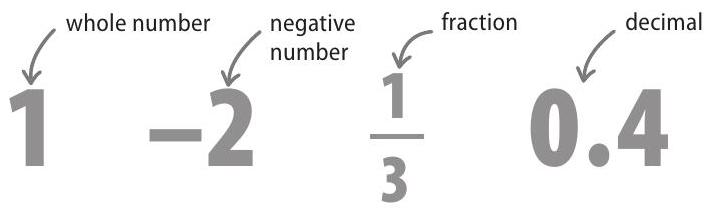
\includegraphics[max width=\textwidth, center]{2025_07_08_04014fa2c17a4b6cdcc6g-016}

\section*{$\triangle$ Types of numbers}
Here 1 is a positive whole number and -2 is a negative number. The symbol $1 / 3$ represents a fraction, which is one part of a whole that has been divided into three parts. A decimal is another way to express a fraction.

\begin{center}
\begin{tabular}{|l|}
\hline
LOOKING CLOSER \\
\hline
Zero \\
\hline
The use of the symbol for zero is considered an important advance in the way numbers are written. Before the symbol for zero was adopted, a blank space was used in calculations. This could lead to ambiguity and made numbers easier to confuse. For example, it was difficult to distinguish between 400, 40, and 4, since they were all represented by only the number 4. The symbol zero developed from a dot first used by Indian mathematicians to act a placeholder. \\
\hline
\end{tabular}
\end{center}

\begin{center}
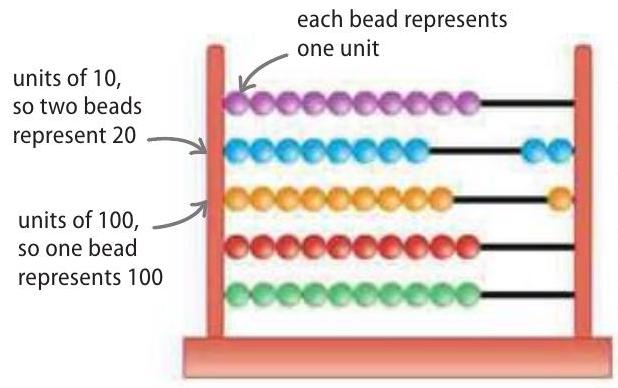
\includegraphics[max width=\textwidth]{2025_07_08_04014fa2c17a4b6cdcc6g-016(2)}
\end{center}

\section*{$\triangleleft$ Abacus}
The abacus is a traditional calculating and counting device with beads that represent numbers. The number shown here is 120.

\section*{$\nabla$ First number}
One is not a prime number. It is called the "multiplicative identity", because any number multiplied by 1 gives that number as the answer.\\
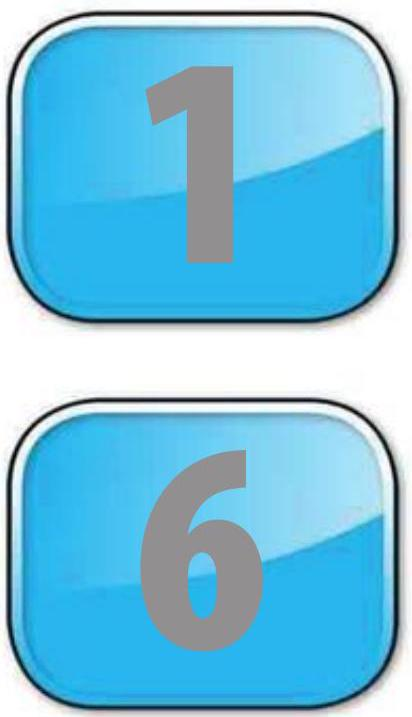
\includegraphics[max width=\textwidth, center]{2025_07_08_04014fa2c17a4b6cdcc6g-016(3)}

\section*{$\triangle$ Perfect number}
This is the smallest perfect number, which is a number that is the sum of its positive divisors (except itself). So, $1+2+3=6$.\\
$\nabla$ Even prime number\\
The number 2 is the only even-numbered prime number - a number that is only divisible by itself and 1 (see pp.26-27).\\
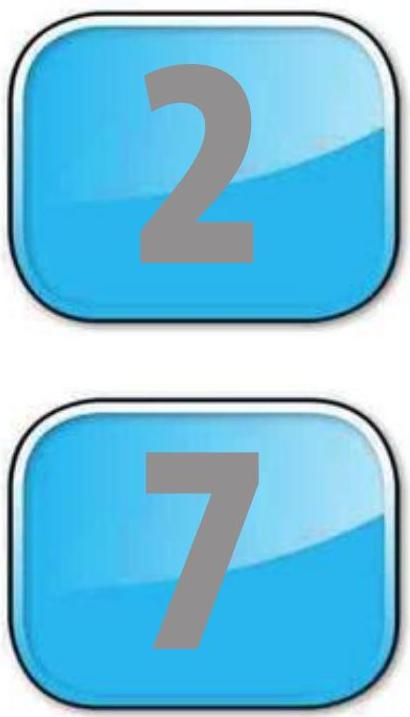
\includegraphics[max width=\textwidth, center]{2025_07_08_04014fa2c17a4b6cdcc6g-016(1)}\\
$\triangle$ Not the sum of squares\\
The number 7 is the lowest number that cannot be represented as the sum of the squares of three whole numbers (integers).

\section*{REAL WORLD}
\section*{Number symbols}
Many civilizations developed their own symbols for numbers，some of which are shown below，together with our modern Hindu－Arabic number system． One of the main advantages of our modern number system is that arithmetical operations，such as multiplication and division，are much easier to do than with the more complicated older number systems．

\begin{center}
\begin{tabular}{|l|l|l|l|l|l|l|l|l|l|l|}
\hline
Modern Hindu－Arabic & 1 & 2 & 3 & 4 & 5 & 6 & 7 & 8 & 9 & 10 \\
\hline
Mayan & $\bullet$ & $\bullet \bullet$ & $\bullet \bullet \bullet$ & $\bullet \bullet \bullet 0$ & － & $\bullet$ & $\bullet$ & $\bullet \bullet \bullet$ & $\bullet \bullet \bullet 0$ & ＝ \\
\hline
Ancient Chinese & 一 & 二 & 三 & 四 & 五 & 六 & 七 & 八 & 九 & 十 \\
\hline
Ancient Roman & I & II & III & IV & V & VI & VII & VIII & IX & X \\
\hline
Ancient Egyptian & 1 & ｜｜ & ｜｜｜ & II & III & III & IIII & IIII & III & ก \\
\hline
Babylonian & Y & T & m & 又 & 夜 & 登 & 登 & 器 & 枣 & ＜ \\
\hline
\end{tabular}
\end{center}

\section*{$\nabla$ Triangular number}
This is the smallest triangular number，which is a positive whole number that is the sum of consecutive whole numbers．So， $1+2=3$ ．\\
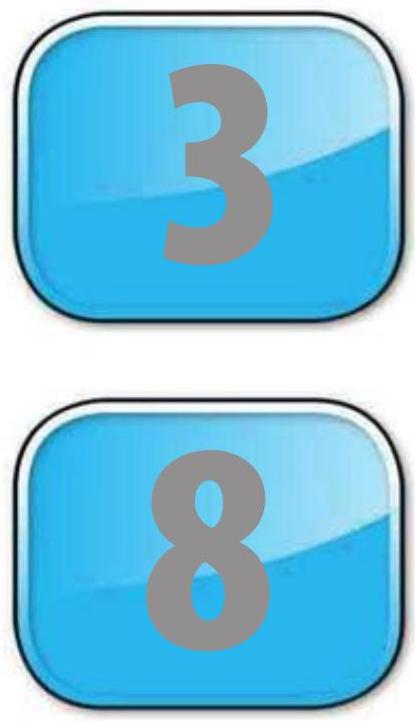
\includegraphics[max width=\textwidth, center]{2025_07_08_04014fa2c17a4b6cdcc6g-017(2)}

\section*{$\triangle$ Fibonacci number}
The number 8 is a cube number（ $2^{3}=8$ ）and it is the only positive Fibonacci number（see p．171），other than 1 ，that is a cube．

\section*{$\nabla$ Composite number}
The number 4 is the smallest composite number－a number that is the product of other numbers．The factors of 4 are two 2 s ．\\
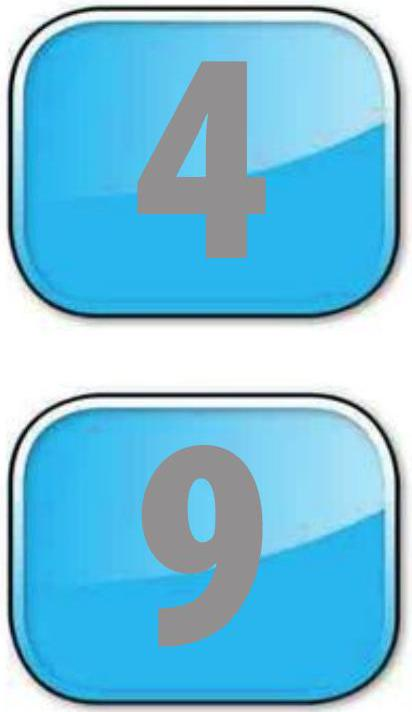
\includegraphics[max width=\textwidth, center]{2025_07_08_04014fa2c17a4b6cdcc6g-017}

\section*{Highest decimal}
The number 9 is the highest single－digit whole number and the highest single－digit number in the decimal system．

\section*{$\nabla$ Prime number}
This is the only prime number to end with a 5．A 5－sided polygon is the only shape for which the number of sides and diagonals are equal．\\
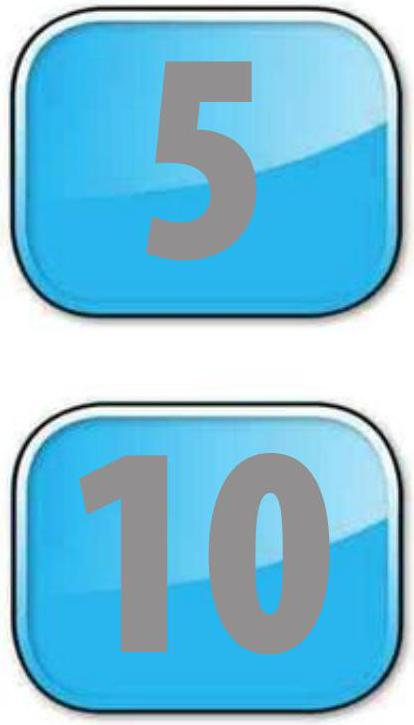
\includegraphics[max width=\textwidth, center]{2025_07_08_04014fa2c17a4b6cdcc6g-017(1)}

\section*{Base number}
The Western number system is based on the number 10. It is speculated that this is because humans used their fingers and toes for counting．

\section*{+ Addition}
\section*{NUMBERS ARE ADDED TOGETHER TO FIND THEIR TOTAL. THIS RESULT IS CALLED THE SUM.}
\section*{Adding up}
An easy way to work out the sum of two numbers is a number line. It is a group of numbers arranged in a straight line that makes it possible to count up or down.

\section*{SEE ALSO}
Subtraction\\
Positive and negative numbers

34-35 〉 In this number line, 3 is added to 1 .

\section*{What it means}
The result of adding 3 to the start number of 1 is 4. This means that the sum of 1 and 3 is 4 .\\
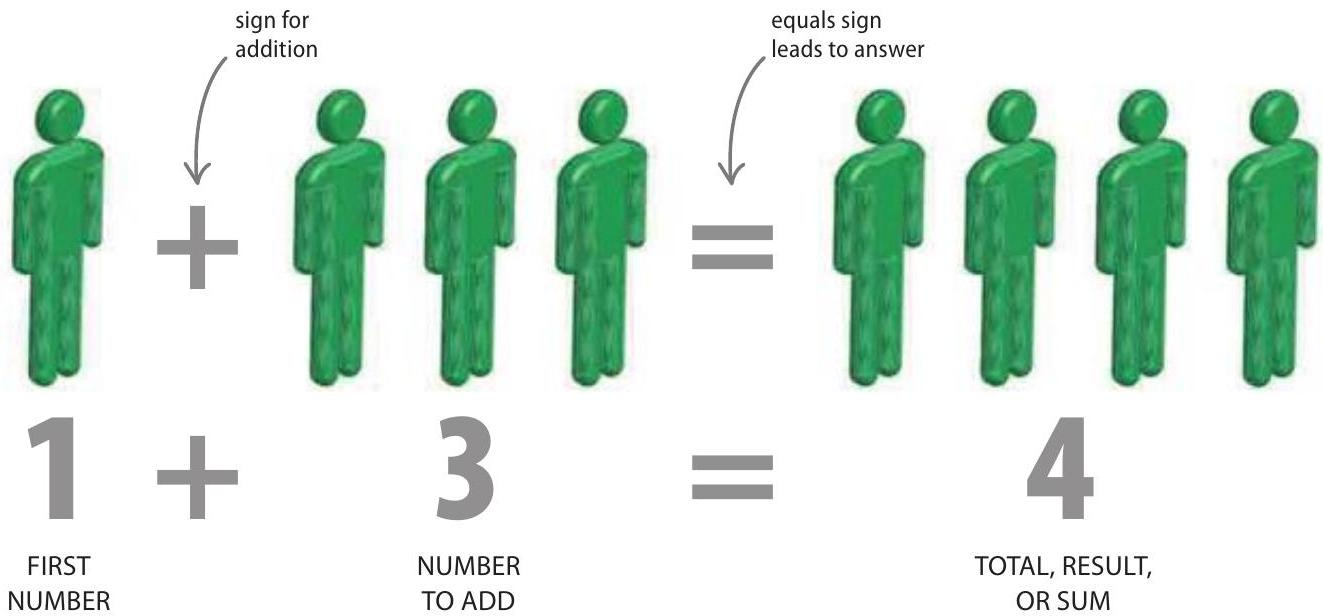
\includegraphics[max width=\textwidth, center]{2025_07_08_04014fa2c17a4b6cdcc6g-018}

\section*{Adding large numbers}
Numbers that have two or more digits are added in vertical columns. First, add the units, then the tens, the hundreds, and so on. The sum of each column is written beneath it. If the sum has two digits, the first is carried to the next column.\\
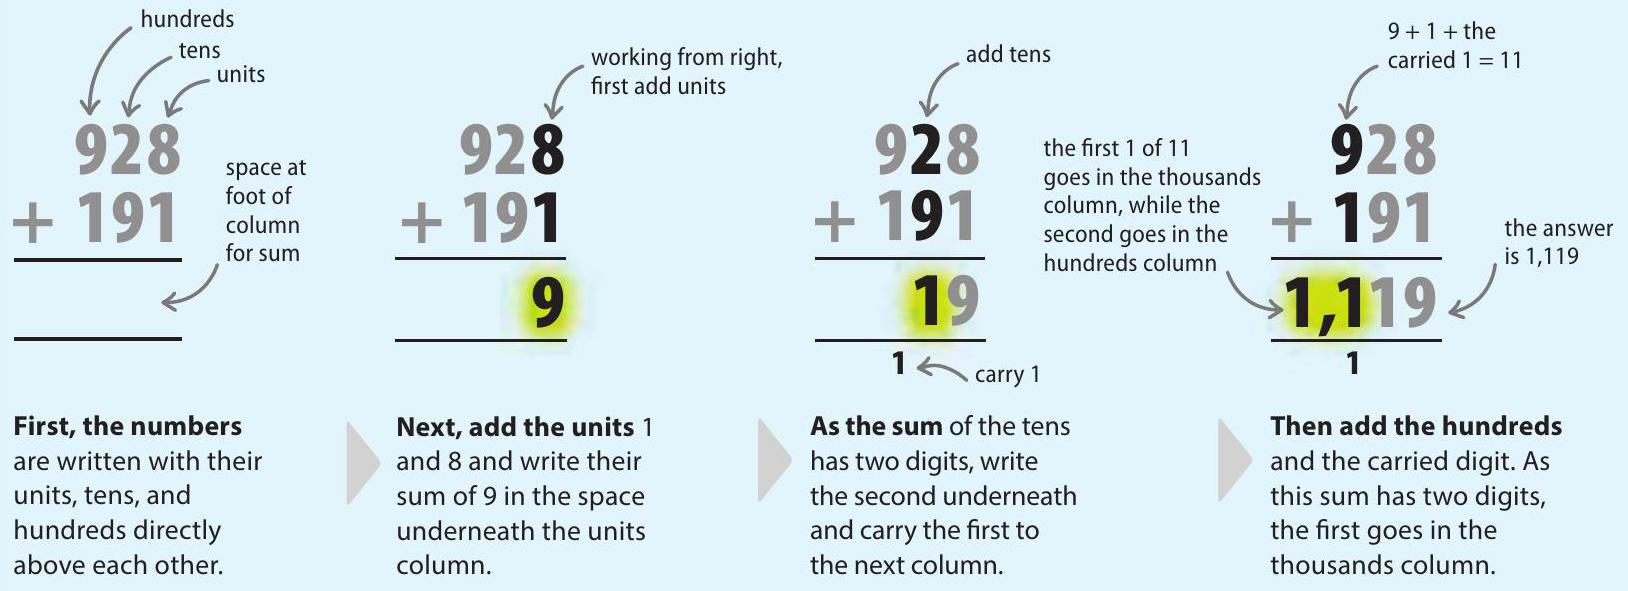
\includegraphics[max width=\textwidth, center]{2025_07_08_04014fa2c17a4b6cdcc6g-018(1)}

\section*{Subtraction}
\section*{A NUMBER IS SUBTRACTED FROM ANOTHER NUMBER TO FIND WHAT IS LEFT. THIS IS KNOWN AS THE DIFFERENCE.}
\section*{SEE ALSO}
《 16 Addition\\
Positive and negative numbers

34-35 〉

\section*{Taking away}
A number line can also be used to show how to subtract numbers. From the first number, move back along the line the number of places shown by the

Use a number line To subtract 3 from 4, start at 4 and move three places along the number line, first to 3 , second number. Here 3 is taken from 4.\\
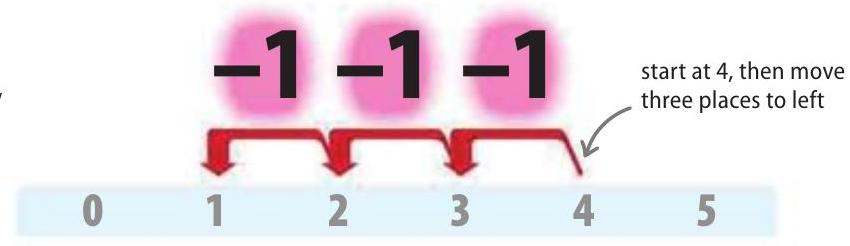
\includegraphics[max width=\textwidth]{2025_07_08_04014fa2c17a4b6cdcc6g-019(5)} then 2 , and then to 1 .\\
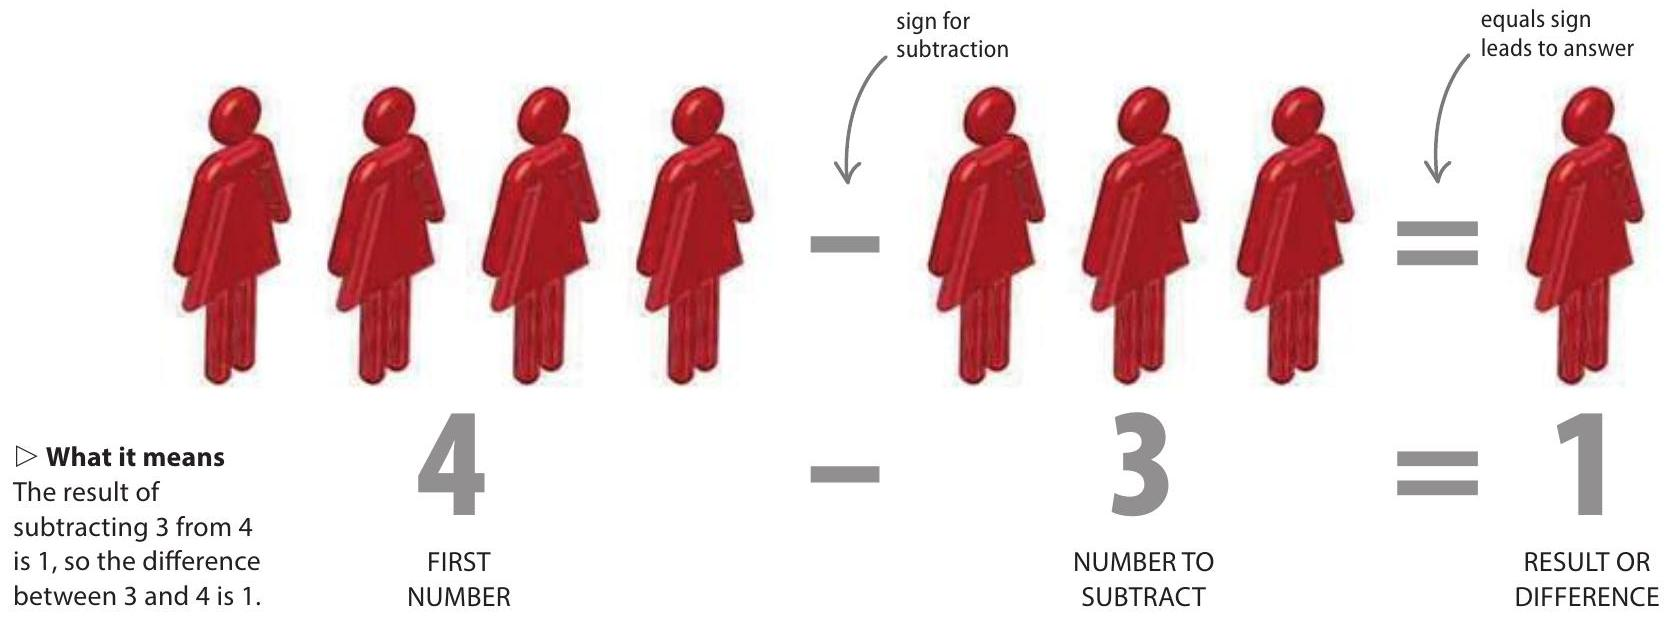
\includegraphics[max width=\textwidth, center]{2025_07_08_04014fa2c17a4b6cdcc6g-019(4)}

\section*{Subtracting large numbers}
Subtracting numbers of two or more digits is done in vertical columns. First subtract the units, then the tens, the hundreds, and so on. Sometimes a digit is borrowed from the next column along.\\
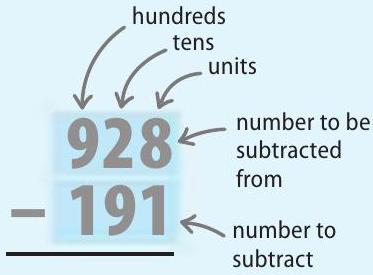
\includegraphics[max width=\textwidth, center]{2025_07_08_04014fa2c17a4b6cdcc6g-019(1)}

First, the numbers are written with their units, tens, and hundreds directly above each other.\\
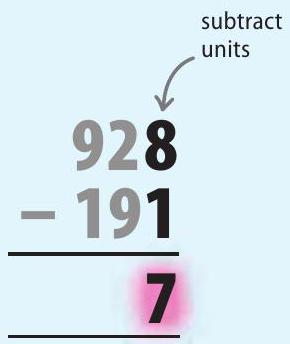
\includegraphics[max width=\textwidth, center]{2025_07_08_04014fa2c17a4b6cdcc6g-019}

Next, subtract the unit 1 from 8, and write their difference of 7 in the space underneath them.\\
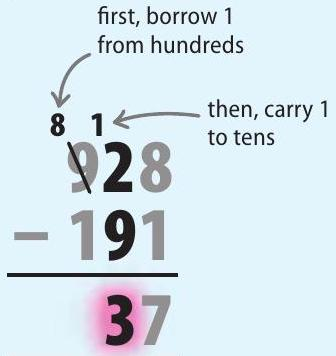
\includegraphics[max width=\textwidth, center]{2025_07_08_04014fa2c17a4b6cdcc6g-019(3)}

In the tens, 9 cannot be subtracted from 2, so 1 is borrowed from the hundreds, turning 9 into 8 and 2 into 12.\\
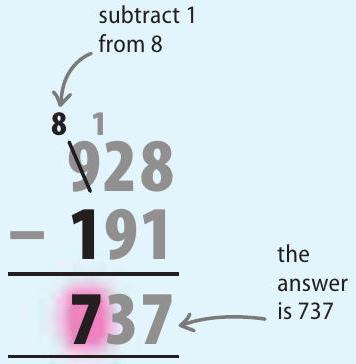
\includegraphics[max width=\textwidth, center]{2025_07_08_04014fa2c17a4b6cdcc6g-019(2)}

In the hundreds column, 1 is subtracted from the new, now lower number of 8 .

\section*{× Multiplication}
\section*{MULTIPLICATION INVOLVES ADDING A NUMBER TO ITSELF A NUMBER OF TIMES. THE RESULT OF MULTIPLYING NUMBERS IS CALLED THE PRODUCT.}
\section*{SEE ALSO}
《 16-17 Addition and Subtraction

\begin{center}
\begin{tabular}{ll}
\hline
Division & 22-25 $\boldsymbol{>}$ \\
\hline
Decimals & $\mathbf{4 4 - 4 5} \boldsymbol{>}$ \\
\hline
\end{tabular}
\end{center}

\section*{What is multiplication?}
The second number in a multiplication sum is the number to be added to itself and the first is the number of times to add it. Here the number of rows of people is added together a number of times determined by the number of people in each row. This multiplication sum gives the total number of people in the group.

\section*{Works both ways}
It does not matter which order numbers appear in a multiplication sum because the answer will be the same either way. Two methods of the same multiplication are shown here.\\
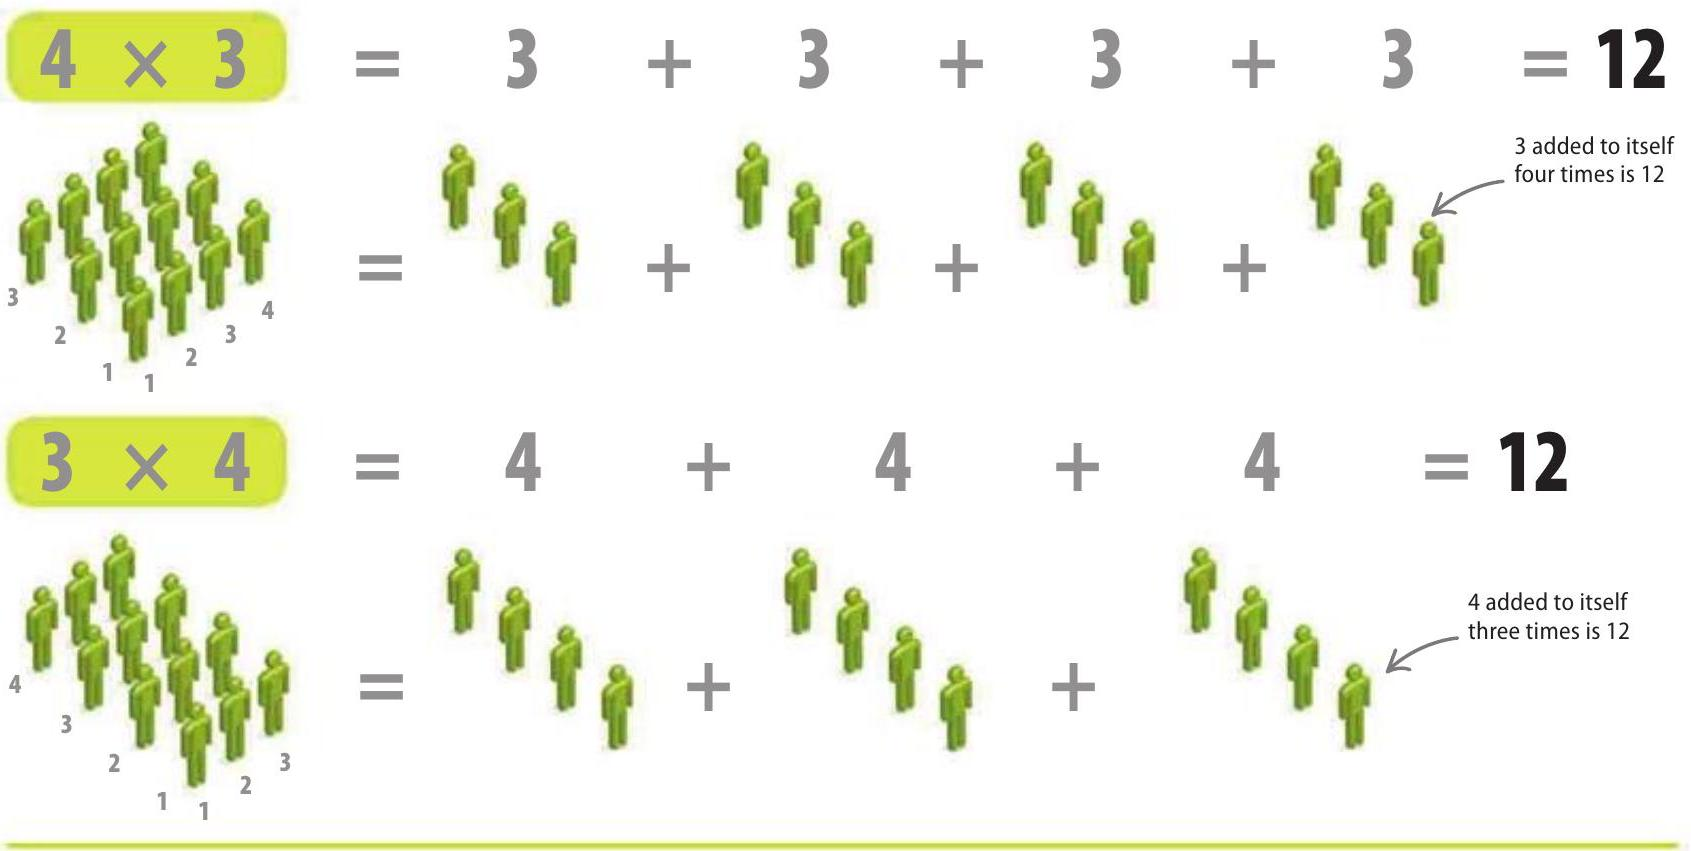
\includegraphics[max width=\textwidth, center]{2025_07_08_04014fa2c17a4b6cdcc6g-021(1)}

Multiplying by 10, 100, 1,000\\
Multiplying whole numbers by 10, 100, 1,000, and so on involves adding one zero (0), two zeroes (00), three zeroes (000), and so on to the right of the start number.\\
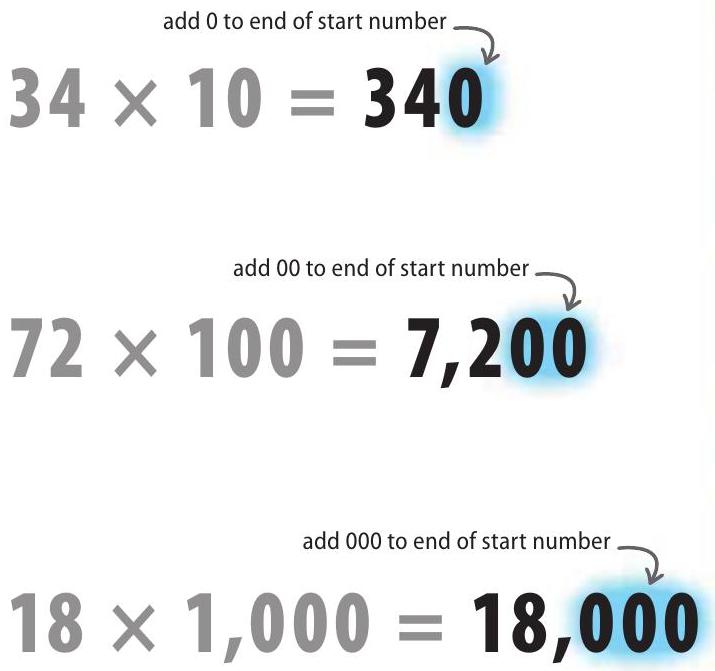
\includegraphics[max width=\textwidth, center]{2025_07_08_04014fa2c17a4b6cdcc6g-021}

\section*{Patterns of multiplication}
There are quick ways to multiply two numbers, and these patterns of multiplication are easy to remember. The table shows patterns involved in multiplying numbers by $2,5,6,9,12$, and 20 .

\begin{center}
\begin{tabular}{|l|l|l|}
\hline
\multicolumn{3}{|c|}{PATTERNS OF MULTIPLICATION} \\
\hline
To multiply & How to do it & Example to multiply \\
\hline
2 & add the number to itself & $2 \times 11=11+11=22$ \\
\hline
5 & the last digit of the number follows the pattern 5, 0, 5, 0 & 5, 10, 15, 20 \\
\hline
6 & multiplying 6 by any even number gives an answer that ends in the same last digit as the even number & \begin{tabular}{l}
$6 \times 12=72$ \\
$6 \times 8=48$ \\
\end{tabular} \\
\hline
9 & multiply the number by 10 , then subtract the number & $9 \times 7=10 \times 7-7=63$ \\
\hline
12 & multiply the original number first by 10 , then multiply the original number by 2 , and then add the two answers & \begin{tabular}{l}
$12 \times 10=120$ \\
$12 \times 2=24$ \\
$120+24=144$ \\
\end{tabular} \\
\hline
20 & multiply the number by 10 then multiply the answer by 2 & \begin{tabular}{l}
$14 \times 20=$ \\
$14 \times 10=140$ \\
$140 \times 2=280$ \\
\end{tabular} \\
\hline
\end{tabular}
\end{center}

\section*{MULTIPLES}
When a number is multiplied by any whole number the result (product) is called a multiple. For example, the first six multiples of the number 2 are $2,4,6,8,10$, and 12 . This is because $2 \times 1=2,2 \times 2=4,2 \times 3=6,2 \times 4=8,2 \times 5=10$, and $2 \times 6=12$.\\
MULTIPLES OF 3\\
$3 \times 1=\mathbf{3}$\\
$3 \times \mathbf{2}=\mathbf{6}$\\
$3 \times 3=\mathbf{9}$\\
$3 \times \mathbf{4}=\mathbf{1 2}$\\
$3 \times 5=\mathbf{1 5}$\\
MULTIPLES OF 8\\
$8 \times 1=8$\\
$8 \times 2=16$\\
$8 \times 3=24$\\
$8 \times 4=32$\\
$8 \times 5=40$\\
MULTIPLES OF 12\\
$12 \times 1=12$\\
$12 \times 2=24$\\
$12 \times 3=36$\\
$12 \times 4=48$\\
$12 \times 5=60$

\section*{Common multiples}
Two or more numbers can have multiples in common. Drawing a grid, such as the one on the right, can help find the common multiples of different numbers. The smallest of these common numbers is called the lowest common multiple.\\
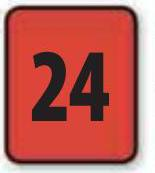
\includegraphics[max width=\textwidth, center]{2025_07_08_04014fa2c17a4b6cdcc6g-022}\\
owest common multiple The lowest common multiple of 3 and 8 is 24 because it is the smallest number that both multiply into\\

\includegraphics[max width=\textwidth, center]{2025_07_08_04014fa2c17a4b6cdcc6g-022(1)}\\
multiples of 3\\
multiples of 8\\
multiples of 3 and 8

\section*{- Finding common multiples}
Multiples of 3 and multiples of 8 are highlighted on this grid. Some multiples are common to both numbers.

\begin{center}
\begin{tabular}{|l|l|l|l|l|l|l|l|l|l|}
\hline
1 & 2 & 3 & 4 & 5 & 6 & 7 & 8 & 9 & 10 \\
\hline
11 & 12 & 13 & 14 & 15 & 16 & 17 & 18 & 19 & 20 \\
\hline
21 & 22 & 23 & 24 & 25 & 26 & 27 & 28 & 29 & 30 \\
\hline
31 & 32 & 33 & 34 & 35 & 36 & 37 & 38 & 39 & 40 \\
\hline
41 & 42 & 43 & 44 & 45 & 46 & 47 & 48 & 49 & 50 \\
\hline
51 & 52 & 53 & 54 & 55 & 56 & 57 & 58 & 59 & 60 \\
\hline
61 & 62 & 63 & 64 & 65 & 66 & 67 & 68 & 69 & 70 \\
\hline
71 & 72 & 73 & 74 & 75 & 76 & 77 & 78 & 79 & 80 \\
\hline
81 & 82 & 83 & 84 & 85 & 86 & 87 & 88 & 89 & 90 \\
\hline
91 & 92 & 93 & 94 & 95 & 96 & 97 & 98 & 99 & 100 \\
\hline
\end{tabular}
\end{center}

\section*{Short multiplication}
Multiplying a large number by a single-digit number is called short multiplication. The smaller number is placed below the larger one and aligned under the units column of the larger number.\\
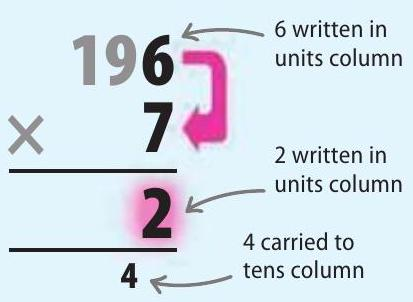
\includegraphics[max width=\textwidth, center]{2025_07_08_04014fa2c17a4b6cdcc6g-023(3)}

To multiply 196 and 7, first multiply the units 7 and 6. The product is 42 , the 4 of which is carried.\\
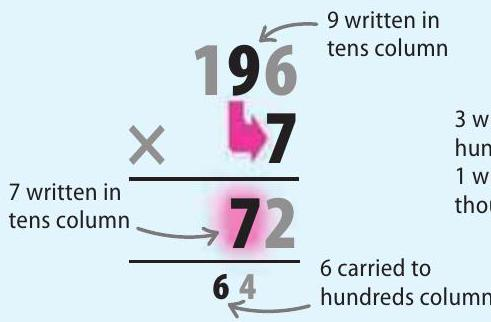
\includegraphics[max width=\textwidth, center]{2025_07_08_04014fa2c17a4b6cdcc6g-023(1)}

Next, multiply 7 and 9, the product of which is 63. The carried 4 is added to 63 to get 67 .\\
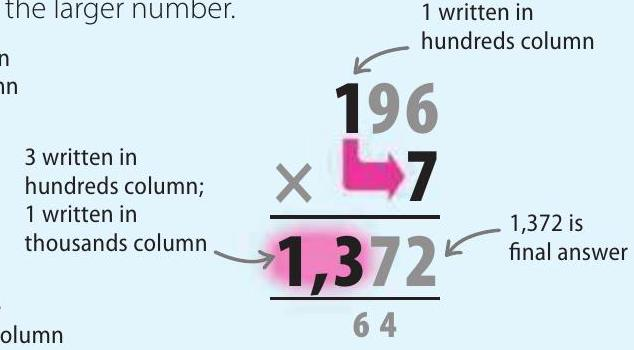
\includegraphics[max width=\textwidth, center]{2025_07_08_04014fa2c17a4b6cdcc6g-023(4)}

Finally, multiply 7 and 1. Add the product (7) to the carried 6 to get 13, giving a final product of 1,372.

\section*{Long multiplication}
Multiplying two numbers that both contain at least two digits is called long multiplication. The numbers are placed one above the other, in columns arranged according to their value (units, tens, hundreds, and so on).\\
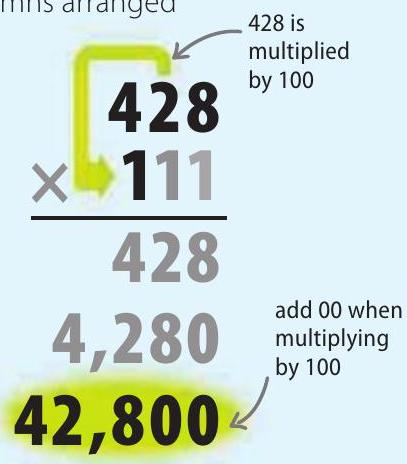
\includegraphics[max width=\textwidth, center]{2025_07_08_04014fa2c17a4b6cdcc6g-023(2)}

Multiply 428 by 1 in the hundreds column, digit by digit. Add 00 to the product when multiplying by 100.\\
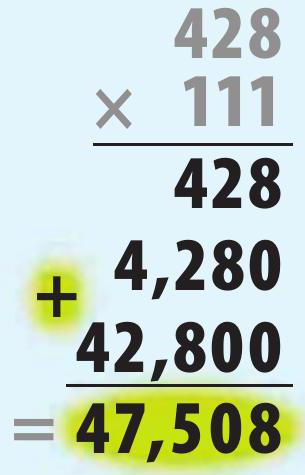
\includegraphics[max width=\textwidth, center]{2025_07_08_04014fa2c17a4b6cdcc6g-023}

Add together the products of the three multiplications. The answer is 47,508.

Multiply 428 by 1 in the tens column, working digit by digit. Remember to add 0 to the product when multiplying by 10 .\\
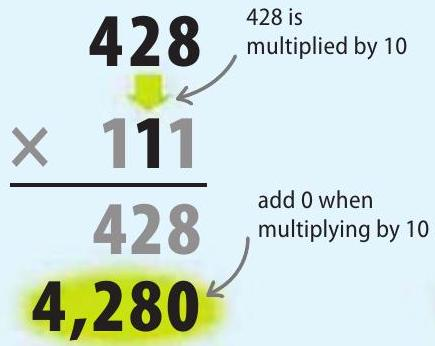
\includegraphics[max width=\textwidth, center]{2025_07_08_04014fa2c17a4b6cdcc6g-023(6)}

First, multiply 428 by 1 in the units column. Work digit by digit from right to left so $8 \times 1,2 \times 1$, and then $4 \times 1$.\\
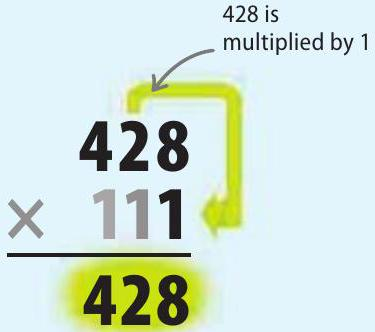
\includegraphics[max width=\textwidth, center]{2025_07_08_04014fa2c17a4b6cdcc6g-023(5)}

OOKING CLOSER

\section*{Box method of multiplication}
The long multiplication of 428 and 111 can be broken down into simple multiplications with the help of a table or a box. Each number is reduced to its hundreds, tens, and units, and multiplied by the other.

\section*{$\triangleright$ The final step}
Add together the nine multiplications to find the final answer.

\begin{center}
\begin{tabular}{|l|l|l|l|l|l|l|}
\hline
 & \multicolumn{4}{|c|}{428 WRITTEN IN 100S, 10S, AND UNITS} & \multirow{2}{*}{40,000 2,000 800} & \multirow{9}{*}{this is the final answer} \\
\hline
\multirow{8}{*}{111 WRITTEN IN 100S, 10S, AND UNITS} & \multicolumn{4}{|c|}{20} &  &  \\
\hline
 &  &  &  &  & \multirow{3}{*}{4,000 200 80} &  \\
\hline
 & 100 & $400 \times 100$ $=40,000$ & $20 \times 100$ =2,000 & $8 \times 100$ $=800$ &  &  \\
\hline
 &  &  &  &  & \multicolumn{2}{|l|}{\multirow[b]{5}{*}}{} \\
\hline
 & 10 & $400 \times 10$ $=4,000$ & $20 \times 10$ $=200$ & $8 \times 10$ $=80$ &  &  \\
\hline
 &  &  &  &  &  &  \\
\hline
 &  &  &  &  &  &  \\
\hline
 & 1 & $400 \times 1$ $=400$ & $20 \times 1$ $=20$ & $8 \times 1$ $=8$ &  &  \\
\hline
\end{tabular}
\end{center}

\section*{Division}
\section*{DIVISION INVOLVES FINDING OUT HOW MANY TIMES ONE NUMBER GOES INTO ANOTHER NUMBER.}
\begin{center}
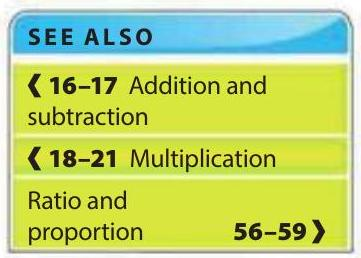
\includegraphics[max width=\textwidth]{2025_07_08_04014fa2c17a4b6cdcc6g-024}
\end{center}

There are two ways to think about division. The first is sharing a number out equally ( 10 coins to 2 people is 5 each). The other is dividing a number into equal groups ( 10 coins into piles containing 2 coins each is 5 piles).

\section*{How division works}
Dividing one number by another finds out how many times the second number (the divisor) fits into the first (the dividend). For example, dividing 10 by 2 finds out how many times 2 fits into 10. The result of the division is known as the quotient.\\
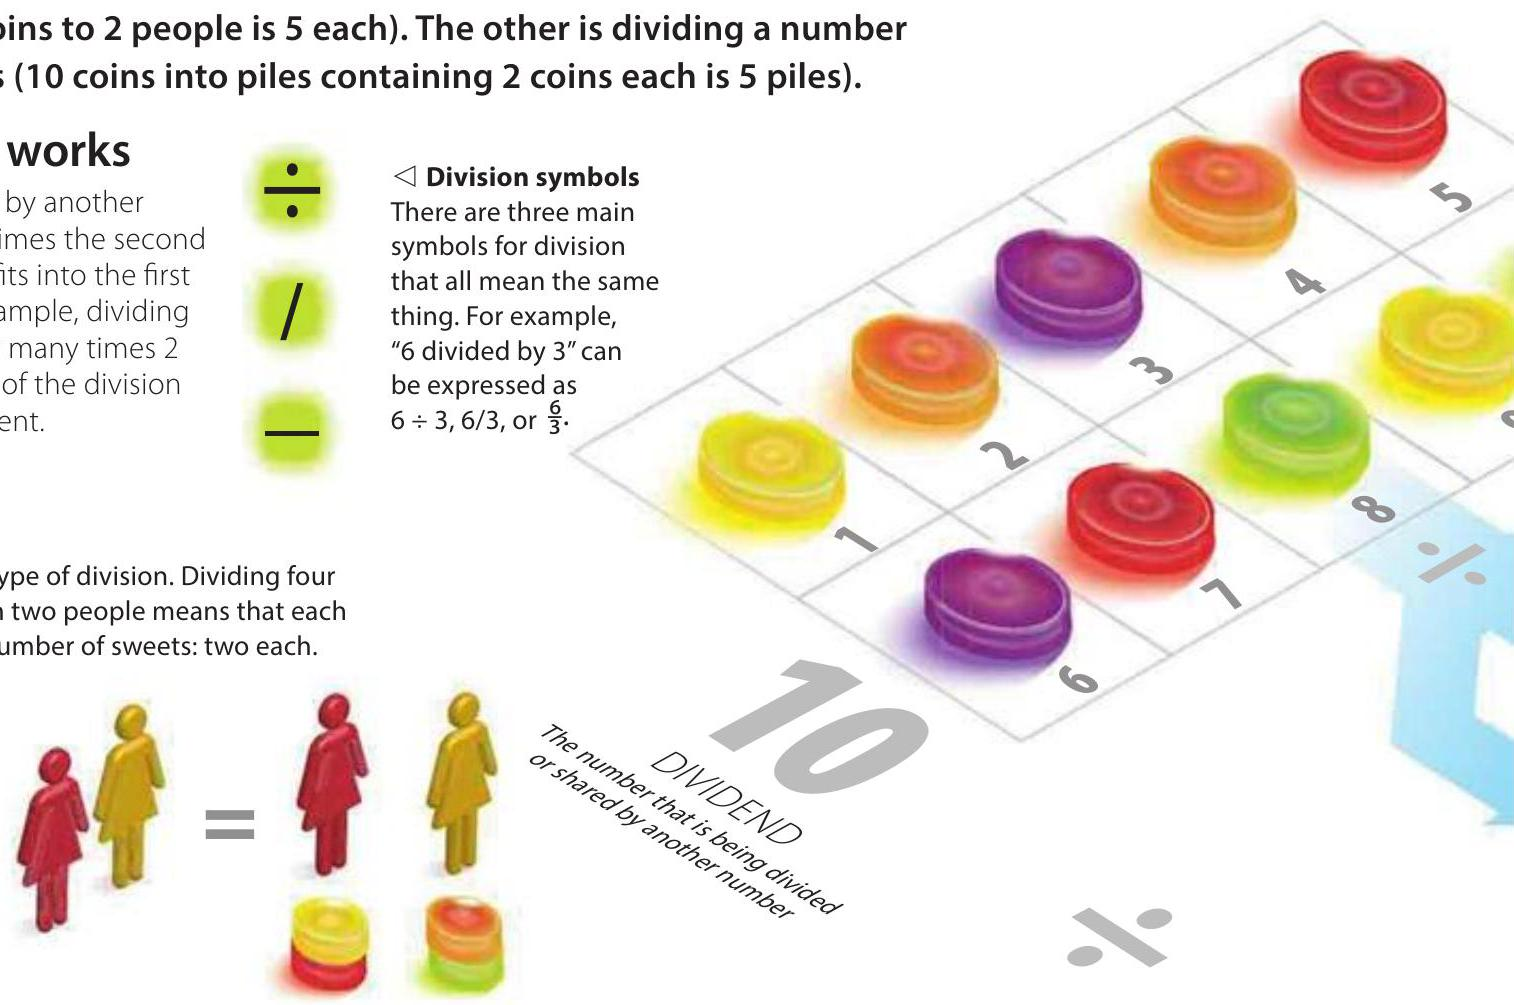
\includegraphics[max width=\textwidth, center]{2025_07_08_04014fa2c17a4b6cdcc6g-024(1)}

\section*{$\nabla$ Division as sharing}
Sharing equally is one type of division. Dividing four sweets equally between two people means that each person gets the same number of sweets: two each.

\section*{$\mathbf{4}_{\text {sweets }} \div \mathbf{2}_{\text {people }}=\mathbf{2}_{\text {swets per person }}$}
\section*{LOOKING CLOSER}
\section*{How division is linked to multiplication}
Division is the direct opposite or "inverse" of multiplication, and the two are always connected. If you know the answer to a particular division, you can form a multiplication from it and vice versa.

\section*{$\triangleleft$ Back to the beginning}
If 10 (the dividend) is divided by 2 (the divisor), the answer (the quotient) is 5 . Multiplying the quotient (5) by the divisor of the original division sum (2) results in the original dividend (10).

$$
10 \div 2=5 \quad 5 \times 2=10
$$

\section*{Another approach to division}
Instead of thinking of it as sharing out a number, division can also be viewed as finding out how many groups of the second number (divisor) are contained in the first number (dividend). The division sum remains the same in both sharing and grouping.

\section*{$\nabla$ Introducing remainders}
In this example, 10 sweets are being divided between 3 girls. However, 3 does not divide exactly into 10 - it fits 3 times with 1 left over. The amount left over from a division sum is called the remainder.

This example shows 30 footballs, which are to be divided into\\
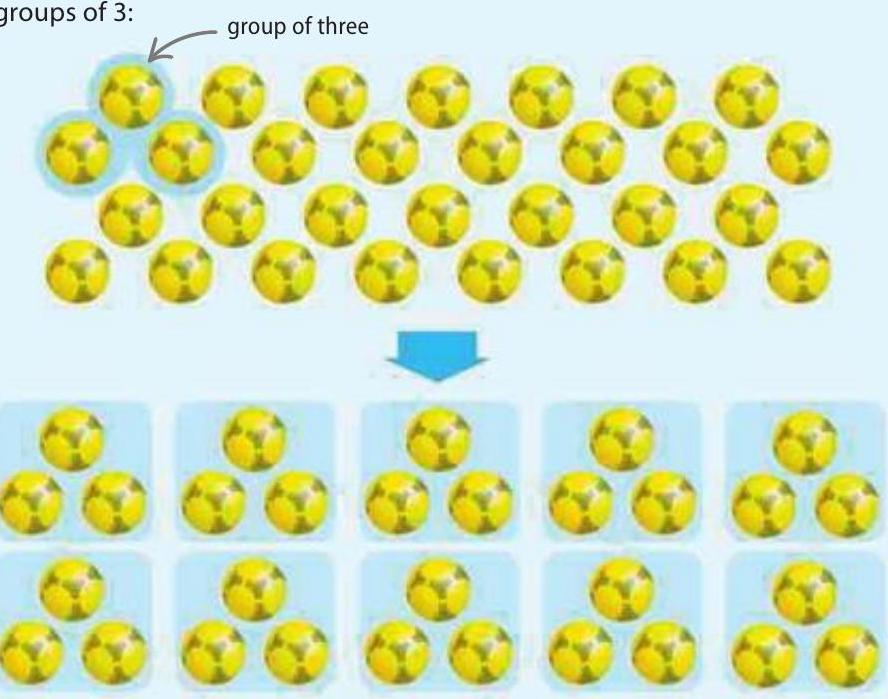
\includegraphics[max width=\textwidth, center]{2025_07_08_04014fa2c17a4b6cdcc6g-025}

There are exactly 10 groups of 3 footballs, with no remainder, so $30 \div 3=\mathbf{1 0}$.

\begin{center}
\begin{tabular}{|l|l|l|}
\hline
\multicolumn{3}{|c|}{DIVISION TIPS} \\
\hline
A number is divisible by & If... & Examples \\
\hline
2 & the last digit is an even number & 12, 134, 5,000 \\
\hline
3 & the sum of all digits when added together is divisible by 3 & 18 $1+8=9$ \\
\hline
4 & the number formed by the last two digits is divisible by 4 & 732 $32 \div 4=8$ \\
\hline
5 & the last digit is 5 or 0 & 25, 90, 835 \\
\hline
6 & the last digit is even and the sum of its digits when added together is divisible by 3 & 3,426 $3+4+2+6=15$ \\
\hline
7 & no simple divisibility test &  \\
\hline
8 & the number formed by the last three digits is divisible by 8 & 7,536 $536 \div 8=67$ \\
\hline
9 & the sum of all of its digits is divisible by 9 & 6,831 $6+8+3+1=18$ \\
\hline
10 & the number ends in 0 & 30, 150, 4,270 \\
\hline
\end{tabular}
\end{center}

\section*{Short division}
Short division is used to divide one number (the dividend) by another whole number (the divisor) that is less than 10.\\
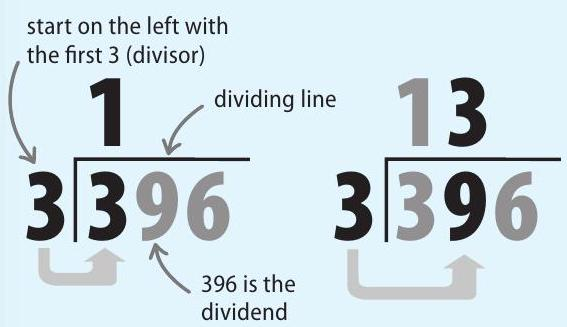
\includegraphics[max width=\textwidth, center]{2025_07_08_04014fa2c17a4b6cdcc6g-026(5)}

Divide the first 3 into 3. It fits once exactly, so put a 1 above the dividing line, directly above the 3 of the dividend.

Move to the next column and divide 3 into 9. It fits three times exactly, so put a 3 directly above the 9 of the dividend.\\
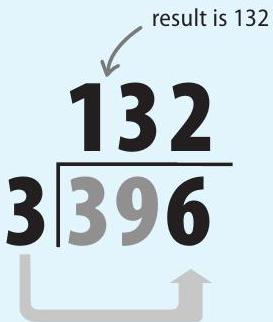
\includegraphics[max width=\textwidth, center]{2025_07_08_04014fa2c17a4b6cdcc6g-026(9)}

Divide 3 into 6, the last digit of the dividend. It goes twice exactly, so put a 2 directly above the 6 of the dividend.

\section*{Carrying numbers}
When the result of a division gives a whole number and a remainder, the remainder can be carried over to the next digit of the dividend.\\
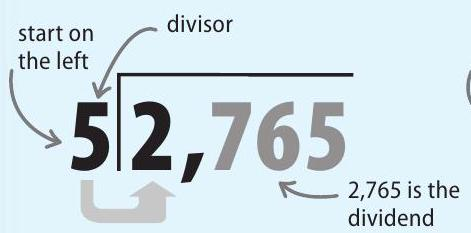
\includegraphics[max width=\textwidth, center]{2025_07_08_04014fa2c17a4b6cdcc6g-026(7)}\\
divide 5 int first 2 digits of dividend\\
carry remainder 2 to next digit\\
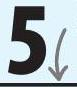
\includegraphics[max width=\textwidth]{2025_07_08_04014fa2c17a4b6cdcc6g-026(2)} of dividend

Start with number 5. It does not divide into 2 as it is a larger number. Instead, 5 will need to be divided into the first two digits of the dividend.\\
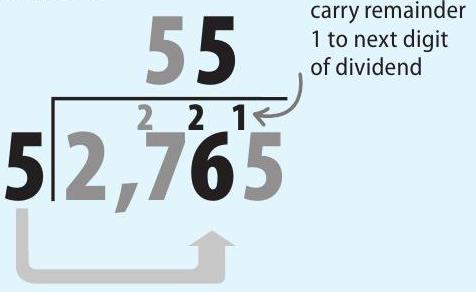
\includegraphics[max width=\textwidth, center]{2025_07_08_04014fa2c17a4b6cdcc6g-026(1)}

Divide 5 into 26. The result is 5 with a remainder of 1 . Put 5 directly above the 6 and carry the remainder 1 to the next digit of the dividend.

Divide 5 into 27. The result is 5 with a remainder of 2 . Put 5 directly above the 7 and carry the remainder.\\
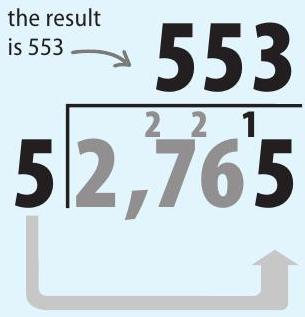
\includegraphics[max width=\textwidth, center]{2025_07_08_04014fa2c17a4b6cdcc6g-026(3)}

Divide 5 into 15. It fits three times exactly, so put 3 above the dividing line, directly above the final 5 of the dividend.

\section*{22.5 $4 \longdiv { 9 0 . 0 }$ \\
 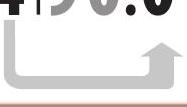
\includegraphics[max width=\textwidth]{2025_07_08_04014fa2c17a4b6cdcc6g-026}}
Remove the remainder, 2 in this case, leaving 22. Add a decimal point above and below the dividing line. Next, add a zero to the dividend after the decimal point.

\section*{22.}
Carry the remainder (2) from above the dividing line to below the line and put it in front of the new zero.

Divide 4 into 20. It goes 5 times exactly, so put a 5 directly above the zero of the dividend and after the decimal point.

\section*{LOOKING CLOSER}
\section*{Making division simpler}
To make a division easier, sometimes the divisor can be split into factors. This means that a number of simpler divisions can be done.

\section*{LOOKING CLOSER}
\section*{Converting remainders}
When one number will not divide exactly into another, the answer has a remainder. Remainders can be converted into decimals, as\\
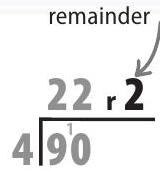
\includegraphics[max width=\textwidth]{2025_07_08_04014fa2c17a4b6cdcc6g-026(4)} shown below.\\
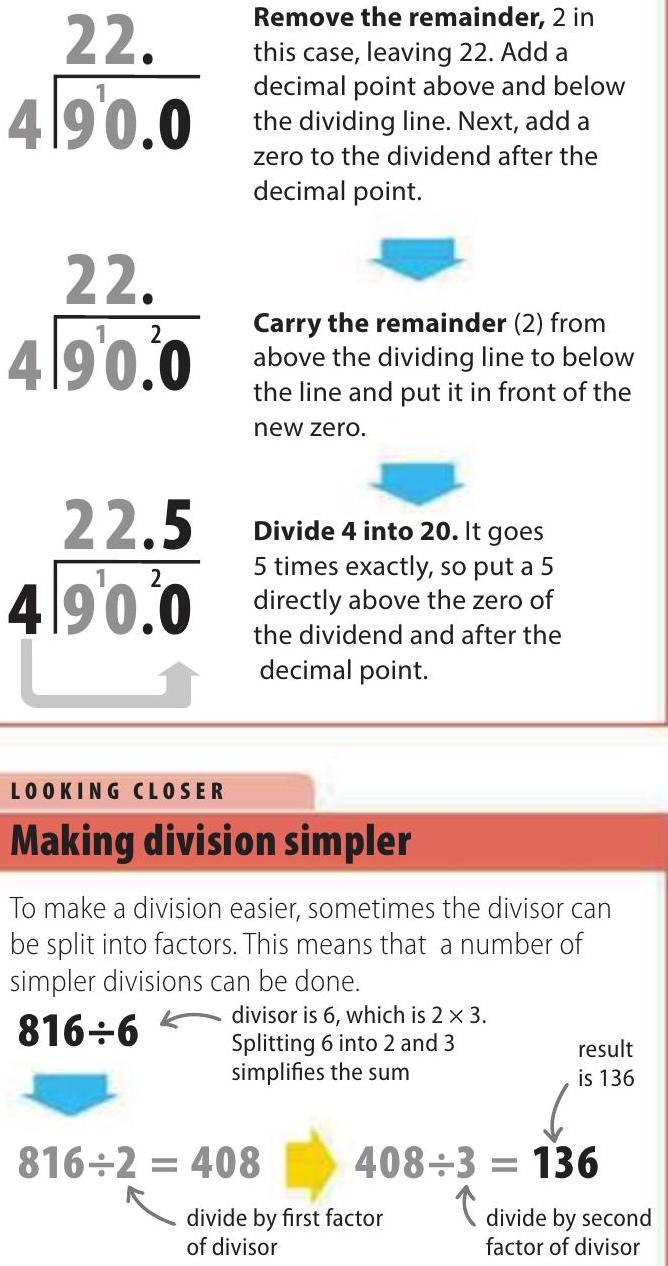
\includegraphics[max width=\textwidth, center]{2025_07_08_04014fa2c17a4b6cdcc6g-026(8)}

This method of splitting the divisor into factors can also be used for more difficult divisions.\\
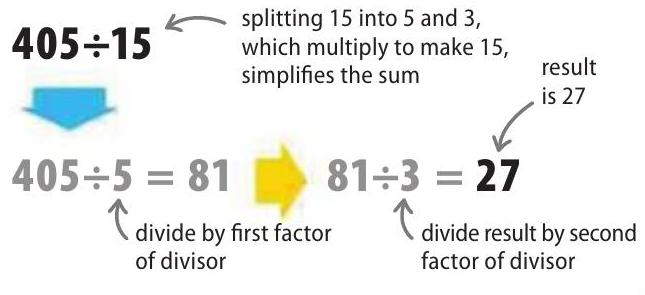
\includegraphics[max width=\textwidth, center]{2025_07_08_04014fa2c17a4b6cdcc6g-026(6)}

\section*{Long division}
Long division is usually used when the divisor is at least two digits long and the dividend is at least 3 digits long. Unlike short division, all the workings out are written out in full below the dividing line. Multiplication is used for finding remainders. A long division sum is presented in the example on the right.\\
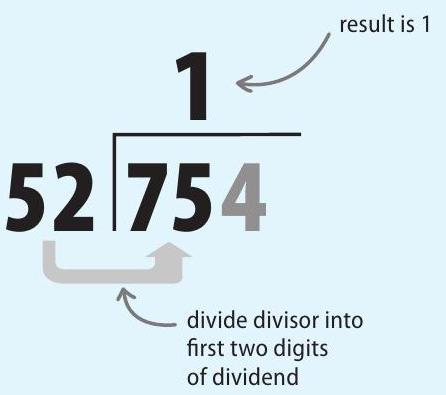
\includegraphics[max width=\textwidth, center]{2025_07_08_04014fa2c17a4b6cdcc6g-027}

Begin by dividing the divisor into the first two digits of the dividend. 52 fits into 75 once, so put a 1 above the dividing line, aligning it with the last digit of the number being divided.\\
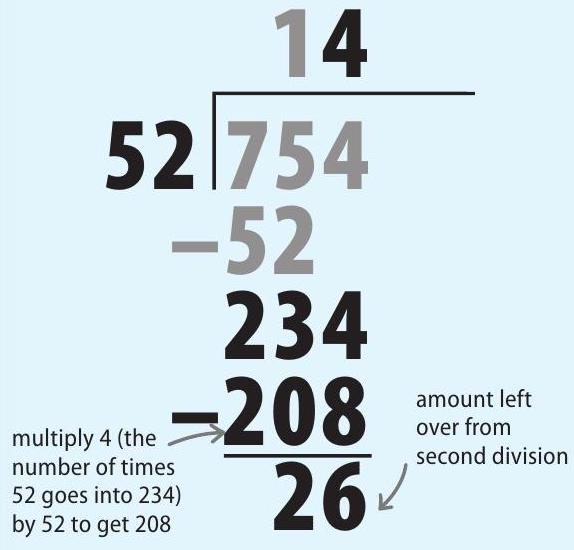
\includegraphics[max width=\textwidth, center]{2025_07_08_04014fa2c17a4b6cdcc6g-027(1)}

Work out the second remainder.\\
The divisor, 52, does not divide into 234 exactly. To find the remainder, multiply 4 by 52 to make 208.\\
Subtract 208 from 234, leaving 26.\\
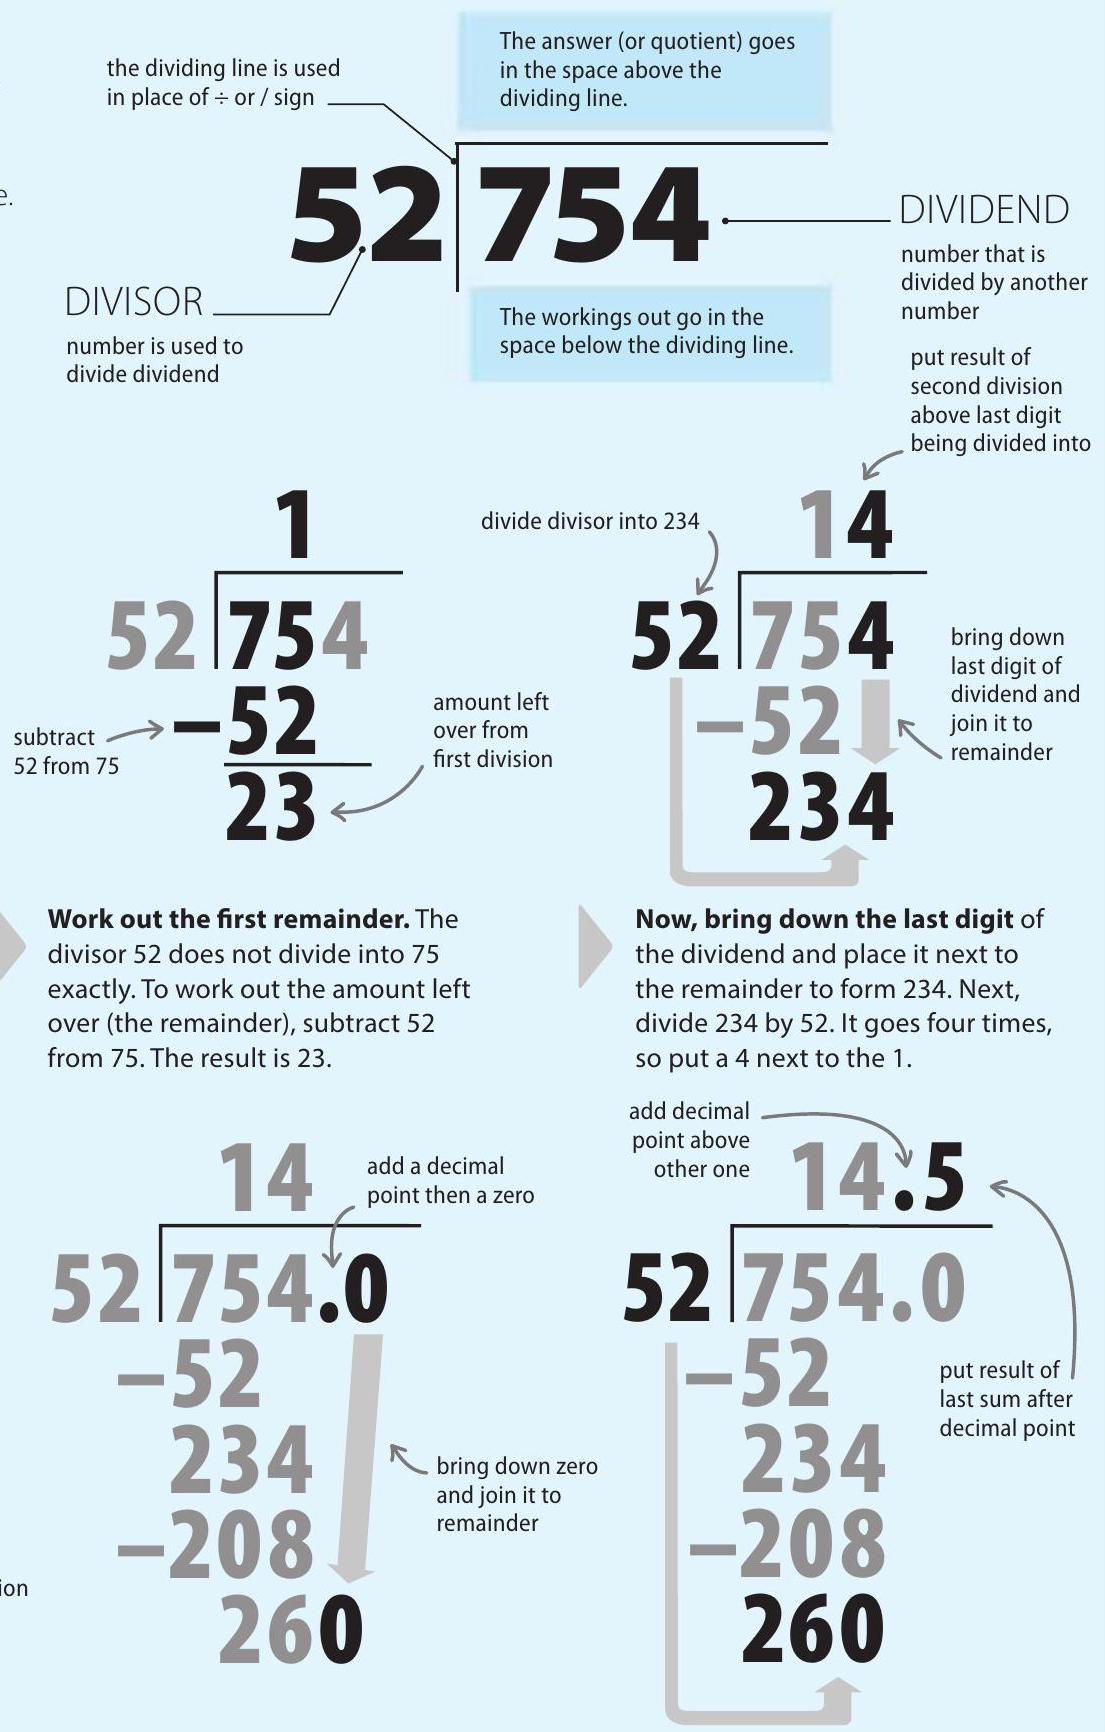
\includegraphics[max width=\textwidth, center]{2025_07_08_04014fa2c17a4b6cdcc6g-027(2)}

There are no more whole numbers to bring down, so add a decimal point after the dividend and a zero after it. Bring down the zero and join it to the remainder 26 to form 260.

Put a decimal point after the 14.\\
Next, divide 260 by 52, which goes five times exactly. Put a 5 above the dividing line, aligned with the new zero in the dividend.

\section*{11 Prime numbers}
ANY WHOLE NUMBER LARGER THAN 1 THAT CANNOT BE DIVIDED BY ANY OTHER NUMBER EXCEPT FOR ITSELF AND 1.

\section*{Introducing prime numbers}
Over 2,000 years ago, the Ancient Greek mathematician Euclid noted that some numbers are only divisible by 1 or the number itself. These numbers are known as prime numbers. A number that is not a prime is called a composite - it can be arrived at, or composed, by multiplying together smaller prime numbers, which are known as its prime factors.\\
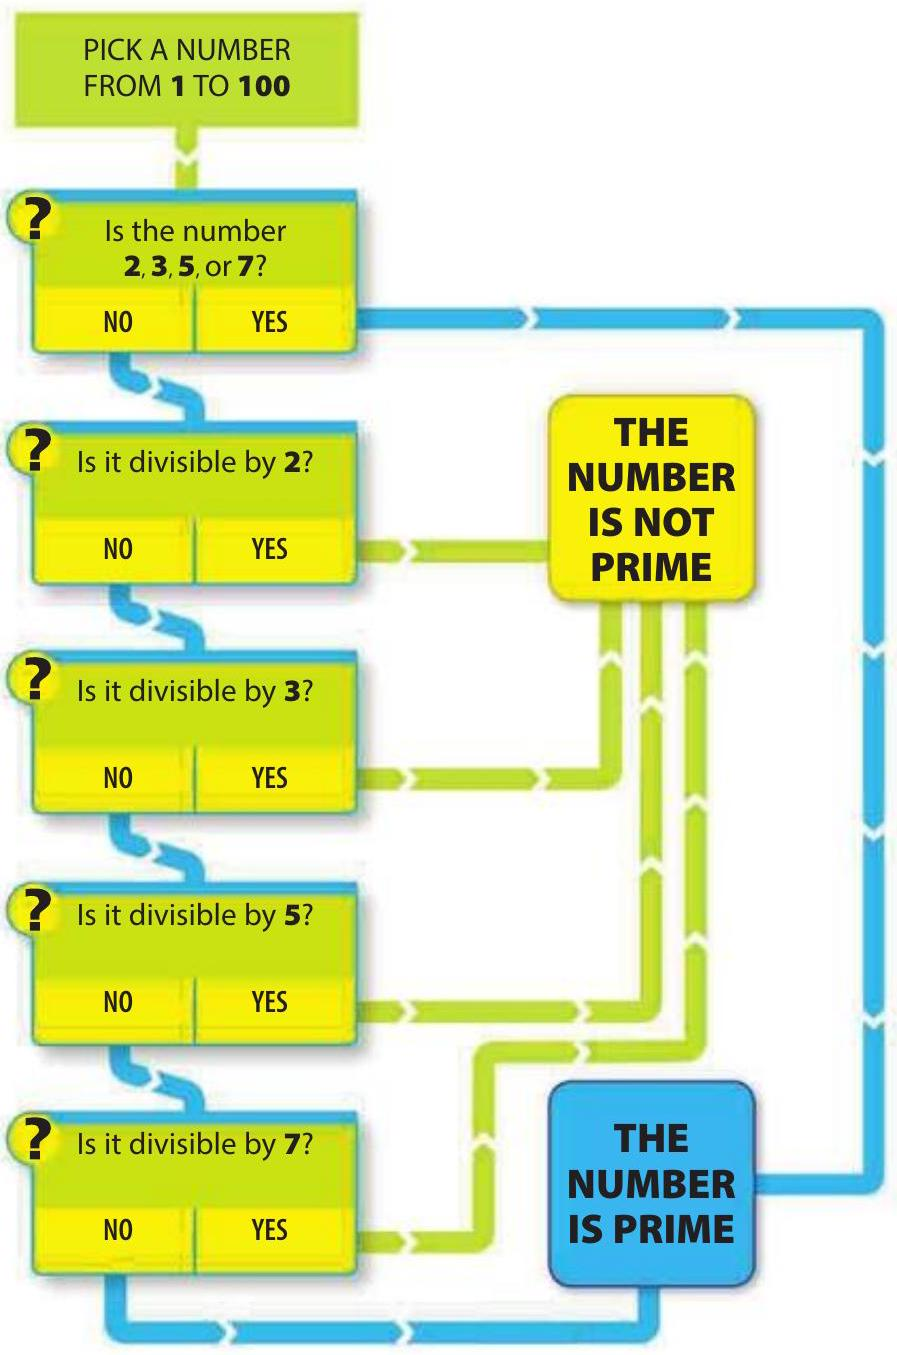
\includegraphics[max width=\textwidth, center]{2025_07_08_04014fa2c17a4b6cdcc6g-028(13)}\\
$\triangle$ Is a number prime?\\
This flowchart can be used to determine whether a number between 1 and 100 is prime by checking if it is divisible by any of the primes $2,3,5$, and 7 .

\section*{- First 100 numbers}
This table shows the prime numbers among the first 100 whole numbers.

\begin{center}
\begin{tabular}{|l|l|l|l|l|}
\hline
\multicolumn{5}{|c|}{2 is the only even prime number. Every other even number is not prime as they are all divisible by 2} \\
\hline

\includegraphics[max width=\textwidth]{2025_07_08_04014fa2c17a4b6cdcc6g-028(8)}
 & 
\includegraphics[max width=\textwidth]{2025_07_08_04014fa2c17a4b6cdcc6g-028(4)}
 & 
\includegraphics[max width=\textwidth]{2025_07_08_04014fa2c17a4b6cdcc6g-028(9)}
 & 2 & 
\includegraphics[max width=\textwidth]{2025_07_08_04014fa2c17a4b6cdcc6g-028(5)}
 \\
\hline
4 & 23 & 
\includegraphics[max width=\textwidth]{2025_07_08_04014fa2c17a4b6cdcc6g-028(6)}
 & 27 & 35 \\
\hline
37 & 2 & 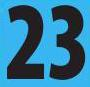
\includegraphics[max width=\textwidth]{2025_07_08_04014fa2c17a4b6cdcc6g-028}
 & \begin{tabular}{l}
24 \\
23 \\
\end{tabular} & 5 \\
\hline
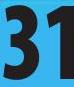
\includegraphics[max width=\textwidth]{2025_07_08_04014fa2c17a4b6cdcc6g-028(3)}
 & 2 & 3 & 2 & 57 \\
\hline
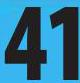
\includegraphics[max width=\textwidth]{2025_07_08_04014fa2c17a4b6cdcc6g-028(11)}
 & 2 & 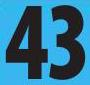
\includegraphics[max width=\textwidth]{2025_07_08_04014fa2c17a4b6cdcc6g-028(2)}
 & \begin{tabular}{l}
41 \\
2 \\
\end{tabular} & \begin{tabular}{l}
3 \\
5 \\
\end{tabular} \\
\hline
3 & 2 & 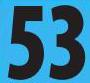
\includegraphics[max width=\textwidth]{2025_07_08_04014fa2c17a4b6cdcc6g-028(7)}
 & \begin{tabular}{l}
54 \\
23 \\
\end{tabular} & 5 \\
\hline
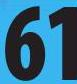
\includegraphics[max width=\textwidth]{2025_07_08_04014fa2c17a4b6cdcc6g-028(12)}
 & 2 & 37 & 2 & 5 \\
\hline
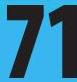
\includegraphics[max width=\textwidth]{2025_07_08_04014fa2c17a4b6cdcc6g-028(10)}
 & 23 & 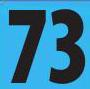
\includegraphics[max width=\textwidth]{2025_07_08_04014fa2c17a4b6cdcc6g-028(1)}
 & 2 & 35 \\
\hline
3 & 2 & 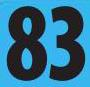
\includegraphics[max width=\textwidth]{2025_07_08_04014fa2c17a4b6cdcc6g-028(14)}
 & \begin{tabular}{l}
2 \\
3 \\
7 \\
\end{tabular} & 5 \\
\hline
7 & 2 & 3 & 2 & 5 \\
\hline
\end{tabular}
\end{center}

\begin{center}
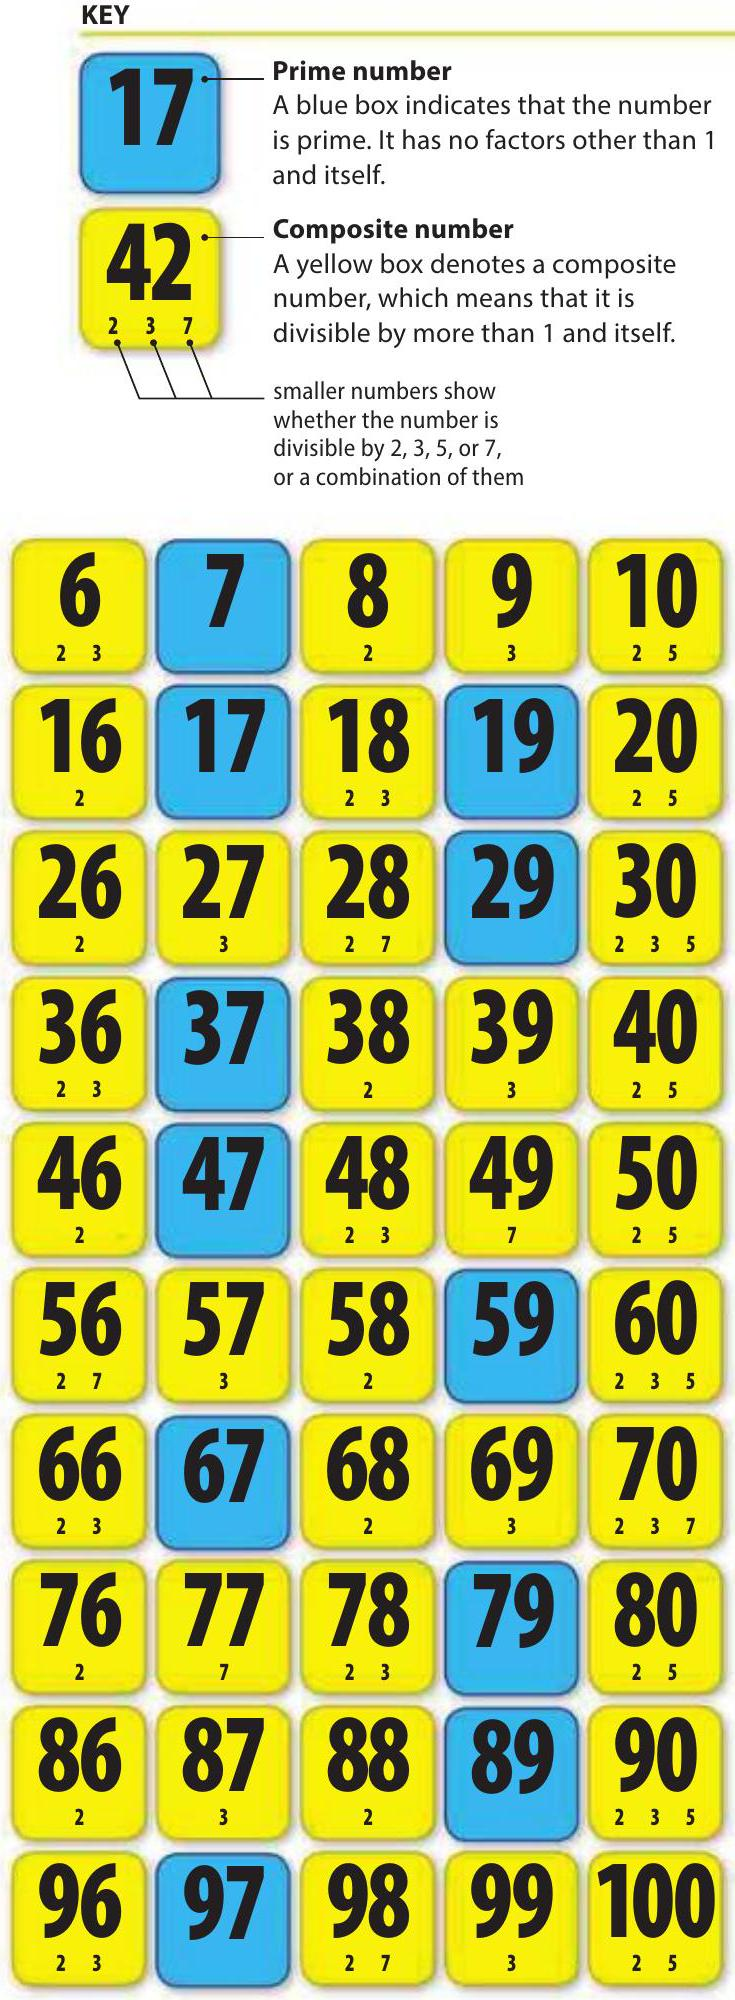
\includegraphics[max width=\textwidth]{2025_07_08_04014fa2c17a4b6cdcc6g-029(3)}
\end{center}

\section*{Prime factors}
Every number is either a prime or the result of multiplying together prime numbers. Prime factorization is the process of breaking down a composite number into the prime numbers that it is made up of. These are known as its prime factors.\\
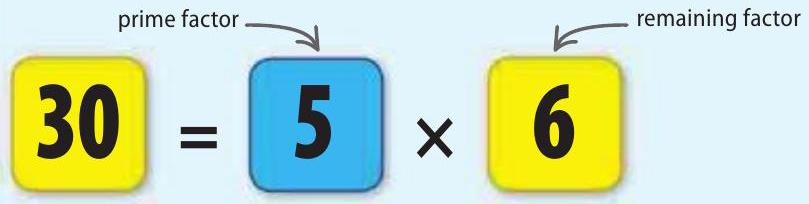
\includegraphics[max width=\textwidth, center]{2025_07_08_04014fa2c17a4b6cdcc6g-029(2)}

To find the prime factors of 30 , find the largest prime number that divides into 30 , which is 5 . The remaining factor is $6(5 \times 6=30)$, which needs to be broken down into prime numbers.\\
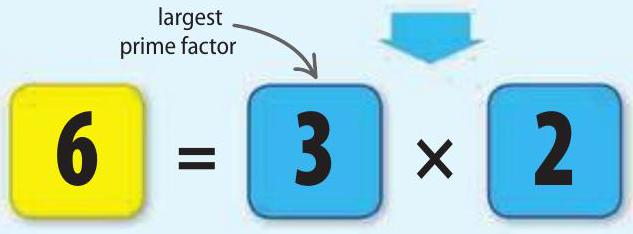
\includegraphics[max width=\textwidth, center]{2025_07_08_04014fa2c17a4b6cdcc6g-029}

Next, take the remaining factor and find the largest prime number that divides into it, and any smaller prime numbers. In this case, the prime numbers that divide into 6 are 3 and 2.\\
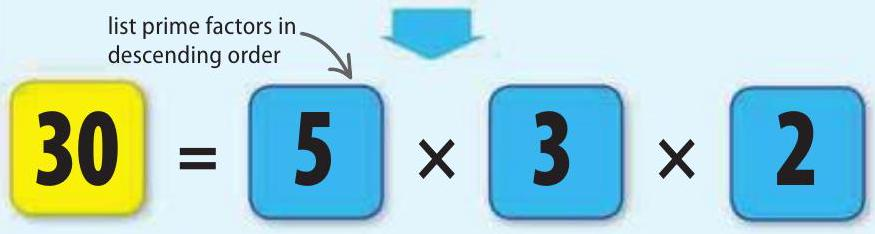
\includegraphics[max width=\textwidth, center]{2025_07_08_04014fa2c17a4b6cdcc6g-029(1)}

It is now possible to see that 30 is the product of multiplying together the prime numbers 5,3 , and 2 . Therefore, the prime factors of 30 are 5, 3, and, 2.

\section*{REAL WORLD}
\section*{Encryption}
Many transactions in banks and shops rely on the Internet and other communications systems. To protect the information, it is coded using a number that is the product of just two huge primes. The security relies on the fact that no "eavesdropper" can factorize the number because its factors are so large.

\section*{$\triangleright$ Data protection}
To provide constant security, mathematicians relentlessly hunt for ever bigger primes.\\
fldjhg83asldkfdslkfjour523ijwli eorit84wodfpflciry38s0x8b6lkj qpeoith73kdicuvyebdkciurmol wpeodikrucnyr83iowp7uhjwm kdieolekdoripasswordqe8ki mdkdoritut6483kednffkeoskeo kdieujr83iowplwqpwo98irkldil ieow98mqloapkijuhrnmeuidy6 woqp90jqiuke4Imicunejwkiuyj

\section*{Basic units}
\section*{Units of measurement}
UNITS OF MEASUREMENT ARE STANDARD SIZES USED TO MEASURE TIME，MASS，AND LENGTH．\\
A unit is any agreed or standardized measurement of size．This allows quantities to be accurately measured．There are three basic units：time， weight（including mass），and length．\\
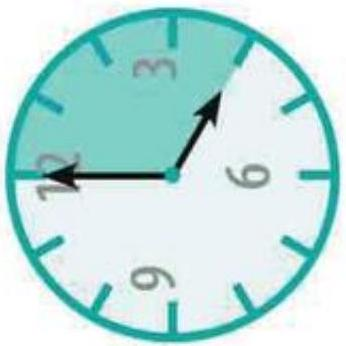
\includegraphics[max width=\textwidth, center]{2025_07_08_04014fa2c17a4b6cdcc6g-030(2)}\\
$\triangle$ Time\\
Time is measured in milliseconds， seconds，minutes，hours，days，weeks， months，and years．Different countries and cultures may have calendars which start a new year at a different time．

\section*{Compound measures}
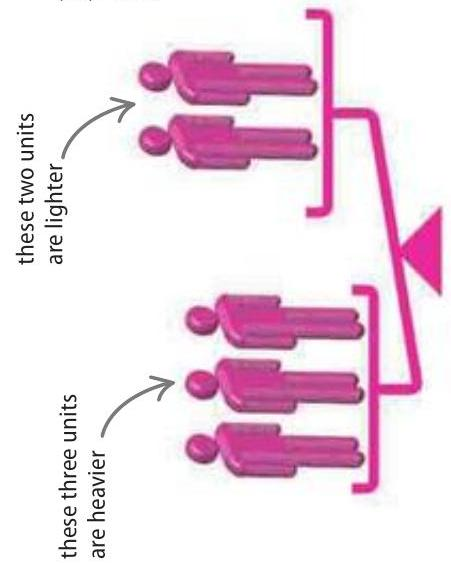
\includegraphics[max width=\textwidth, center]{2025_07_08_04014fa2c17a4b6cdcc6g-030(4)}\\
$\triangle$ Weight and mass\\
Weight is how heavy something is in relation to the force of gravity acting upon it．Mass is the amount of matter that makes up the object． Both are measured in the same units，such as grams and kilograms，or ounces and pounds．\\
A compound unit is made up of more than one of the basic units，including using the same unit repeatedly．Examples include area，volume，speed，and density．\\
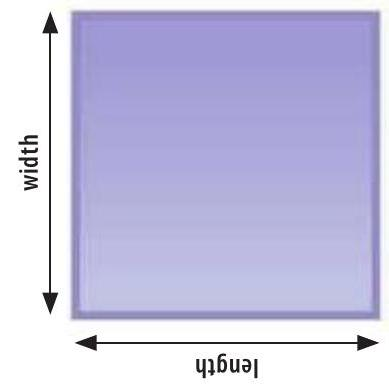
\includegraphics[max width=\textwidth, center]{2025_07_08_04014fa2c17a4b6cdcc6g-030(1)}

\section*{$\triangleleft$ Area}
Area is measured in squared units．The area of a square is the product of its length and width；if they were both measured in metres（ m ），its area would be $\mathrm{m} \times \mathrm{m}$ ，which is written as $\mathrm{m}^{2}$ ．

\begin{displayquote}
area $=$ length $\times$ width\\
area is made up of two of the same units，as width is also a length\\
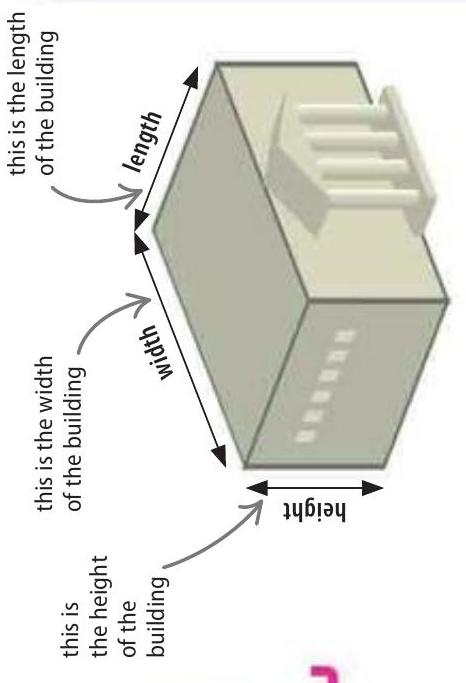
\includegraphics[max width=\textwidth, center]{2025_07_08_04014fa2c17a4b6cdcc6g-030(5)}\\
$\triangle$ Length\\
Length is how long something is．It is measured in centimetres，metres， and kilometres in the metric system， or in inches，feet，yards，and miles in the imperial system（see pp．242－245）．\\
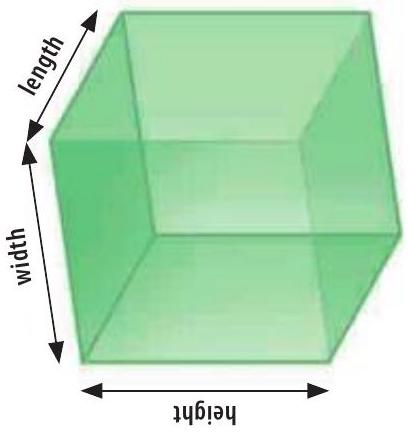
\includegraphics[max width=\textwidth, center]{2025_07_08_04014fa2c17a4b6cdcc6g-030(3)}
\end{displayquote}

\section*{Distance}
The distance is the amount of space between two points．It expresses length，but is also used to describe a journey， which is not always the most direct route between two points． plane flies set distance between two cities\\
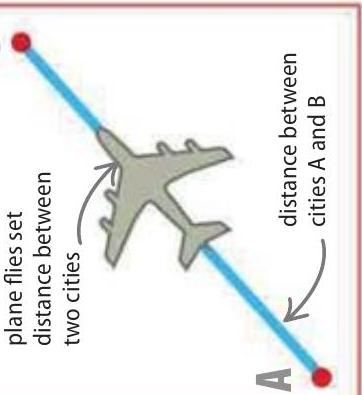
\includegraphics[max width=\textwidth, center]{2025_07_08_04014fa2c17a4b6cdcc6g-030}

\section*{$\triangleleft$ Volume}
Volume is measured in cubed units．The volume of a cuboid is the product of its height，width， and length；if they were all measured in metres （m），its area would be $m \times m \times m$ ，or $m^{3}$ ．

$$
\text { volume }=\text { length } \times \text { width } \times \text { height }
$$

volume is a compound of three of the same units，as width and height are technically lengths

\section*{Speed}
Speed measures the distance (length) travelled in a given time. This means that the formula for measuring speed is length $\div$ time. If this is measured in kilometres and hours, the unit for speed will be km/h.

$$
\text { Speed }=\frac{\text { distance }}{\text { time }}
$$

$\triangleright$ Speed formula triangle The relationships between speed, distance, and time can be shown in a triangle. The position of each unit in the triangle indicates how to use the other two measurements to calculate that unit.

\section*{Density}
\begin{center}
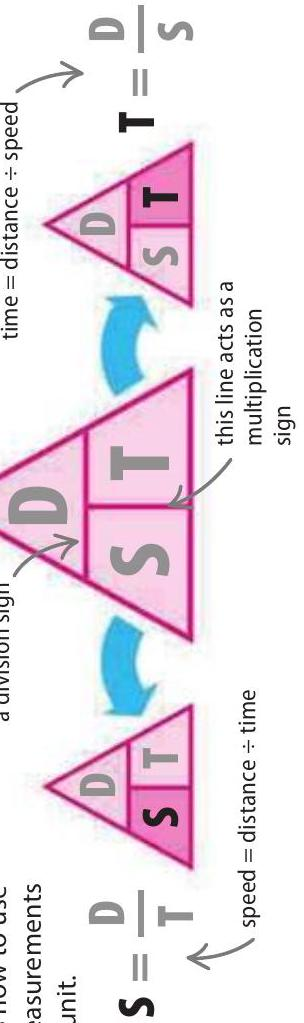
\includegraphics[max width=\textwidth]{2025_07_08_04014fa2c17a4b6cdcc6g-031(3)}
\end{center}

Density measures how much matter is packed into a given volume of a substance. It involves two units - mass and volume. The formula for measuring density is mass $\div$ volume. If this is measured in grams and centimetres, the unit for density will be $\mathrm{g} / \mathrm{cm}^{3}$.\\
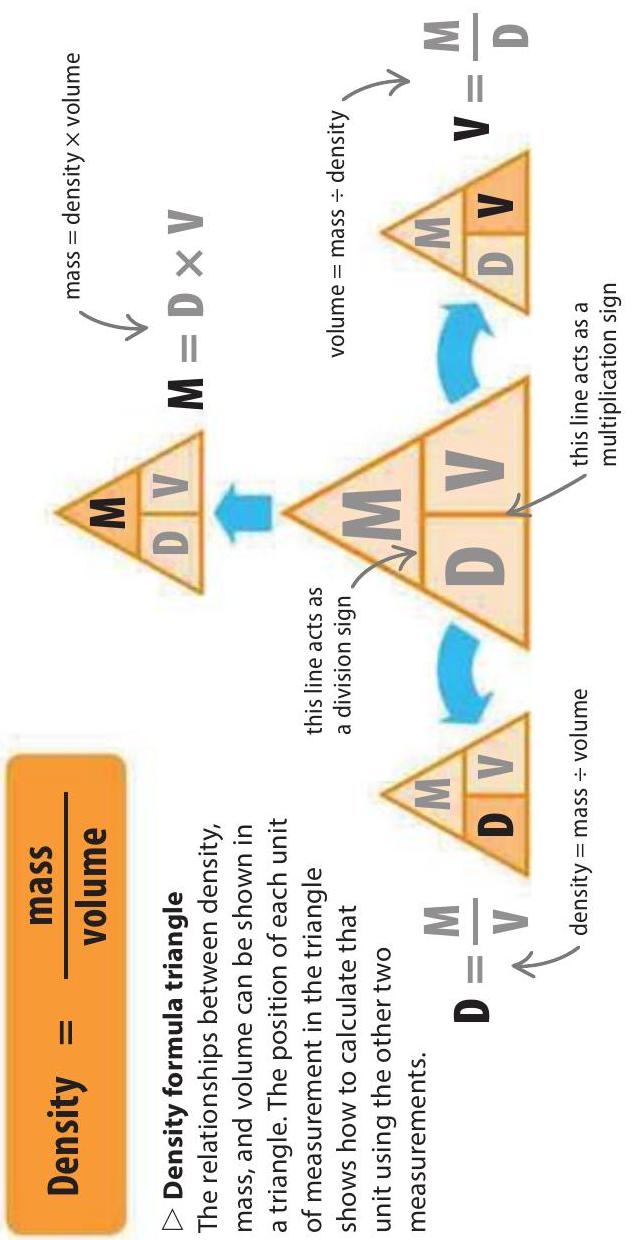
\includegraphics[max width=\textwidth, center]{2025_07_08_04014fa2c17a4b6cdcc6g-031(2)}

\section*{- Finding speed}
A van travels 20 km in 20 minutes. From this information its speed in $\mathrm{km} / \mathrm{h}$ can be found.\\
divide 20 by 60 to find its\\
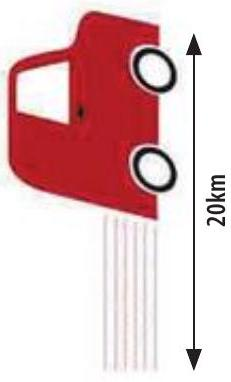
\includegraphics[max width=\textwidth, center]{2025_07_08_04014fa2c17a4b6cdcc6g-031(1)}

\section*{value in hours \\
 20 minutes $\Rightarrow \frac{20}{60}=\frac{1}{3}$ hour}
First, convert the minutes into hours. To convert minutes into hours, divide them by 60 , then cancel the fraction - divide the top and bottom numbers by 20 . This gives an answer of $1 / 3$ hour.

Then, substitute the values for distance and time into the formula for speed. Divide the distance ( 20 km ) by the time ( $1 / 3$ hour) to find the speed, in this case $60 \mathrm{~km} / \mathrm{h}$.

\section*{$\Delta$ Finding volume}
density of lead is\\
constant, regardless

Lead has a density of $0.0113 \mathrm{~kg} /$ $\mathrm{cm}^{3}$. With this measurement, the volume of a lead weight that has a mass of 0.5 kg can be found.

\section*{$\Delta$ Using the formula}
 of mass\begin{center}
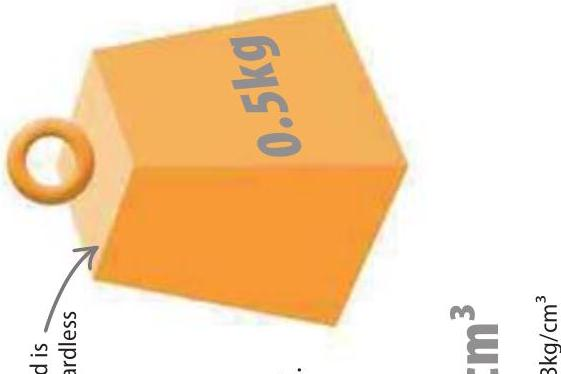
\includegraphics[max width=\textwidth]{2025_07_08_04014fa2c17a4b6cdcc6g-031}
\end{center}

Substitute the values for mass and density into the formula for volume. Divide the mass ( 0.5 kg ) by the density ( $0.0113 \mathrm{~kg} / \mathrm{cm}^{3}$ ) to find the volume, in this case $44.25 \mathrm{~cm}^{3}$.

\section*{Telling the time}
TIME IS MEASURED IN THE SAME WAY AROUND THE WORLD. THE MAIN UNITS ARE SECONDS, MINUTES, AND HOURS.\\
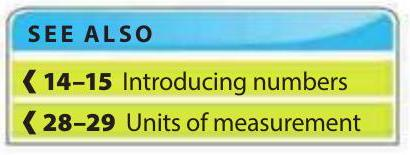
\includegraphics[max width=\textwidth, center]{2025_07_08_04014fa2c17a4b6cdcc6g-032}

\section*{Bigger units of time}
This is a list of the most commonly used bigger units of time. Other units include the Olympiad, which is a period of 4 years and starts on January 1st of a year in which the summer Olympics take place.

\section*{7 days is 1 week}
Fortnight is short for 14 nights and is the same as $\mathbf{2}$ weeks

\begin{displayquote}
Between 28 and 31 days is $\mathbf{1}$ month
\end{displayquote}

\section*{365 days is $\mathbf{1}$ year (366 in a leap year) \\
 10 years is a decade \\
 100 years is a century}
\section*{1000 years is a millennium}
\section*{Reading the time}
The time can be told by looking carefully at where the hands point on a clock or watch. The hour hand is shorter and moves around slowly. The minute hand is longer than the hour hand and points at minutes "past" the hour or "to" the next one. Most clock faces show the minutes in groups of five and the in-between minutes are shown by a short line or mark. The second hand is usually long and thin, and sweeps quickly around the face every minute, marking 60 seconds.\\
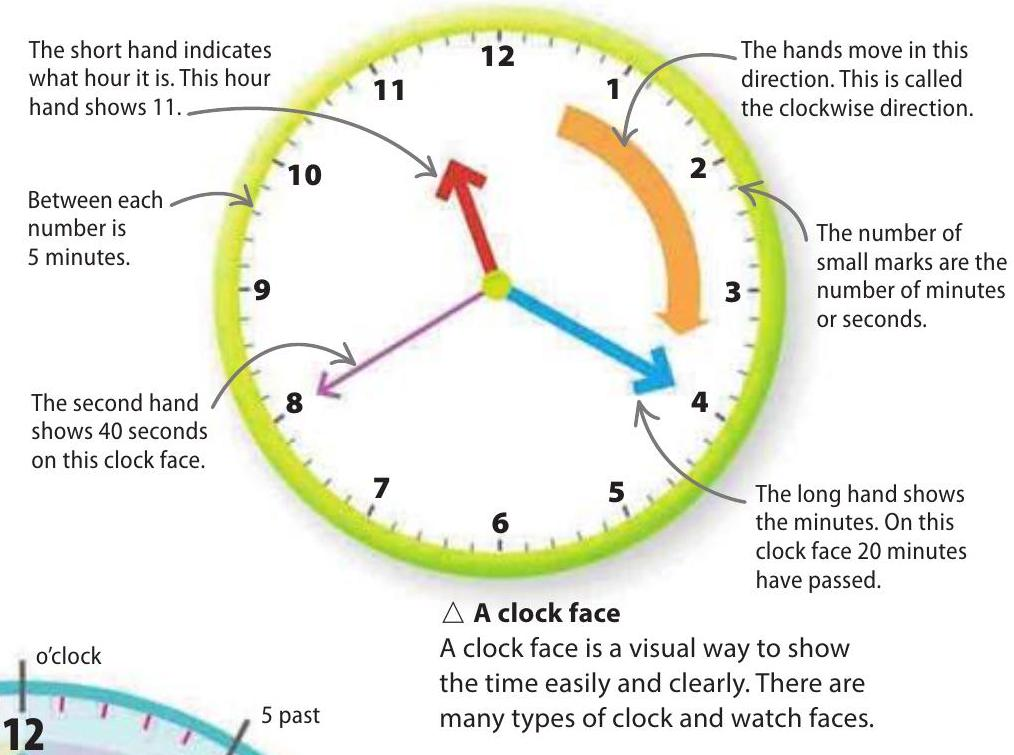
\includegraphics[max width=\textwidth, center]{2025_07_08_04014fa2c17a4b6cdcc6g-033(1)}\\
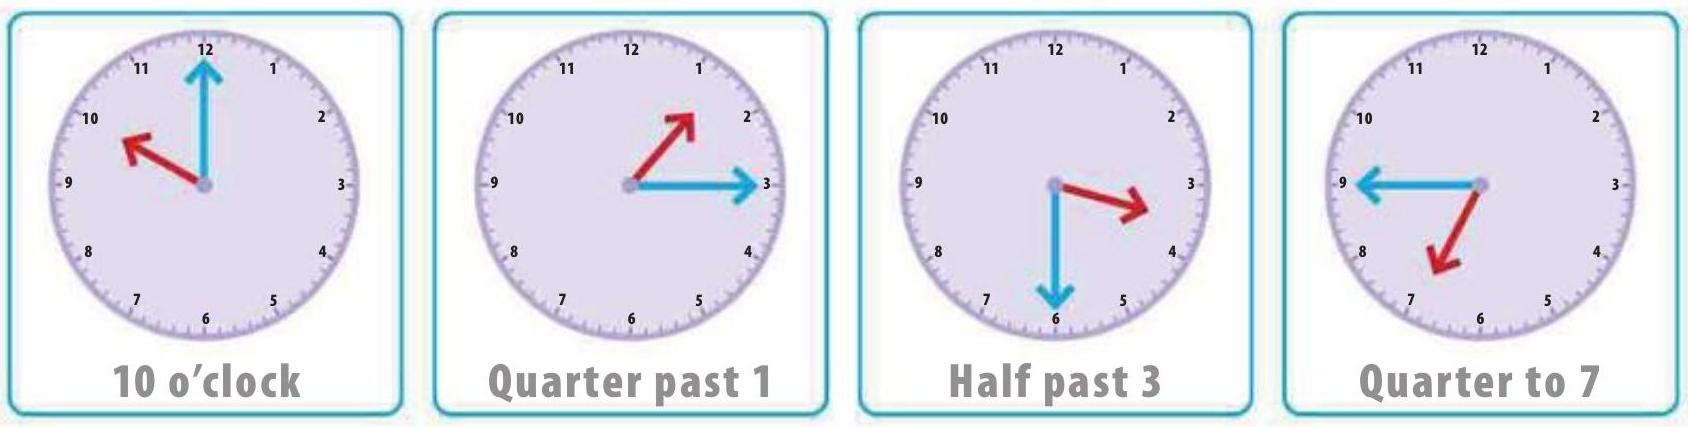
\includegraphics[max width=\textwidth, center]{2025_07_08_04014fa2c17a4b6cdcc6g-033}

\section*{Analogue time}
Most clocks and watches only go up to 12 hours, but there are 24 hours in one day. To show the difference between morning and night, we use AM or PM. The middle of the day ( 12 o'clock) is called midday or noon.\\
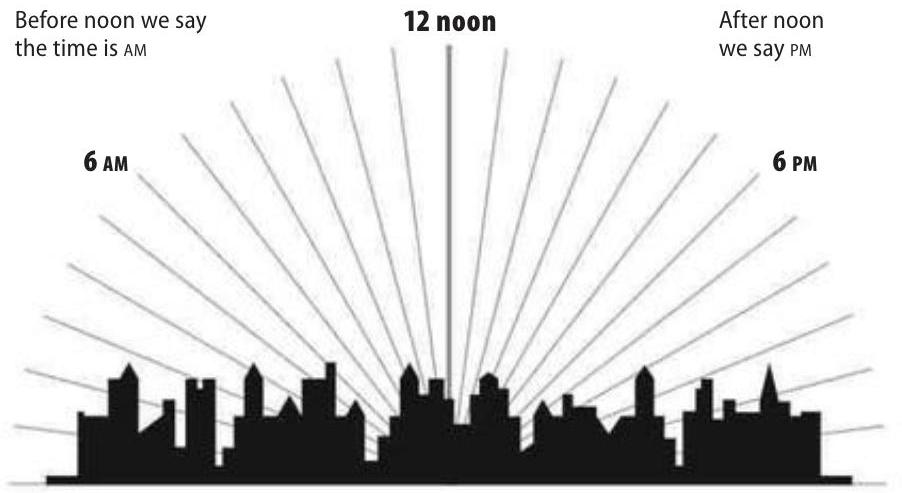
\includegraphics[max width=\textwidth, center]{2025_07_08_04014fa2c17a4b6cdcc6g-034(3)}\\
$\triangle \mathbf{A M}$ or PM\\
The initials AM and PM stand for the Latin words ante meridiem (meaning "before noon") and post meridiem (meaning "after noon"). The first 12 hours of the day are called AM and the second 12 hours of the day are called PM.

\section*{Digital time}
Traditional clock faces show time in an analogue format but digital formats are also common, especially on electrical devices such as computers, televisions, and mobile phones. Some digital displays show time in the 24 -hour system, others use the analogue system and also show AM or PM.\\
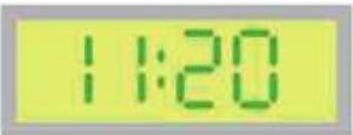
\includegraphics[max width=\textwidth, center]{2025_07_08_04014fa2c17a4b6cdcc6g-034(4)}

\section*{$\triangle$ Hours and minutes}
On a digital clock, the hours are shown first followed by a colon and the minutes. Some displays may also show seconds.\\
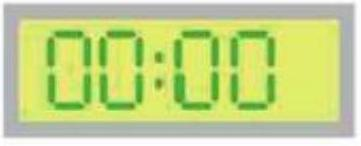
\includegraphics[max width=\textwidth, center]{2025_07_08_04014fa2c17a4b6cdcc6g-034(2)}

\section*{$\triangle$ Midnight}
When it is midnight, the clock resets to 00:00. Midnight is an abbreviated form of "middle of the night".\\
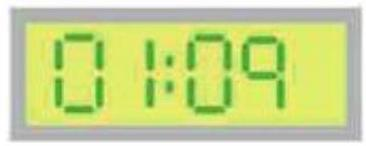
\includegraphics[max width=\textwidth, center]{2025_07_08_04014fa2c17a4b6cdcc6g-034}\\
$\Delta$ 24-hour digital display\\
If the hours or minutes are single digit numbers, a zero (called a leading zero) is placed to the left of the digit.\\
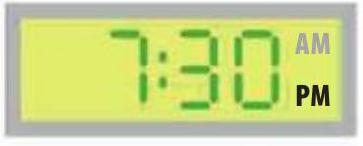
\includegraphics[max width=\textwidth, center]{2025_07_08_04014fa2c17a4b6cdcc6g-034(1)}\\
$\Delta$ 12-hour digital display This type of display will have AM and PM with the relevant part of the day highlighted.

\section*{24-hour clock}
The 24-hour system was devised to stop confusion between morning and afternoon times, and runs continuously from midnight to midnight. It is often used in computers, by the military, and on timetables. To convert from the 12-hour system to the 24-hour system, you add 12 to the hour for times after noon. For example, 11 PM becomes 23:00 (11 + 12) and 8:45 PM becomes 20:45 (8:45 + 12).

\begin{center}
\begin{tabular}{|l|l|}
\hline
12-hour clock & 24-hour clock \\
\hline
12:00 midnight & 00:00 \\
\hline
1:00 am & 01:00 \\
\hline
2:00 am & 02:00 \\
\hline
3:00 am & 03:00 \\
\hline
4:00 am & 04:00 \\
\hline
5:00 am & 05:00 \\
\hline
6:00 am & 06:00 \\
\hline
7:00 am & 07:00 \\
\hline
8:00 am & 08:00 \\
\hline
9:00 am & 09:00 \\
\hline
10:00 am & 10:00 \\
\hline
11:00 am & 11:00 \\
\hline
12:00 noon & 12:00 \\
\hline
1:00 PM & 13:00 \\
\hline
2:00 PM & 14:00 \\
\hline
3:00 PM & 15:00 \\
\hline
4:00 PM & 16:00 \\
\hline
5:00 PM & 17:00 \\
\hline
6:00 PM & 18:00 \\
\hline
7:00 PM & 19:00 \\
\hline
8:00 PM & 20:00 \\
\hline
9:00 PM & 21:00 \\
\hline
10:00 PM & 22:00 \\
\hline
11:00 PM & 23:00 \\
\hline
\end{tabular}
\end{center}

\section*{xvii Roman numerals}
\section*{DEVELOPED BY THE ANCIENT ROMANS, THIS SYSTEM USES LETTERS FROM THE LATIN ALPHABET TO REPRESENT NUMBERS.}
\section*{Understanding Roman numerals}
The Roman numeral system does not use zero. To make a number, seven letters are combined. These are the letters and their values:\\
I $\underset{1}{\text { V }} \underset{10}{\text { X }} \underset{50}{\text { L }} \underset{100}{\underset{500}{\text { C }}} \underset{1000}{\underset{\text { (D) }}{\text { M }}}$

\section*{Forming numbers}
Some key principles were observed by the ancient Romans to "create" numbers from the seven letters.

First principle When a smaller number appears after a larger number, the smaller number is added to the larger number to find the total value.

$$
X I=X+I=11 \quad X V I I=X+V+I+I=17
$$

Second principle When a smaller number appears before a larger number, the smaller number is subtracted from the larger number to find the total value.

$$
I X=X-I=9 \quad C M=M-C=900
$$

Third principle Each letter can be repeated up to three times.

$$
X X=X+X=20 \quad X X X=X+X+X=30
$$

\section*{Using Roman numerals}
Although Roman numerals are not widely used today, they still appear on some clock faces, with the names of monarchs and popes, and for important dates.\\
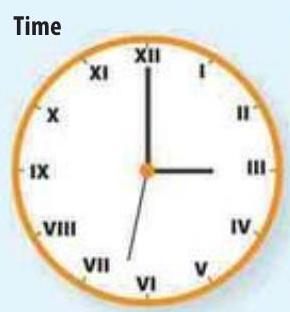
\includegraphics[max width=\textwidth, center]{2025_07_08_04014fa2c17a4b6cdcc6g-035}

Names

\section*{Henry VIII}
Henry the eighth

\section*{Dates}
MMXIV\\
2014

\section*{SEE ALSO}
《 14-15 Introducing\\
numbers

\begin{center}
\begin{tabular}{|l|l|}
\hline
Number & Roman numeral \\
\hline
1 & I \\
\hline
2 & II \\
\hline
3 & III \\
\hline
4 & IV \\
\hline
5 & v \\
\hline
6 & VI \\
\hline
7 & VII \\
\hline
8 & VIII \\
\hline
9 & IX \\
\hline
10 & X \\
\hline
11 & XI \\
\hline
12 & XII \\
\hline
13 & XIII \\
\hline
14 & XIV \\
\hline
15 & XV \\
\hline
16 & XVI \\
\hline
17 & XVII \\
\hline
18 & XVIII \\
\hline
19 & XIX \\
\hline
20 & XX \\
\hline
30 & XXX \\
\hline
40 & XL \\
\hline
50 & L \\
\hline
60 & LX \\
\hline
70 & LXX \\
\hline
80 & LXXX \\
\hline
90 & XC \\
\hline
100 & C \\
\hline
500 & D \\
\hline
1000 & M \\
\hline
\end{tabular}
\end{center}

\section*{+- Positive and negative numbers}
\section*{A POSITIVE NUMBER IS A NUMBER THAT IS MORE THAN ZERO (NOUGHT), WHILE A NEGATIVE NUMBER IS LESS THAN ZERO.}
A positive number is shown by a plus sign (+), or has no sign in front of it. If a number is negative, it has a minus sign ( - ) in front of it.

\begin{verbatim}
SEE ALSO
< 14-15 Introducing numbers
< 16-17 Addition and
subtraction
\end{verbatim}

\section*{Why use positives and negatives?}
Positive numbers are used when an amount is counted up from zero, and negative numbers when it is counted down from zero. For example, if a bank account has money in it, it is a positive amount of money, but if the account is overdrawn, the amount of money in the account is negative.

\section*{Adding and subtracting positives and negatives}
Use a number line to add and subtract positive and negative numbers. Find the first number on the line and then move the number of steps shown by the second number. Move right for addition and left for subtraction.\\
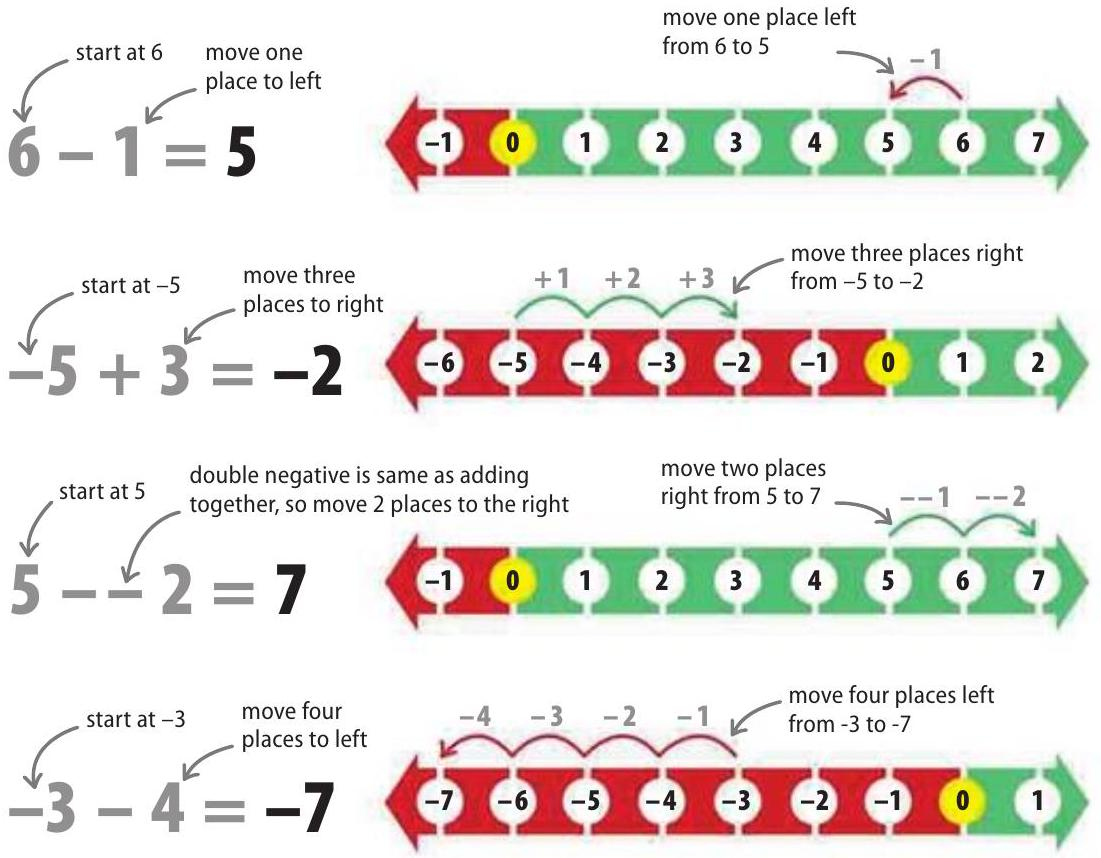
\includegraphics[max width=\textwidth, center]{2025_07_08_04014fa2c17a4b6cdcc6g-036}

\section*{LOOKING CLOSER}
\section*{Double negatives}
If a negative or minus number is subtracted from a positive number, it creates a double negative. As the first negative is cancelled out by the second negative, the result is always a positive; for example 5 minus -2 is the same as adding 2 to 5.\\
ఉ = =\\
$\Delta$ Like signs equal a positive\\
If any two like signs appear together, the result is always positive. The result is negative with two unlike signs together.

\section*{$\nabla$ Number line}
A number line is a good way to get to grips with positive and negative numbers. Draw the positive numbers to the right of 0 , and the negative numbers to the left of 0 . Adding colour makes them easier to tell apart.

\section*{REAL WORLD}
\section*{Thermometer}
Negative numbers are necessary to record temperatures, as during the winter they can fall well below $0^{\circ} \mathrm{C}$, which is freezing point. The lowest temperature that has ever been recorded is $-89.2^{\circ} \mathrm{C}\left(-128.6^{\circ} \mathrm{F}\right)$, in Antarctica.\\
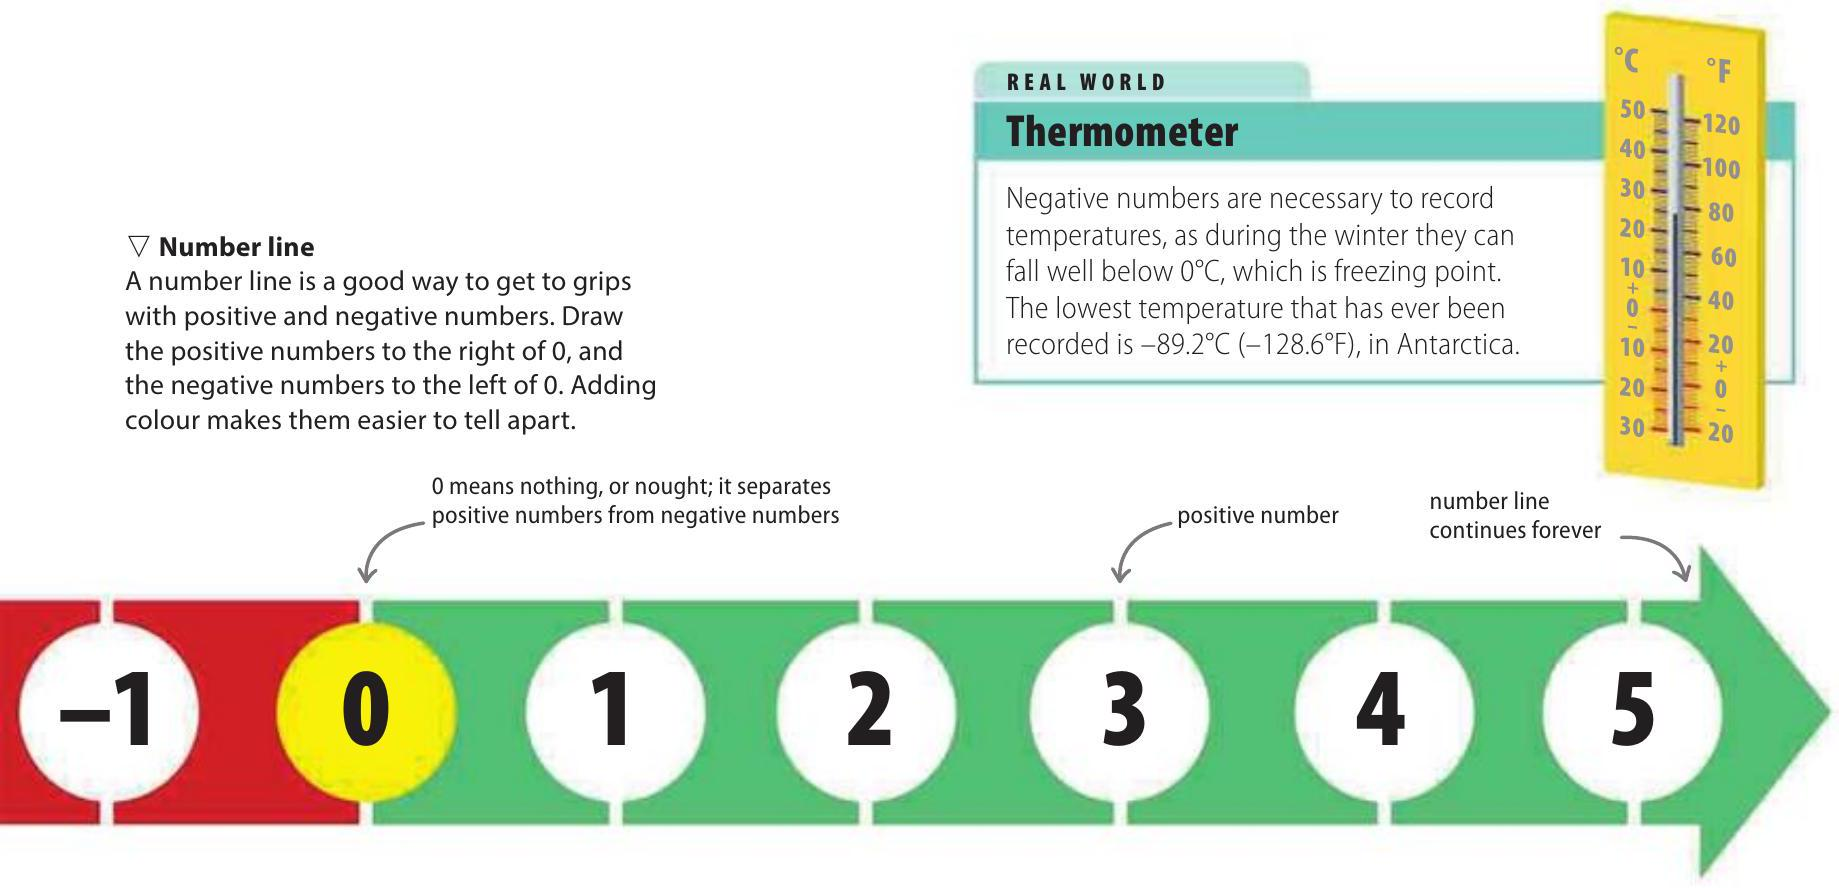
\includegraphics[max width=\textwidth, center]{2025_07_08_04014fa2c17a4b6cdcc6g-037(2)}

\section*{Multiplying and dividing}
To multiply or divide any two numbers, do the sum ignoring whether they are positive or negative, then work out if the answer is positive or negative using the diagram on the right.\\
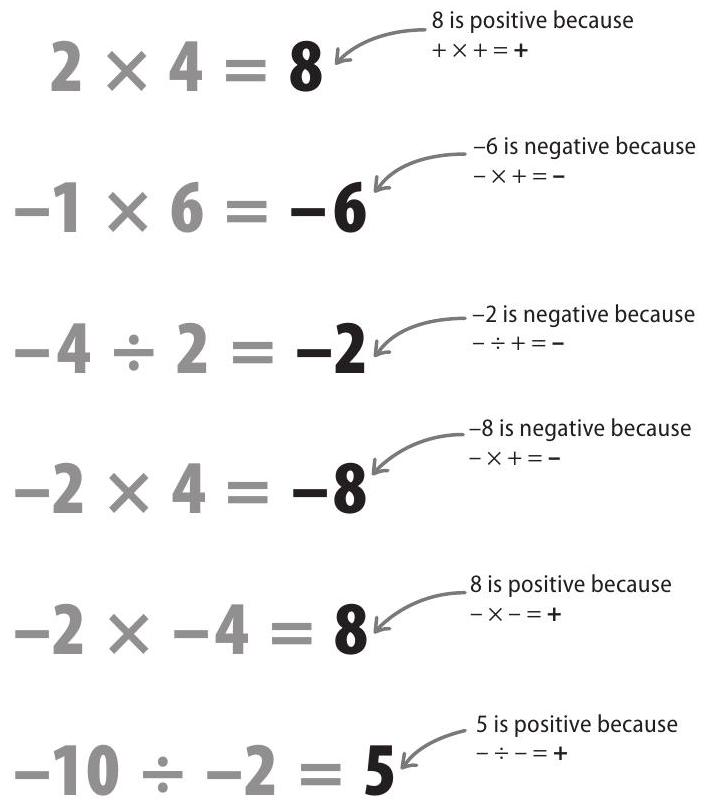
\includegraphics[max width=\textwidth, center]{2025_07_08_04014fa2c17a4b6cdcc6g-037(1)}\\
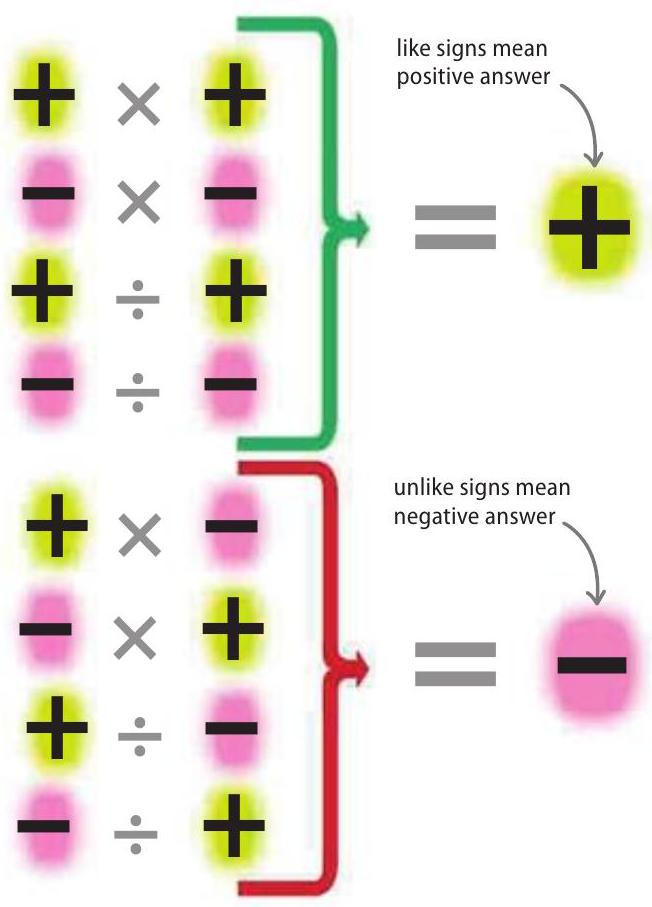
\includegraphics[max width=\textwidth, center]{2025_07_08_04014fa2c17a4b6cdcc6g-037}

\section*{Positive or negative answer}
The sign in the answer depends on whether the signs of the numbers are alike or not.

\section*{$\checkmark$Powers and roots }
\section*{A POWER IS THE NUMBER OF TIMES A NUMBER IS MULTIPLIED BY ITSELF. THE ROOT OF A NUMBER IS A NUMBER WHICH, MULTIPLIED BY ITSELF, EQUALS THE ORIGINAL NUMBER.}
\begin{center}
\begin{tabular}{|l|l|}
\hline
SEE ALSO &  \\
\hline
《18-21 & Multiplication \\
\hline
(22-25 & Division \\
\hline
Standard form & $\mathbf{4 2 - 4 3} \boldsymbol{>}$ \\
\hline
\begin{tabular}{l}
Using a \\
calculator \\
\end{tabular} & $\mathbf{7 2 - 7 3} \boldsymbol{>}$ \\
\hline
\end{tabular}
\end{center}

\section*{Introducing powers}
A power is the number of times a number is multiplied by itself. This is indicated as a smaller number positioned to the right above the number. Multiplying a number by itself once is described as "squaring" the number; multiplying a number by itself twice is described as\\
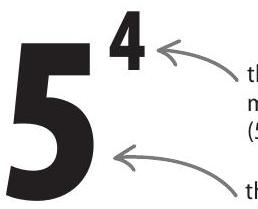
\includegraphics[max width=\textwidth]{2025_07_08_04014fa2c17a4b6cdcc6g-038} this is the power, which shows how many times to multiply the number ( $5^{4}$ means $5 \times 5 \times 5 \times 5$ )\\
this is the number that the power relates to "cubing" the number.\\
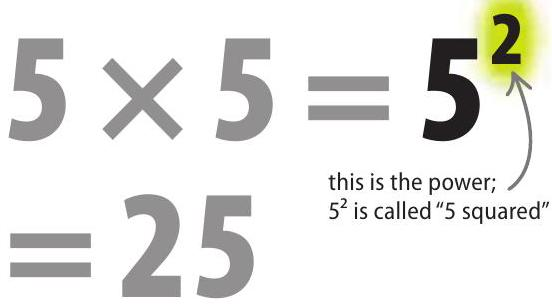
\includegraphics[max width=\textwidth, center]{2025_07_08_04014fa2c17a4b6cdcc6g-038(1)}

\section*{$\triangle$ The square of a number}
Multiplying a number by itself gives the square of the number. The power for a square number is ${ }^{2}$, for example $5^{2}$, which means there are 2 lots of 5 or $5 \times 5$.\\
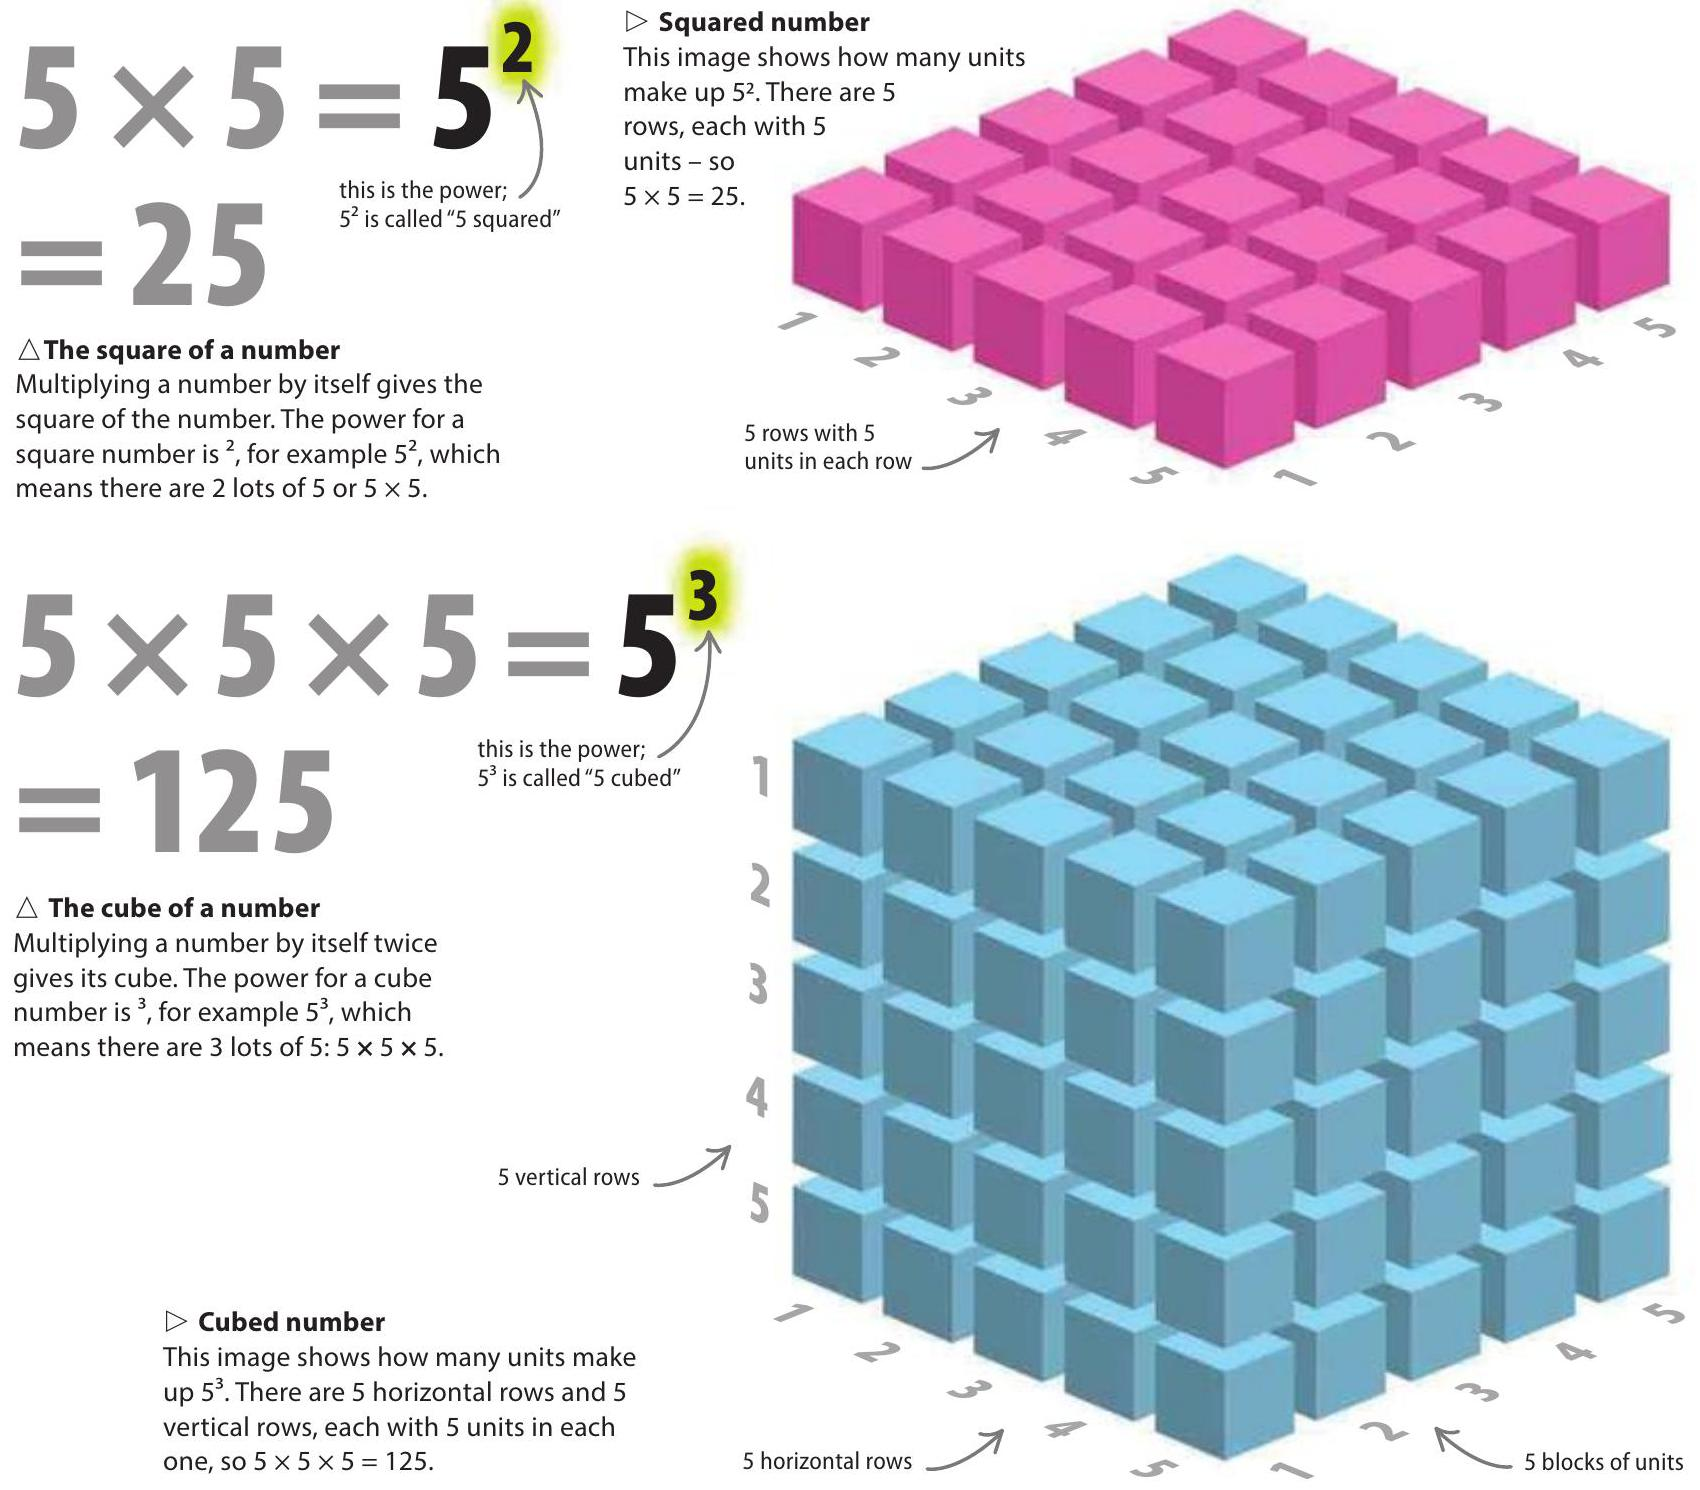
\includegraphics[max width=\textwidth, center]{2025_07_08_04014fa2c17a4b6cdcc6g-038(2)}

\section*{Square roots and cube roots}
A square root is a number which, multiplied by itself once, equals a given number. For example, one square root of 4 is 2 , as $2 \times 2=4$. Another square root is -2 , as $(-2) \times(-2)=4$. The square roots of numbers can be either positive or negative. A cube root is a number which, multiplied by itself twice, equals a given number. For example, the cube root of 27 is 3 , as $3 \times 3 \times 3=27$.

\section*{$\sqrt{25}=5$ because $5 \times 5=25^{2}$}
\section*{$\triangle$ The square root of a number}
The square root of a number is the number which, when squared (multiplied by itself), equals the number under the square root sign.

\section*{$\sqrt[3]{125}=\mathbf{5}_{\text {beause }} 5 \times 5 \times 5=125$}
\section*{The cube root of a number}
The cube root of a number is the number which, when cubed (multiplied by itself twice), equals the number under the cube root sign.

\begin{center}
\begin{tabular}{|l|l|l|}
\hline
\multicolumn{3}{|c|}{COMMON SQUARE ROOTS} \\
\hline
Square root & Answer & Why? \\
\hline
1 & 1 & Because $1 \times 1=1$ \\
\hline
4 & 2 & Because $2 \times 2=4$ \\
\hline
9 & 3 & Because $3 \times 3=9$ \\
\hline
16 & 4 & Because $4 \times 4=16$ \\
\hline
25 & 5 & Because $5 \times 5=25$ \\
\hline
36 & 6 & Because $6 \times 6=36$ \\
\hline
49 & 7 & Because $7 \times 7=49$ \\
\hline
64 & 8 & Because $8 \times 8=64$ \\
\hline
81 & 9 & Because $9 \times 9=81$ \\
\hline
100 & 10 & Because $10 \times 10=100$ \\
\hline
121 & 11 & Because $11 \times 11=121$ \\
\hline
144 & 12 & Because $12 \times 12=144$ \\
\hline
169 & 13 & Because $13 \times 13=169$ \\
\hline
\end{tabular}
\end{center}

\section*{LOOKING CLOSER}
\section*{Using a calculator}
Calculators can be used to find powers and square roots. Most calculators have buttons to square and cube numbers, buttons to find square roots and cube roots, and an exponent button, which allows them to raise numbers to any power.\\
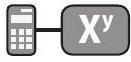
\includegraphics[max width=\textwidth, center]{2025_07_08_04014fa2c17a4b6cdcc6g-039}

\section*{$\triangle$ Exponent}
This button allows any number to be raised to any power.\\
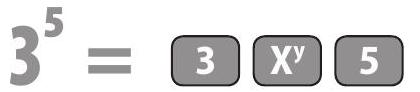
\includegraphics[max width=\textwidth, center]{2025_07_08_04014fa2c17a4b6cdcc6g-039(1)}

$$
\text { = } 243
$$

This button allows the square root of any number to be

$$
\begin{aligned}
25 & =\square \\
& =\mathbf{5}
\end{aligned}
$$ found.

\section*{$\checkmark$ Using exponents}
First enter the number to be raised to a power, then press the exponent button, then enter the power required.

\section*{$\triangleleft$ Using square roots}
On most calculators, find the square root of a number by pressing the square root button first and then entering the number.

\section*{Multiplying powers of the same number}
To multiply powers that have the same number simply add the powers. The power of the answer is the sum of the powers that are being multiplied.\\
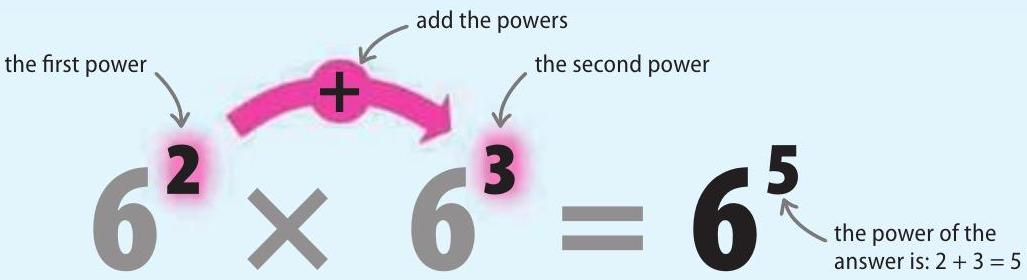
\includegraphics[max width=\textwidth, center]{2025_07_08_04014fa2c17a4b6cdcc6g-040(3)}\\
because

\section*{- Writing it out}
Writing out what each of these powers represents shows why powers are added together to multiply them.\\
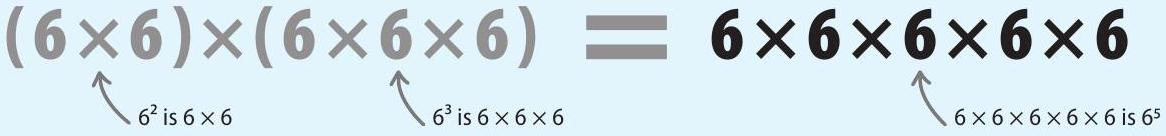
\includegraphics[max width=\textwidth, center]{2025_07_08_04014fa2c17a4b6cdcc6g-040(1)}

\section*{Dividing powers of the same number}
To divide powers of the same number, subtract the second power from the first. The power of the answer is the difference between the first and second powers.\\
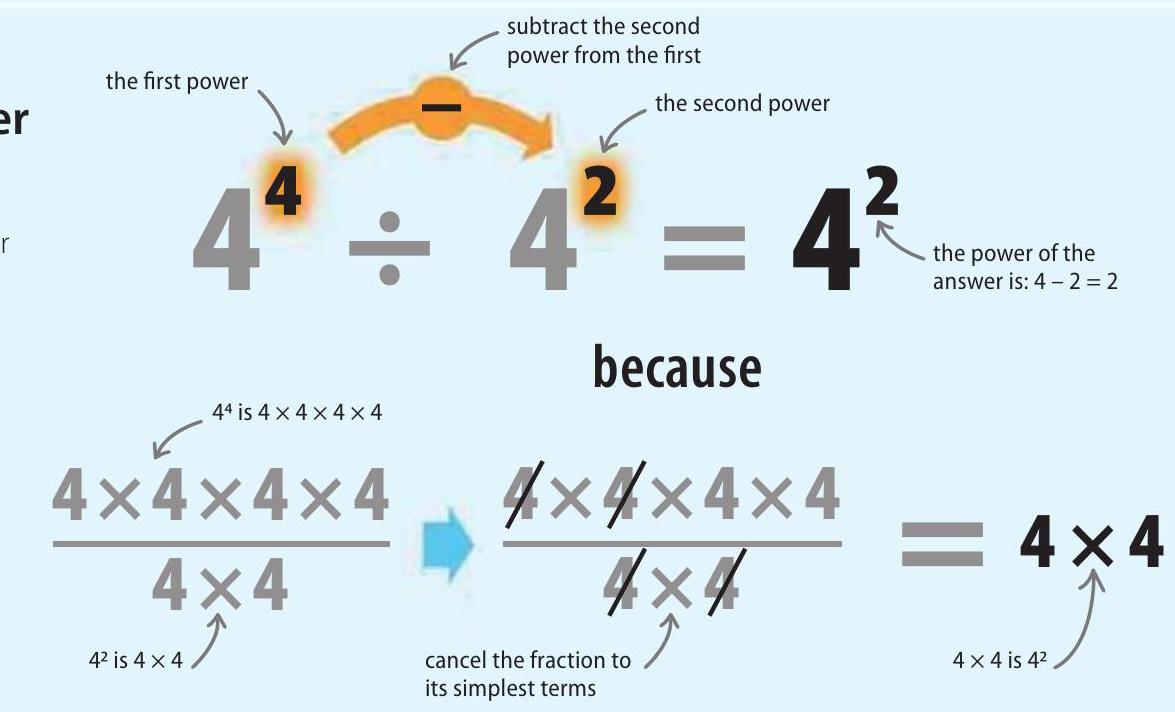
\includegraphics[max width=\textwidth, center]{2025_07_08_04014fa2c17a4b6cdcc6g-040(4)}

\section*{- Writing it out}
Writing out the division of the powers as a fraction and then cancelling the fraction shows why powers to be divided can simply be subtracted.

\section*{LOOKING CLOSER}
\section*{Zero power}
Any number raised to the power 0 is equal to 1 . Dividing two equal powers of the same number gives a power of 0 , and therefore the answer 1. These rules only apply when dealing with powers of the same number.\\
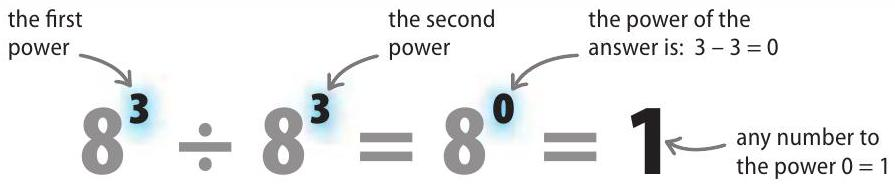
\includegraphics[max width=\textwidth, center]{2025_07_08_04014fa2c17a4b6cdcc6g-040(2)}\\
because

\section*{- Writing it out}
Writing out the division of two equal powers makes it clear why any number to the power 0 is always equal to 1 .\\
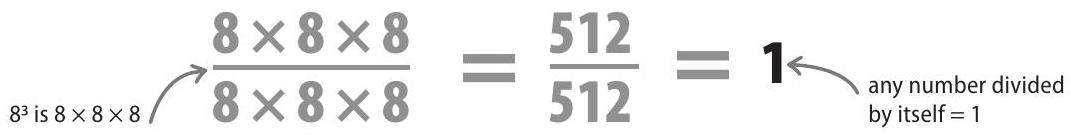
\includegraphics[max width=\textwidth, center]{2025_07_08_04014fa2c17a4b6cdcc6g-040}

\section*{Finding a square root by estimation}
It is possible to find a square root through estimation, by choosing a number to multiply by itself, working out the answer, and then altering the number depending on whether the answer needs to be higher or lower.\\
$\sqrt{32}=$ ?\\
$\sqrt{\mathbf{2 5}}=\mathbf{5}$ and $\sqrt{\mathbf{3 6}}=\mathbf{6}$, so the answer must be somewhere between 5 and 6. Start with the midpoint between the two, 5.5:\\
$5.5 \times 5.5=30.25 \quad$ Too low\\
$5.75 \times 5.75=33.0625 \quad$ Too high\\
$5.65 \times 5.65=31.9225 \quad$ Too low\\
$5.66 \times 5.66=32.0356$\\
\$\textbackslash sum\_\{\textbackslash substack\{\text{the square root of} 32 \text{is} \\


\text{approximately} 5.66\}\} \textbackslash quad\$\begin{tabular}{l}
this would round \\
down to 32 \\
\end{tabular}

the square root of 1,000 is approximately 31.62

\section*{$1,000=$ ?}
$\sqrt{\mathbf{1 , 6 0 0}}=\mathbf{4 0}$ and $\sqrt{\mathbf{9 0 0}}=\mathbf{3 0}$, so the answer must be between 40 and $30.1,000$ is closer to 900 than 1,600 , so start with a number closer to 30 , such as 32 :\\
$32 \times 32=1,024$ Too high\\
$31 \times 31=961$ Too low\\
$31.5 \times 31.5=992.25$ Too low\\
$31.6 \times 31.6=998.56$ Too low\\
$31.65 \times 31.65=1,001.72 \rightleftharpoons$ Too high\\
$31.62 \times 31.62=999.8244$\\
this would round up to 1,000 as the nearest whole number

\section*{Finding a cube root by estimation}
Cube roots of numbers can also be estimated without a calculator. Use round numbers to start with, then use these answers to get closer to the final answer.\\
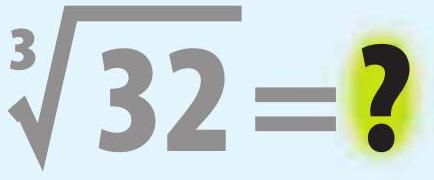
\includegraphics[max width=\textwidth, center]{2025_07_08_04014fa2c17a4b6cdcc6g-041}\\
$\mathbf{3} \times \mathbf{3} \times \mathbf{3}=\mathbf{2 7}$ and $\mathbf{4} \times \mathbf{4} \times \mathbf{4}=\mathbf{6 4}$, so the answer is somewhere between 3 and 4 . Start with the midpoint between the two, 3.5 :\\
$3.5 \times 3.5 \times 3.5=42.875$\\
$3.3 \times 3.3 \times 3.3=35.937$ Too high\\
$3.1 \times 3.1 \times 3.1=29.791$ Too high\\
$3.2 \times 3.2 \times 3.2=32.768$ Too high\\
$3.18 \times 3.18 \times 3.18=32.157432$

\footnotetext{The cube root of 32 is approximately 3.18
}
$\sqrt[3]{800}=$ ?\\
$\mathbf{9} \times \mathbf{9} \times \mathbf{9}=\mathbf{7 2 9}$ and $\mathbf{1 0} \times \mathbf{1 0} \times \mathbf{1 0}=\mathbf{1 , 0 0 0}$, so the answer is somewhere between 9 and 10.800 is closer to 729 than 1000, so start with a number closer to 9 , such as 9.1 :\\
$9.1 \times 9.1 \times 9.1=753.571$ Too low\\
$9.3 \times 9.3 \times 9.3=804.357$ Too high\\
$9.27 \times 9.27 \times 9.27=796.5979-$ Too low\\
$9.28 \times 9.28 \times 9.28=799.1787$ Very close\\
$9.284 \times 9.284 \times 9.284=800.2126$

\footnotetext{$\pi$ the cube root of 800 is approximately 9.284
}R\\
this would round down to 800

\section*{Surds}
A SURD IS A SQUARE ROOT THAT CANNOT BE WRITTEN\\
AS A WHOLE NUMBER. IT HAS AN INFINITE NUMBER OF DIGITS AFTER THE DECIMAL POINT.

\section*{Introducing surds}
Some square roots are whole numbers and are easy to write. But some are irrational numbers - numbers that go on forever after the decimal point. These numbers cannot be written out in full, so the most accurate way to express them is as square roots.

\section*{$\sqrt{5}=2.2360679774 \ldots$ \\
 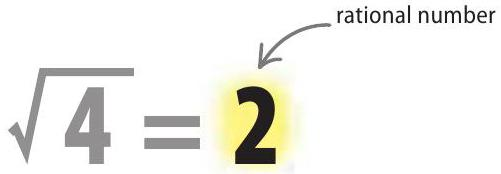
\includegraphics[max width=\textwidth]{2025_07_08_04014fa2c17a4b6cdcc6g-042}}
\section*{Surd}
The square root of 5 is an irrational number - it goes on forever. It cannot accurately be written out in full, so it is most simply expressed as the surd $\sqrt{ } 5$.

\section*{$\triangle$ Not a surd}
The square root of 4 is not a surd. It is the number 2, a whole, or rational number.

\section*{Simplifying surds}
Some surds can be made simpler by taking out factors that can be written as whole numbers. A few simple rules can help with this.

\section*{Square roots}
A square root is the number that, when multiplied by itself, gives the number inside the root.

\section*{$\sqrt{3} \times \sqrt{3}=3$}
multiply the surd by itself to give the number inside the square root

\section*{$\sqrt{a} \times \sqrt{a}=a$}
\begin{center}

\includegraphics[max width=\textwidth]{2025_07_08_04014fa2c17a4b6cdcc6g-042(3)}
\end{center}

\section*{- Multiplying roots}
Multiplying two numbers together and taking the square root of the result gives the same answer as taking the square roots of the two numbers and mutiplying them together.

$$
\sqrt{a b}=\sqrt{a} \times \sqrt{b}
$$

\begin{center}
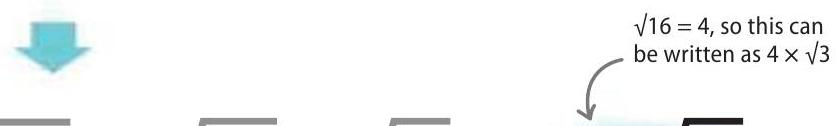
\includegraphics[max width=\textwidth]{2025_07_08_04014fa2c17a4b6cdcc6g-042(1)}
\end{center}

$$
\sqrt{48}=\sqrt{16 \times 3}=\sqrt{16} \times \sqrt{3}=4 \times \sqrt{3}
$$

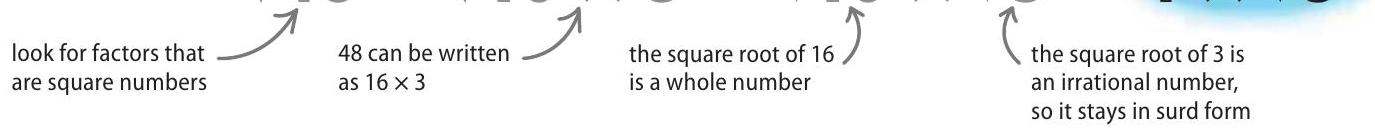
\includegraphics[max width=\textwidth, center]{2025_07_08_04014fa2c17a4b6cdcc6g-042(2)}\\
$\triangleright$ Dividing roots\\
Dividing one number by another and taking the square root of the result is the same as dividing the square root of the first number by the square root of the second.

$$
\sqrt{\frac{\mathrm{a}}{\mathrm{~b}}}=\frac{\sqrt{\mathrm{a}}}{\sqrt{\mathrm{~b}}} \Rightarrow \sqrt{\frac{7}{16}}=\frac{\sqrt{7}}{\sqrt{16}}=\frac{\sqrt{7}}{4}
$$

$\checkmark$ Simplifying further\\
When dividing square roots, look out for ways to simplify the top as well as the bottom of the fraction.

$$
\begin{aligned}
& \sqrt{\frac{8}{9}}=\frac{\sqrt{8}}{\sqrt{9}}=\frac{\sqrt{8}}{3} \int^{j^{13 \times 3}=9}=\left[\frac{2 \times \sqrt{2}}{3}\right. \\
& \sqrt{8}=\sqrt{4} \times \sqrt{2}=2 \times \sqrt{2} \\
& C_{814 \times 2}
\end{aligned}
$$

\section*{Surds in fractions}
When a surd appears in a fraction, it is helpful to make sure it appears in the numerator (top of the fraction) not the denominator (bottom of the fraction). This is called rationalizing, and is done by multiplying the whole fraction by the surd on the bottom.

\begin{itemize}
  \item Rationalizing
\end{itemize}

The fraction stays the same if the top and bottom are multiplied by the same number.

\section*{$\triangleright$ Simplifying further}
Sometimes rationalizing a fraction gives us another surd that can be simplified further.

$$
\frac{12}{\sqrt{15}}=\frac{12 \times \sqrt{15}}{\sqrt{15} \times \sqrt{15}}=
$$

\begin{center}
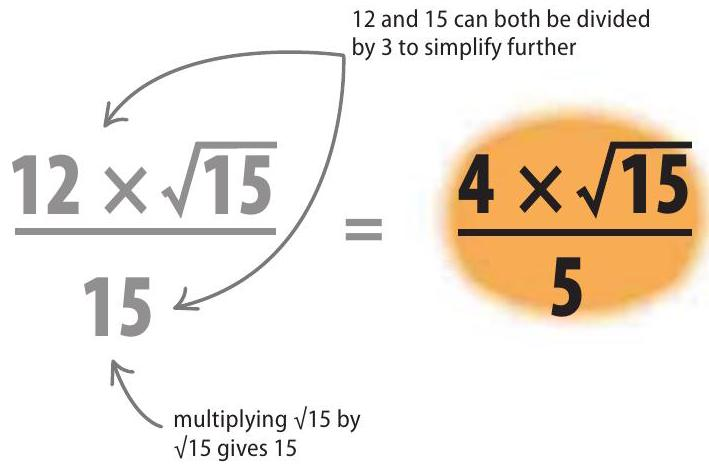
\includegraphics[max width=\textwidth]{2025_07_08_04014fa2c17a4b6cdcc6g-043}
\end{center}

\section*{$4 \times 10^{\circ}$ Standard Form}
\section*{STANDARD FORM IS A CONVENIENT WAY OF WRITING VERY LARGE AND VERY SMALL NUMBERS.}
\begin{center}
\begin{tabular}{|l|}
\hline
SEE ALSO \\
\hline
《18-21 Multiplication \\
\hline
22-25 Division \\
\hline
36-39 Powers and roots \\
\hline
\end{tabular}
\end{center}

\section*{Introducing standard form}
Standard form makes very large or very small numbers easier to understand by showing them as a number multiplied by a power of 10. This is useful because the size of the power of 10 makes it possible to get an instant impression of how big the number really is.\\
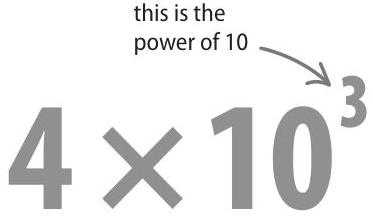
\includegraphics[max width=\textwidth, center]{2025_07_08_04014fa2c17a4b6cdcc6g-044(4)}\\
$\triangleleft$ Using standard form This is how 4,000 is written as standard form - it shows that the decimal place for the number represented, 4,000, is 3 places to the right of 4.

\section*{How to write a number in standard form}
To write a number in standard form, work out how many places the decimal point must move to form a number between 1 and 10. If the number does not have a decimal point, add one after its final digit.

\section*{Take a number}
Standard form is usually used for very large or very small numbers.\\
$\triangleright$ Add the decimal point Identify the position of the decimal point if there is one. Add a decimal point at the end of the number, if it does not already have one.

\section*{- Move the decimal point}
Move along the number and count how many places the decimal point must move to form a number between 1 and 10.

\section*{- Write as standard form}
The number between 1 and 10 is multiplied by 10 , and the small number, the "power" of 10 , is found by counting how many places the decimal point moved to create the first number.\\
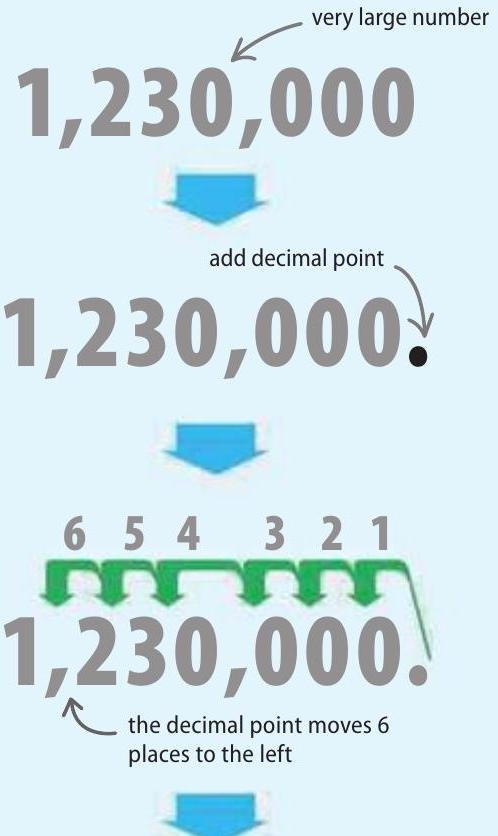
\includegraphics[max width=\textwidth, center]{2025_07_08_04014fa2c17a4b6cdcc6g-044(3)}\\
the power is 6 because the decimal point moved six places; the power is positive because the decimal point moved to the left\\
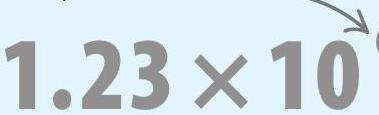
\includegraphics[max width=\textwidth, center]{2025_07_08_04014fa2c17a4b6cdcc6g-044(1)}\\
the first number must always be between 1 and 10\\
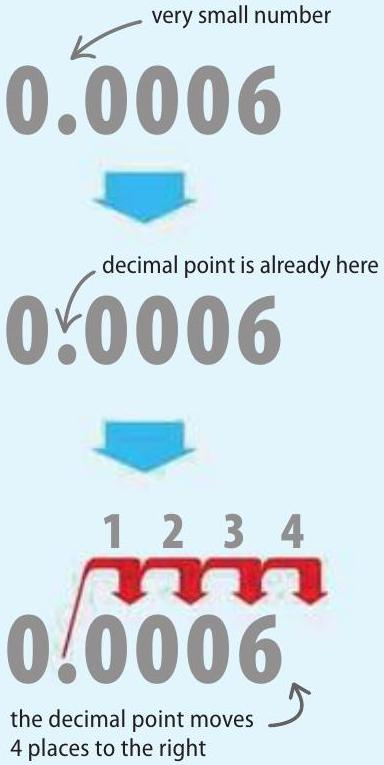
\includegraphics[max width=\textwidth, center]{2025_07_08_04014fa2c17a4b6cdcc6g-044(2)}\\
the power is negative because the decimal point moved to the right\\
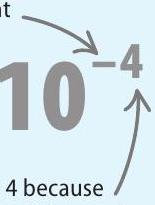
\includegraphics[max width=\textwidth, center]{2025_07_08_04014fa2c17a4b6cdcc6g-044}\\
the power is 4 because the decimal point moved four places

\section*{Standard form in action}
Sometimes it is difficult to compare how large or small numbers are because of the number of digits they contain. Standard form makes this easier.

The mass of Earth is $5,974,200,000,000,000,000,000,000 \mathrm{~kg}$

$$
\begin{aligned}
& 242322212019181716151413121110198776514321 \\
& \text { montriting merrorm } \\
& 5,974,200,000,000,000,000,000,000.0 \mathrm{~kg}
\end{aligned}
$$

The decimal point moves 24 places to the left.

The mass of the planet Mars is

\section*{$2322212019181716151413121110 \quad 9 \quad 8 \quad 7 \quad 6 \quad 5 \quad 4 \quad 3 \quad 21$ пеイ519TSTITYTITITYTIT 641,910,000,000,000,000,000,000.0 kg}
\begin{center}
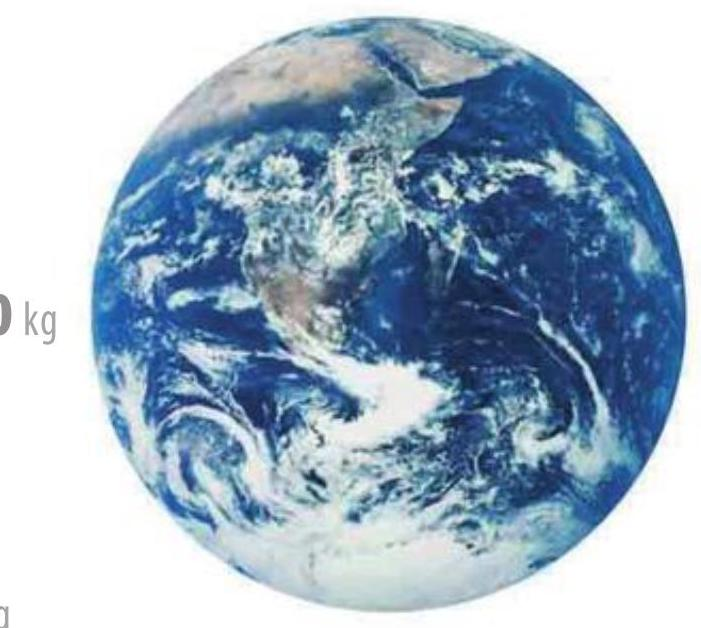
\includegraphics[max width=\textwidth]{2025_07_08_04014fa2c17a4b6cdcc6g-045(2)}
\end{center}

The decimal point moves $\mathbf{2 3}$ places to the left.

Written in standard form these numbers are much easier to compare. Earth's mass in standard form is

$$
5.9742 \times 10^{24} \mathrm{~kg}
$$

The mass of Mars in standard form is

$$
6.4191 \times 10^{23} \mathrm{~kg}
$$

\begin{center}
\begin{tabular}{|l|l|l|}
\hline
\multicolumn{3}{|c|}{EXAMPLES OF STANDARD FORM} \\
\hline
Example & Decimal form & Standard form \\
\hline
Weight of the Moon & $73,600,000,000,000,000,000,000 \mathrm{~kg}$ & $7.36 \times 10^{22} \mathrm{~kg}$ \\
\hline
Humans on Earth & 6,800,000,000 & $6.8 \times 10^{9}$ \\
\hline
Speed of light & $300,000,000 \mathrm{~m} / \mathrm{sec}$ & $3 \times 10^{8} \mathrm{~m} / \mathrm{sec}$ \\
\hline
Distance of the Moon from the Earth & $384,000 \mathrm{~km}$ & $3.8 \times 10^{5} \mathrm{~km}$ \\
\hline
Weight of the Empire State building & 365,000 tons & $3.65 \times 10^{5}$ tons \\
\hline
Distance around the Equator & $40,075 \mathrm{~km}$ & $4 \times 10^{4} \mathrm{~km}$ \\
\hline
Height of Mount Everest & $8,850 \mathrm{~m}$ & $8.850 \times 10^{3} \mathrm{~m}$ \\
\hline
Speed of a bullet & $710 \mathrm{~m} / \mathrm{sec}$ & $7.1 \times 10^{2} \mathrm{~m} / \mathrm{sec}$ \\
\hline
Speed of a snail & $0.001 \mathrm{~m} / \mathrm{sec}$ & $1 \times 10^{-3} \mathrm{~m} / \mathrm{sec}$ \\
\hline
Width of a red blood cell & 0.00067 cm & $6.7 \times 10^{-4} \mathrm{~cm}$ \\
\hline
Length of a virus & 0.000000009 cm & $9 \times 10^{-9} \mathrm{~cm}$ \\
\hline
Weight of a dust particle & 0.000000000753 kg & $7.53 \times 10^{-10} \mathrm{~kg}$ \\
\hline
\end{tabular}
\end{center}

$\triangleright$ Comparing planet mass\\
It is immediately evident that the mass of the Earth is bigger than the mass of Mars, as $10^{24}$ is 10 times\\
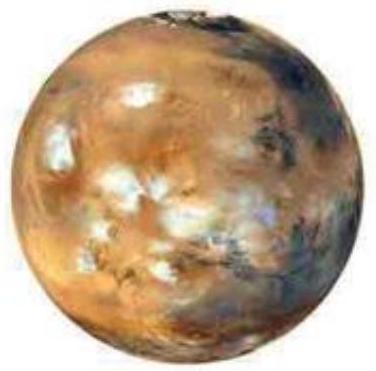
\includegraphics[max width=\textwidth]{2025_07_08_04014fa2c17a4b6cdcc6g-045(1)} larger than $10^{23}$.

\section*{LOOKING CLOSER}
\section*{Standard form and calculators}
The exponent button on a calculator allows a number to be raised to any power. Calculators give very large answers in standard form.

\section*{$\mathrm{X}^{\mathrm{y}}$}
$\triangle$ Exponent button This calculator button allows any number to be raised to any power.

Using the exponent button:\\
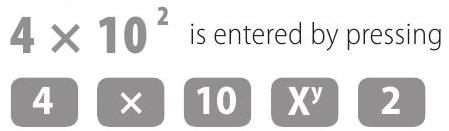
\includegraphics[max width=\textwidth, center]{2025_07_08_04014fa2c17a4b6cdcc6g-045}

On some calculators, answers appear in standard form:

$$
\begin{aligned}
& 1234567 \times 89101112= \\
& 1.100012925 \times 10^{14}= \\
& \text { so the answer is approximately } \\
& 110,001,292,500,000
\end{aligned}
$$

\section*{Decimals}
\section*{NUMBERS WRITTEN IN DECIMAL FORM ARE CALLED DECIMAL NUMBERS OR, MORE SIMPLY, DECIMALS.}
\begin{center}
\begin{tabular}{|l|}
\hline
SEE ALSO \\
\hline
《18-21 Multiplication \\
\hline
《22-25 Division \\
\hline
\begin{tabular}{l}
Using a \\
calculator \\
\end{tabular} \\
\hline
\end{tabular}
\end{center}

\section*{Decimal numbers}
In a decimal number, the digits to the left of the decimal point are whole numbers. The digits to the right of the decimal point are not whole numbers. The first digit to the right of the decimal point represents tenths, the second hundredths, and so on. These are called fractional parts.\\
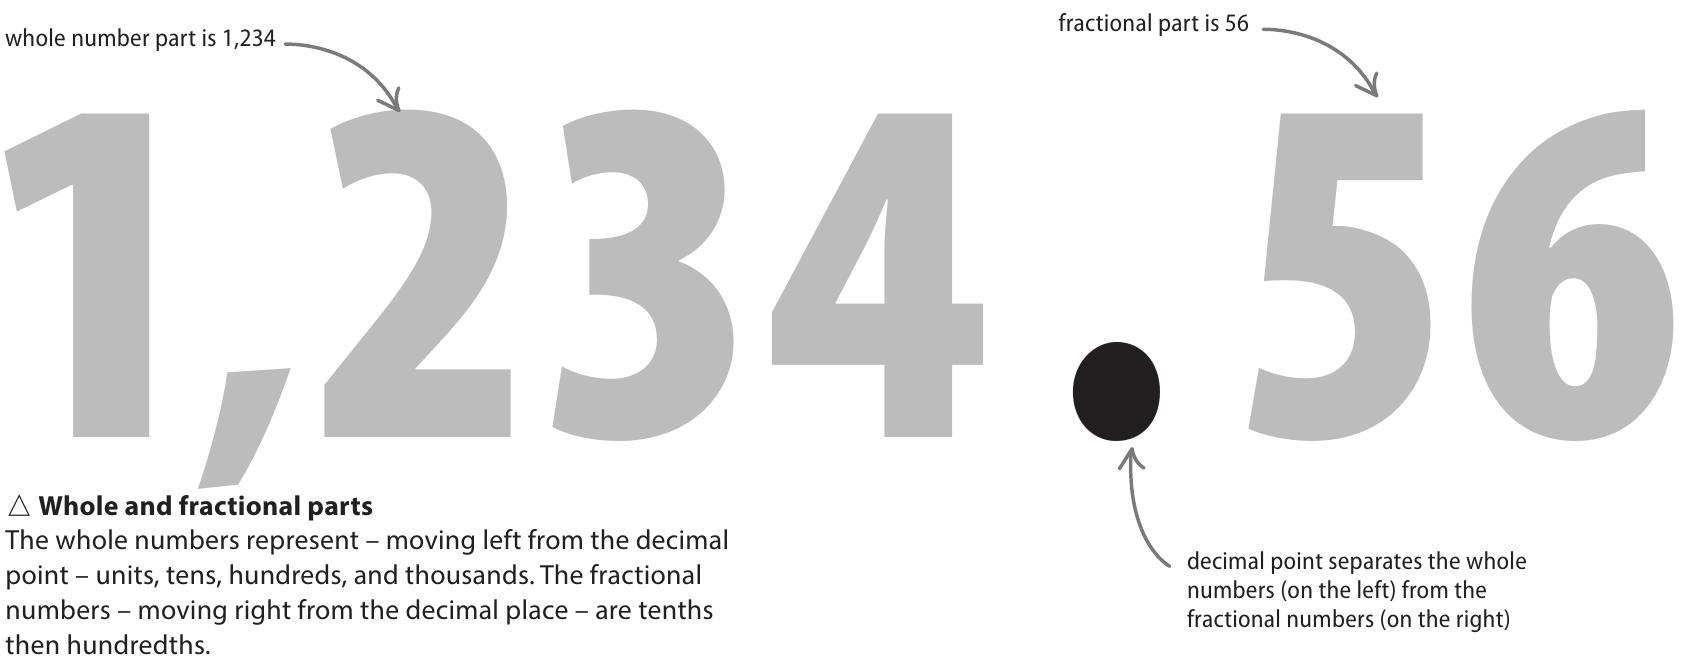
\includegraphics[max width=\textwidth, center]{2025_07_08_04014fa2c17a4b6cdcc6g-046(2)}

\section*{Multiplication}
To multiply decimals, first remove the decimal point. Then perform a long multiplication of the two numbers, before adding the decimal point back in to the answer. Here 1.9 (a decimal) is multiplied by 7 (a whole number).\\
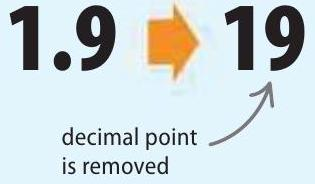
\includegraphics[max width=\textwidth, center]{2025_07_08_04014fa2c17a4b6cdcc6g-046(1)}

First, remove any decimal points, so that both numbers can be treated as whole numbers.\\
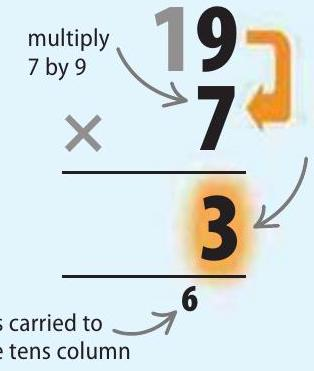
\includegraphics[max width=\textwidth, center]{2025_07_08_04014fa2c17a4b6cdcc6g-046}

Then multiply the two numbers, starting in the units column. Carry units to the tens if necessary.

Next multiply the tens. The product is 7, which, added to the carried 6, makes 13. Write this across two columns.

Finally, count the decimal digits in the original numbers there is 1 . The answer will also have 1 decimal digit.

\section*{DIVISION}
Dividing one number by another often gives a decimal answer. Sometimes it is easier to turn decimals into whole numbers before dividing them.

\section*{Short division with decimals}
Many numbers do not divide into each other exactly. If this is the case, a decimal point is added to the number being divided, and zeros are added after the point until the division is solved. Here 6 is divided by 8.

Both numbers are whole. As 8 will not divide into 6, put in a decimal point with a 0 after it and carry the 6.\\
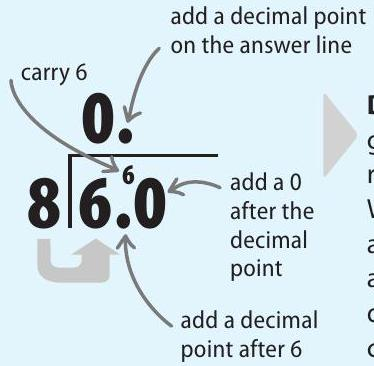
\includegraphics[max width=\textwidth, center]{2025_07_08_04014fa2c17a4b6cdcc6g-047(4)}

\section*{Dividing decimals}
Above, short division was used to find the decimal answer for the sum $8 \div 6$. Long division can be used to achieve the same result.\\
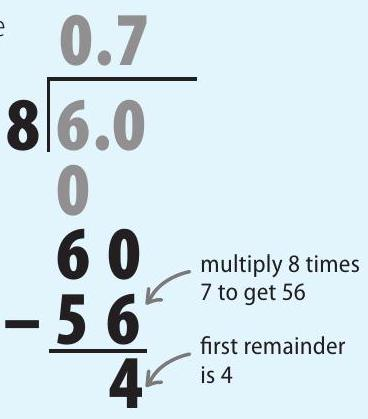
\includegraphics[max width=\textwidth, center]{2025_07_08_04014fa2c17a4b6cdcc6g-047(7)}

Work out the first remainder by multiplying 8 by 7 and subtracting this from 60. The answer is 4.\\
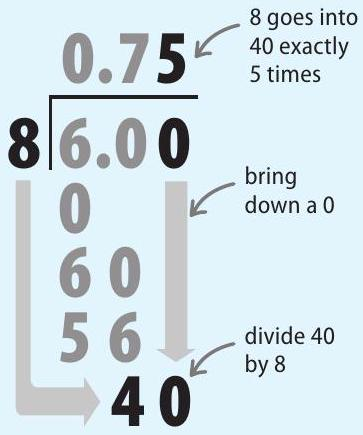
\includegraphics[max width=\textwidth, center]{2025_07_08_04014fa2c17a4b6cdcc6g-047(2)}

Bring down a zero to join the 4 and divide the number by 8 . It goes exactly 5 times, so put a 5 above the line.\\
Bring down a zero to join by 8 . It goes exactly 5 time\\
so put a 5 above the line.

\section*{LOOKING CLOSER}
\section*{Decimals that do not end}
Sometimes the answer to a division can be a decimal number that repeats without ending. This is called a "recurring" decimal. For example, here 1 is divided by 3 . Both the calculations and the answers in the division become identical after the second stage, and the answer recurs endlessly.\\
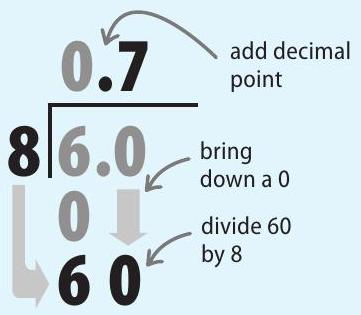
\includegraphics[max width=\textwidth, center]{2025_07_08_04014fa2c17a4b6cdcc6g-047(3)}

Subtract 0 from 6 to get 6, and bring down a 0 . Divide 8 into 60 and put the answer, 7, after a decimal point.\\
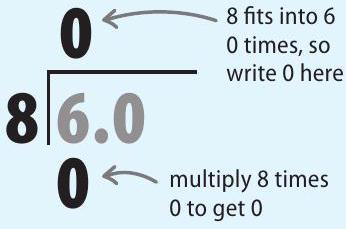
\includegraphics[max width=\textwidth, center]{2025_07_08_04014fa2c17a4b6cdcc6g-047(1)}

First, divide 8 into 6. It goes 0 times, so put a 0 above the 6 . Multiply $8 \times 0$, and write the result ( 0 ) under the 6 .\\
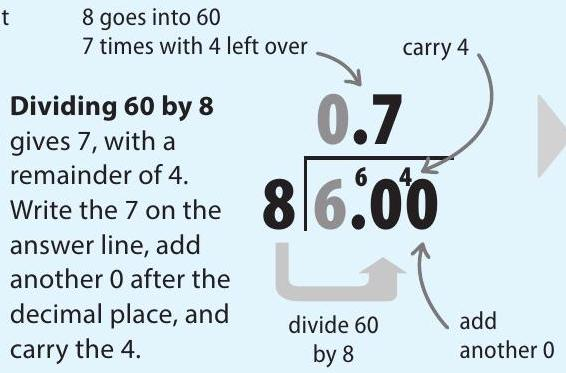
\includegraphics[max width=\textwidth, center]{2025_07_08_04014fa2c17a4b6cdcc6g-047(6)}\\
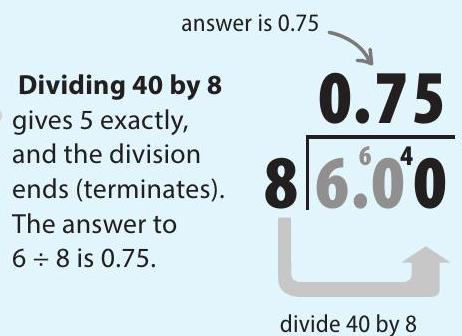
\includegraphics[max width=\textwidth, center]{2025_07_08_04014fa2c17a4b6cdcc6g-047(5)}\\
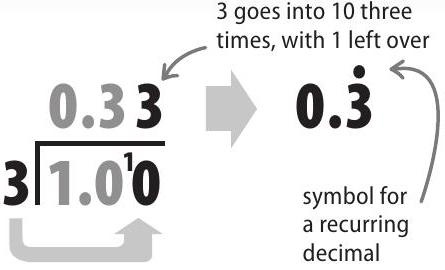
\includegraphics[max width=\textwidth, center]{2025_07_08_04014fa2c17a4b6cdcc6g-047}

Dividing 10 by 3 again gives exactly the same answer as the last step. This is repeated infinitely. This type of recurring decimal is written with a dot over the recurring digit.

\section*{10101}
\section*{Binary numbers}
NUMBERS ARE COMMONLY WRITTEN USING THE DECIMAL

\begin{center}
\begin{tabular}{|l|}
\hline
SEE ALSO \\
\hline
《14-15 Introducing numbers \\
\hline
《33 Roman numerals \\
\hline
\end{tabular}
\end{center} SYSTEM, BUT NUMBERS CAN BE WRITTEN IN ANY NUMBER BASE.

\section*{What is a binary number?}
The decimal system uses the digits 0 through to 9 , while the binary system, also known as base 2, uses only two digits -0 and 1 . Binary numbers should not be thought of in the same way as decimal numbers. For example, 10 is said as "ten" in the decimal system but must be said as "one zero" in the binary system. This is because the value of each "place" is different in decimal and binary.

\section*{Counting in the decimal system}
When using the decimal system for column sums, numbers are written from right to left (from lowest to highest). Each column is worth ten times more than the column to the right of it. The decimal number system is also known as base 10.\\
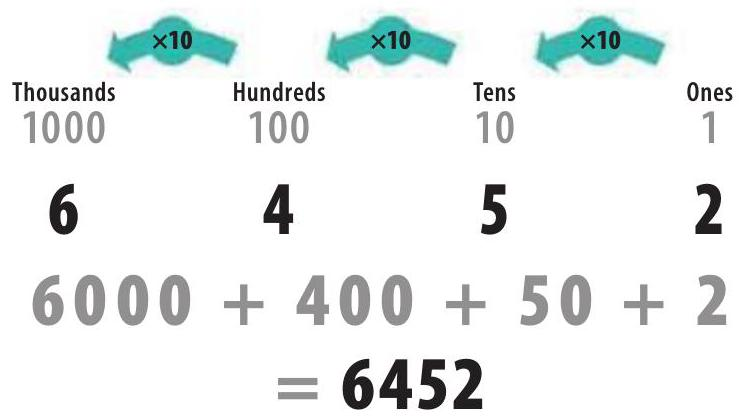
\includegraphics[max width=\textwidth, center]{2025_07_08_04014fa2c17a4b6cdcc6g-048}

\section*{Counting in binary}
Each column in the binary system is worth two times more than the column to the right of it and, as in the decimal system, 0 represents zero value. A similar system of headings may be used with binary numbers but only two symbols are used (0 and 1).\\
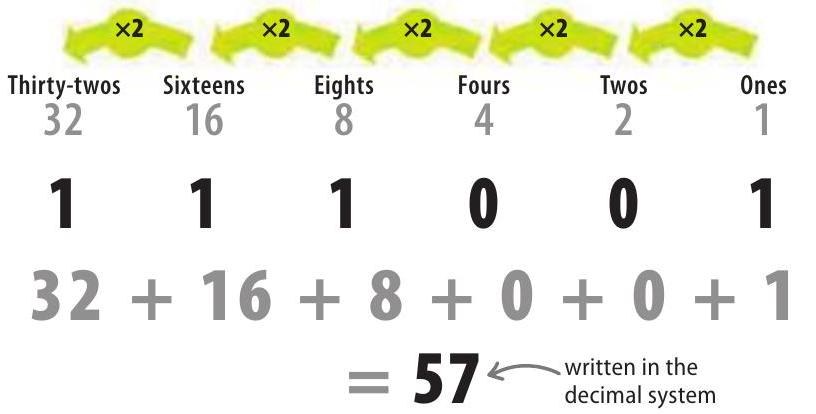
\includegraphics[max width=\textwidth, center]{2025_07_08_04014fa2c17a4b6cdcc6g-048(1)}

Decimal numbers

\section*{01123456789}
\section*{Binary numbers}
$01 \longleftarrow \begin{aligned} & \text { a single binary digit is } \\ & \text { called a "bit", which is } \\ & \text { a }\end{aligned}$ short for binary digit

\begin{center}
\begin{tabular}{|l|l|l|}
\hline
Decimal & \multicolumn{2}{|l|}{Binary} \\
\hline
0 & \multicolumn{2}{|c|}{\begin{tabular}{l}
0 \\
0 \\
\end{tabular}} \\
\hline
1 & 1 & 1 one \\
\hline
2 & 10 & 1 two \\
\hline
3 & 11 & 1 two + 1 one \\
\hline
4 & 100 & 1 four \\
\hline
5 & 101 & 1 four + 1 one \\
\hline
6 & 110 & 1 four + 1 two \\
\hline
7 & 111 & 1 four + 1 two + 1 one \\
\hline
8 & 1000 & 1 eight \\
\hline
9 & 1001 & 1 eight + 1 one \\
\hline
10 & 1010 & 1 eight + 1 two \\
\hline
11 & 1011 & 1 eight + 1 two + 1 one \\
\hline
12 & 1100 & 1 eight +1 four \\
\hline
13 & 1101 & 1 eight +1 four +1 one \\
\hline
14 & 1110 & 1 eight +1 four +1 two \\
\hline
15 & 1111 & 1 eight +1 four +1 two + 1 one \\
\hline
16 & 10 & 1 sixteen \\
\hline
17 & 10 & 1 sixteen + 1 one \\
\hline
18 & 10 & 1 sixteen + 1 two \\
\hline
19 & 10 & 1 sixteen + 1 two + 1 one \\
\hline
20 & 10 & 1 sixteen + 1 four \\
\hline
50 & 110 & 1 thirty-two + 1 sixteen + 1 two \\
\hline
100 & 1100 & 1 sixty-four + 1 thirty-two + 1 four \\
\hline
\end{tabular}
\end{center}

\section*{Adding in binary}
Numbers written in binary form can be added together in a similar way to decimal numbers, and column addition may be done like this:\\
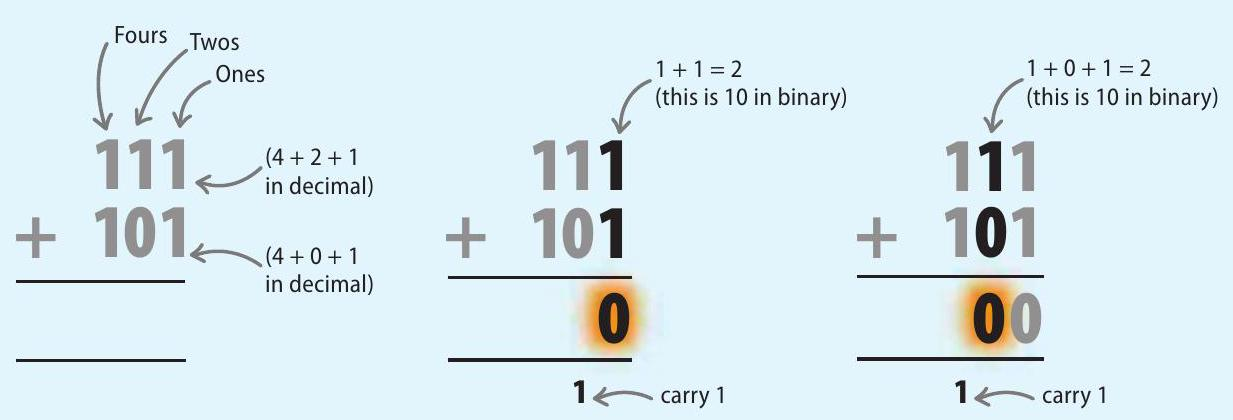
\includegraphics[max width=\textwidth, center]{2025_07_08_04014fa2c17a4b6cdcc6g-049(4)}

Align the numbers\\
under their correct place-value columns as in the decimal system. It may be helpful to write in the column headings when first learning this system.

\section*{Add the ones column.}
The answer is 2 , which is 10 in binary. The twos are shown in the next column so carry a 1 to the next column and leave 0 in the ones column.

Now the digits in the twos column are added together with the 1 carried over from the ones column. The total is 2 again ( 10 in binary) so a 1 needs to be carried and a 0 left in the twos column.\\
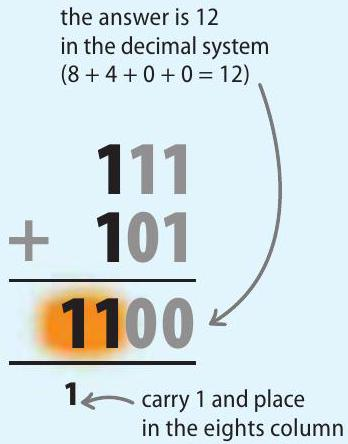
\includegraphics[max width=\textwidth, center]{2025_07_08_04014fa2c17a4b6cdcc6g-049(3)}

Finally, add the 1s in the fours column, which gives us 3 , ( 11 in binary). This is the end of the sum so the final 1 is placed in the eights column.

\section*{Subtracting in binary}
Subtraction works in a similar way to the decimal system but "borrows" in different units to the decimal system - borrowing by twos instead of tens.\\
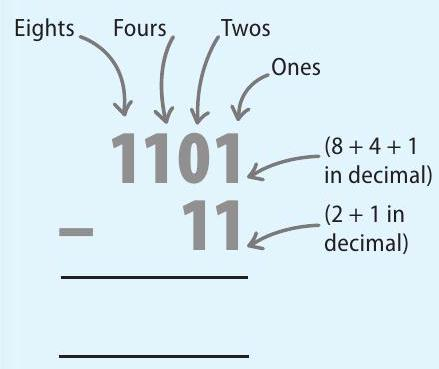
\includegraphics[max width=\textwidth, center]{2025_07_08_04014fa2c17a4b6cdcc6g-049}

The numbers are written in their correct place-value columns as in the decimal system.\\
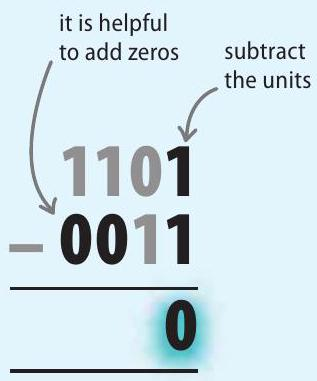
\includegraphics[max width=\textwidth, center]{2025_07_08_04014fa2c17a4b6cdcc6g-049(1)}

Add zeros so that there are the same number of digits in each column. Then begin by subtracting the ones column: 1 minus 1 is 0 , so place a 0 in the answer space. Now move on to the twos column on the left.\\
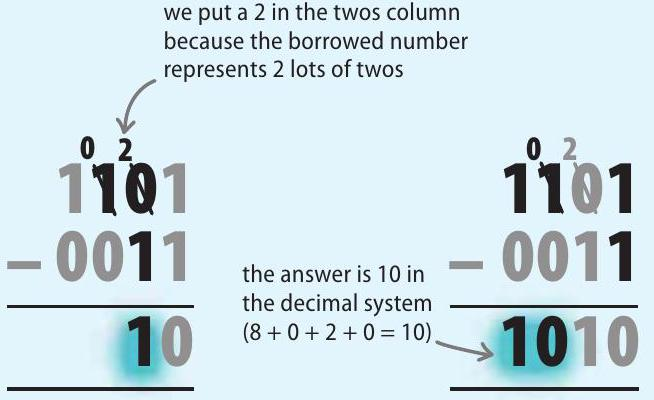
\includegraphics[max width=\textwidth, center]{2025_07_08_04014fa2c17a4b6cdcc6g-049(2)}

The lower 1 cannot be subtracted from the 0 above it so borrow from the fours column and replace it with a 0 . Then put a 2 above the twos column. Subtract the lower 1 from the upper 2. This leaves 1 as the answer.

Now subtract the digits in the fours column, which gives us 0 . Finally, in the eights column we have nothing to subtract from the upper 1 , so 1 is written in the answer space.

\section*{Fractions}
\section*{A FRACTION REPRESENTS A PART OF A WHOLE NUMBER. THEY ARE WRITTEN AS ONE NUMBER OVER ANOTHER NUMBER.}
\begin{center}
\begin{tabular}{|l|l|}
\hline
SEE ALSO &  \\
\hline
< 22-25 & Division \\
\hline
< 44-45 & Decimals \\
\hline
\begin{tabular}{l}
Ratio and \\
proportion \\
\end{tabular} & $\mathbf{5 6 - 5 9} \boldsymbol{)}$ \\
\hline
Percentages & $\mathbf{6 0 - 6 1} \boldsymbol{>}$ \\
\hline
\begin{tabular}{l}
Converting \\
fractions, decimals, \\
and percentages \\
\end{tabular} & $\mathbf{6 4 - 6 5} \boldsymbol{)}$ \\
\hline
\end{tabular}
\end{center}

\begin{center}
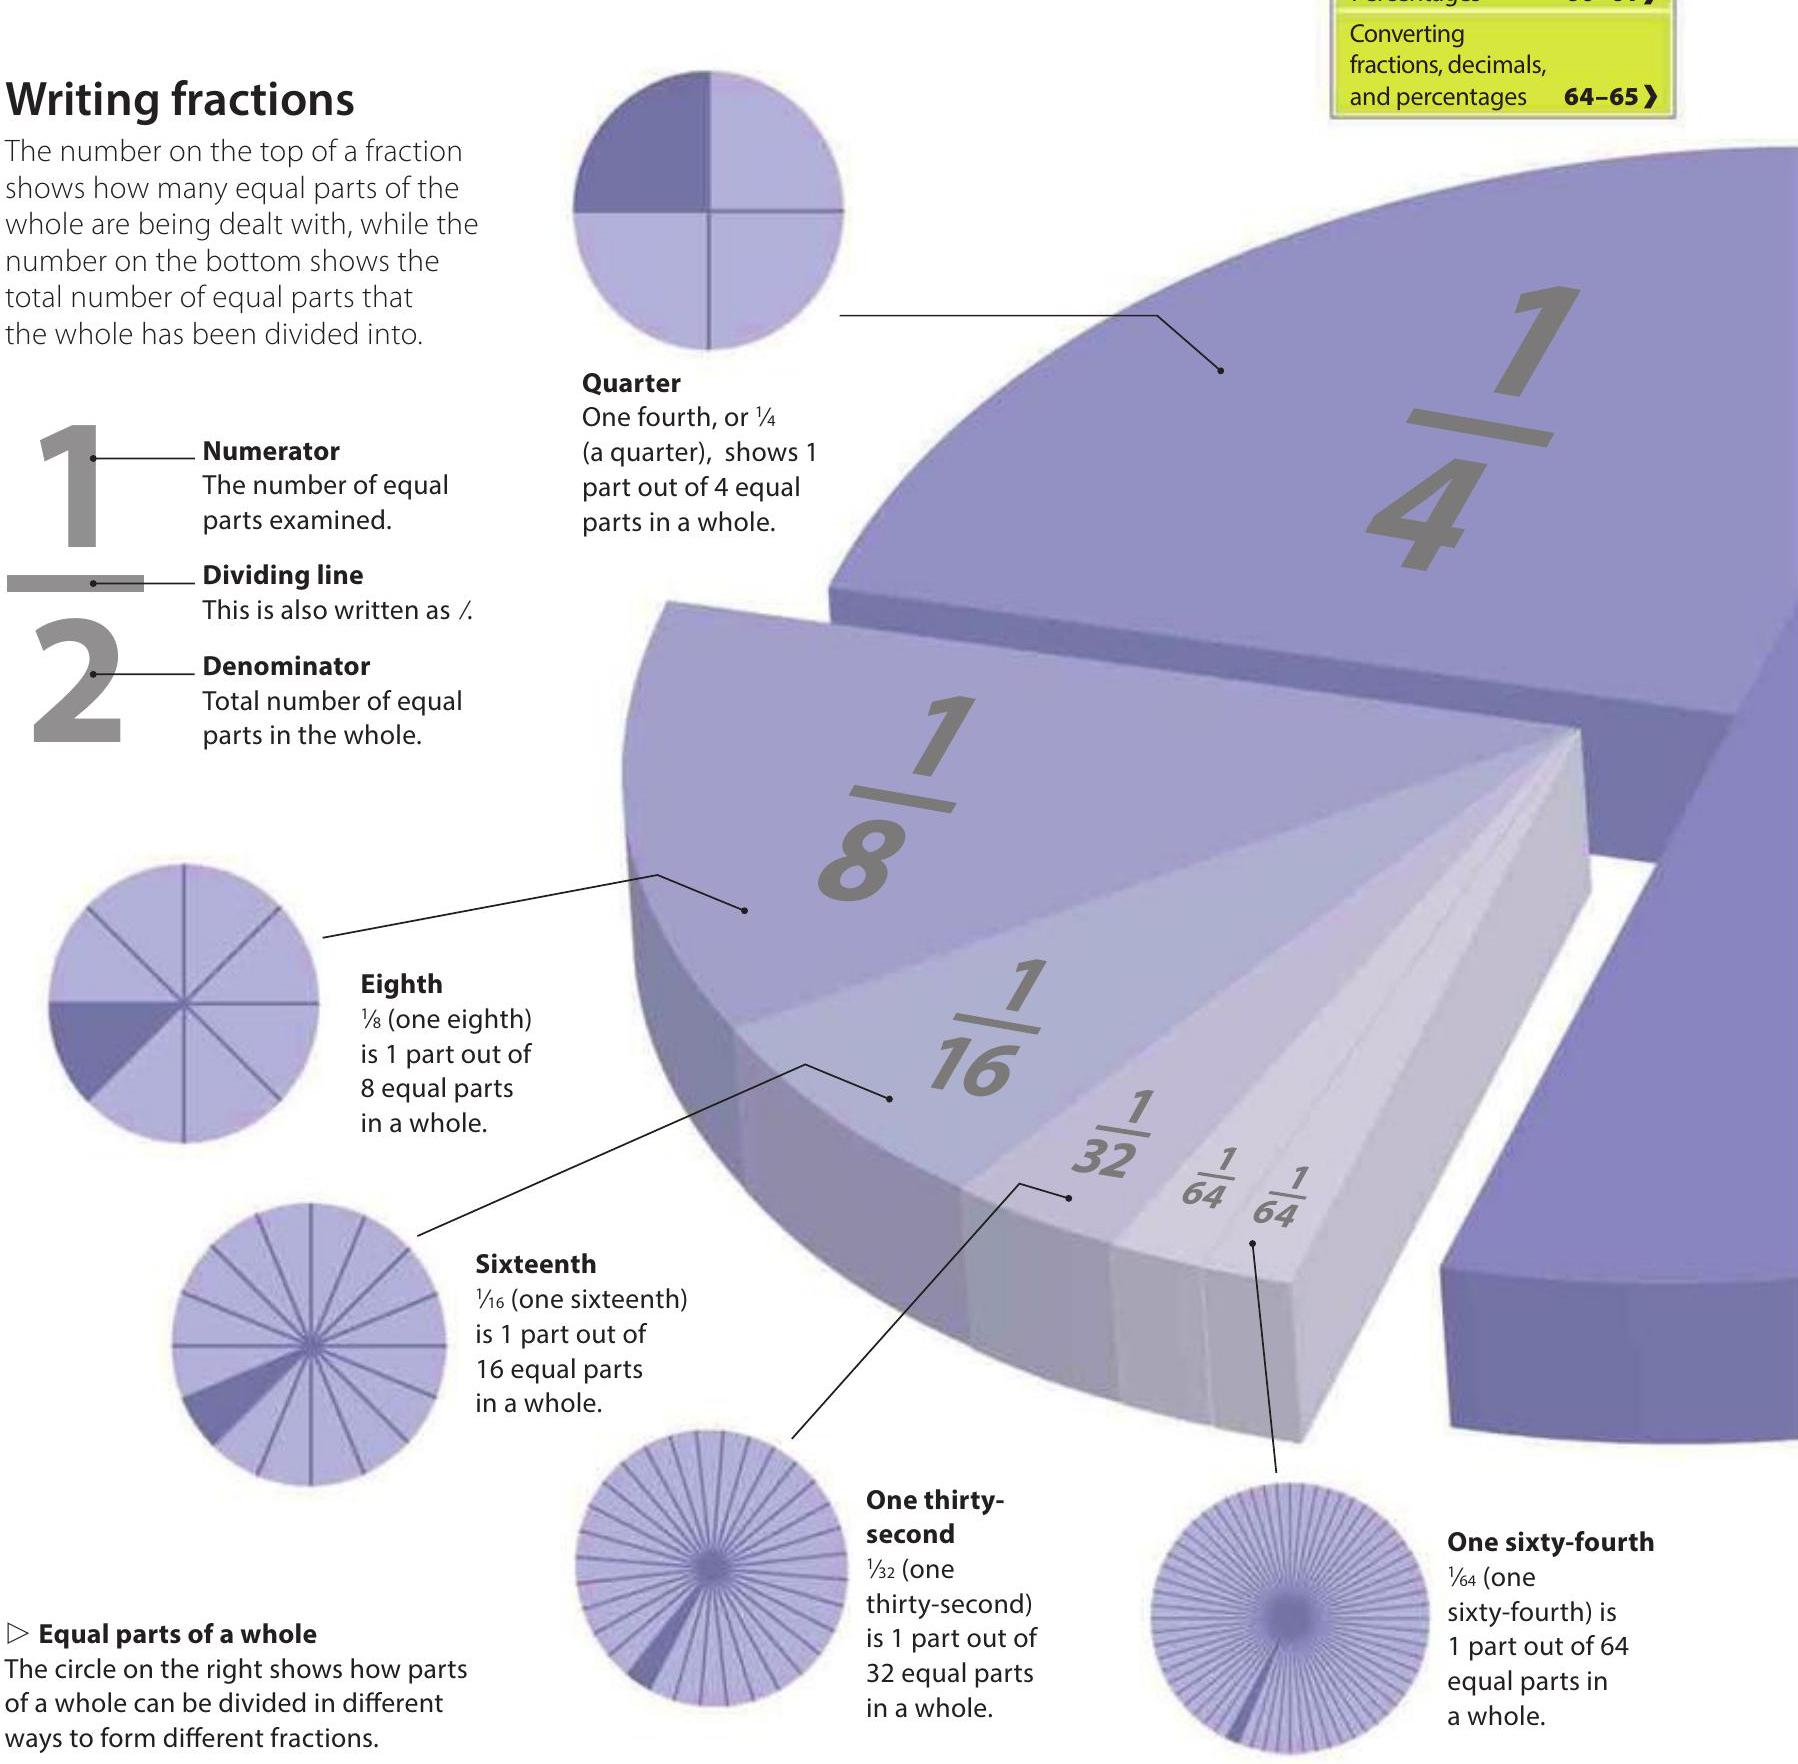
\includegraphics[max width=\textwidth]{2025_07_08_04014fa2c17a4b6cdcc6g-050}
\end{center}

\section*{Types of fractions}
A proper fraction - where the numerator is smaller than the denominator - is just one type of fraction. When the number of parts is greater than the whole, the result is a fraction that can be written in two ways - either as an improper fraction (also known as a top-heavy fraction) or a mixed fraction.\\
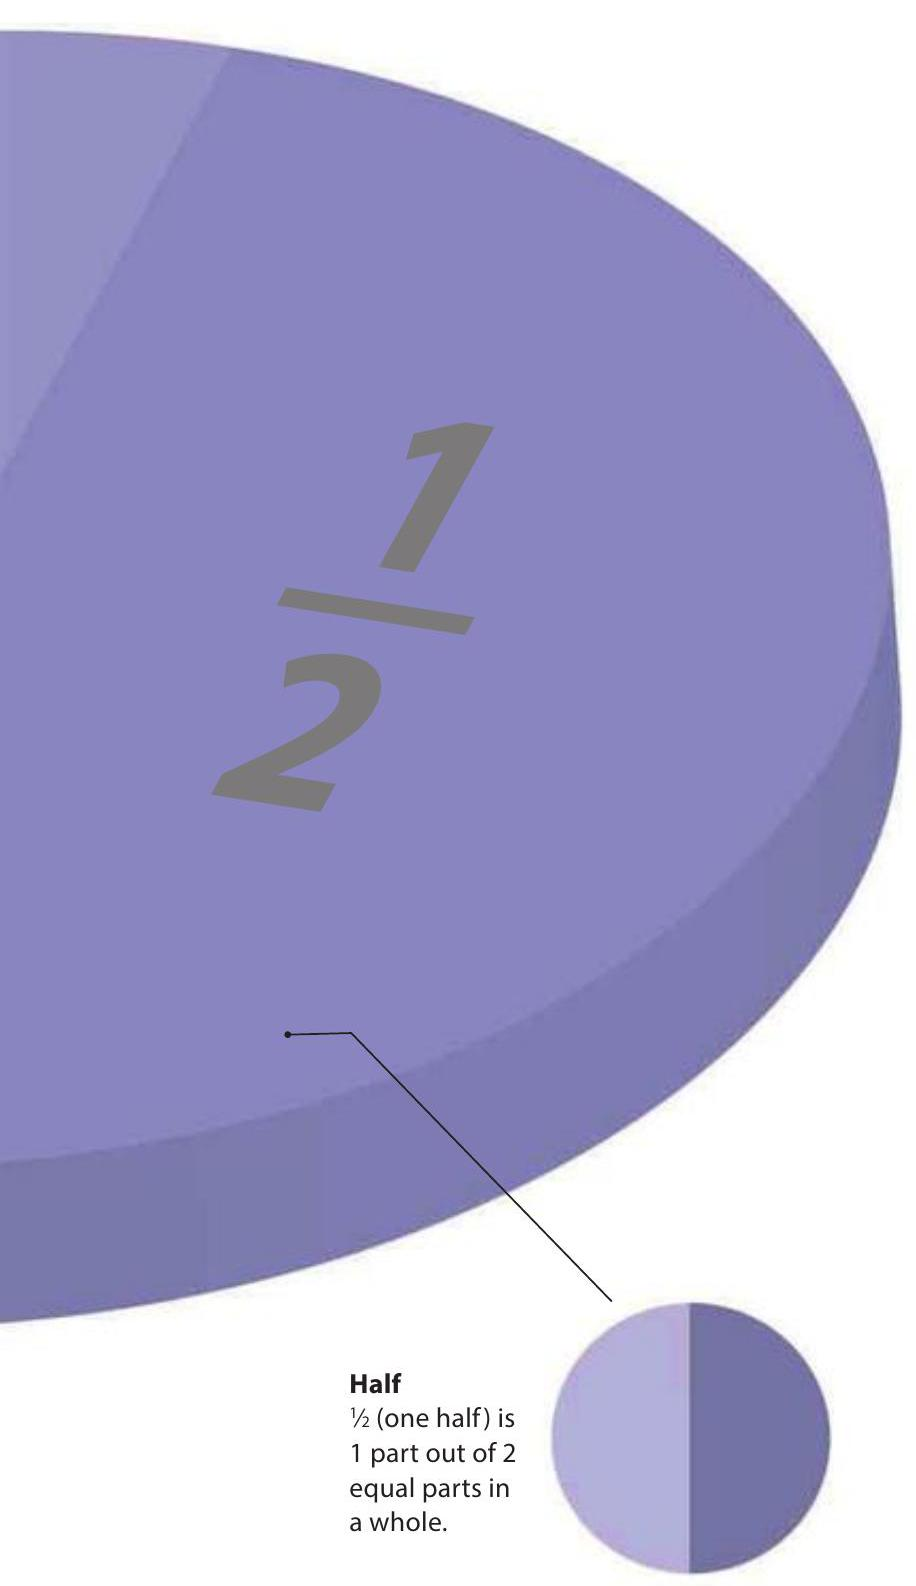
\includegraphics[max width=\textwidth, center]{2025_07_08_04014fa2c17a4b6cdcc6g-051(3)}\\
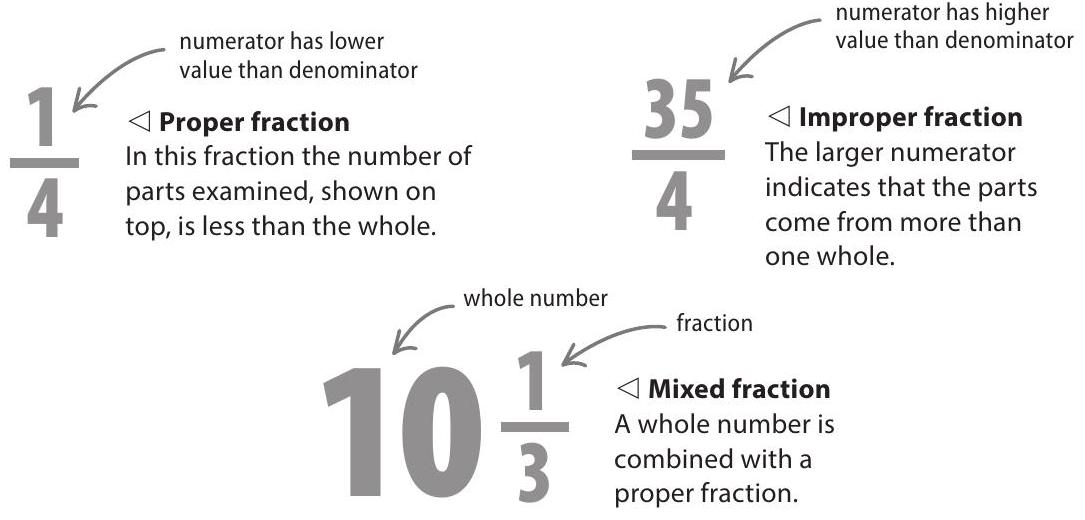
\includegraphics[max width=\textwidth, center]{2025_07_08_04014fa2c17a4b6cdcc6g-051(1)}

\section*{Depicting fractions}
Fractions can be illustrated in many ways, using any shape that can be divided into an equal number of parts.\\
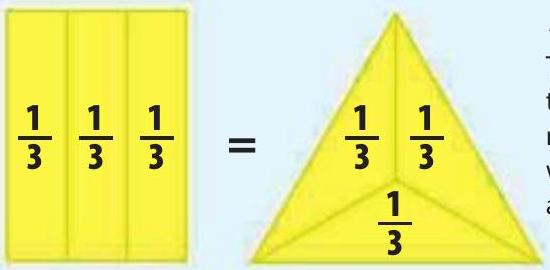
\includegraphics[max width=\textwidth, center]{2025_07_08_04014fa2c17a4b6cdcc6g-051}\\
$\triangleleft$ Split equally\\
The shapes show that there is more than one way of depicting a fraction.\\
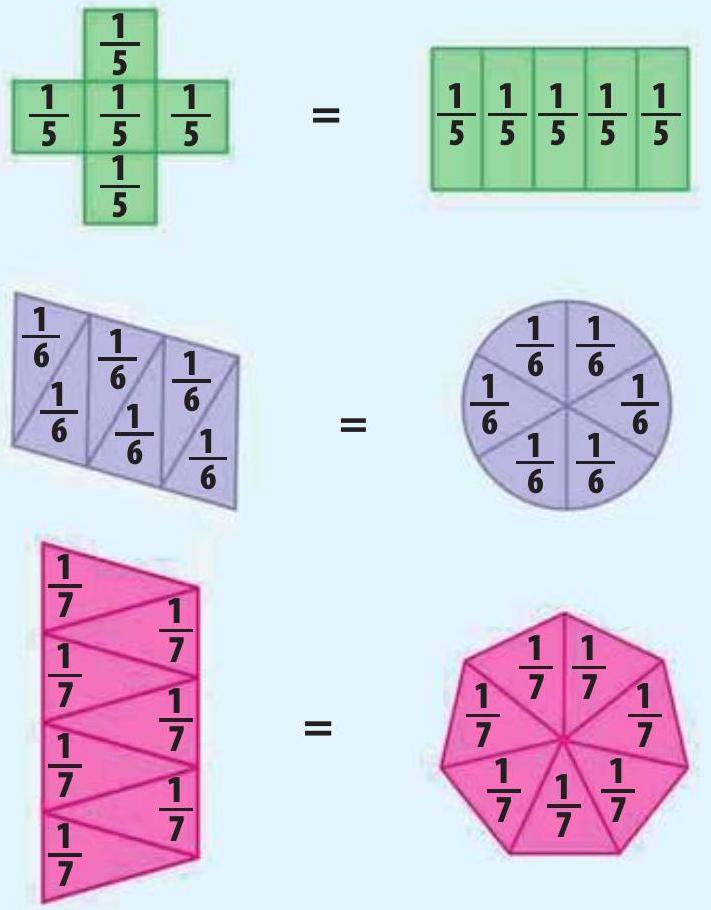
\includegraphics[max width=\textwidth, center]{2025_07_08_04014fa2c17a4b6cdcc6g-051(2)}

\section*{Turning top-heavy fractions into mixed fractions}
A top-heavy fraction can be turned into a mixed fraction by dividing the numerator by the denominator.\\
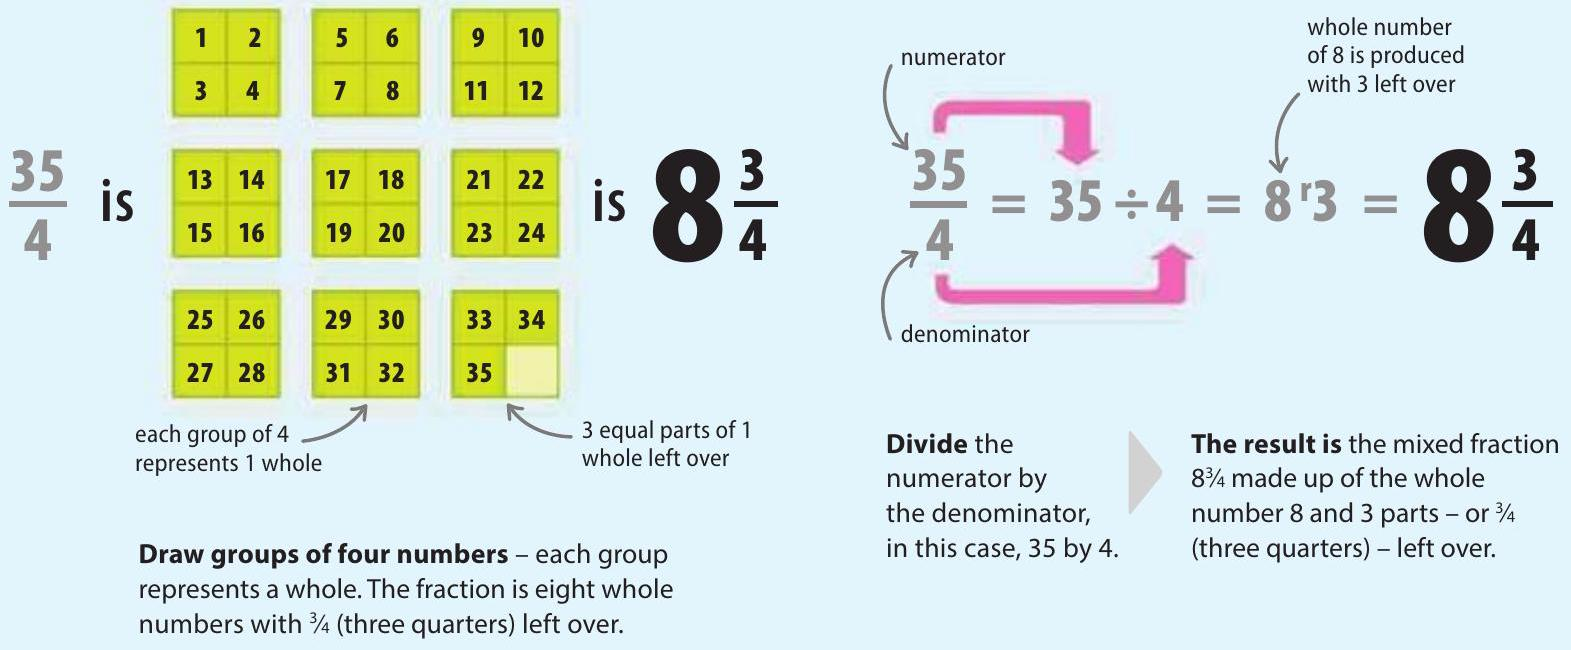
\includegraphics[max width=\textwidth, center]{2025_07_08_04014fa2c17a4b6cdcc6g-052}

\section*{Turning mixed fractions into top-heavy fractions}
A mixed fraction can be changed into a top-heavy fraction by multiplying the whole number by the denominator and adding the result to the numerator.\\
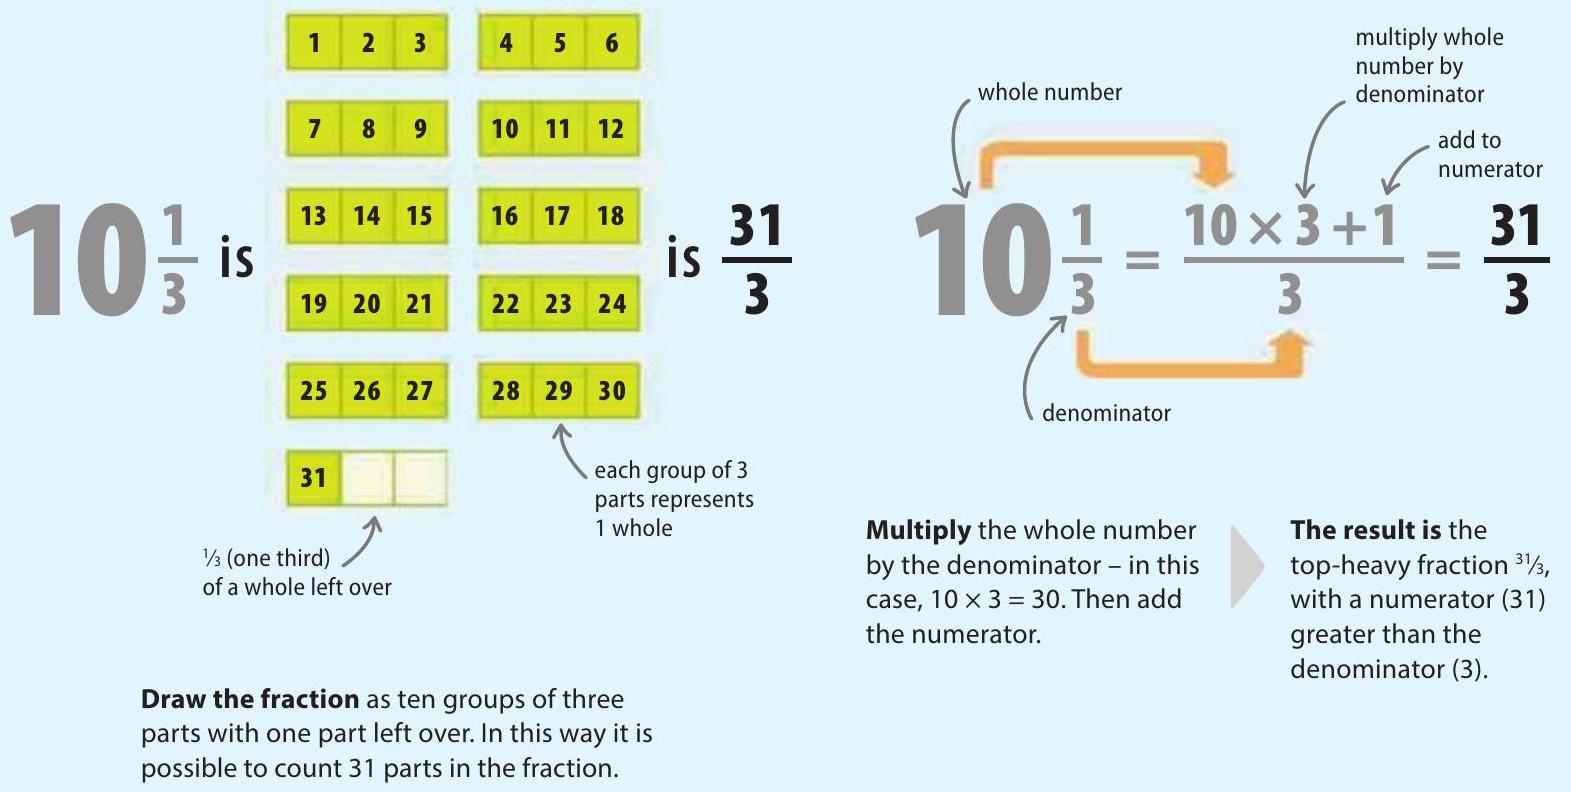
\includegraphics[max width=\textwidth, center]{2025_07_08_04014fa2c17a4b6cdcc6g-052(1)}

\section*{Equivalent fractions}
The same fraction can be written in different ways. These are known as equivalent (meaning "equal") fractions, even though they look different.\\
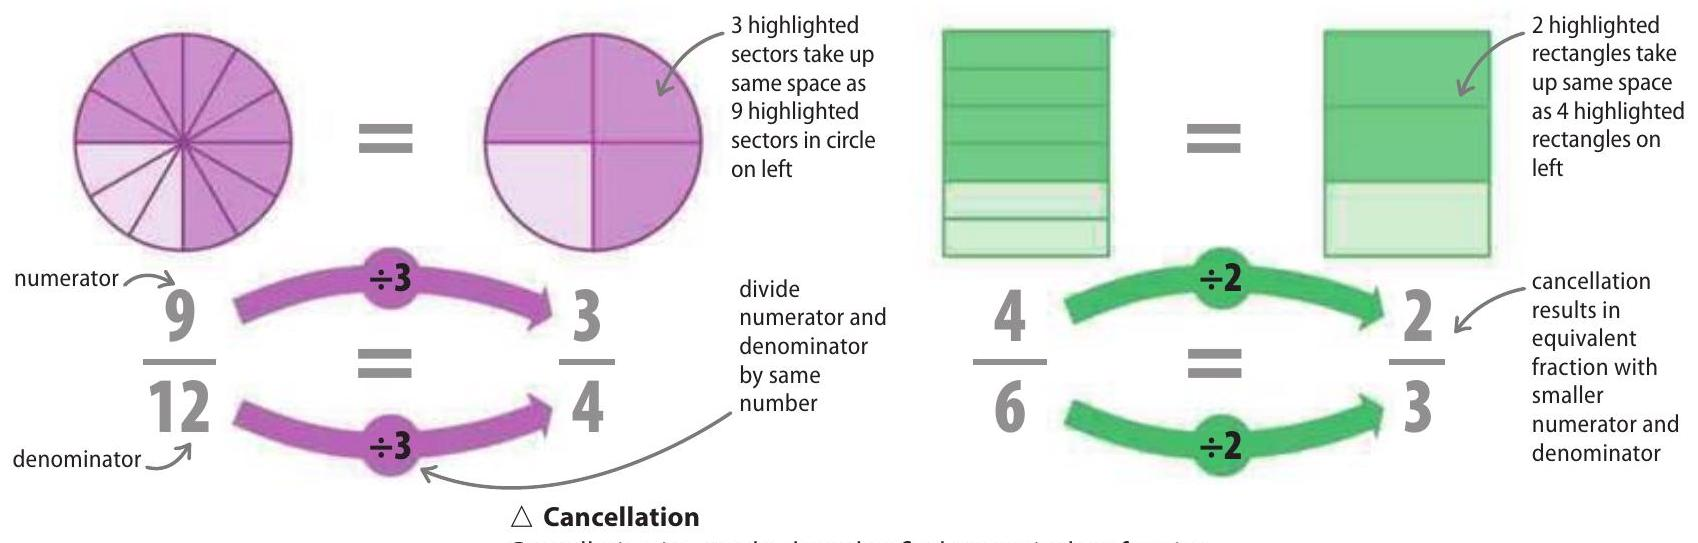
\includegraphics[max width=\textwidth, center]{2025_07_08_04014fa2c17a4b6cdcc6g-053}

Cancellation is a method used to find an equivalent fraction that is simpler than the original. To cancel a fraction divide the numerator and denominator by the same number.\\
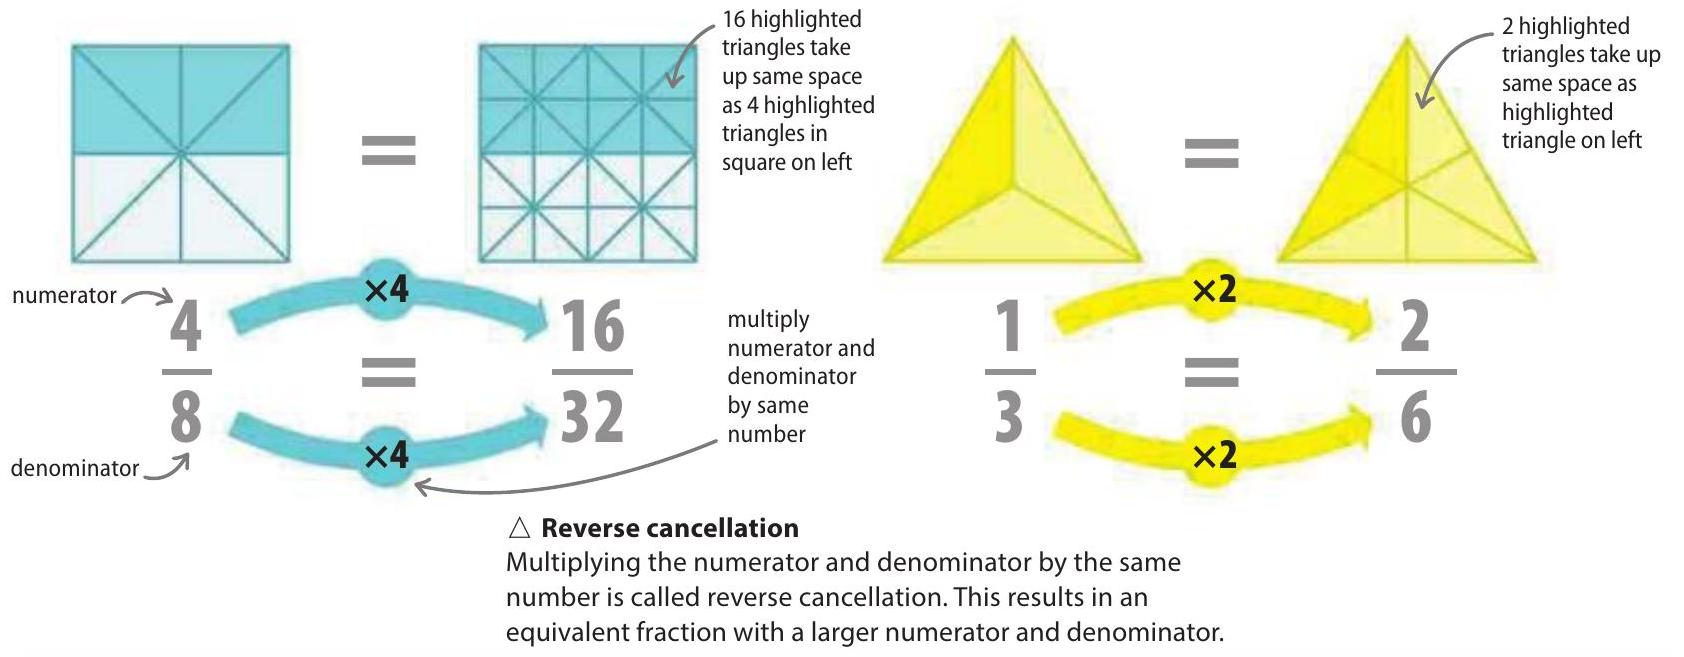
\includegraphics[max width=\textwidth, center]{2025_07_08_04014fa2c17a4b6cdcc6g-053(1)}

\begin{center}
\begin{tabular}{|l|l|l|l|l|l|l|l|l|l|}
\hline
\multicolumn{10}{|c|}{Table of equivalent fractions} \\
\hline
$1 / 1=$ & 2/2 & 3/3 & 4/4 & 5/5 & 6/6 & 7/7 & 8/8 & 9/9 & 10/10 \\
\hline
$1 / 2=$ & 2/4 & 3/6 & 4/8 & 5/10 & 6/12 & 7/14 & 8/16 & 9/18 & 10/20 \\
\hline
$1 / 3=$ & 2/6 & 3/9 & 4/12 & 5/15 & 6/18 & 7/21 & 8/24 & 9/27 & 10/30 \\
\hline
$1 / 4=$ & 2/8 & 3/12 & 4/16 & 5/20 & 6/24 & 7/28 & 8/32 & 9/36 & 10/40 \\
\hline
$1 / 5=$ & 2/10 & 3/15 & 4/20 & 5/25 & 6/30 & 7/35 & 8/40 & 9/45 & 10/50 \\
\hline
$1 / 6=$ & 2/12 & 3/18 & 4/24 & 5/30 & 6/36 & 7/42 & 8/48 & 9/54 & 10/60 \\
\hline
$1 / 7=$ & 2/14 & 3/21 & 4/28 & 5/35 & 6/42 & 7/49 & 8/56 & 9/63 & 10/70 \\
\hline
$1 / 8=$ & 2/16 & 3/24 & 4/32 & 5/40 & 6/48 & 7/56 & 8/64 & 9/72 & 10/80 \\
\hline
\end{tabular}
\end{center}

\section*{Finding a common denominator}
When finding the relative sizes of two or more fractions, finding a common denominator makes it much easier. A common denominator is a number that can be divided by the denominators of all of the fractions. Once this has been found, comparing fractions is just a matter of comparing their numerators.

\section*{$\triangleright$ Comparing fractions}
To work out the relative sizes of fractions, it is necessary to convert them so that they all have the same denominator. To do so, first look at the denominators of all the fractions being compared.

\section*{- Make a list}
List the multiples - all the whole number products of each denominator - for all of the denominators. Pick a sensible stopping point for the list, such as 100.\\
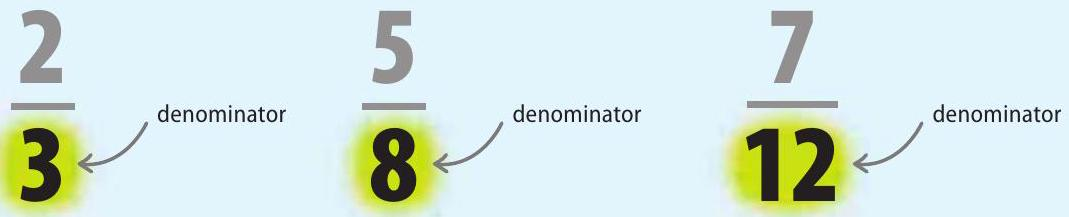
\includegraphics[max width=\textwidth, center]{2025_07_08_04014fa2c17a4b6cdcc6g-054(1)}

\begin{center}
\begin{tabular}{lll}
$\mathbf{3}, \mathbf{6}, \mathbf{9}, \mathbf{1 2}$, & $\mathbf{8}, \mathbf{1 6}, \mathbf{2 4}, \mathbf{3 2}$, & $\mathbf{1 2}, \mathbf{2 4}, \mathbf{3 6}$, \\
$\mathbf{1 5}, \mathbf{1 8}, \mathbf{2 1}$, & $\mathbf{4 0}, \mathbf{4 8}, \mathbf{5 6}$, & $\mathbf{4 8}, \mathbf{6 0}, \mathbf{7 2}$, \\
$\mathbf{2 4}, \mathbf{2 7}, \mathbf{3 0}, \ldots$ & $\mathbf{6 4}, \mathbf{7 2}, \ldots$ & $\mathbf{8 4}, \mathbf{9 6}, \ldots$ \\
\end{tabular}
\end{center}

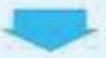
\includegraphics[max width=\textwidth, center]{2025_07_08_04014fa2c17a4b6cdcc6g-054}\\
$\triangleright$ Find the lowest common denominator\\
List only the multiples that are common to all three sets. These numbers are called common denominators. Identify the lowest one.\\
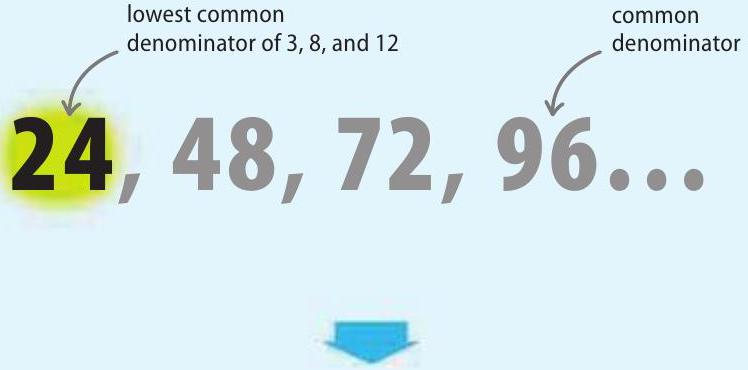
\includegraphics[max width=\textwidth, center]{2025_07_08_04014fa2c17a4b6cdcc6g-054(2)}

\begin{itemize}
  \item Convert the fractions
\end{itemize}

Find out how many times the original denominator goes into the common denominator. Multiply the numerator by the same number. It is now possible to compare the fractions.\\
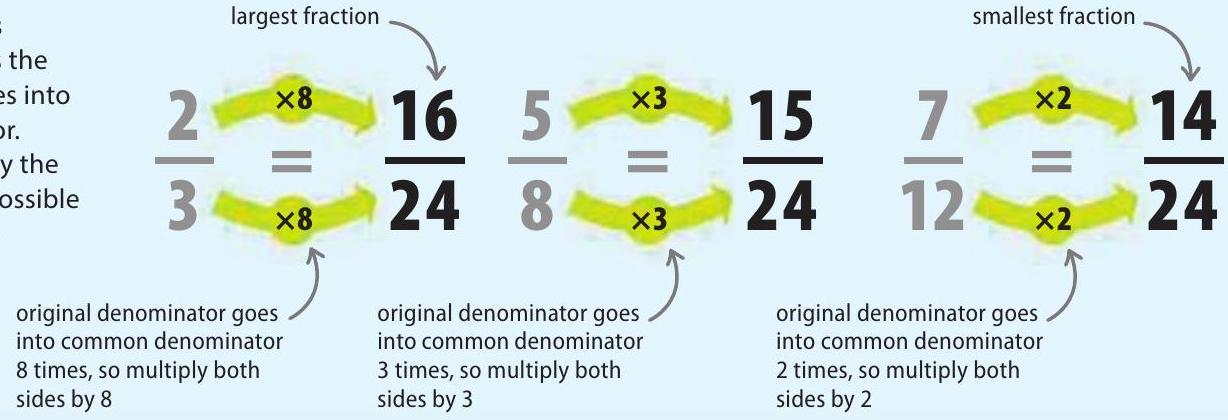
\includegraphics[max width=\textwidth, center]{2025_07_08_04014fa2c17a4b6cdcc6g-054(3)}

\section*{ADDING AND SUBTRACTING FRACTIONS}
Just like whole numbers, it is possible to add and subtract fractions. How it is done depends on whether the denominators are the same or different.

\section*{Adding and subtracting fractions with the same denominator}
To add or subtract fractions that have the same denominator, simply add or subtract their numerators to get the answer. The denominators stay the same.\\
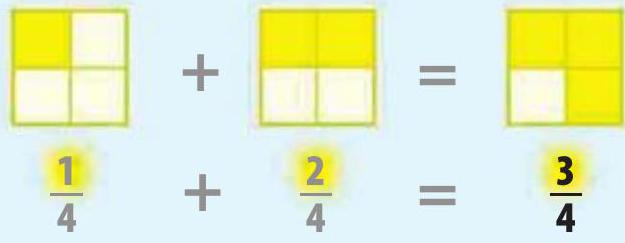
\includegraphics[max width=\textwidth, center]{2025_07_08_04014fa2c17a4b6cdcc6g-055(1)}

To add fractions, add together only the numerators. The denominator in the result remains unchanged.\\
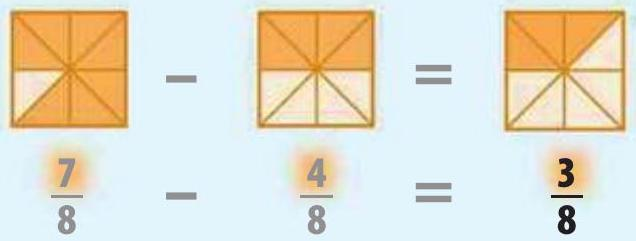
\includegraphics[max width=\textwidth, center]{2025_07_08_04014fa2c17a4b6cdcc6g-055(3)}

To subtract fractions, subtract the smaller numerator from the larger. The denominator in the result stays the same.

\section*{Adding fractions with different denominators}
To add fractions that have different denominators, it is necessary to change one or both of the fractions so they have the same denominator. This involves finding a common denominator (see opposite).\\
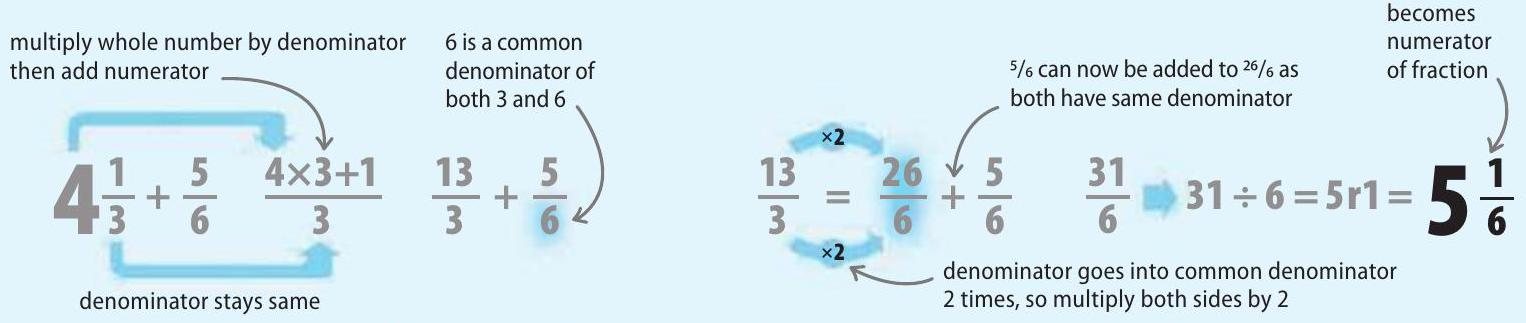
\includegraphics[max width=\textwidth, center]{2025_07_08_04014fa2c17a4b6cdcc6g-055(2)}

First, turn any mixed fractions that are being added into top-heavy fractions.

It is not possible to add fractions with different denominators, so find a common denominator.

Convert the fractions\\
into fractions with common denominators by multiplying.

In order to turn the resulting top-heavy fraction back into a mixed fraction, divide the numerator by the denominator.

\section*{Subtracting fractions with different denominators}
To subtract fractions with different denominators, a common denominator must be found.\\
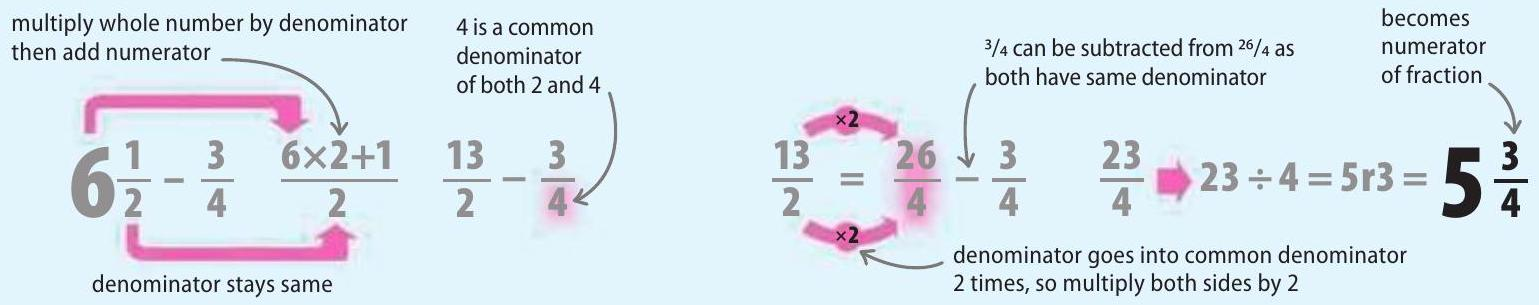
\includegraphics[max width=\textwidth, center]{2025_07_08_04014fa2c17a4b6cdcc6g-055}

First, turn any mixed fractions in the equation into top-heavy fractions by multiplying.

The two fractions have different denominators, so a common denominator is needed.

Convert the fractions into fractions with common denominators by multiplying.

If necessary, divide the numerator by the denominator to turn the top-heavy fraction back into a mixed fraction.

\section*{MULTIPLYING FRACTIONS}
Fractions can be multiplied by other fractions. To multiply fractions by mixed fractions or whole numbers, they first need to be converted into top-heavy fractions.\\
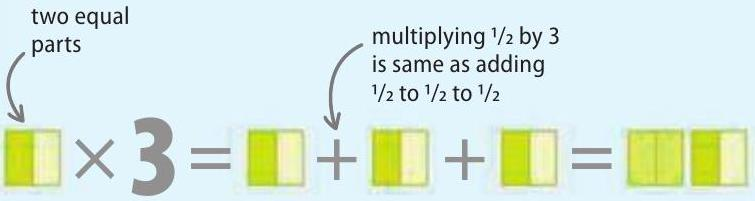
\includegraphics[max width=\textwidth, center]{2025_07_08_04014fa2c17a4b6cdcc6g-056(4)}

$$
\frac{1}{2} \times \mathbf{3}=\frac{1}{2}+\frac{1}{2}+\frac{1}{2}=\mathbf{1} \frac{1}{2}
$$

Imagine multiplying a fraction by a whole number as adding the fraction to itself that many times. Alternatively, imagine multiplying a whole number by a fraction as taking that portion of the whole number, here $1 / 2$ of 3 .\\
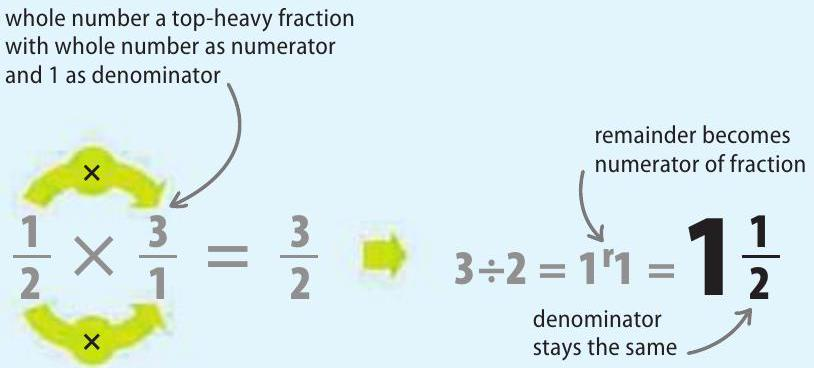
\includegraphics[max width=\textwidth, center]{2025_07_08_04014fa2c17a4b6cdcc6g-056(5)}

Convert the whole number to a fraction. Next, multiply both numerators together and then both denominators.

\section*{Multiplying two proper fractions}
Proper fractions can be multiplied by each other. It is useful to imagine the multiplication sign means "of" - the sum below can be expressed as "what is $1 / 2$ of $3 / 4$ ?" and "what is $3 / 4$ of $1 / 2$ ?".\\
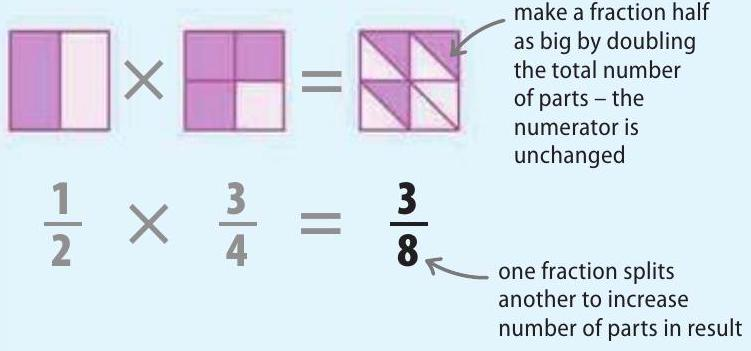
\includegraphics[max width=\textwidth, center]{2025_07_08_04014fa2c17a4b6cdcc6g-056}

Visually, the result of multiplying two proper fractions is that the space taken up by both together is reduced.\\
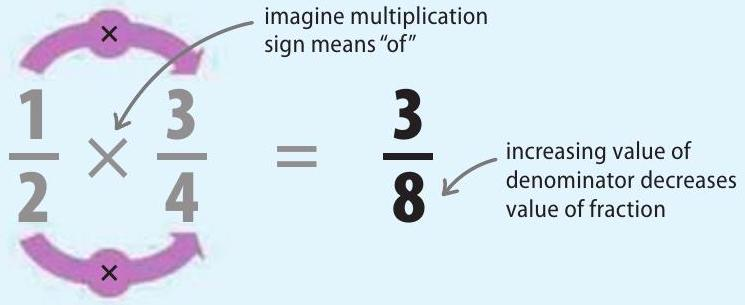
\includegraphics[max width=\textwidth, center]{2025_07_08_04014fa2c17a4b6cdcc6g-056(1)}

Multiply the numerators and the denominators. The resulting fraction answers both questions: "what is $1 / 2$ of $3 / 4$ ?" and "what is $3 / 4$ of $1 / 2$ ?".

\section*{Multiplying mixed fractions}
To multiply a proper fraction by a mixed fraction, it is necessary to first convert the mixed fraction into a top-heavy fraction.\\
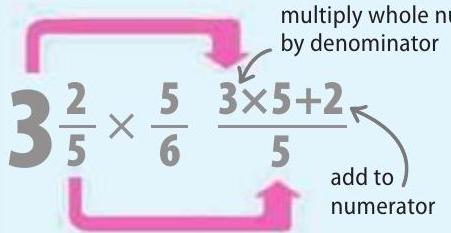
\includegraphics[max width=\textwidth, center]{2025_07_08_04014fa2c17a4b6cdcc6g-056(3)}

First, turn the mixed fraction into a top-heavy fraction.\\
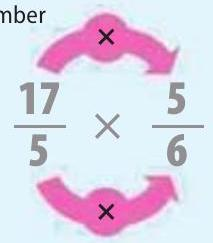
\includegraphics[max width=\textwidth, center]{2025_07_08_04014fa2c17a4b6cdcc6g-056(2)}

Next, multiply the numerators and denominators of both fractions to get a new fraction.\\
to show in its lowest form divide both numbers by 5 to get $5 / 6$

\section*{DIVIDING FRACTIONS}
Fractions can be divided by whole numbers. To do so turn the whole number into a fraction, turn the fraction upside down, then multiply it by the first fraction.\\
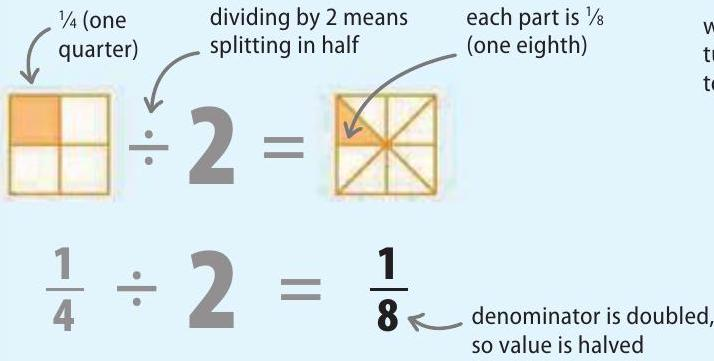
\includegraphics[max width=\textwidth, center]{2025_07_08_04014fa2c17a4b6cdcc6g-057}

Picture dividing a fraction by a whole number as splitting it into that many parts. In this example, $1 / 4$ is split in half, resulting in twice as many equal parts.\\
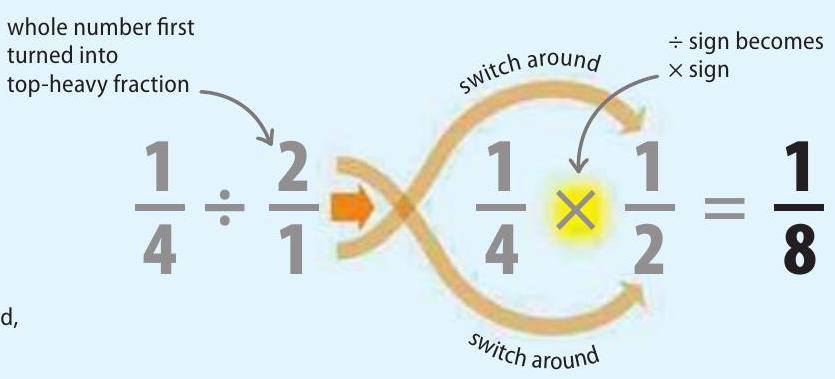
\includegraphics[max width=\textwidth, center]{2025_07_08_04014fa2c17a4b6cdcc6g-057(2)}

To divide a fraction by a whole number, convert the whole number into a fraction, turn the fraction upside down, and multiply both the numerators and the denominators.

\section*{Dividing two proper fractions}
Proper fractions can be divided by other proper fractions by using an inverse operation. Multiplication and division are inverse operations as they are the opposite of each other.\\
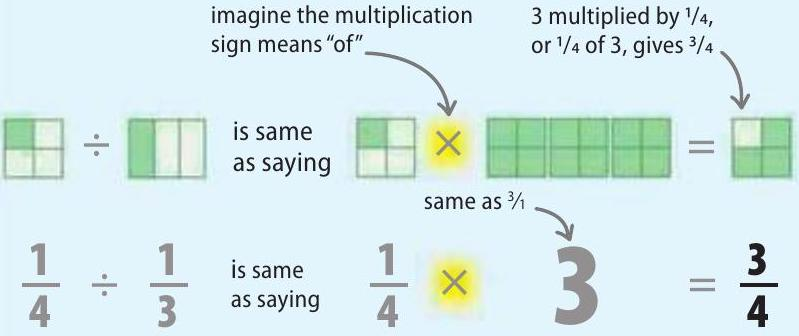
\includegraphics[max width=\textwidth, center]{2025_07_08_04014fa2c17a4b6cdcc6g-057(3)}

Dividing one fraction by another is the same as turning the second fraction upside down and then multiplying the two.\\
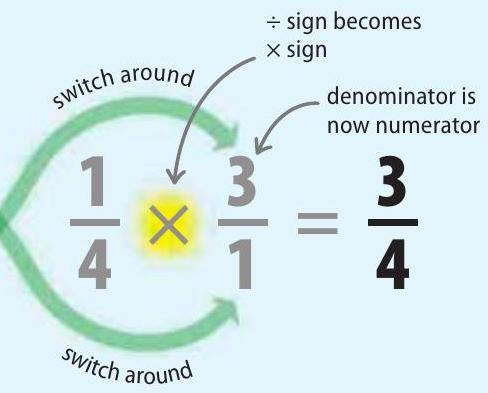
\includegraphics[max width=\textwidth, center]{2025_07_08_04014fa2c17a4b6cdcc6g-057(1)}

To divide two fractions use the inverse operation turn the last fraction upside down, then multiply both the numerators and the denominators.

\section*{Dividing mixed fractions}
To divide mixed fractions, first convert them into top-heavy fractions, then turn the second fraction upside down and multiply it by the first.\\
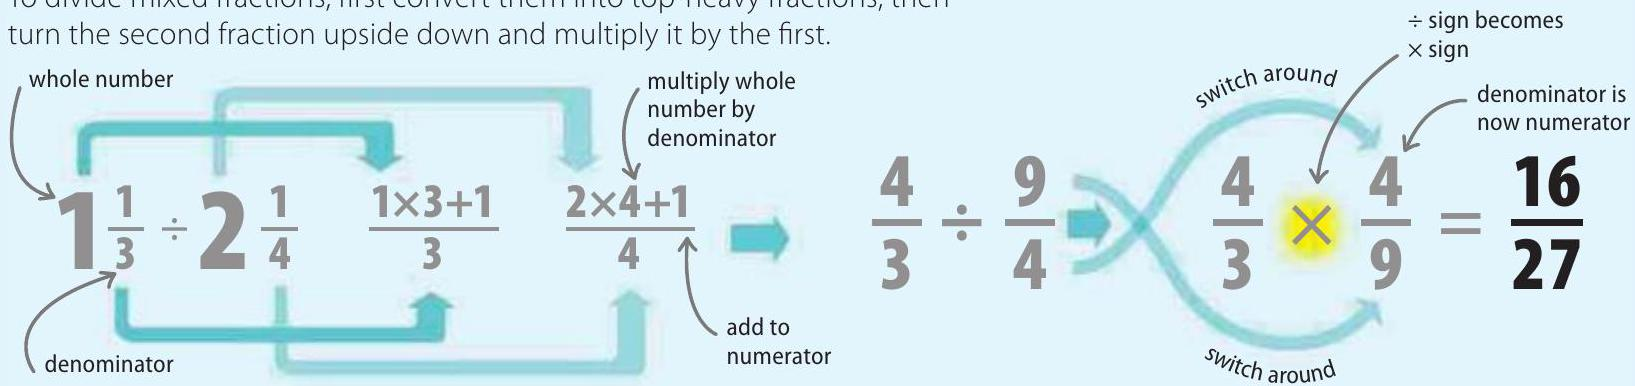
\includegraphics[max width=\textwidth, center]{2025_07_08_04014fa2c17a4b6cdcc6g-057(4)}

First, turn both the mixed fractions into top-heavy fractions by multiplying the whole number by the

Divide the two fractions by turning the second denominator and adding the numerator. fraction upside down, then multiplying both the numerators and the denominators.

\section*{- Ratio and proportion}
RATIO COMPARES THE SIZE OF QUANTITIES. PROPORTION COMPARES THE RELATIONSHIP BETWEEN TWO SETS OF QUANTITIES.

\begin{center}
\begin{tabular}{|l|}
\hline
SEE ALSO \\
\hline
< 18-21 \\
\hline
<22-25 Division \\
\hline
<48-55 \\
\hline
\end{tabular}
\end{center}

Ratios show how much bigger one thing is than another. Two things are in proportion when a change in one causes a related change in the other.

\section*{Writing ratios}
Ratios are written as two or more numbers with a colon between each. For example, a fruit bowl in which the ratio of apples to pears is $2: 1$ means that there are 2 apples for every 1 pear in the bowl.\\
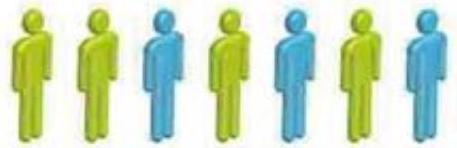
\includegraphics[max width=\textwidth, center]{2025_07_08_04014fa2c17a4b6cdcc6g-058}

Supporters\\
This group represents fans of two football clubs, the "greens" and the "blues".

\section*{- Forming a ratio}
To compare the numbers of people who support the two different clubs, write them as a ratio. This makes it clear that for every 4 green fans there are 3 blue fans.\\
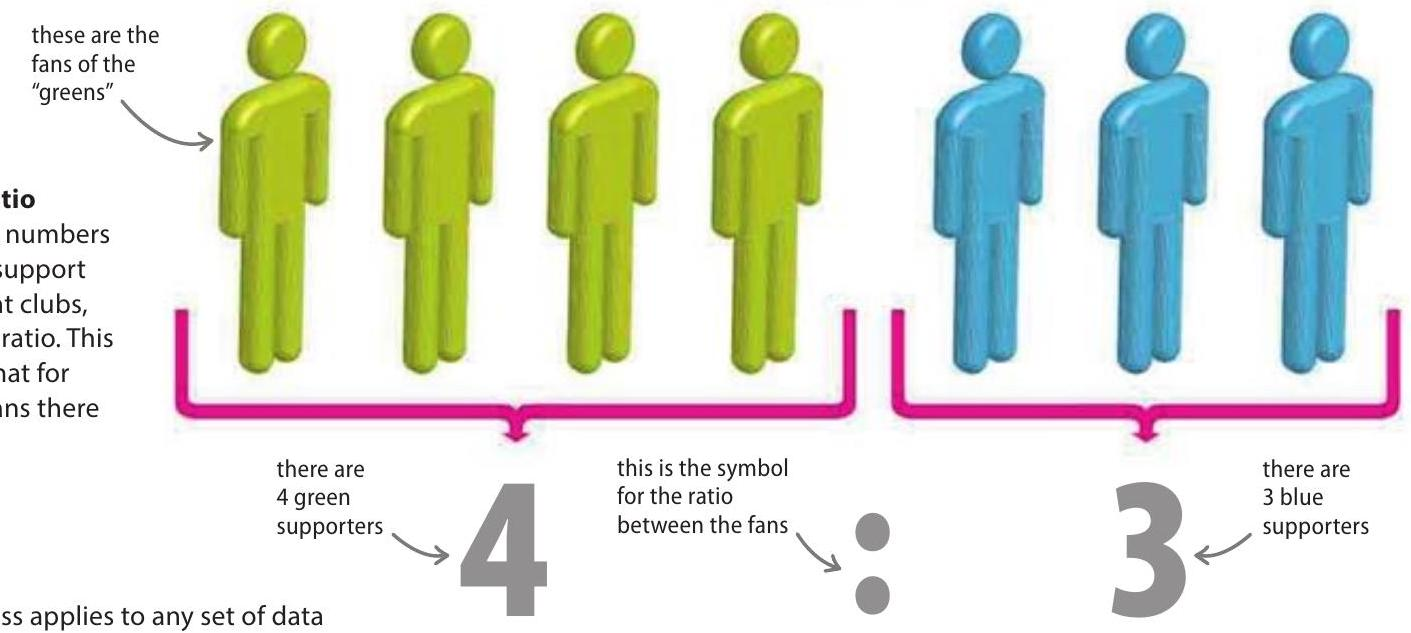
\includegraphics[max width=\textwidth]{2025_07_08_04014fa2c17a4b6cdcc6g-058(3)} that needs comparing. Here are more groups of fans, and the ratios they represent.\\
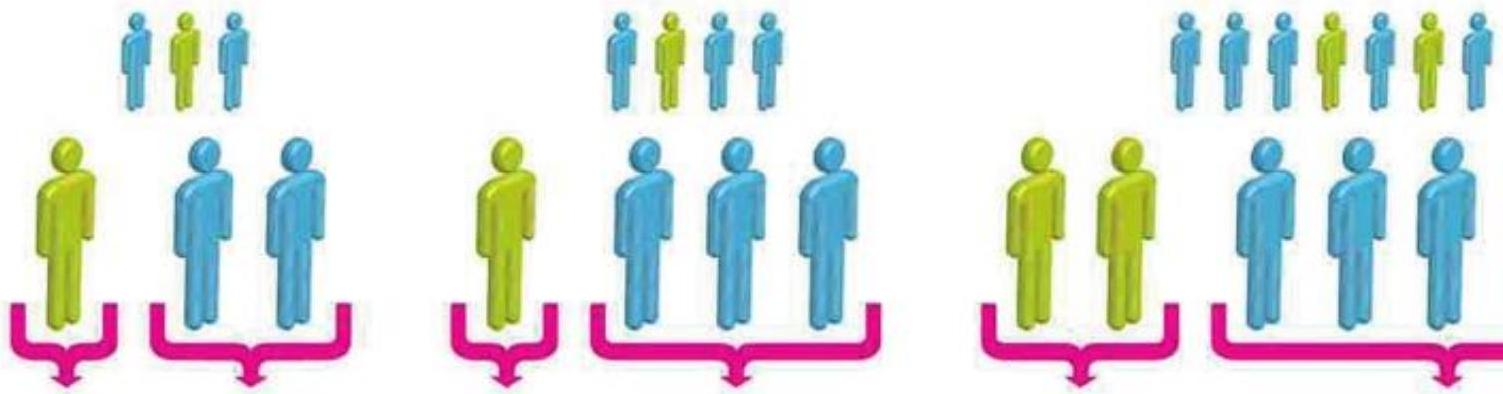
\includegraphics[max width=\textwidth, center]{2025_07_08_04014fa2c17a4b6cdcc6g-058(4)}

\section*{1: 2}
$\triangle 1: 2$\\
One fan of the greens and 2 fans of the blues can be compared as the ratio $1: 2$. This means that in this case there are twice as many fans of the blues as of the greens.\\
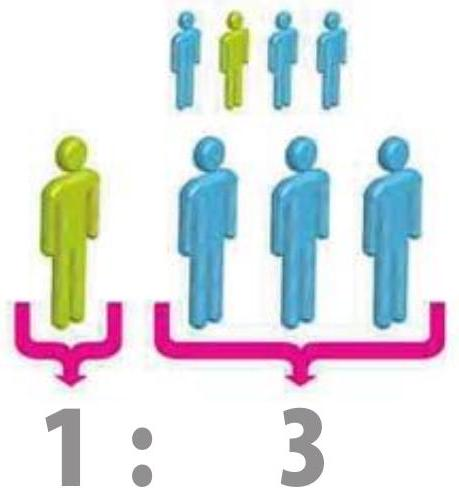
\includegraphics[max width=\textwidth, center]{2025_07_08_04014fa2c17a4b6cdcc6g-058(1)}\\
$\triangle 1: 3$\\
One fan of the greens and 3 fans of the blues can be shown as the ratio $1: 3$, which means that, in this case, there are three times more blue fans than green fans.\\
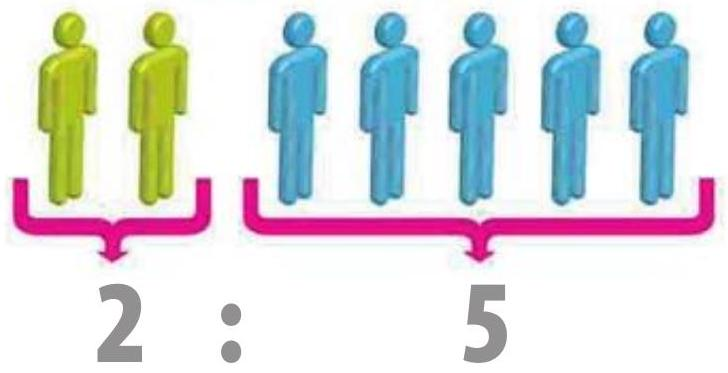
\includegraphics[max width=\textwidth, center]{2025_07_08_04014fa2c17a4b6cdcc6g-058(2)}\\
$\triangle 2: 5$\\
Two fans of the greens and 5 fans of the blues can be compared as the ratio $2: 5$. There are more than twice as many fans of the blues as of the greens.

\section*{Finding a ratio}
Large numbers can also be written as ratios. For example, to find the ratio between 1 hour and 20 minutes, convert them into the same unit, then cancel these numbers by finding the highest number that divides into both.

\section*{minutes are the新 smaller unit}
\begin{center}
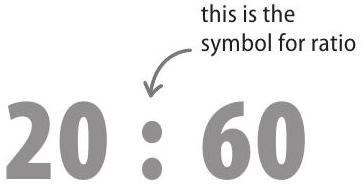
\includegraphics[max width=\textwidth]{2025_07_08_04014fa2c17a4b6cdcc6g-059(2)}
\end{center}

Write as a ratio by inserting a colon between the two quantities.\\
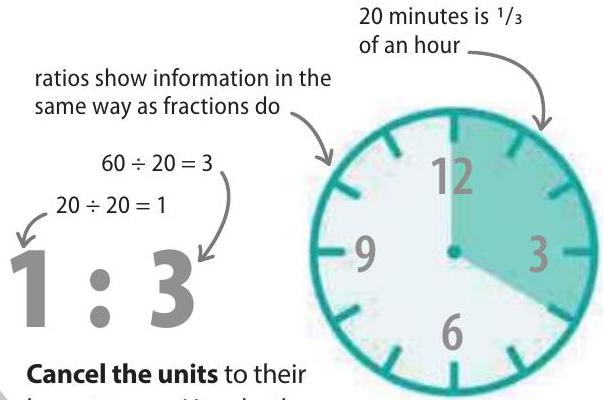
\includegraphics[max width=\textwidth]{2025_07_08_04014fa2c17a4b6cdcc6g-059} lowest terms. Here both sides divide exactly by 20 to give the ratio $1: 3$.

\section*{Working with ratios}
Ratios can represent real values. In a scale, the small number of the ratio is the value on the scale model, and the larger is the real value it represents.\\
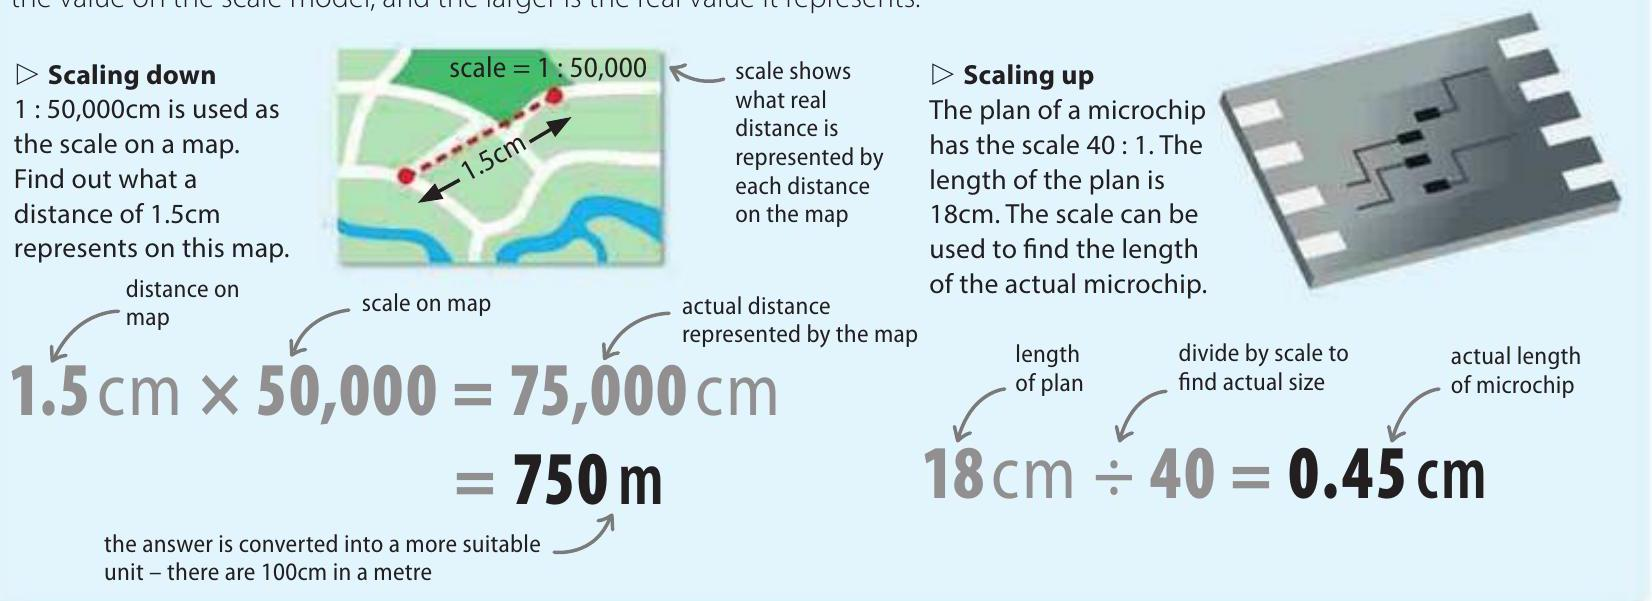
\includegraphics[max width=\textwidth, center]{2025_07_08_04014fa2c17a4b6cdcc6g-059(4)}

\section*{Comparing ratios}
Converting ratios into fractions allows their size to be compared. To compare the ratios $4: 5$ and $1: 2$, write them as fractions with the same denominator.\\
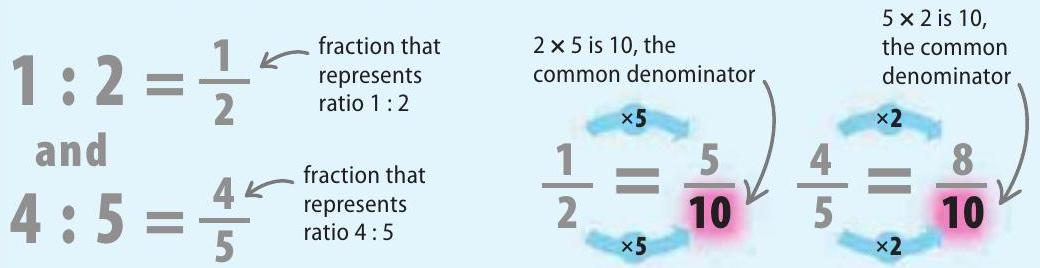
\includegraphics[max width=\textwidth, center]{2025_07_08_04014fa2c17a4b6cdcc6g-059(3)}

First write each ratio as a fraction, placing the smaller quantity in each above the larger quantity.

Convert the fractions so that they both have the same denominator, by multiplying the first fraction by 5 and the second by 2 .\\
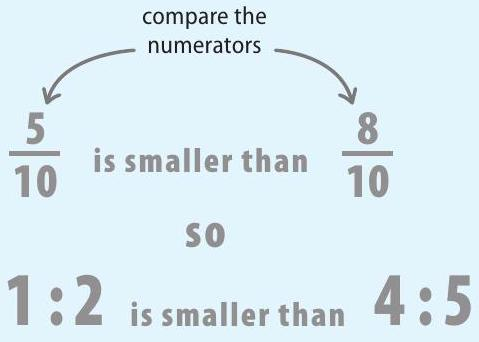
\includegraphics[max width=\textwidth, center]{2025_07_08_04014fa2c17a4b6cdcc6g-059(1)}

As the fractions now share a denominator, their sizes can be compared, making it clear which ratio is bigger.

\section*{PROPORTION}
Two quantities are in proportion when a change in one causes a change in the other.\\
Two examples of this are direct and indirect (also called inverse) proportion.

\section*{Direct proportion}
Two quantities are in direct proportion if the ratio between them is always the same. This means, for example, that if one quantity doubles then so does the other.\\
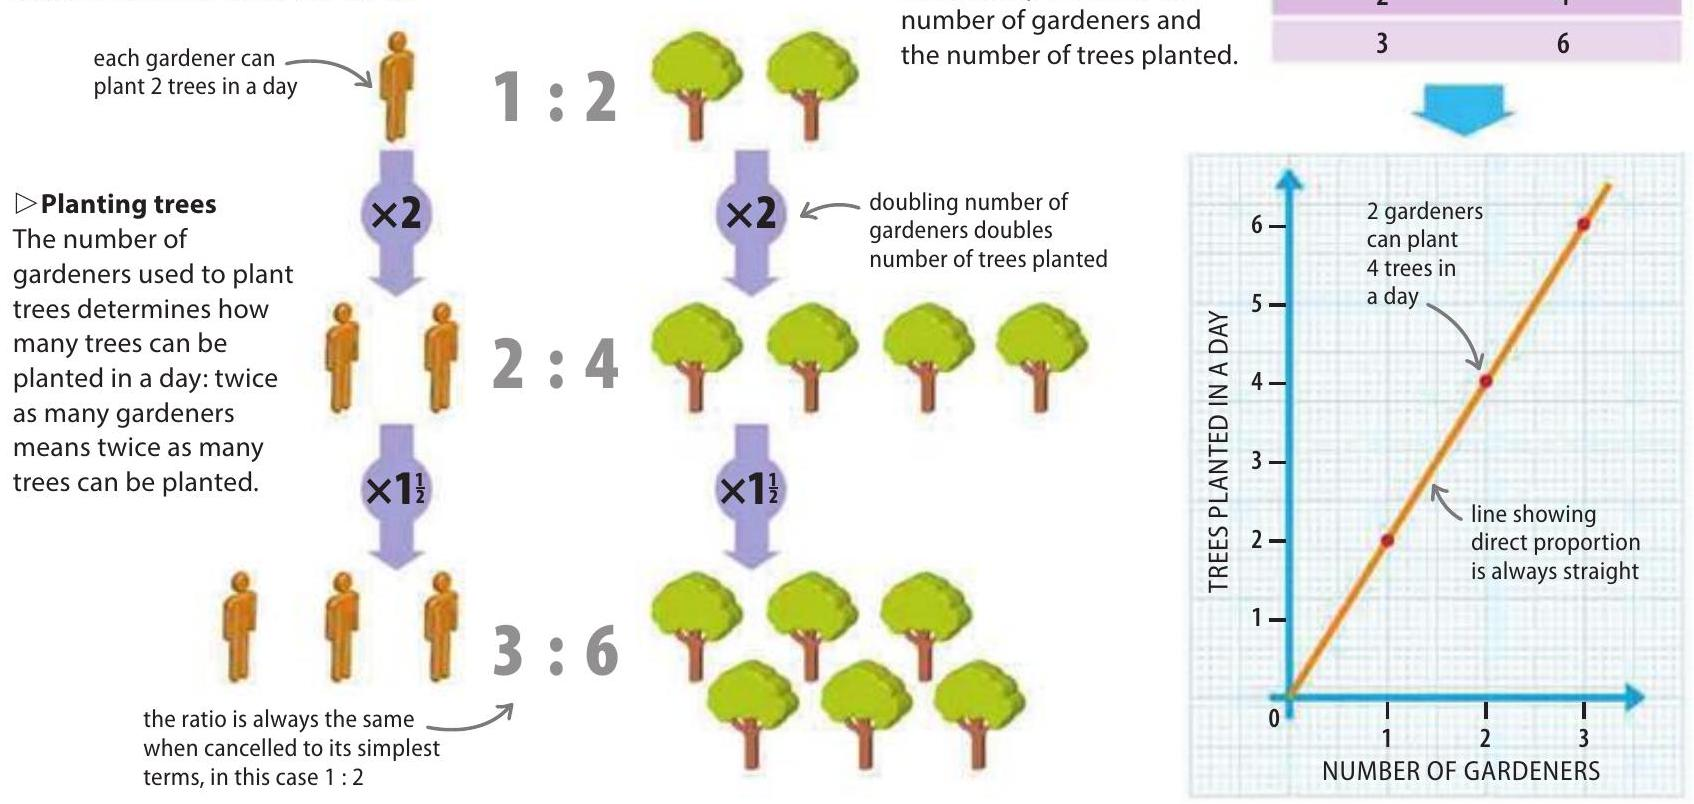
\includegraphics[max width=\textwidth, center]{2025_07_08_04014fa2c17a4b6cdcc6g-060(1)}

\section*{Indirect proportion}
Two quantities are in indirect proportion if their product (the answer when they are multiplied by each other) is always the same. So if one quantity doubles, the other quantity halves.

\section*{$\triangleright$ Delivering parcels}
The number of vans used to deliver parcels determines how many days it takes to deliver the parcels. Twice\\
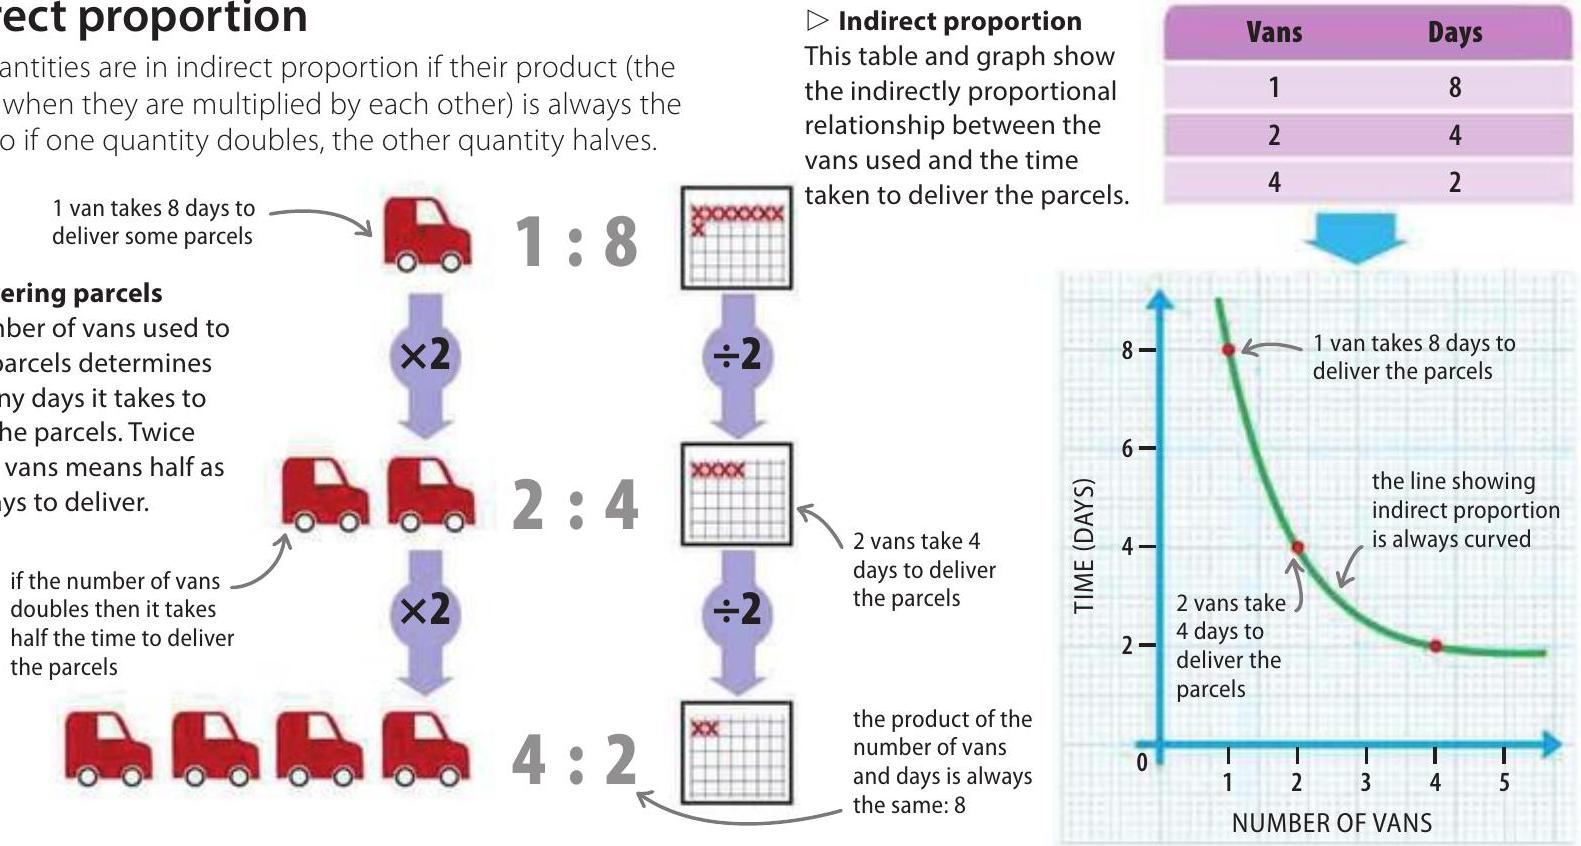
\includegraphics[max width=\textwidth, center]{2025_07_08_04014fa2c17a4b6cdcc6g-060}

\section*{Dividing in a given ratio}
A quantity can be divided into two, three, or more parts, according to a given ratio. This example shows how to divide 20 people into the ratios $2: 3$ and $6: 3: 1$.\\
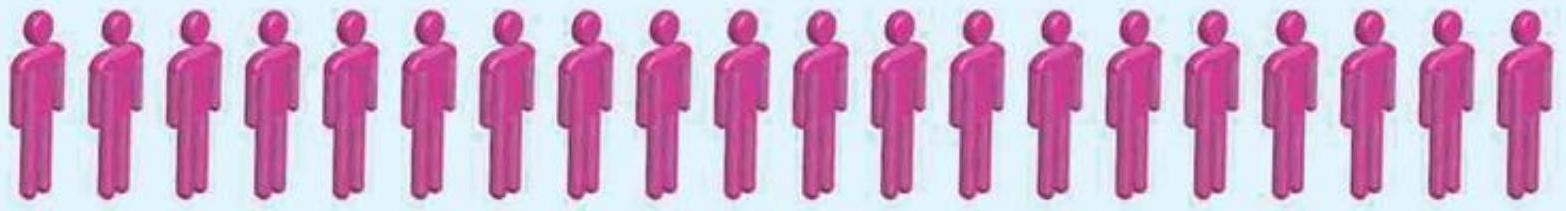
\includegraphics[max width=\textwidth, center]{2025_07_08_04014fa2c17a4b6cdcc6g-061(4)}

DIVIDING INTO A\\
TWO-PART RATIO\\
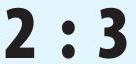
\includegraphics[max width=\textwidth, center]{2025_07_08_04014fa2c17a4b6cdcc6g-061}

\begin{displayquote}
total number of parts in the ratio $2+3=\mathbf{5}$\\
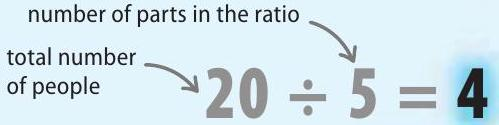
\includegraphics[max width=\textwidth, center]{2025_07_08_04014fa2c17a4b6cdcc6g-061(2)}\\
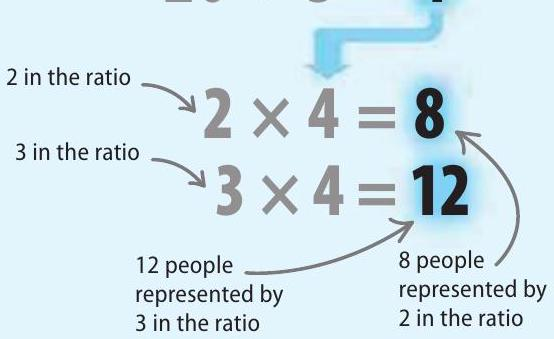
\includegraphics[max width=\textwidth, center]{2025_07_08_04014fa2c17a4b6cdcc6g-061(1)}
\end{displayquote}

These are the ratios to divide the people into.

Add the different parts of the ratio to find the total parts.

Divide the number of people by the parts of the ratio.

Multiply each part of the ratio by this quantity to find the size of the groups the ratios represent.

DIVIDING INTO A THREE-PART RATIO\\
6:3:1

$$
6+3+1=10
$$

\begin{center}
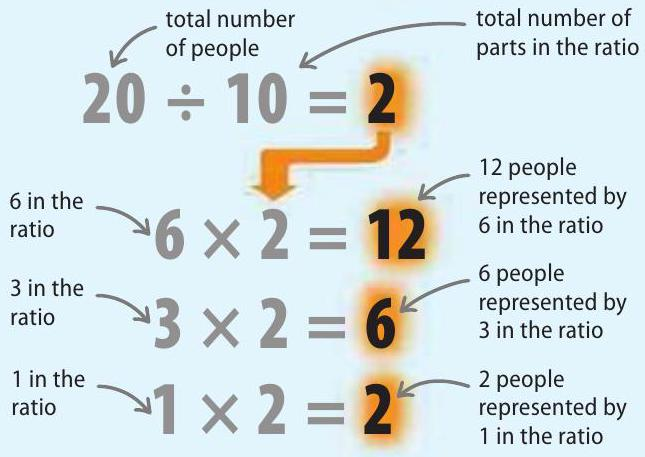
\includegraphics[max width=\textwidth]{2025_07_08_04014fa2c17a4b6cdcc6g-061(3)}
\end{center}

\section*{Proportional quantities}
Proportion can be used to solve problems involving unknown quantities. For example, if 3 bags contain 18 apples, how many apples do 5 bags contain?\\
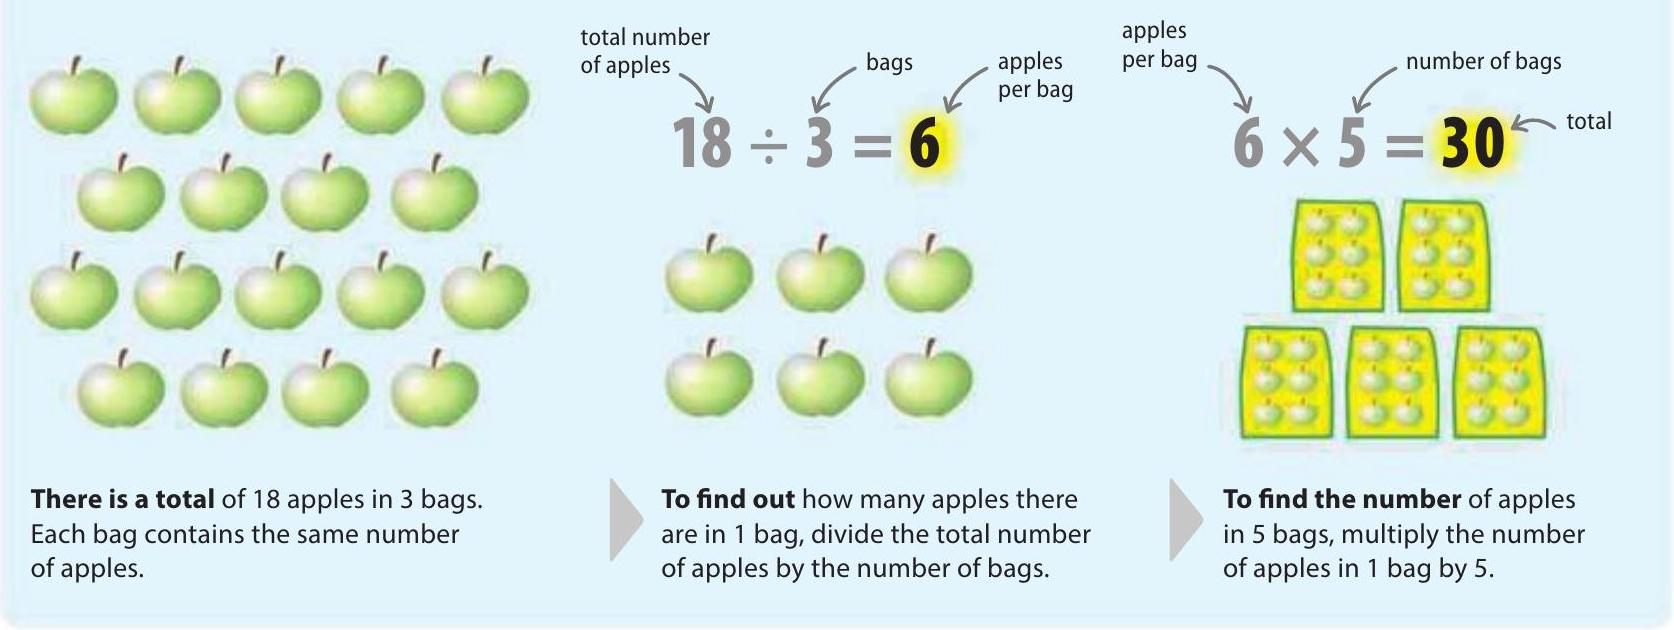
\includegraphics[max width=\textwidth, center]{2025_07_08_04014fa2c17a4b6cdcc6g-061(5)}

\section*{\% Percentages}
\section*{A PERCENTAGE SHOWS AN AMOUNT AS A PART OF 100.}
Any number can be written as a part of 100 or a percentage. Per cent means "per hundred", and it is a useful way of comparing two or more quantities.

\begin{center}
\begin{tabular}{|l|}
\hline
SEE ALSO \\
\hline
《 $\mathbf{4 4 - 4 5}$ Decimals \\
\hline
< 48-55 Fractions \\
\hline
\begin{tabular}{l}
Ratio and \\
proportion \\
\end{tabular} \\
\hline
Rounding off \\
\hline
\end{tabular}
\end{center}

The symbol " $\%$ " is used to indicate a percentage.

\section*{Parts of 100}
The simplest way to start looking at percentages is by dealing with a block of 100 units, as shown in the main image. These 100 units represent the total number of people in a school. This total can be divided into different groups according to the proportion of the total 100 they represent.

\section*{100\%}
This is simply another way of saying "everybody" or "everything". Here, all 100 figures 100\% - are blue.

\section*{50\%}
$\triangleright$ This group is equally divided between\\
50 blue and 50 purple figures. Each represents 50 out of 100 or $50 \%$ of the total. This is the same as half.

\section*{1\%}
$\triangleright$ In this group there is only 1 blue figure out of 100 , or $1 \%$.\\
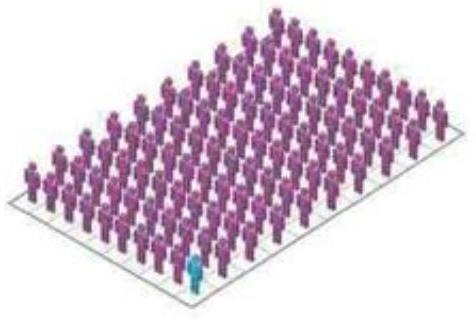
\includegraphics[max width=\textwidth, center]{2025_07_08_04014fa2c17a4b6cdcc6g-062}\\
$\triangle$ Adding up to 100\\
Percentages are an effective way to show the component parts of a total. For example, male teachers (blue) account for 5\% (5 out of 100) of the total.\\
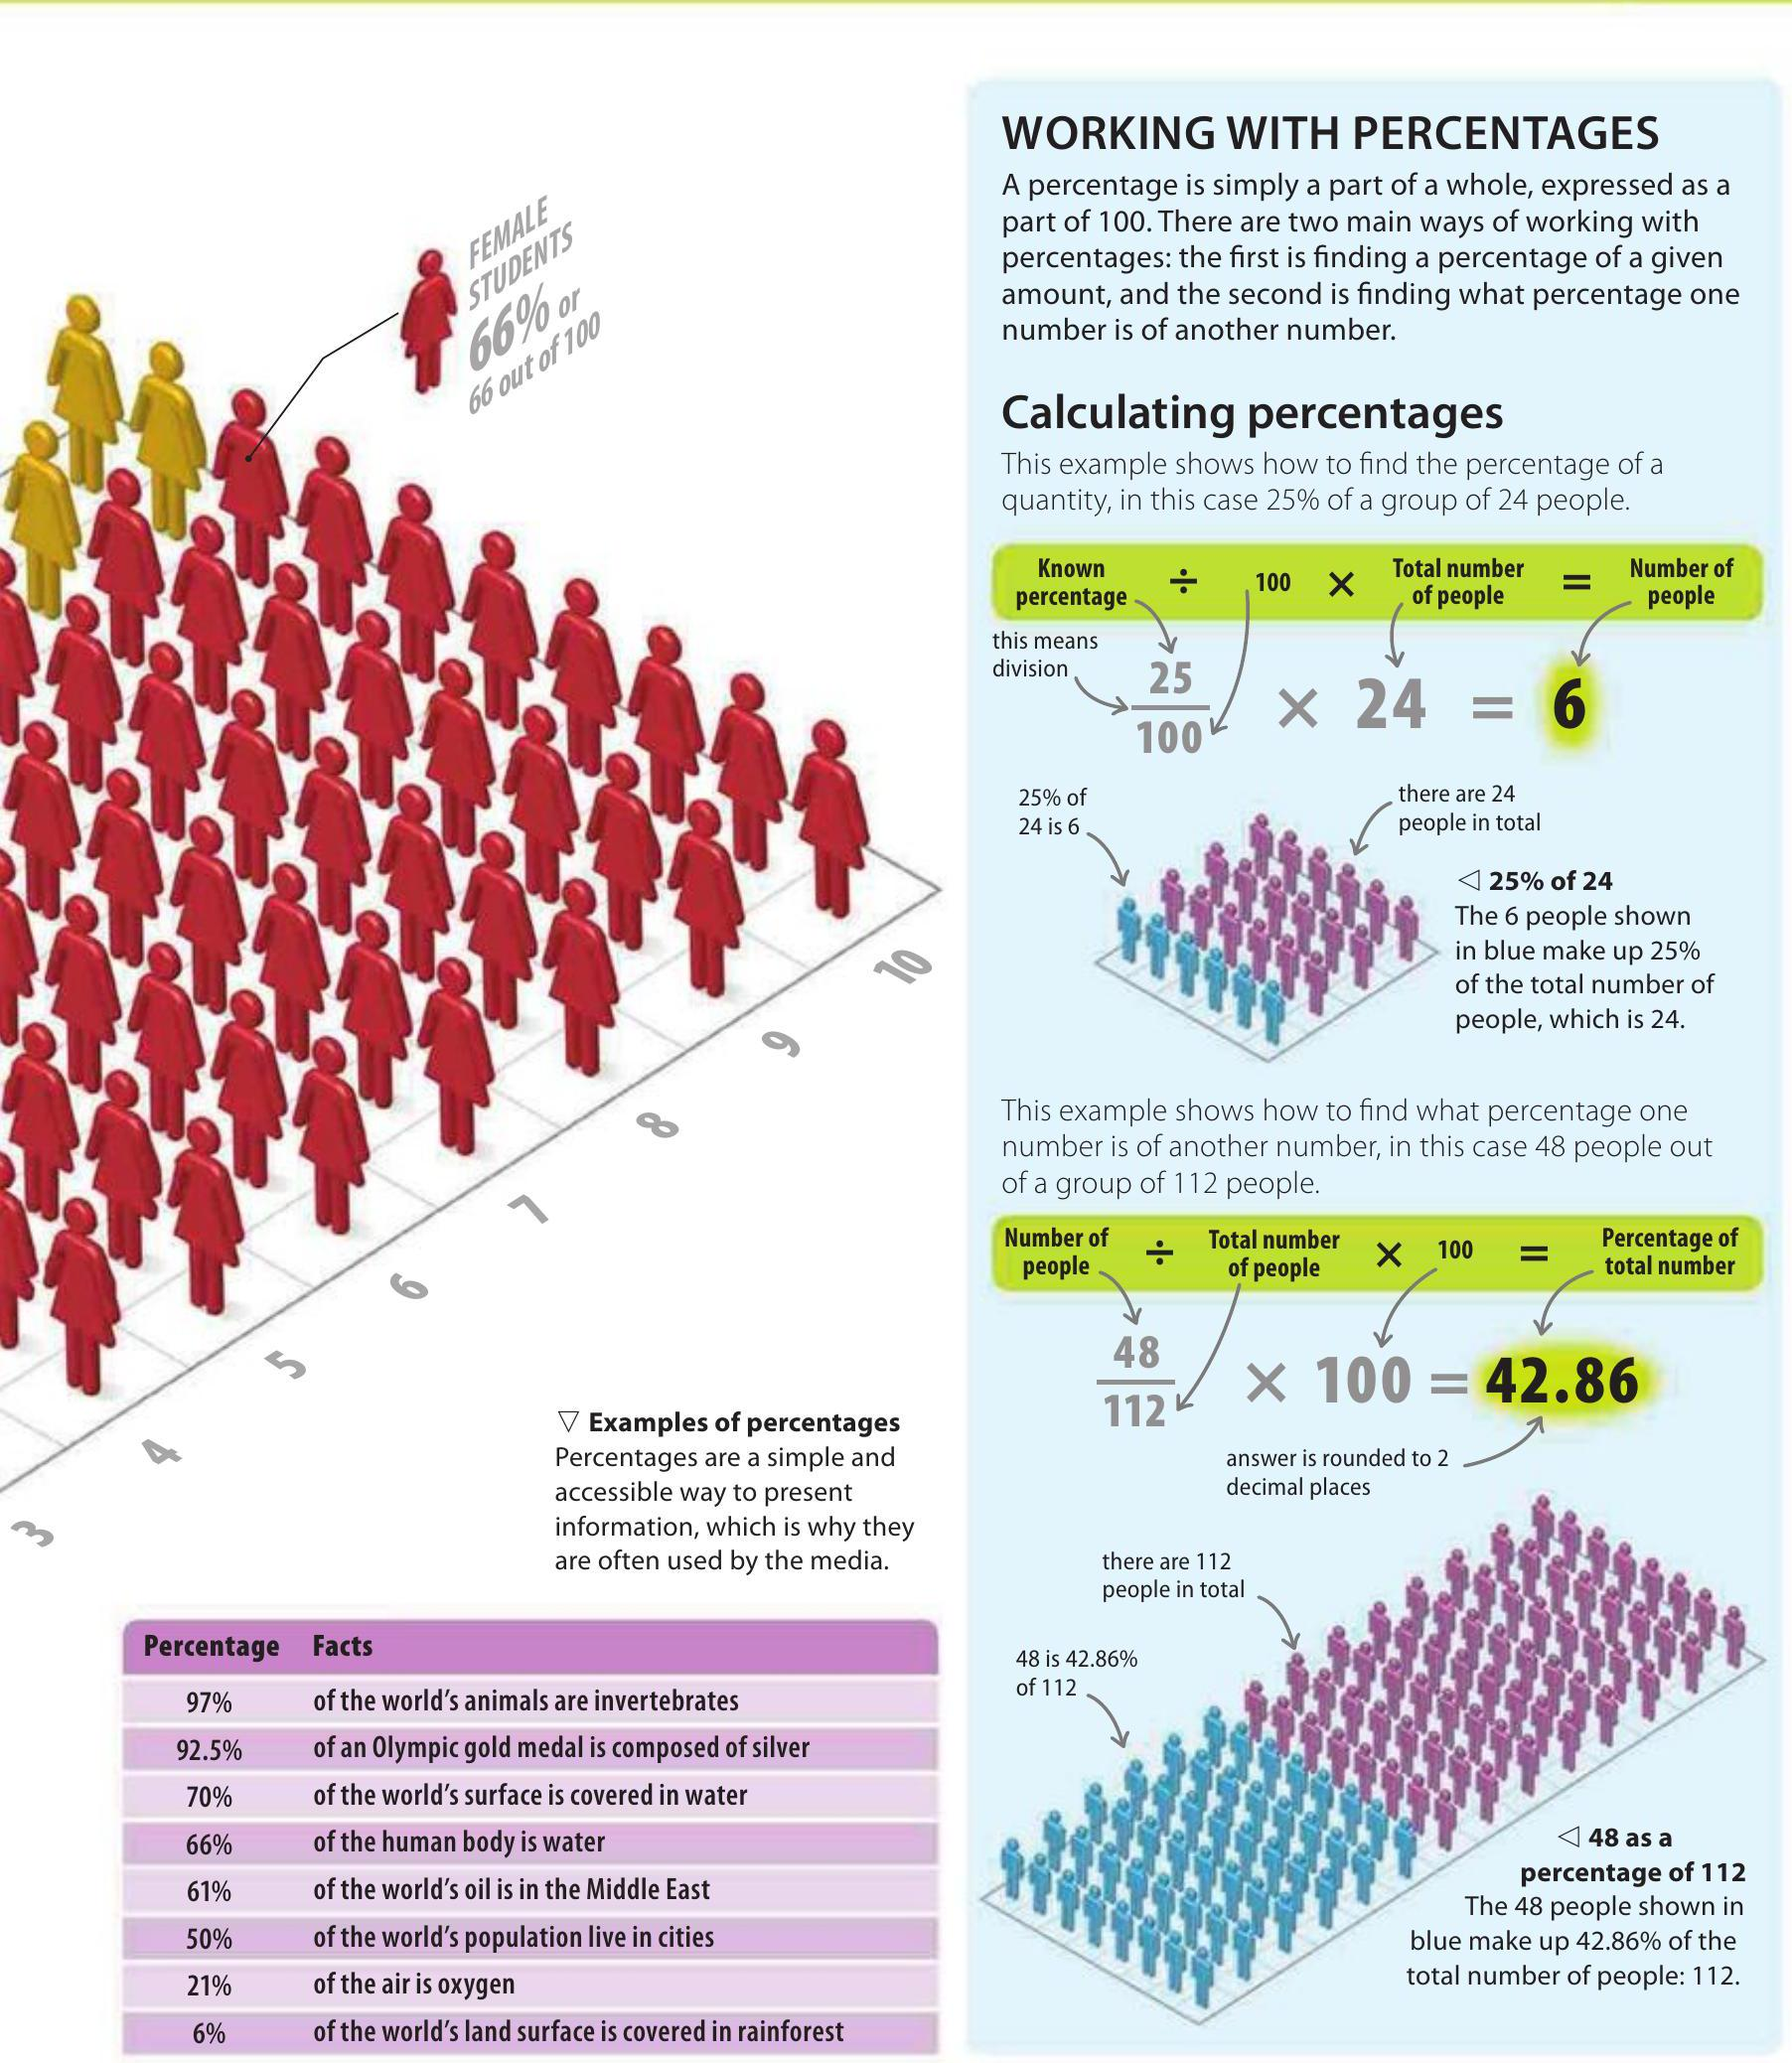
\includegraphics[max width=\textwidth, center]{2025_07_08_04014fa2c17a4b6cdcc6g-063}

\section*{PERCENTAGES AND QUANTITIES}
Percentages are a useful way of expressing a value as a proportion of the total number. If two out of three of a percentage, value, and total number are known, it is possible to find out the missing quantity using arithmetic.

\section*{Finding an amount as a \% of another amount}
Out of 12 pupils in a class, 9 play a musical instrument. To find the known value (9) as a percentage of the total (12), divide the known value by the total number and multiply by 100.\\
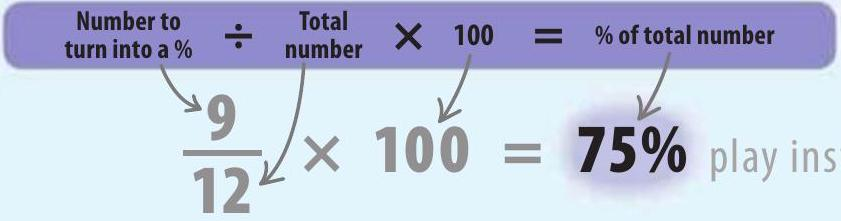
\includegraphics[max width=\textwidth, center]{2025_07_08_04014fa2c17a4b6cdcc6g-064}

Divide the known number by the\\
Multiply the result by 100 to get total number ( $9 \div 12=0.75$ ). the percentage ( $0.75 \times 100=75$ ).\\
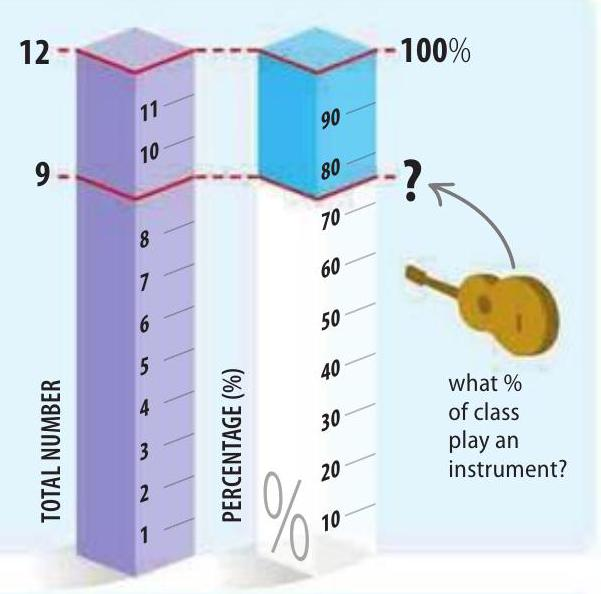
\includegraphics[max width=\textwidth, center]{2025_07_08_04014fa2c17a4b6cdcc6g-064(2)}

\section*{Finding the total number from a \%}
In a class, 7 children make up $35 \%$ of the total. To find the total number of students in the class, divide the known value (7) by the known percentage (35) and multiply by 100.\\
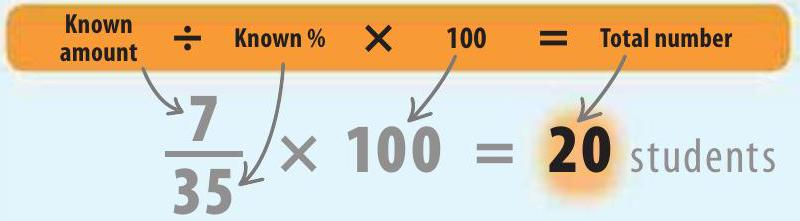
\includegraphics[max width=\textwidth, center]{2025_07_08_04014fa2c17a4b6cdcc6g-064(1)}

Divide the known amount by the\\
Multiply the result by 100 to get known percentage ( $7 \div 35=0.2$ ). the total number ( $0.2 \times 100=20$ ).\\
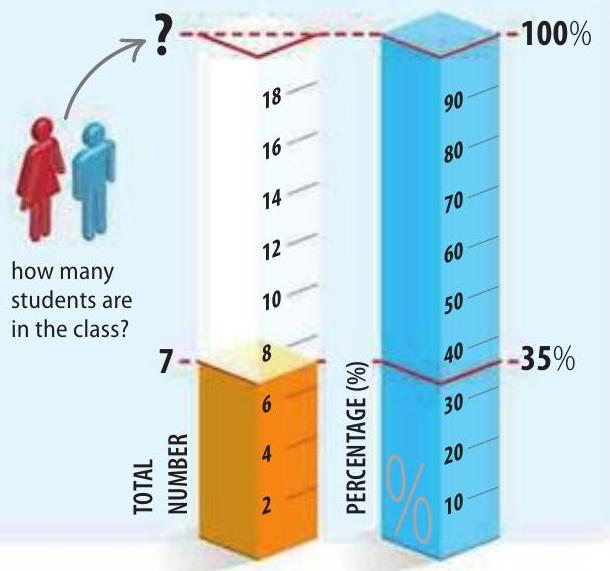
\includegraphics[max width=\textwidth, center]{2025_07_08_04014fa2c17a4b6cdcc6g-064(3)}

\section*{REAL WORLD}
\section*{Percentages}
Percentages are all around us - in shops, in newspapers, on TV - everywhere. Many things in everyday life are measured and compared in percentages - how much an item is reduced in a sale; what the interest rate is on a mortgage or a bank loan; or how efficient a light bulb is by the percentage of electricity it converts to light. Percentages are even used to show how much of the recommended daily intake of vitamins and other nutrients is in food products.\\

\includegraphics[max width=\textwidth, center]{2025_07_08_04014fa2c17a4b6cdcc6g-064(4)}

\section*{PERCENTAGE CHANGE}
If a value changes by a certain percentage, it is possible to calculate the new value. Conversely, when a value changes by a known amount, it is possible to work out the percent increase or decrease compared to the original.

\section*{Finding a new value from a \% increase or decrease}
To find how a 55\% increase or decrease affects the value of 40, first work out 55\%

\begin{center}
\begin{tabular}{|l|l|l|l|l|l|l|l|l|l|l|l|}
\hline
\multicolumn{8}{|l|}{of 40. Then add to or subtract from the original to get the new value.} & 35 & \multirow{2}{*}{} & 90 & \multirow{7}{*}{-55\%} \\
\hline
\multirow{3}{*}{\begin{tabular}{l}
Known \% $\div 100$ \\
Original - \% of total value \\
\end{tabular}} & \multirow{3}{*}{THEN} & \multicolumn{3}{|r|}{Original $\quad+\quad \%$ of total value or - value} & - New value & \multicolumn{2}{|c|}{what is 55\% of 40?} & 30 &  & 10 &  \\
\hline
 &  & 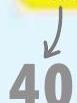
\includegraphics[max width=\textwidth]{2025_07_08_04014fa2c17a4b6cdcc6g-065}
 & 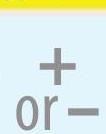
\includegraphics[max width=\textwidth]{2025_07_08_04014fa2c17a4b6cdcc6g-065(1)}
 &  & 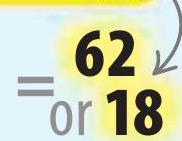
\includegraphics[max width=\textwidth]{2025_07_08_04014fa2c17a4b6cdcc6g-065(4)}
 & 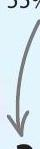
\includegraphics[max width=\textwidth]{2025_07_08_04014fa2c17a4b6cdcc6g-065(3)}
 &  &  &  & 50 &  \\
\hline
 &  &  &  &  &  &  &  & 15 &  & 40 &  \\
\hline
 &  &  &  &  &  &  &  &  &  & 30 &  \\
\hline
Divide the known \% by 100 $(55 \div 100=0.55)$. &  & Add the original value to 22 to find the \% increase, or subtract 22 to find the \% decrease. &  &  &  &  &  & 10 & 
\includegraphics[max width=\textwidth]{2025_07_08_04014fa2c17a4b6cdcc6g-065(2)}
 & 20 &  \\
\hline
 &  &  &  &  &  &  & 童 &  &  & 10 &  \\
\hline
\end{tabular}
\end{center}

\section*{Finding an increase in a value as a \%}
The price of a doughnut in the school canteen has risen 30p - from 99p last year to $\pounds 1.29$ this year. To find the increase as a percent, divide the increase in value (30) by the original value (99) and multiply by 100.\\
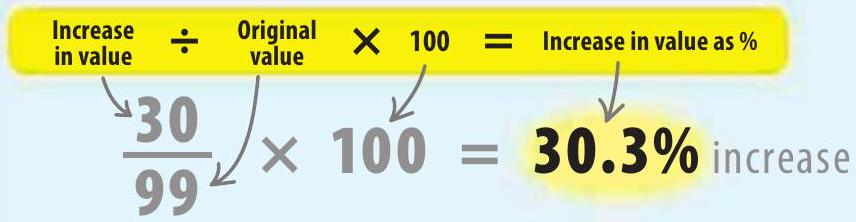
\includegraphics[max width=\textwidth, center]{2025_07_08_04014fa2c17a4b6cdcc6g-065(5)}

Divide the increase in value by the original value ( $30 \div 99=0.303$ ).

Multiply the result by 100 to find the percentage ( $0.303 \times 100=30.3$ ), and round to 3 significant figures.\\
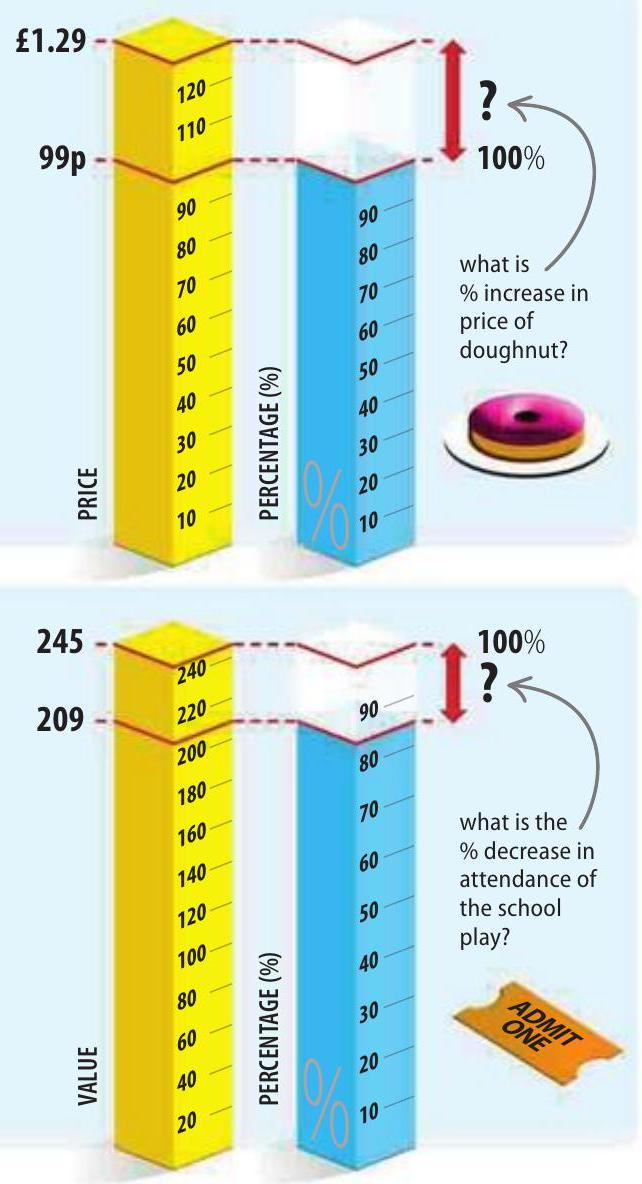
\includegraphics[max width=\textwidth, center]{2025_07_08_04014fa2c17a4b6cdcc6g-065(6)}

\section*{Converting fractions, decimals, and percentages }
\begin{center}
\begin{tabular}{|l|}
\hline
SEE ALSO \\
\hline
《 $\mathbf{4 4 - 4 5}$ Decimals \\
\hline
《8-55 Fractions \\
\hline
स60-63 Percentages \\
\hline
\end{tabular}
\end{center}

\section*{DECIMALS, FRACTIONS, AND PERCENTAGES ARE DIFFERENT WAYS OF WRITING THE SAME NUMBER.}
\section*{The same but different}
Sometimes a number shown one way can be shown more clearly in another way. For example, if 20\% is the mark required to pass an exam, this is the same as saying that $1 / 5$ of the answers in an exam need to be answered correctly to achieve a pass mark or that the minimum score for a pass is 0.2 of the total.

\section*{Changing a decimal into a percentage}
To change a decimal into a percentage, multiply by 100.

$$
0.75 \Rightarrow 75 \%
$$

\begin{center}
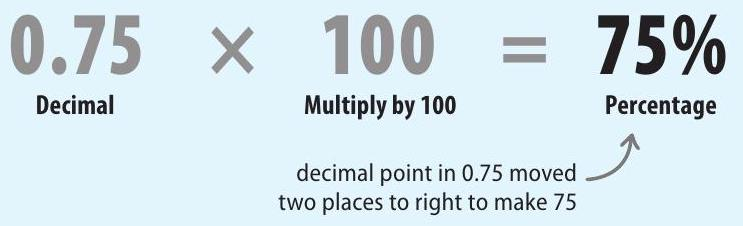
\includegraphics[max width=\textwidth]{2025_07_08_04014fa2c17a4b6cdcc6g-066(1)}
\end{center}

\section*{Changing a percentage into a decimal}
To change a percentage into a decimal, divide it by 100.\\
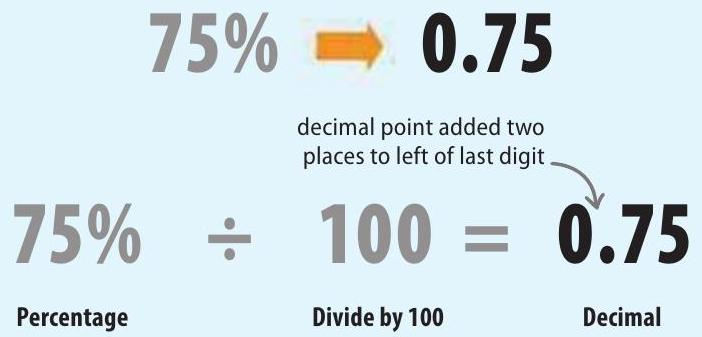
\includegraphics[max width=\textwidth, center]{2025_07_08_04014fa2c17a4b6cdcc6g-066}

\section*{75\%}
\begin{center}
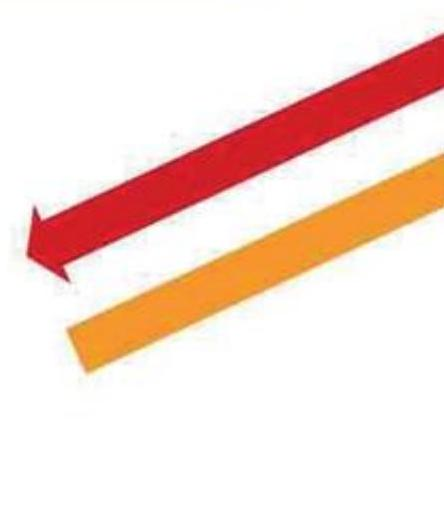
\includegraphics[max width=\textwidth]{2025_07_08_04014fa2c17a4b6cdcc6g-066(2)}
\end{center}

\section*{PERCENTAGE}
A percentage shows a number as a proportion of 100.

\section*{$\triangleright$ All change}
The three ways of writing the same number are shown here: decimal (0.75), fraction (3/4), and percentage (75\%). They look different, but they all represent the same proportion of an amount.

Changing a percentage into a fraction\\
To change a percentage into a fraction, write it as a fraction of 100 and then cancel it down to simplify it, if possible.\\
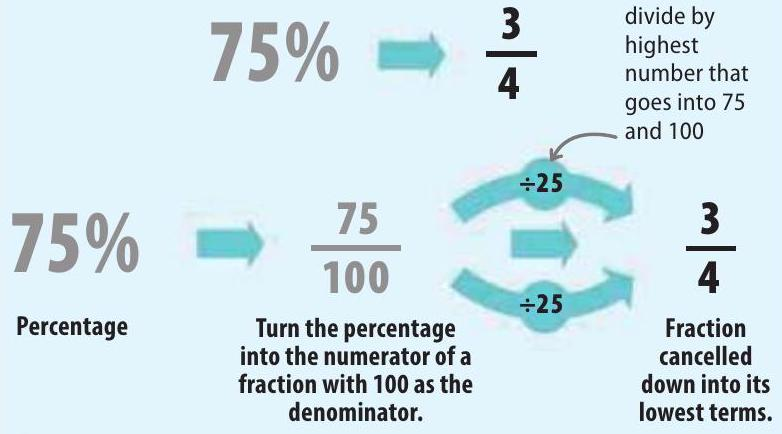
\includegraphics[max width=\textwidth, center]{2025_07_08_04014fa2c17a4b6cdcc6g-066(3)}\\
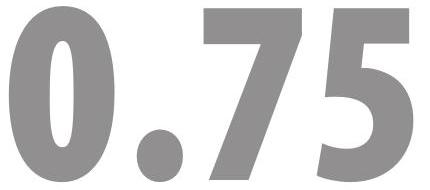
\includegraphics[max width=\textwidth, center]{2025_07_08_04014fa2c17a4b6cdcc6g-067(2)}

\section*{DECIMAL}
A decimal is simply a number that is not whole. It always contains a decimal point.\\
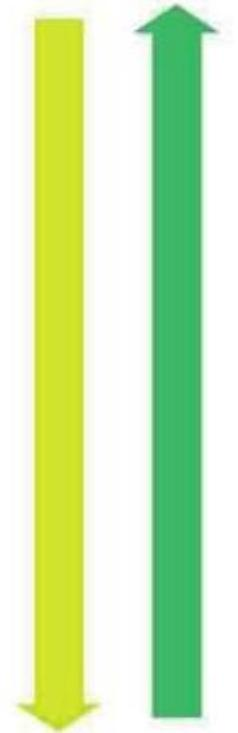
\includegraphics[max width=\textwidth, center]{2025_07_08_04014fa2c17a4b6cdcc6g-067}

FRACTION\\
A fraction shows a number as part of an equally divided whole.

\section*{Changing a fraction into a percentage}
To change a fraction into a percentage, change it to a decimal and then multiply it by 100 .\\
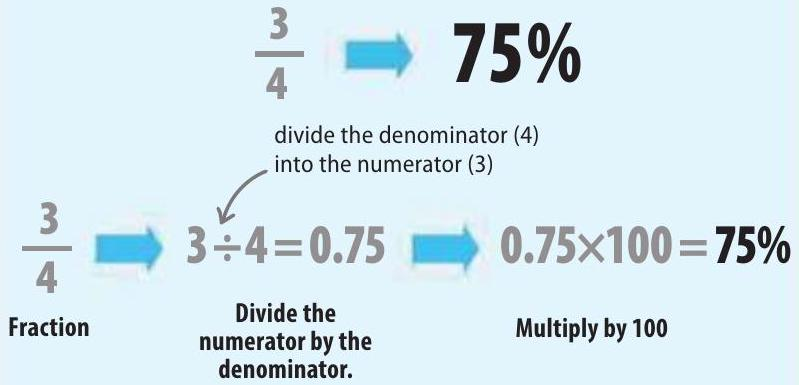
\includegraphics[max width=\textwidth, center]{2025_07_08_04014fa2c17a4b6cdcc6g-067(1)}

\section*{Everyday numbers to remember}
Many decimals, fractions, and percentages are used in everyday life - some of the more common ones are shown here.

\begin{center}
\begin{tabular}{|l|l|l|l|l|l|}
\hline
Decimal & Fraction & \% & Decimal & Fraction & \% \\
\hline
0.1 & 1/10 & 10\% & 0.625 & 5/8 & 62.5\% \\
\hline
0.125 & 1/8 & 12.5\% & 0.666 & 2/3 & 66.7\% \\
\hline
0.25 & 1/4 & 25\% & 0.7 & 7/10 & 70\% \\
\hline
0.333 & 1/3 & 33.3\% & 0.75 & 3/4 & 75\% \\
\hline
0.4 & 2/5 & 40\% & 0.8 & 4/5 & 80\% \\
\hline
0.5 & 1/2 & 50\% & 1 & 1/1 & 100\% \\
\hline
\end{tabular}
\end{center}

\section*{Changing a decimal into a fraction}
First, make the fraction's denominator (its bottom part) 10, 100, 1,000, and so on for every digit after the decimal point.\\
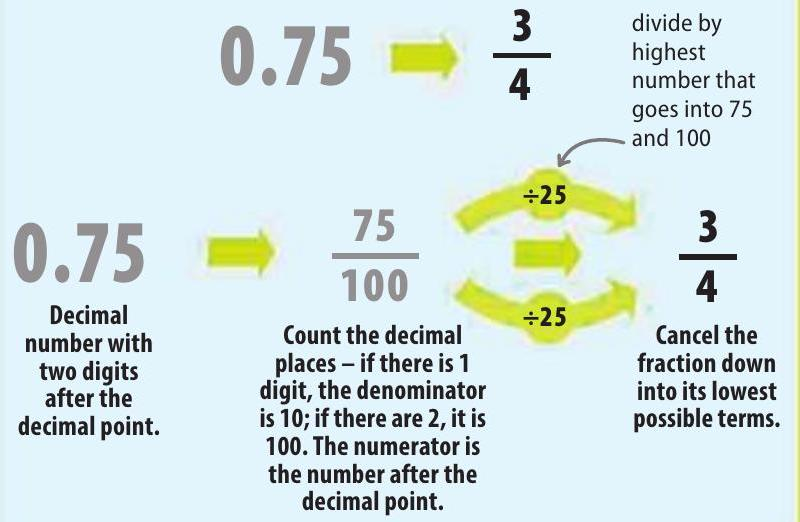
\includegraphics[max width=\textwidth, center]{2025_07_08_04014fa2c17a4b6cdcc6g-067(3)}

\section*{Changing a fraction into a decimal}
Divide the fraction's denominator (its bottom part) into the fraction's numerator (its top part).

\section*{Mental maths}
EVERYDAY PROBLEMS CAN BE SIMPLIFIED SO THAT THEY CAN BE EASILY DONE WITHOUT USING A CALCULATOR.

\begin{center}
\begin{tabular}{|l|}
\hline
SEE ALSO \\
\hline
《18-21 Multiplication \\
\hline
《22-25 Division \\
\hline
Using \\
a calculator \\
\hline
\end{tabular}
\end{center}

\section*{MULTIPLICATION}
Multiplying by some numbers can be easy. For example, to multiply by 10 either add a 0 or move the decimal point one place to the right. Also, to multiply by 20, again multiply by 10 and then double the answer.\\
$\triangleright$ Multiplying by $\mathbf{1 0}$ A sports club hired 2 people last year, but this year it needs to hire 10 times that amount. How many staff members will it recruit this year?\\
\includegraphics[max width=\textwidth, center]{2025_07_08_04014fa2c17a4b6cdcc6g-068}\\
$\triangleleft$ Finding the answer\\
To multiply 2 by 10 add a 0 to the 2. Multiplying 2 people by 10 results in an answer of 20.

\begin{itemize}
  \item Multiplying by 20 A shop is selling t -shirts for the price of $\$ / \pounds 1.20$ each. How much will the price\\
\includegraphics[max width=\textwidth, center]{2025_07_08_04014fa2c17a4b6cdcc6g-068(1)}\\
$\triangleleft$ Finding the answer\\
First multiply the price by 10 , here by moving the decimal point one place to the right, be for 20 t -shirts? and then double that to give the\\
\includegraphics[max width=\textwidth, center]{2025_07_08_04014fa2c17a4b6cdcc6g-068(2)}\\
$\triangleleft$ Finding the answer\\
First multiply the 16 km for one day by 100 , to give $1,600 \mathrm{~km}$ for 100 days, then divide by 4 to give the answer over 25 days.
\end{itemize}

\section*{$\nabla$ Multiplication using decimals}
Decimals appear to complicate the problem, but they can be ignored until the final stage. Here the amount of carpet required to cover a floor needs to be calculated.\\
\includegraphics[max width=\textwidth, center]{2025_07_08_04014fa2c17a4b6cdcc6g-069(3)}

\section*{LOOKING CLOSER}
\section*{Checking the answer}
As 2.9 is almost 3 , multiplying $3 \times 4$ is a good way to check that the calculation to $2.9 \times 4$ is correct.

$$
\begin{aligned}
& \text { symbol for } \\
& \text { approximately } \\
& \text { equal to } \\
& \text { close to real answer of } 11.6 \\
& \text { SO }
\end{aligned}
$$

\begin{center}
\includegraphics[max width=\textwidth]{2025_07_08_04014fa2c17a4b6cdcc6g-069(2)}
\end{center}

First, take away the decimal point from the 2.9 to make the calculation $29 \times 4$.

Change $\mathbf{2 9} \times \mathbf{4}$ to $30 \times \mathbf{4}$, as it is easier to work out. Write $1 \times$ 4 below as it is the difference between $29 \times 4$ and $30 \times 4$.

Subtract 4 (product of $1 \times$ 4) from 120 (product of 30 $\times 4$ ) to give the answer of 116 (product of $29 \times 4$ ).

Move the decimal point one place to the left as it was moved one place to the right in the first step.

\section*{Top tricks}
The multiplication tables of several numbers reveal patterns of multiplications. Here are two good mental tricks to remember when multiplying the 9 and 11 times tables.\\
\includegraphics[max width=\textwidth, center]{2025_07_08_04014fa2c17a4b6cdcc6g-069(1)}

\section*{$\triangle$ Two digits are added together}
The two digits that make up the first 10 multiples of 9 each add up to 9 . The first digit of the multiple (such as 1 , in 18 ) is always 1 less than the multiplier (2).\\
\includegraphics[max width=\textwidth, center]{2025_07_08_04014fa2c17a4b6cdcc6g-069}

\section*{$\triangle$ Digit is written twice}
To multiply by 11, merely repeat the two multipliers together. For example, $4 \times 11$ is two 4 s or 44 . It works all the way up to $9 \times 11=99$, which is 9 written twice.

\section*{DIVISION}
Dividing by 10 or 5 is straightforward. To divide by 10, either delete a 0 or move the decimal point one place to the left. To divide by 5, again divide by 10 and then double the answer.\\
Using these rules, work out the divisions in the following two examples.\\
$\triangleright$ Dividing by 10\\
In this example, 160 travel vouchers are needed to hire a 10-seat mini bus. How many travel vouchers are needed for each of the 10 children to travel on the bus?\\
\includegraphics[max width=\textwidth, center]{2025_07_08_04014fa2c17a4b6cdcc6g-070(1)}

How many each? To find the number of travel vouchers for each child, divide the total of 160 by 10 by deleting a 0 from the 160. It gives the answer of 16 travel vouchers each.

\section*{- Dividing by 5}
The cost of admission to a zoo for a group of five children is 75 tokens. How many tokens are needed for 1 of the 5 children to enter the zoo?\\
\includegraphics[max width=\textwidth, center]{2025_07_08_04014fa2c17a4b6cdcc6g-070}\\
$\triangleleft$ How many each? To find the admission for 1 child, divide the total of 75 by 10 (by moving a decimal point in 75 one place to the left) to give 7.5, and then double that for the answer of 15.

\section*{LOOKING CLOSER}
\section*{Top tips}
There are various mental tricks to help with dividing larger or more complicated numbers. In the three examples below, there are tips on how to check whether very large numbers can be divided by 3,4 , and 9 .

\section*{$\triangleright$ Divisible by 3}
Add together all of the digits in the number. If the total is divisible by 3 , the original number is too.

\section*{$\triangleright$ Divisible by 4}
If the last two digits are taken as one single number, and it is divisible by 4 , the original number is too.\\
$1665233198172 \Rightarrow 1+6+6+5+2+3+3+1+9+8+1+7+2=54$

$123456123456123456=56 \div 4=14 \overbrace{}^{$\begin{tabular}{c}
5 \text{and} 6 \text{seen as} \\
\text{one number:} 56 \\
\end{tabular}$}$

$1643951142 \Rightarrow 1+6+4+3+9+5+1+1+4+2=36=$\begin{tabular}{c}
add together all digits of \\
number, their sum is 36 \\
original number \\
is divisibile by 9 \\
\end{tabular}

\section*{PERCENTAGES}
A useful method of simplifying calculations involving percentages is to reduce one difficult percentage into smaller and easier-to-calculate parts. In the example below, the smaller percentages include 10\% and 5\%, which are easy to work out.

\section*{Adding 17.5 per cent}
Here a shop wants to charge \$/£480 for a new bike. However, the owner of the shop has to add a sales tax of\\
\includegraphics[max width=\textwidth]{2025_07_08_04014fa2c17a4b6cdcc6g-071(2)} 17.5 per cent to the price. How much will it then cost?\\
\includegraphics[max width=\textwidth, center]{2025_07_08_04014fa2c17a4b6cdcc6g-071(3)}

First, write down the percentage price increase required and the original price of the bike.

Next, reduce 17.5\% into the easier stages of 10\%, 5\%, and $2.5 \%$ of $\pounds / \$ 480$, and calculate their values.

The sum of 48,24 , and 12 is 84 , so $\$ / \pounds 84$ is added to $\$ / \pounds 480$ for a price of $\$ / \pounds 564$.

\section*{Switching}
A percentage and an amount can both be "switched", to produce the same result with each switch. For example, $50 \%$ of 10 , which is 5 , is exactly the same as $10 \%$ of 50 , which is 5 again.\\
\includegraphics[max width=\textwidth, center]{2025_07_08_04014fa2c17a4b6cdcc6g-071}

\section*{Progression}
A progression involves dividing the percentage by a number and then multiplying the amount by the same number. For example, $40 \%$ of 10 is 4 . Dividing this $40 \%$ by 2 and multiplying 10 by 2 results in $20 \%$ of 20 , which is also 4 .\\
\includegraphics[max width=\textwidth, center]{2025_07_08_04014fa2c17a4b6cdcc6g-071(1)}

\section*{Rounding off}
THE PROCESS OF ROUNDING OFF INVOLVES REPLACING ONE\\
\includegraphics[max width=\textwidth]{2025_07_08_04014fa2c17a4b6cdcc6g-072(1)} NUMBER WITH ANOTHER TO MAKE IT MORE PRACTICAL TO USE.

\section*{Estimation and approximation}
In many practical situations, an exact answer is not needed, and it is easier to find an estimate based on rounding off (approximation). The general principle of rounding off is that a number at or above the midpoint of a group of numbers, such as the numbers 15-19 in the group 10-20, rounds up, while a number below the midpoint rounds down.

\section*{$\nabla$ Rounding to the nearest $\mathbf{1 0}$}
The midpoint between any two 10s is 5 . If the last digit of each number is 5 or over it rounds up, otherwise it rounds down.\\
\includegraphics[max width=\textwidth, center]{2025_07_08_04014fa2c17a4b6cdcc6g-072(2)}\\
if the last digit is below the midpoint, round down\\
\includegraphics[max width=\textwidth, center]{2025_07_08_04014fa2c17a4b6cdcc6g-072(3)}\\
if the last digit is at or above the midpoint, round up\\
\includegraphics[max width=\textwidth, center]{2025_07_08_04014fa2c17a4b6cdcc6g-072(4)}

LOOKING CLOSER

\section*{Approximately equal}
Many measurements are given as approximations, and numbers are sometimes rounded to make them easier to use. An "approximately equals" sign is used to show when numbers have been rounded up or down. It looks similar to a normal equals sign (=) but with curved instead of straight lines.\\
\includegraphics[max width=\textwidth, center]{2025_07_08_04014fa2c17a4b6cdcc6g-072}

\section*{$31 \approx 30$ and $187 \approx 200$}
\section*{$\triangle$ Approximately equal to}
The "approximately equals" sign shows that the two sides of the sign are approximately equal instead of equal. So 31 is approximately equal to 30 , and 187 is approximately equal to 200.

\section*{Decimal places}
Any number can be rounded to the appropriate number of decimal places. The choice of how many decimal places depends on what the number is used for and how exact an end result is required.\\
\includegraphics[max width=\textwidth, center]{2025_07_08_04014fa2c17a4b6cdcc6g-073(2)}

\section*{LOOKING CLOSER}
\section*{How many decimal places?}
The more decimal places, the more accurate the number. This table shows the accuracy that different numbers of decimal places represent. For example, a distance in kilometres to 3 decimal places would be accurate to a thousandth of a kilometre, which is equal to a metre.

\begin{center}
\begin{tabular}{|c|c|c|}
\hline
\begin{tabular}{c}
Decimal \\
places \\
\end{tabular} & Rounded to & Example \\
\hline
1 & $1 / 10$ & 1.1 km \\
\hline
2 & $1 / 100$ & 1.14 km \\
\hline
3 & $1 / 1000$ & 1.135 km \\
\hline
\end{tabular}
\end{center}

\section*{Significant figures}
A significant figure in a number is a digit that counts. The digits 1 to 9 are always significant, but 0 is not. However, 0 becomes significant when it occurs between two significant figures, or if an exact answer is needed.

Real value anywhere\\
\includegraphics[max width=\textwidth]{2025_07_08_04014fa2c17a4b6cdcc6g-073} between 150-249\\
\includegraphics[max width=\textwidth, center]{2025_07_08_04014fa2c17a4b6cdcc6g-073(1)}

5 significant figures ( 5 s.f.)\\
\includegraphics[max width=\textwidth, center]{2025_07_08_04014fa2c17a4b6cdcc6g-073(3)}\\
$\triangleleft$ Significant zeros The answer 200 could be the result of rounding to 1,2 , or 3 significant figures (s.f.). Below each example is the range in which its true value lies.

\section*{Using a Calculator}
CALCULATORS ARE MACHINES THAT WORK OUT THE ANSWERS

Calculators are designed to make maths easier，but there are a few things to be aware of when using them．

\section*{Introducing the calculator}
A modern calculator is a handheld electronic device that is used to find the answers to mathematical problems．Most calculators are operated in a similar way（as described here），but it may be necessary to read the instructions for a particular model．

\section*{Using a calculator}
Be careful that functions are entered in the correct order， or the answers the calculator gives will be wrong．

For example，to find the answer to the sum：\\
$(\mathbf{7}+\mathbf{2}) \times \mathbf{9}=$\\
Enter these keys，making sure to include all parts of the sum，including the brackets．\\
$07+20 \times 9=81$\\
Not\\
$7+2 \times 9=\mathbf{2 5}^{\leftarrow}$ calculator does sum $2 \times 9=18$ ， then $18+7=25$

\section*{Estimating answers}
Calculators can only give answers according to the keys that have been pressed．It is useful to have an idea of what answer to expect as a small mistake can give a very wrong answer．

For example\\
\includegraphics[max width=\textwidth, center]{2025_07_08_04014fa2c17a4b6cdcc6g-074(2)}\\
must be close to this would give the\\
\includegraphics[max width=\textwidth, center]{2025_07_08_04014fa2c17a4b6cdcc6g-074(1)}

So if the calculator gives the answer $\mathbf{4 0 , 7 8 8}$ it is clear that the sum has not been entered correctly－the sum entered had one＂0＂missing from what was intended：\\
\includegraphics[max width=\textwidth, center]{2025_07_08_04014fa2c17a4b6cdcc6g-074}

\section*{FREQUENTLY USED KEYS}
\section*{囲－ON}
ON\\
This button turns the calculator on－most calculators turn themselves off automatically if they are left unused for a certain period of time．

\section*{1}
\section*{Number pad}
This contains the basic numbers that are needed for maths．These buttons can be used individually or in groups to create larger numbers．

\section*{母－}
\section*{Standard arithmetic keys}
These cover all the basic mathematical functions： multiplication，division，addition，and subtraction，as well as the essential equals sign．\\
$\square$ Decimal point\\
This key works in the same way as a written decimal point－it separates whole numbers from decimals．It is entered in the same way as any of the number keys．

\section*{AC}
\section*{Cancel}
The cancel key clears all recent entries from the memory．This is useful when starting a new calculation，as it makes sure no unwanted values are retained．

\section*{DEL}
Delete\\
This clears the last value that was entered into the calculator，rather than wiping everything from the memory． It is sometimes labelled＂CE＂（clear entry）．

\section*{RCL}
\section*{Recall button}
This recalls a value from the calculator＇s memory－ it is useful for sums with many parts that use numbers or stages from earlier in the working out．\\
\includegraphics[max width=\textwidth, center]{2025_07_08_04014fa2c17a4b6cdcc6g-075(6)}

\section*{FUNCTION KEYS}
\begin{center}
\includegraphics[max width=\textwidth]{2025_07_08_04014fa2c17a4b6cdcc6g-075(2)}
\end{center}

\section*{Cube}
This is a short cut to cubing a number, without having to key in a number multiplied by itself, and then multiplied by itself again. Key in the number to be cubed, then press this button.\\
\includegraphics[max width=\textwidth, center]{2025_07_08_04014fa2c17a4b6cdcc6g-075}

ANS\\
Pressing this key gives the answer to the last sum that was entered. It is useful for sums with many steps.\\
\includegraphics[max width=\textwidth, center]{2025_07_08_04014fa2c17a4b6cdcc6g-075(4)}

Square root\\
This finds the positive square root of a positive number. Press the square root button first, then the number, and then the equals button.\\
\includegraphics[max width=\textwidth, center]{2025_07_08_04014fa2c17a4b6cdcc6g-075(3)}

\section*{Square}
A short cut to squaring a number, without having to key in the number multiplied by itself. Just key in the number then this button.\\
\includegraphics[max width=\textwidth, center]{2025_07_08_04014fa2c17a4b6cdcc6g-075(1)}

\section*{Exponent}
Allows a number to be raised to a power. Enter the number, then the exponent button, then the power.\\
\includegraphics[max width=\textwidth, center]{2025_07_08_04014fa2c17a4b6cdcc6g-075(5)}

Negative\\
Use this to make a number negative. It is usually used when the first number in a sum is negative.

\section*{$\triangle$ Scientific calculator}
A scientific calculator has many functions - a standard calculator usually only has the number pad, standard arithmetic keys, and one or two other, simpler functions, such as percentages. The keys shown here allow for more advanced maths.\\
$\square$ Brackets\\
These work in the same way as surrounding a part of a sum with brackets - they make sure the order of operations is correct.

\section*{KNOWING HOW MONEY WORKS IS IMPORTANT FOR MANAGING YOUR PERSONAL FINANCES.}
Personal finance includes paying tax on income, gaining interest on savings, or paying interest on loans.

\begin{center}
\begin{tabular}{|l|}
\hline
SEE ALSO \\
\hline
《34-35 Positive and \\
negative numbers \\
\hline
Business finance \\
\hline
Formulas \\
\hline
\end{tabular}
\end{center}

\section*{Tax}
Tax is a fee charged by a government on a product, income, or activity. Governments collect the money they need to provide services, such as schools and defence, by taxing individuals and companies. Individuals are taxed on what they earn - income tax - and also on some things they buy.\\
\includegraphics[max width=\textwidth, center]{2025_07_08_04014fa2c17a4b6cdcc6g-076}

\section*{FINANCIAL TERMS}
Financial words often seem complicated, but they are easy to understand. Knowing what the important ones mean will enable you to manage your finances by helping you to understand what you have to pay and the money you will receive.

\begin{center}
\begin{tabular}{|l|l|}
\hline
Bank account & This is the record of whatever a person borrows from or saves with the bank. Each account holder has a numeric password called a personal identification number (PIN), which should never be revealed to anyone. \\
\hline
Credit & Credit is money that is borrowed - for example, on a 4-year pay-back agreement or as an overdraft from the bank. It always costs to borrow money. The money paid to borrow from a bank is called interest. \\
\hline
Income & This is the money that comes to an individual or family. This can be provided by the wages that are paid for employment. Sometimes it comes from the government in the form of an allowance or direct payment. \\
\hline
Interest & This is the cost of borrowing money or the income received when saving with a bank. It costs more to borrow money from a bank than the interest a person would receive from the bank by saving the same amount. \\
\hline
Mortgage & A mortgage is an agreement to borrow money to buy a home. A bank lends the money for the purchase and this is paid back, usually over a long period of time, together with interest on the loan and other charges. \\
\hline
Savings & There are many forms of savings. Money can be saved in a bank to earn interest. Saving through a pension plan involves making regular payments to ensure an income after retirement. \\
\hline
Break-even & Break-even is the point where the cost, or what a company has spent, is equal to revenue, which is what the company has earned - at break-even the company makes neither a profit nor a loss. \\
\hline
Loss & Companies make a loss if they spend more than they earn - if it costs them more to produce their product than they earn by selling it. \\
\hline
Profit & Profit is the part of a company's income that is left once their costs have been paid - it is the money "made" by a company. \\
\hline
\end{tabular}
\end{center}

\section*{INTEREST}
Banks pay interest on the money that savers invest with them (capital), and charge interest on money that is borrowed from them. Interest is given as a percentage, and there are two types, simple and compound.

\section*{Simple interest}
This is interest paid only on the sum of money that is first saved with the bank. If $\pounds 10,000$ is put in a bank account with an interest rate of $3 \%$, the amount will increase by the same figure each year.

$$
\text { Interest }=\frac{P \times R \times T}{100}
$$

\begin{center}
\includegraphics[max width=\textwidth]{2025_07_08_04014fa2c17a4b6cdcc6g-077(1)}
\end{center}

Substitute the values in the formula to work out the value of the interest for the year.\\
\includegraphics[max width=\textwidth, center]{2025_07_08_04014fa2c17a4b6cdcc6g-077(4)}

After one year, this is the total amount of money in the saver's bank account.

\section*{Simple interest formula}
To find the simple interest made in a given year, substitute real values into this formula.\\
\includegraphics[max width=\textwidth, center]{2025_07_08_04014fa2c17a4b6cdcc6g-077(2)}\\
\includegraphics[max width=\textwidth, center]{2025_07_08_04014fa2c17a4b6cdcc6g-077}

After two years the interest is the same as the first year, as it is only paid on the initial investment.

\section*{Compound interest}
This is where interest is paid on the money invested and any interest that is earned on that money. If $\pounds 10,000$ is paid into a bank account with an interest rate of $3 \%$, then the amount will increase as follows.\\
\includegraphics[max width=\textwidth, center]{2025_07_08_04014fa2c17a4b6cdcc6g-077(5)}

Substitute the values in the formula to work out the total for the first year.

After one year the total interest earned is the same as that earned with simple interest (see above).

\section*{$\triangle$ Compound interest formula}
 To find the compound interest made in a given year, substitute values into this formula.\begin{center}
\includegraphics[max width=\textwidth]{2025_07_08_04014fa2c17a4b6cdcc6g-077(6)}
\end{center}

Substitute the values in the formula to work out the total for the second year.\\
\includegraphics[max width=\textwidth, center]{2025_07_08_04014fa2c17a4b6cdcc6g-077(3)}

After two years there is a greater increase because interest is also earned on previous interest.

\section*{Business Finance}
\section*{BUSINESSES AIM TO MAKE MONEY, AND MATHS PLAYS AN IMPORTANT PART IN ACHIEVING THIS AIM.}
The aim of a business is to turn an idea or a product into a profit, so that the business earns more money than it spends.

\section*{What a business does}
Businesses take raw materials, process them, and sell the end product. To make a profit, the business must sell its end product at a price higher than the total cost of the materials and the manufacturing or production. This example shows the basic stages of this process using a cake-making business.

\begin{center}
\begin{tabular}{|l|l|}
\hline
\multicolumn{2}{|l|}{SEE ALSO} \\
\hline\hline
X74-75 Personal finance &  \\
\hline
Pie charts & $\mathbf{2 1 0}$-211 \\
\hline
Line graphs & $\mathbf{2 1 2 - 2 1 3} \boldsymbol{\text { 女 }}$ \\
\hline
\end{tabular}
\end{center}

\begin{itemize}
  \item Making cakes
\end{itemize}

This diagram shows how a cake-making business processes inputs to produce an output.\\
\includegraphics[max width=\textwidth, center]{2025_07_08_04014fa2c17a4b6cdcc6g-078(1)}

\section*{1}
\section*{INPUTS}
Inputs are raw materials that are used in making a product. For cake making, the inputs would include the ingredients such as flour, eggs, butter, and sugar.

\section*{$\triangle$ Costs}
Costs are incurred at the input stage, as the raw materials have to be paid for. The same costs occur every time a new batch of cakes is made.

\section*{Revenue and profit}
There is an important difference between revenue and profit. Revenue is the money a business makes when it sells its product. Profit is the difference between revenue and cost it is the money that the business has "made".\\
\includegraphics[max width=\textwidth, center]{2025_07_08_04014fa2c17a4b6cdcc6g-078}\\
some costs are fixed, and the money is spent however much of the product is sold so costs do not start at 0

\section*{$\triangleright$ Cost graph}
This graph shows where a business begins to make a profit: where its revenue is greater than its costs.\\
\includegraphics[max width=\textwidth, center]{2025_07_08_04014fa2c17a4b6cdcc6g-078(2)}\\
\includegraphics[max width=\textwidth, center]{2025_07_08_04014fa2c17a4b6cdcc6g-079}\\
\includegraphics[max width=\textwidth, center]{2025_07_08_04014fa2c17a4b6cdcc6g-080}

Geometry

\section*{$\Delta$ What is geometry?}
GEOMETRY IS THE BRANCH OF MATHEMATICS CONCERNED WITH LINES, ANGLES, SHAPES, AND SPACE.

Geometry has been important for thousands of years, its practical uses include working out land areas, architecture, navigation, and astronomy. It is also an area of mathematical study in its own right.

\section*{Lines, angles, shapes, and space}
Geometry includes topics such as lines, angles, shapes (in both two and three dimensions), areas, and volumes, but also subjects like movements in space, such as rotations and reflections, and coordinates.\\
\includegraphics[max width=\textwidth, center]{2025_07_08_04014fa2c17a4b6cdcc6g-082(2)}

Angles\\
An angle is formed when two lines meet at a point. The size of an angle is the amount of turn between the two lines, measured in degrees.\\
\includegraphics[max width=\textwidth, center]{2025_07_08_04014fa2c17a4b6cdcc6g-082(1)}

Circle\\
A circle is a continuous line that is always the same distance from a central point. The length of the line is the circumference. The diameter runs from one side to the other through the centre. The radius runs from the centre to the circumference.\\
\includegraphics[max width=\textwidth, center]{2025_07_08_04014fa2c17a4b6cdcc6g-082(3)}

Lines that are parallel are the same distance apart along their entire length, and never meet, even if they are extended.

\section*{REAL WORLD}
\section*{Geometry in nature}
Although many people think of geometry as a purely mathematical subject, geometric shapes and patterns are widespread in the natural world. Perhaps the best-known examples are the hexagonal shapes of honeycomb cells in a beehive and of snowflakes, but there are many other examples of natural geometry. For instance, water droplets, bubbles, and planets are all roughly spherical.

Crystals naturally form various polyhedral\\
\includegraphics[max width=\textwidth]{2025_07_08_04014fa2c17a4b6cdcc6g-082} able salt has cubic crystals, and quartz often forms crystals in the shape of a six-sided prism with pyramid shaped ends.

\section*{$\triangleleft$ Honeycomb cells}
Cells of honeycomb are naturally hexagons, which can fit together (tessellate) without leaving any space between them.

\section*{LOOKING CLOSER}
\section*{Graphs and geometry}
Graphs link geometry with other areas of mathematics. Plotting lines and shapes in graphs with coordinates makes it possible to convert them into algebraic expressions, which can then be manipulated mathematically. The reverse is also true: algebraic expressions can be shown on a graph, enabling them to be manipulated using the rules of geometry. Graphical representations of objects enables positions to be given to them, which makes it possible to apply vectors and calculate the results of movements, such as rotations and translations.\\
\includegraphics[max width=\textwidth, center]{2025_07_08_04014fa2c17a4b6cdcc6g-083(2)}

\section*{$\checkmark$ Graph}
The graph here shows a right-angled triangle, ABC , plotted on a graph. The vertices (corners) have the coordinates $\mathrm{A}=(1,1)$, $B=(1,5.5)$, and $C=(4,1)$.\\
\includegraphics[max width=\textwidth, center]{2025_07_08_04014fa2c17a4b6cdcc6g-083}

\section*{Triangle}
A triangle is a three-sided, twodimensional polygon. All triangles have three internal angles that add up to $180^{\circ}$.\\
\includegraphics[max width=\textwidth, center]{2025_07_08_04014fa2c17a4b6cdcc6g-083(4)}

Cube\\
A cube is a three-dimensional polygon in which all its edges are the same length.\\
Like other cuboids, a cube has 6 faces, 12 edges, and 8 vertices (corners).\\
\includegraphics[max width=\textwidth, center]{2025_07_08_04014fa2c17a4b6cdcc6g-083(1)}

\section*{$\triangle$ Square}
A square is a four-sided polygon, or quadrilateral, in which all four sides are the same length and all four internal angles are right angles $\left(90^{\circ}\right)$.\\
\includegraphics[max width=\textwidth, center]{2025_07_08_04014fa2c17a4b6cdcc6g-083(3)}

\section*{Sphere}
A sphere is a perfectly round threedimensional shape in which every point on its surface is the same distance from the centre; this distance is the radius.

\section*{Tools in geometry}
\section*{MATHEMATICAL INSTRUMENTS ARE NEEDED FOR MEASURING AND DRAWING IN GEOMETRY．}
\section*{Tools used in geometry}
Tools are vital to measure and construct geometric shapes accurately．The essential tools are a ruler，a compass，and a protractor．A ruler is used for measuring，and to draw straight lines．A compass is used to draw a whole circle or a part of a circle－ called an arc．A protractor is used to measure and draw angles．

\section*{Using a compass}
A tool for drawing circles and arcs，a compass is made up of two arms attached at one end．To use a compass，hold the arm ending in a point still，while pivoting the other arm，holding a pencil，around it．The point becomes the centre of the circle．\\
$\nabla$ Drawing a circle when given the radius\\
Set the distance between the arms of a compass to the given radius，then draw the circle．\\
\includegraphics[max width=\textwidth, center]{2025_07_08_04014fa2c17a4b6cdcc6g-084(4)}

Use a ruler to set the arms of the compass to the given radius．\\
\includegraphics[max width=\textwidth, center]{2025_07_08_04014fa2c17a4b6cdcc6g-084(5)}

With the compass set to the radius，hold the point down and drag the pencil around．\\
\includegraphics[max width=\textwidth, center]{2025_07_08_04014fa2c17a4b6cdcc6g-084(3)}

\begin{center}
\begin{tabular}{|l|lr|}
\hline
\multicolumn{2}{|l|}{Angles} & $\mathbf{8 4 - 8 5}$ 〉 \\
\hline
Constructions & $\mathbf{1 1 0 - 1 1 3}$ 〉 &  \\
\hline
Circles & $\mathbf{1 3 8 - 1 3 9}$ 〉 &  \\
\hline
\end{tabular}
\end{center}

$\nabla$ Drawing a circle when given its centre and one point on the circumference\\
Put the point of the compass where the centre is marked and extend the other arm so that the tip of the pencil touches the point on the circumference．Then，draw the circle．\\
\includegraphics[max width=\textwidth, center]{2025_07_08_04014fa2c17a4b6cdcc6g-084}

Set the compass to the distance between the two points．\\
\includegraphics[max width=\textwidth, center]{2025_07_08_04014fa2c17a4b6cdcc6g-084(7)}

Hold the point of the compass down and draw a circle through the point．

\section*{$\nabla$ Drawing arcs}
Sometimes only a part of a circle－an arc－is required．Arcs are often used as guides to construct other shapes．\\
\includegraphics[max width=\textwidth, center]{2025_07_08_04014fa2c17a4b6cdcc6g-084(1)}

Draw a line and mark the ends with a point－one will be the centre of the arc， the other a point on its circumference．\\
\includegraphics[max width=\textwidth, center]{2025_07_08_04014fa2c17a4b6cdcc6g-084(2)}

Set the compass to the length of the line－the radius of the arc－and hold it on one of the points to draw the first arc．\\
\includegraphics[max width=\textwidth, center]{2025_07_08_04014fa2c17a4b6cdcc6g-084(6)}

Draw a second arc by holding the point of the compass on the other point．The intersection is equidistant from $A$ and $B$ ．

\section*{Using a ruler}
A ruler can be used to measure straight lines and the distances between any two points. A ruler is also necessary for setting the arms of a compass to a given distance.\\
\includegraphics[max width=\textwidth, center]{2025_07_08_04014fa2c17a4b6cdcc6g-085(7)}\\
$\triangleleft$ Measuring lines\\
Use a ruler to measure straight lines or the distance between any two given points.\\
$\triangleright$ Drawing lines\\
A ruler is also used as a straight edge when drawing lines between two points.\\
\includegraphics[max width=\textwidth, center]{2025_07_08_04014fa2c17a4b6cdcc6g-085(9)}

\section*{Other tools}
Other tools may prove useful when creating drawings and diagrams in geometry.\\
\includegraphics[max width=\textwidth, center]{2025_07_08_04014fa2c17a4b6cdcc6g-085(4)}

\section*{Set square}
A set square looks like a right-angled triangle and is used for drawing parallel lines. There are two types of set square, one has interior angles $90^{\circ}, 40^{\circ}$ and $45^{\circ}$, the other $90^{\circ}, 60^{\circ}$, and 30 .\\
\includegraphics[max width=\textwidth, center]{2025_07_08_04014fa2c17a4b6cdcc6g-085(6)}

\section*{$\triangle$ Calculator}
A calculator provides a number of key options for geometry calculations. For example, functions such as Sine can be used to work out the unknown angles of a triangle.

\section*{Using a protractor}
A protractor is used to measure and draw angles. It is usually made of transparent plastic, which makes it easier to place the centre of the protractor over the point of the angle. When measuring an angle, always use the scale starting with zero.\\
\includegraphics[max width=\textwidth, center]{2025_07_08_04014fa2c17a4b6cdcc6g-085(10)}

\section*{$\nabla$ Measuring angles}
Use a protractor to measure any angle formed by two lines that meet at a point.\\
\includegraphics[max width=\textwidth, center]{2025_07_08_04014fa2c17a4b6cdcc6g-085(1)}

Extend the lines if necessary to make reading easier.\\
\includegraphics[max width=\textwidth, center]{2025_07_08_04014fa2c17a4b6cdcc6g-085(5)}

Place the protractor over the angle and read the angle measurement, making sure to read up from zero.\\
\includegraphics[max width=\textwidth, center]{2025_07_08_04014fa2c17a4b6cdcc6g-085(8)}

The other scale measures the external angle.

\section*{$\nabla$ Drawing angles}
When given the size of an angle, use a protractor to measure and draw the angle accurately.\\
\includegraphics[max width=\textwidth, center]{2025_07_08_04014fa2c17a4b6cdcc6g-085(2)}

Draw a line and mark a point on it.\\
\includegraphics[max width=\textwidth, center]{2025_07_08_04014fa2c17a4b6cdcc6g-085}

Place the protractor on the line with its centre over the point. Read the degrees up from zero to mark the point.\\
\includegraphics[max width=\textwidth, center]{2025_07_08_04014fa2c17a4b6cdcc6g-085(3)}

Draw a line through the two points, and mark the angle.

\section*{$\Delta$ Angles}
\section*{AN ANGLE IS FORMED WHEN TWO LINES MEET AT A COMMON POINT.}
\begin{center}
\begin{tabular}{|l|r|}
\hline
\multicolumn{2}{|l|}{SEE ALSO} \\
\hline
\begin{tabular}{|l|}
\hline
$\mathbf{8 2 - 8 3}$ Tools in \\
geometry \\
\end{tabular} &  \\
\hline
Straight lines & $\mathbf{8 6 - 8 7} \boldsymbol{)}$ \\
\hline
Bearings & $\mathbf{1 0 8 - 1 0 9} \boldsymbol{>}$ \\
\hline
\end{tabular}
\end{center}

Angles show the amount two lines "turn" as they extend in different directions away from a common point. This turn is measured in degrees, represented by the symbol ${ }^{\circ}$.

\section*{Measuring angles}
The size of an angle depends on the amount of turn. A whole turn, making one rotation around a circle, is $360^{\circ}$. All other angles are less than $360^{\circ}$.\\
\includegraphics[max width=\textwidth, center]{2025_07_08_04014fa2c17a4b6cdcc6g-086}

The space between these two lines is the angle. An angle can be named with a letter, its value in degrees, or the symbol $\angle$.

\footnotetext{$\triangle$ Turn\\
Here, the turn is anticlockwise, but a turn can also be clockwise.
}
\includegraphics[max width=\textwidth, center]{2025_07_08_04014fa2c17a4b6cdcc6g-086(1)}

\section*{Types of angle}
There are four important types of angle, which are shown below. They are named according to their size.\\
\includegraphics[max width=\textwidth, center]{2025_07_08_04014fa2c17a4b6cdcc6g-087(5)}

\section*{Naming angles}
Angles can have individual names and names that reflect a shared relationship.\\
\includegraphics[max width=\textwidth, center]{2025_07_08_04014fa2c17a4b6cdcc6g-087(1)}\\
$\triangle$ One angle, three names\\
This angle can be written as a, or as $\angle \mathrm{ABC}$, or as $\angle \mathrm{CBA}$.\\
\includegraphics[max width=\textwidth, center]{2025_07_08_04014fa2c17a4b6cdcc6g-087}\\
$\triangle$ Complementary angles Any two angles that add up to $90^{\circ}$ are complementary.\\
\includegraphics[max width=\textwidth, center]{2025_07_08_04014fa2c17a4b6cdcc6g-087(3)}

Any two angles that add up to $180^{\circ}$ are supplementary.

\section*{Angles on a straight line}
The angles on a straight line make up a half turn and so they add up to $180^{\circ}$. In this example, four adjacent angles add up to the $180^{\circ}$ of a straight line.\\
\includegraphics[max width=\textwidth, center]{2025_07_08_04014fa2c17a4b6cdcc6g-087(2)}

$$
\begin{gathered}
a+b+c+d=180^{\circ} \\
20^{\circ}+40^{\circ}+90^{\circ}+30^{\circ}=180^{\circ}
\end{gathered}
$$

\section*{Angles at a point}
The angles surrounding a point, or vertex, make up a whole turn and so they add up to $360^{\circ}$. In this example, five adjacent angles at the same point add up to the $360^{\circ}$ of a complete circle.\\
\includegraphics[max width=\textwidth, center]{2025_07_08_04014fa2c17a4b6cdcc6g-087(4)}

\section*{Straight lines}
\section*{A STRAIGHT LINE IS USUALLY JUST CALLED A LINE. IT IS THE SHORTEST DISTANCE BETWEEN TWO POINTS ON A SURFACE OR IN SPACE.}
\begin{center}
\begin{tabular}{|l|}
\hline
SEE ALSO \\
\hline
《82-83 Tools in geometry \\
\hline
《84-85 Angles \\
\hline
Constructions 110-113 \\
\hline
\end{tabular}
\end{center}

\section*{Points, lines, and planes}
The most fundamental objects in geometry are points, lines, and planes. A point represents a specific position and has no width, height, or length. A line is one dimensional - it has infinite length extending in two opposite directions. A plane is a two-dimensional flat surface extending in all directions.\\
\includegraphics[max width=\textwidth, center]{2025_07_08_04014fa2c17a4b6cdcc6g-088(3)}\\
$\triangle$ Points\\
A point is used to represent a precise location. It is represented by a dot and named with a capital letter.\\
\includegraphics[max width=\textwidth, center]{2025_07_08_04014fa2c17a4b6cdcc6g-088(1)}

\section*{$\triangle$ Line segments}
A line segment has fixed length, so it will have endpoints rather than arrowheads. A line segment is named by its endpoints this is line segment CD.\\
\includegraphics[max width=\textwidth, center]{2025_07_08_04014fa2c17a4b6cdcc6g-088(2)}\\
\includegraphics[max width=\textwidth, center]{2025_07_08_04014fa2c17a4b6cdcc6g-088(4)}

\section*{$\triangle$ Non-parallel lines}
Non-parallel lines are not the same distance apart all the way along; if they are extended they will eventually meet in a point.\\
\includegraphics[max width=\textwidth, center]{2025_07_08_04014fa2c17a4b6cdcc6g-088(5)}

\section*{$\triangle$ Parallel lines}
Parallel lines are two or more lines that never meet, even if extended. Identical arrows are used to indicate lines that are parallel.

\section*{$\triangle$ Transversal}
Any line that intersects two or more other lines, each at a different point, is called a transversal.

\section*{LOOKING CLOSER}
\section*{Parallelograms}
A parallelogram is a four-sided shape with two pairs of opposite sides, both parallel and of equal length.\\
\includegraphics[max width=\textwidth, center]{2025_07_08_04014fa2c17a4b6cdcc6g-088}

\section*{$\triangle$ Parallel sides}
The sides AB and DC are parallel, as are sides BC and AD . The sides AB and BC , and $A D$ and $C D$ are not parallel - shown by the different arrows on these lines.

\section*{Angles and parallel lines}
Angles can be grouped and named according to their relationships with straight lines. When parallel lines are crossed by a transversal, it creates pairs of equal angles - each pair has a different name.\\
$\nabla$ Labelling angles\\
Lines $A B$ and $C D$ are parallel. The angles created by the intersecting transversal line are labelled with lower-case letters.\\
\includegraphics[max width=\textwidth, center]{2025_07_08_04014fa2c17a4b6cdcc6g-089(4)}

\section*{$\triangle$ Corresponding angles}
Angles in the same position in relation to the transversal line and one of a pair of parallel lines, are called corresponding angles. These angles are equal.\\
\includegraphics[max width=\textwidth, center]{2025_07_08_04014fa2c17a4b6cdcc6g-089(5)}

\section*{- Vertically-opposite angles}
When two lines cross, equal angles are formed on opposite sides of the point. These angles are known as vertically-opposite angles.\\
\includegraphics[max width=\textwidth, center]{2025_07_08_04014fa2c17a4b6cdcc6g-089(2)}

\section*{$\triangle$ Alternate angles}
Alternate angles are formed on either side of a transversal between parallel lines. These angles are equal.

\section*{Drawing a parallel line}
Drawing a line that is parallel to an existing line requires a pencil, a ruler, and a protractor.\\
\includegraphics[max width=\textwidth, center]{2025_07_08_04014fa2c17a4b6cdcc6g-089(1)}

Draw a straight line with a ruler. Mark a point - this will be the distance of the new, parallel line from the original line.\\
measure this angle between the original line and the line\\
\includegraphics[max width=\textwidth, center]{2025_07_08_04014fa2c17a4b6cdcc6g-089(3)}

Draw a line through the mark, intersecting the original line. This is the transversal. Measure the angle it makes with the original line.\\
\includegraphics[max width=\textwidth, center]{2025_07_08_04014fa2c17a4b6cdcc6g-089}

Measure the same angle from the transversal. Draw the new line through the mark with a ruler; this line is parallel to the original line.

\section*{2:5: Symmetry}
THERE ARE TWO TYPES OF SYMMETRY REFLECTIVE AND ROTATIONAL.

A shape has symmetry when a line can be drawn that splits the shape exactly into two, or when it can fit into its outline in more than one way.

\section*{Reflective symmetry}
A flat (two-dimensional) shape has reflective symmetry when each half of the shape on either side of a bisecting line (mirror line) is the mirror image of the other half. This mirror line is called a line of symmetry.

\begin{itemize}
  \item Isosceles triangle This shape is symmetrical across a central line - the sides and angles on either side of this line are equal, and the line cuts the base in half at right angles.
\end{itemize}

\section*{Planes of symmetry}
Solid (three-dimensional) shapes can be divided using "walls" known as planes. Solid shapes have reflective symmetry when the two sides of the shape split by a plane are mirror images.\\
\includegraphics[max width=\textwidth, center]{2025_07_08_04014fa2c17a4b6cdcc6g-090(3)}

\begin{center}
\begin{tabular}{|lr|}
\hline
\multicolumn{2}{|l|}{SEE ALSO} \\
\hline
\multicolumn{2}{|l|}{<86-87 Straight lines} \\
\hline
Rotations & $\mathbf{1 0 0}-\mathbf{1 0 1}$ 〉 \\
\hline
Reflections & $\mathbf{1 0 2 - 1 0 3}$ 〉 \\
\hline
\end{tabular}
\end{center}

eral triangle An equilateral triangle has a line of symmetry through the middle of each side - not just the base.\\
$\nabla$ Cuboid\\
Formed by three pairs of rectangles, a cuboid can be divided into two symmetrical shapes in three ways.

\section*{$\nabla$ Lines of symmetry}
These are the lines of symmetry for some flat or two-dimensional shapes. Circles have an unlimited number of lines of symmetry.\\
\includegraphics[max width=\textwidth, center]{2025_07_08_04014fa2c17a4b6cdcc6g-090}

Lines of symmetry of a rectangle\\
\includegraphics[max width=\textwidth, center]{2025_07_08_04014fa2c17a4b6cdcc6g-090(1)}

Lines of symmetry of a square\\
\includegraphics[max width=\textwidth, center]{2025_07_08_04014fa2c17a4b6cdcc6g-090(2)}

Every line through the middle of a circle is a line of symmetry

\section*{Rotational symmetry}
A two-dimensional shape has rotational symmetry when it can be rotated about a point, called the centre of rotation, and still exactly fit its original outline. The number of ways it fits its outline when rotated is called its "order" of rotational symmetry.

\section*{Equilateral triangle}
 An equilateral triangle has rotational symmetry of order 3 - when rotated, it fits its original outline in three different ways. centre of rotation\begin{center}
\includegraphics[max width=\textwidth]{2025_07_08_04014fa2c17a4b6cdcc6g-091(1)}
\end{center}

\section*{Square}
A square has rotational symmetry of order 4 - when rotated around its centre of rotation, it fits its original outline in four different ways.\\
\includegraphics[max width=\textwidth, center]{2025_07_08_04014fa2c17a4b6cdcc6g-091(2)}

\section*{Axes of symmetry}
Instead of a single point as the centre of rotation, a three-dimensional shape is rotated around a line known as its axis of symmetry. It has rotational symmetry if, when rotated, it fits into its original outline.

\section*{$\nabla$ Rectangle-based pyramid}
A rectangle-based pyramid can rotate into two different positions around its axis.\\
a rectangle-based pyramid has one axis of rotational symmetry

\section*{$\nabla$ Cylinder \\
 A cylinder can rotate}
 into an unlimited number of positions around its vertical axis. orical one vertical axis of rotational symmetry\begin{center}
\includegraphics[max width=\textwidth]{2025_07_08_04014fa2c17a4b6cdcc6g-091}
\end{center}

\section*{Coordinates}
COORDINATES GIVE THE POSITION OF A PLACE OR POINT

\section*{Introducing coordinates}
Coordinates come in pairs of numbers or letters, or both. They are always written in brackets separated by a comma. The order in which coordinates are read and written is important. In this example, (E, 1), means four units, or squares on this map, to the right (along the horizontal row) and one square down, or up in some cases, (the vertical column).\\
\includegraphics[max width=\textwidth, center]{2025_07_08_04014fa2c17a4b6cdcc6g-092}

\section*{$\nabla$ City map}
A grid provides a framework for locating places on a map. Every square is identified by two coordinates. A place is found when the horizontal coordinate meets the vertical coordinate. On this city map, the horizontal coordinates are letters and the vertical coordinates are numbers. On other maps only numbers may be used.

\section*{Map reading}
The horizontal coordinate is always given first and the vertical coordinate second. On the map below, a letter and a number are paired together to form a coordinate.\\
\includegraphics[max width=\textwidth, center]{2025_07_08_04014fa2c17a4b6cdcc6g-093(11)}

\begin{center}
\begin{tabular}{|l|l|l|l|l|}
\hline
J & I & $L$ & N & 11 \\
\hline
\includegraphics[max width=\textwidth]{2025_07_08_04014fa2c17a4b6cdcc6g-093(7)}
 & \includegraphics[max width=\textwidth]{2025_07_08_04014fa2c17a4b6cdcc6g-093(2)}
 & School & \includegraphics[max width=\textwidth]{2025_07_08_04014fa2c17a4b6cdcc6g-093(9)}
 & Library \\
\hline
\end{tabular}
\end{center}

FIRST AVENUE\\
\includegraphics[max width=\textwidth, center]{2025_07_08_04014fa2c17a4b6cdcc6g-093(12)}

ELM ROAD

\section*{Using coordinates}
Each place of interest on this map can be found using the given coordinates. Remember when reading this map to first read across (horizontal) and then down (vertical).\\
\includegraphics[max width=\textwidth, center]{2025_07_08_04014fa2c17a4b6cdcc6g-093(6)}\\
$\triangleleft$ Cinema\\
Find the cinema using coordinates (B, 4). Start from square $A$ and move 1 square to the right, then move 4 squares down.\\
\includegraphics[max width=\textwidth, center]{2025_07_08_04014fa2c17a4b6cdcc6g-093(5)}

\section*{$\triangleleft$ Post office}
The coordinates of the post office are (E, 1). Find the horizontal coordinate E then move down 1 square.\\
\includegraphics[max width=\textwidth, center]{2025_07_08_04014fa2c17a4b6cdcc6g-093(4)}\\
$\triangleleft$ Town hall\\
Find the town hall using coordinates (J, 5). From square A, move 9 squares to the right, then move 5 squares down.\\
\includegraphics[max width=\textwidth, center]{2025_07_08_04014fa2c17a4b6cdcc6g-093(1)}

\section*{$\triangleleft$ Leisure centre}
Using the coordinates ( $\mathrm{C}, 7$ ), find the location of the leisure centre. First, find C. Next, find 7 on the vertical column.\\
\includegraphics[max width=\textwidth, center]{2025_07_08_04014fa2c17a4b6cdcc6g-093(10)}

\section*{$\triangleleft$ Library}
The coordinates of the library are ( $\mathrm{N}, 1$ ). Find N first then move down 1 square to locate the library.\\
\includegraphics[max width=\textwidth, center]{2025_07_08_04014fa2c17a4b6cdcc6g-093(8)}

\section*{Hospital}
The hospital can be found using the coordinates (G, 7). To find the horizontal coordinate of G, move 6 squares to the right. Then go down 6 squares to find the vertical coordinate 7.

\section*{$\triangleleft$ Fire station}
Find the fire station using coordinates $(\mathrm{H}, 4)$. Move 7 squares to the right to find $H$, then move 4 squares down.\\
\includegraphics[max width=\textwidth, center]{2025_07_08_04014fa2c17a4b6cdcc6g-093(3)}

\section*{$\triangleleft$ School}
The coordinates of the school are ( $L, 1$ ). First find $L$, then move down 1 square to find the school.

\section*{$\triangleleft$ Shopping centre}
\begin{center}
\includegraphics[max width=\textwidth]{2025_07_08_04014fa2c17a4b6cdcc6g-093}
\end{center}

Using the coordinates ( $\mathrm{D}, 3$ ), find the location of the shopping centre. Find D. Next, find 3 on the vertical column.

\section*{Graph coordinates}
Coordinates are used to identify the positions of points on graphs, in relation to two axes - the $y$ axis is a vertical line, and the $x$ axis a horizontal line. The coordinates of a point are written as its position on the x axis, followed by its position on the y axis, $(\mathrm{x}, \mathrm{y})$.

\section*{Four quadrants}
Coordinates are measured on axes, which cross at a point called the "origin". These axes create four quadrants. There are positive values on the axes above and to the right of the origin, and negative values below and to its left.\\
\includegraphics[max width=\textwidth, center]{2025_07_08_04014fa2c17a4b6cdcc6g-094}\\
\includegraphics[max width=\textwidth, center]{2025_07_08_04014fa2c17a4b6cdcc6g-094(1)}

\section*{Coordinates of a point}
Coordinates give the position of a point on each axis. The first number gives its position on the x axis, the second its position on the $y$ axis.

\section*{Plotting coordinates}
Coordinates are plotted on a set of axes. To plot a given point, first read along to its value on the x axis, then read up or down to its value on the $y$ axis. The point is plotted where the two values cross each other.

$$
\begin{array}{ll}
A=(2,2) & B=(-1,-3) \\
C=(1,-2) & D=(-2,1)
\end{array}
$$

These are four sets of coordinates. Each gives its $x$ value first, followed by its $y$ value. Plot the points on a set of axes.\\
\includegraphics[max width=\textwidth, center]{2025_07_08_04014fa2c17a4b6cdcc6g-094(2)}

To plot each point, look at its $\times$ coordinate (the first number), and read along the $x$ axis from 0 to this number. Then read up or down to its y coordinate (the second number).\\
\includegraphics[max width=\textwidth, center]{2025_07_08_04014fa2c17a4b6cdcc6g-094(3)}

Using squared paper, draw a horizontal line to form the x axis, and a vertical line to be the $y$ axis. Number the axes, with the origin separating the positive and negative values.\\
\includegraphics[max width=\textwidth, center]{2025_07_08_04014fa2c17a4b6cdcc6g-094(4)}

Plot each point in the same way. With negative coordinates, the process is the same, but read to the left instead of right for an $x$ coordinate, and down instead of up for a $y$ coordinate.

\section*{Equation of a line}
Lines that pass through a set of coordinates on a pair of axes can be expressed as equations. For example, on the line of the equation $y=x+1$, any point that lies on the line has a $y$ coordinate that is 1 unit greater than its $x$ coordinate.\\
\includegraphics[max width=\textwidth, center]{2025_07_08_04014fa2c17a4b6cdcc6g-095(2)}

The equation of a line can be found using only a few coordinates. This line passes through the coordinates $(-1,0),(0,1)$, and $(1,2)$, so it is already clear what pattern the points follow.\\
\includegraphics[max width=\textwidth, center]{2025_07_08_04014fa2c17a4b6cdcc6g-095(1)}\\
\includegraphics[max width=\textwidth, center]{2025_07_08_04014fa2c17a4b6cdcc6g-095(4)}

The graph of the equation is of all the points where the $y$ coordinate is 1 greater than the $x$ coordinate $(y=x+1)$. This means that the line can be used to find other coordinates that satisfy the equation.

\section*{World map}
Coordinates are used to mark the position of places on the Earth's surface, using lines of latitude and longitude. These work in the same way as the $x$ and $y$ axes on a graph. The "origin" is the point where the Greenwich Meridian (0 for longitude) crosses the Equator (0 for latitude).\\
\includegraphics[max width=\textwidth, center]{2025_07_08_04014fa2c17a4b6cdcc6g-095}\\
\includegraphics[max width=\textwidth, center]{2025_07_08_04014fa2c17a4b6cdcc6g-095(3)}

Lines of longitude run from the North Pole to the South Pole. Lines of latitude are at right-angles to lines of longitude. The origin is where the Equator (x axis) crosses the Greenwich Meridian (y axis).

The coordinates of a point such as $P$ are found by finding how many degrees East it is from the Meridian and how many degrees North it is from the Equator.

This is how the surface of the Earth is shown on a map. The lines of latitude and longitude work the same way as axes -the vertical lines show longitude and horizontal lines show latitude.

\section*{Vectors}
\section*{A VECTOR IS A LINE THAT HAS SIZE (MAGNITUDE) AND DIRECTION.}
A vector is a way to show a distance in a particular direction. It is often drawn as a line with an arrow on it. The length of the line shows the size of the vector and the arrow gives its direction.\\
\includegraphics[max width=\textwidth, center]{2025_07_08_04014fa2c17a4b6cdcc6g-096(1)}

\begin{center}
\begin{tabular}{|l|l|}
\hline
\multicolumn{2}{|l|}{SEE ALSO} \\
\hline
《90-93 Coordinates &  \\
\hline
Translations & $\mathbf{9 8 - 9 9} \boldsymbol{)}$ \\
\hline
\begin{tabular}{l}
Pythagoras' \\
theorem \\
\end{tabular} & $\mathbf{1 2 8 - 1 2 9} \boldsymbol{)}$ \\
\hline
\end{tabular}
\end{center}

\section*{What is a vector?}
A vector is a distance in a particular direction. Often, a vector is a diagonal distance, and in these cases it forms the diagonal side (hypotenuse) of a right-angled triangle (see pp.128129). The other sides of the triangle determine the vector's length and direction. In the example on the left, a swimmer's path is a vector. The other two sides of the triangle are the distance across to the opposite shore from the starting point, and the distance down from the end point that the swimmer was aiming for to the actual end point where the swimmer reaches the shore.

\section*{Vector of a swimmer}
A man sets out to swim to the opposite shore of a river that is 30 m wide. A current pushes him as he swims, and he ends up 20 m downriver from where he intended. His path is a vector with dimensions 30 across and 20 down.

\section*{Expressing vectors}
In diagrams, a vector is drawn as a line with an arrow on it, showing its size and direction. There are three different ways of writing vectors using letters and numbers.\\
A " $v$ " is a general label for a vector, used\\
even when its size is known. It is often\\
used as a label in a diagram.\\
Another way of representing a vector is\\
by giving its start and end points, with\\
an arrow above them to show direction.\\
The size and direction of the vector can\\
be shown by giving the horizontal\\
units over the vertical units.\\
\includegraphics[max width=\textwidth, center]{2025_07_08_04014fa2c17a4b6cdcc6g-096}

\section*{Direction of vectors}
The direction of a vector is determined by whether its units are positive or negative. Positive horizontal units mean movement to the right, negative horizontal units mean left; positive vertical units mean movement up, and negative vertical units mean down.

\section*{- Movement up and left}
This movement has a vector with negative horizontal units and positive\\
\includegraphics[max width=\textwidth, center]{2025_07_08_04014fa2c17a4b6cdcc6g-097(5)}

\begin{itemize}
  \item Movement up and right
\end{itemize}

This movement has a vector with both sets of units positive.\\
\includegraphics[max width=\textwidth, center]{2025_07_08_04014fa2c17a4b6cdcc6g-097(7)}

\section*{Equal vectors}
Vectors can be identified as equal even if they are in different positions on the same grid, as long as their horizontal and vertical units are equal.\\
\includegraphics[max width=\textwidth, center]{2025_07_08_04014fa2c17a4b6cdcc6g-097(6)}

\section*{$\triangleleft$ Equal vectors}
These two vectors are equal to one another, as they have sides of equal size and direction.\\
\includegraphics[max width=\textwidth, center]{2025_07_08_04014fa2c17a4b6cdcc6g-097}\\
vector given as units across over units down

\section*{$\triangleright$ Equal vectors}
These two vectors are equal to one another because their horizontal and vertical sides are both the same size and have the same direction.

$$
\binom{-1}{-5}
$$

numerical expression of both vectors\\
\includegraphics[max width=\textwidth, center]{2025_07_08_04014fa2c17a4b6cdcc6g-097(4)}

\section*{Magnitude of vectors}
With diagonal vectors, the vector is the longest side (c) of a rightangled triangle. Use Pythagoras' theorem to find the length of a vector from its vertical (a) and horizontal (b) units.\\
\includegraphics[max width=\textwidth, center]{2025_07_08_04014fa2c17a4b6cdcc6g-097(2)}\\
square root\\
\includegraphics[max width=\textwidth, center]{2025_07_08_04014fa2c17a4b6cdcc6g-097(1)}\\
length of vector $\mathrm{c}=6.7$\\
\includegraphics[max width=\textwidth, center]{2025_07_08_04014fa2c17a4b6cdcc6g-097(3)}

Put the vertical and horizontal units of the vector into the formula.

Find the squares by multiplying each value by itself.

Add the two squares. This total equals $c^{2}$ (the square of the vector).

Find the square root of the total value (45) by using a calculator.

The answer is the magnitude (length) of the vector.

\section*{Adding and subtracting vectors}
Vectors can be added and subtracted in two ways. The first is by using written numbers to add the horizontal and vertical values. The second is by drawing the vectors end to end, then seeing what new vector is created.

\section*{Addition}
Vectors can be added in two different ways. Both methods give the same answer.

\section*{- Subtraction}
Vectors can be subtracted in two different ways. Both methods give the same answer.\\
\includegraphics[max width=\textwidth, center]{2025_07_08_04014fa2c17a4b6cdcc6g-098(4)}

\section*{$\triangle$ Adding the parts}
To add vectors numerically, add the two top numbers (the horizontal values) and then the two bottom numbers (the vertical values).\\
first vector, from which second vector is subtracted

$$
\binom{3}{2}-\binom{-1}{2}=\binom{p^{1-2+1}}{0}
$$

\section*{$\triangle$ Subtracting the parts}
To subtract one vector from another, subtract its vertical value from the vertical value of the first vector, then do the same for the horizontal values.\\
\includegraphics[max width=\textwidth, center]{2025_07_08_04014fa2c17a4b6cdcc6g-098(3)}

\section*{$\triangle$ Addition by drawing vectors}
Draw one vector, then draw the second starting from the end point of the first. The answer is the new vector that has been created, from the start of the first vector to the end of the second.\\
\includegraphics[max width=\textwidth, center]{2025_07_08_04014fa2c17a4b6cdcc6g-098}

\section*{$\triangle$ Subtraction by drawing vectors}
Draw the first vector, then draw the second vector reversed, starting from the end point of the first vector. The answer to the subtraction is the vector from the start point to the end point.

\section*{Multiplying vectors}
Vectors can be multiplied by numbers, but not by other vectors. The direction of a vector stays the same if it is multiplied by a positive number, but is reversed if it is multiplied by a negative number. Vectors can be multiplied by drawing or by using their numerical values.

\section*{$\nabla$ Vector a}
Vector a has -4 horizontal units and +2 vertical units. It can be shown as a written vector or a drawn vector, as shown below.\\
\includegraphics[max width=\textwidth, center]{2025_07_08_04014fa2c17a4b6cdcc6g-098(2)}

\section*{$\nabla$ Vector a multiplied by 2}
To multiply vector a by 2 numerically, multiply each of its horizontal and vertical parts by 2 . To multiply it by 2 by drawing, simply extend the original vector by the same length again.

$$
\text { vector a } \frac{2 \times-4=-8}{\binom{-4}{2}}=\binom{-8}{4}
$$

\includegraphics[max width=\textwidth, center]{2025_07_08_04014fa2c17a4b6cdcc6g-098(5)}\\
$\nabla$ Vector a multiplied by $-1 / 2$ To multiply vector a by -1/2 numerically, multiply each of its parts by $-1 / 2$. To multiply it by $-1 / 2$ by drawing, draw a vector half the length and in the opposite direction to a.

$$
\begin{aligned}
& \text { vector a } \overbrace{\frac{1}{2}}^{-1 / 2 \times-4=+2} \backslash \\
& \downarrow=-\frac{1}{2} \times\binom{-4}{2}=\binom{+2}{-1}
\end{aligned}
$$

\begin{center}
\includegraphics[max width=\textwidth]{2025_07_08_04014fa2c17a4b6cdcc6g-098(1)}
\end{center}

\section*{Working with vectors in geometry}
Vectors can be used to prove results in geometry. In this example, vectors are used to prove that the line joining the midpoints of any two sides of a triangle is parallel to the third side of the triangle, as well as being half its length.

First, choose 2 sides of triangle $A B C$, in this example $A B$ and $A C$. Mark these sides as the vectors $a$ and $b$. To get from $B$ to $C$, go along $B A$ and then $A C$, rather than $B C$. $B A$ is the vector $-a$ as it is the opposite of $A B$, and $A C$ is just b. This means vector BC is $-\mathrm{a}+\mathrm{b}$.\\
\includegraphics[max width=\textwidth, center]{2025_07_08_04014fa2c17a4b6cdcc6g-099(3)}

Third, use the vectors $1 / 2 a$ and $1 / 2 b$ to find the length of vector PQ . To get from P to Q go along PA then AQ . PA is the vector $-1 / 2 a$, as it is the opposite of AP, and AQ is already known to be $1 / 2 \mathrm{~b}$. This means vector PQ is $-1 / 2 a+1 / 2 b$.\\
\includegraphics[max width=\textwidth, center]{2025_07_08_04014fa2c17a4b6cdcc6g-099(2)}

Second, find the midpoints of the two sides that have been chosen ( AB and AC ). Mark the midpoint of AB as P , and the midpoint of $A C$ as $Q$. This creates three new vectors: $\mathrm{AP}, \mathrm{AQ}$, and PQ . AP is half the length of vector a , and AQ is half the length of vector b .\\
\includegraphics[max width=\textwidth, center]{2025_07_08_04014fa2c17a4b6cdcc6g-099(1)}

Fourth, make the proof. The vectors PQ and BC are in the same direction and are therefore parallel to each other, so the line PQ (which joins the midpoints of the sides $A B$ and $A C$ ) must be parallel to the line $B C$. Also, vector $P Q$ is half the length of vector $B C$, so the line $P Q$ must be half the length of the line $B C$.\\
\includegraphics[max width=\textwidth, center]{2025_07_08_04014fa2c17a4b6cdcc6g-099}

\section*{Translations}
\section*{A TRANSLATION CHANGES THE POSITION OF A SHAPE．}
A translation is a type of transformation．It moves an object to a new position． The translated object is called an image，and it is exactly the same size and shape as the original object．Translations are written as vectors．

\section*{How translations work}
A translation moves an object to a new position，without making any other changes，for example to size or shape． Here，the triangle named $A B C$ is translated so that its image is the triangle $A_{1} B_{1} C_{1}$ ．This translation is named $T_{1}$ ．The triangle $A_{1} B_{1} C_{1}$ is then translated again and its image is the triangle $A_{2} B_{2} C_{2}$ ．This second translation is named $T_{2}$ ．\\
\includegraphics[max width=\textwidth, center]{2025_07_08_04014fa2c17a4b6cdcc6g-100}

\section*{Writing translations}
Translations are written as vectors. The top number shows the horizontal distance an object moves, while the bottom number shows the vertical distance moved. The two numbers are contained within a set of brackets. Each translation can be numbered - for example $T_{1}$, $T_{2}, T_{3}$ - to make it clear which one is being referred to if more than one translation is shown.

\section*{Direction of translations}
The numbers used to show a translation's vector are positive or negative, depending on which direction the object moved. If it moves to the right or up, it is positive; to the left or down, it is negative.

\section*{$\nabla$ Negative translation}
The rectangle ABCD, moves down and left, so the values in its vector are negative.\\
\includegraphics[max width=\textwidth, center]{2025_07_08_04014fa2c17a4b6cdcc6g-101(3)}

$$
\begin{aligned}
& \text { distance moved } \\
& \text { horizontally (to } \\
& \text { the left) } \\
& \text { distance moved } \\
& \text { vertically } \\
& \text { (downwards) }
\end{aligned}
$$

\section*{$\triangleleft$ Translation $\mathbf{T}_{1}$}
The translation $\mathrm{T}_{1}$ moves rectangle $A B C D$ to the new position $A_{1} B_{1} C_{1} D_{1}$. It is written as the vector shown - both its parts are negative.\\
\includegraphics[max width=\textwidth, center]{2025_07_08_04014fa2c17a4b6cdcc6g-101(2)}

\section*{$\triangle$ Translation $\mathbf{T}_{1}$}
To move triangle $A B C$ to position $A_{1} B_{1} C_{1}$ each point moves 6 units horizontally, but does not move vertically. The vector is written as above.

\section*{$\triangle$ Translation $\mathbf{T}_{2}$}
To move triangle $A_{1} B_{1} C_{1}$ to position $A_{2} B_{2} C_{2}$ each point moves 6 units horizontally, then moves 2 units vertically. The vector is written as above.

\section*{LOOKING CLOSER}
\section*{Tessellations in action}
A tessellation is a pattern created using shapes to cover a surface without leaving any gaps. Two shapes can be tessellated with themselves using only translation (and no rotation) - the square and the regular hexagon. To tessellate a hexagon using translation requires 6 different translations; to tessellate a square requires 8.\\
\includegraphics[max width=\textwidth, center]{2025_07_08_04014fa2c17a4b6cdcc6g-101(1)}

\section*{Hexagons}
Each of the hexagons around the outside is a translated image of the central hexagon. The tessellation continues in the same way.\\
\includegraphics[max width=\textwidth, center]{2025_07_08_04014fa2c17a4b6cdcc6g-101}

\section*{$\triangle$ Squares}
Each of the squares around the edge is a translated image of the central square. The tessellation continues in the same way.

\section*{Rotations}
\section*{A ROTATION IS A TYPE OF TRANSFORMATION THAT TAKES AN OBJECT AND MOVES IT ABOUT A GIVEN POINT.}
The point around which a rotation occurs is called the centre of rotation, the distance a shape turns is called the angle of rotation.

\begin{center}
\begin{tabular}{|l|}
\hline
SEE ALSO \\
\hline
《84-85 \\
\hline
X90-93 \\
\hline
《98-99 Coordinates \\
\hline
Reflections \\
\hline
Enlargements \\
\hline
Constructions \\
\hline
\end{tabular}
\end{center}

\section*{Properties of a rotation}
Rotations occur around a fixed point called the centre of rotation, and are measured by angles. Any point on an original object and the corresponding point on its rotated image will be exactly the same distance from the centre of rotation. The centre of rotation can sit inside, outside, or on the outline of an object. A rotation can be drawn, or the centre and angle of an existing rotation found, using a compass, ruler, and protractor.

\begin{itemize}
  \item Rotation about a point
\end{itemize}

This rectangle is rotated about a point outside its outline. If it is rotated through $360^{\circ}$ it returns to its starting position.\\
\includegraphics[max width=\textwidth, center]{2025_07_08_04014fa2c17a4b6cdcc6g-102}

\section*{$\triangle$ Rotation about a point inside an object}
An object can be rotated about a point that is inside it rather than outside - this rectangle has been rotated around its centre point. It will fit into its outline again if it rotates through $180^{\circ}$.

\section*{$\triangle$ Angle of rotation}
The angle of rotation is either positive or negative. If it is positive, the object rotates in a clockwise direction; if it is negative, it rotates anticlockwise.

\section*{Construction of a rotation}
To construct a rotation, three elements of information are needed: the object to be rotated, the location of the centre of rotation, and the size of the angle of rotation.\\
\includegraphics[max width=\textwidth, center]{2025_07_08_04014fa2c17a4b6cdcc6g-103(3)}

Given the position of the triangle $\mathbf{A B C}$ (see above) and the centre of rotation, rotate the triangle $-90^{\circ}$, which means $90^{\circ}$ anticlockwise. The image of triangle ABC will be on the left-hand side of the $y$ axis.\\
\includegraphics[max width=\textwidth, center]{2025_07_08_04014fa2c17a4b6cdcc6g-103(5)}

Place a compass point on the centre of rotation and draw arcs anticlockwise from points A, B, and C (anticlockwise because the rotation is negative). Then, placing the centre of a protractor over the centre of rotation, measure an angle of $90^{\circ}$ from each point. Mark the point where the angle meets the arc.\\
\includegraphics[max width=\textwidth, center]{2025_07_08_04014fa2c17a4b6cdcc6g-103(1)}

Label the new points $A_{1}, B_{1}$, and $C_{1}$. Join them to form the image. Each point on the new triangle $A_{1} B_{1} C_{1}$ has rotated $90^{\circ}$ anticlockwise from each point on the original triangle ABC .

\section*{Finding the angle and centre of a rotation}
Given an object and its rotated image, the centre and angle of rotation can be found.\\
\includegraphics[max width=\textwidth, center]{2025_07_08_04014fa2c17a4b6cdcc6g-103}

The triangle $\mathbf{A}_{1} \mathbf{B}_{1} \mathbf{C}_{1}$ is the image of triangle ABC after a rotation. The centre and angle of rotation can be found by drawing the perpendicular bisectors (lines that cut exactly through the middle - see pp.110-111) of the lines between two sets of points, here $A$ and $A_{1}$ and $B$ and $B_{1}$.\\
\includegraphics[max width=\textwidth, center]{2025_07_08_04014fa2c17a4b6cdcc6g-103(2)}

Using a compass and a ruler, construct the perpendicular bisector of the line joining $A$ and $A_{1}$ and the perpendicular bisector of the line that joins B and $B_{1}$. These bisectors will cross each other.\\
\includegraphics[max width=\textwidth, center]{2025_07_08_04014fa2c17a4b6cdcc6g-103(4)}

The centre of rotation is the point where the two perpendicular bisectors cross. To find the angle of rotation, join A and A to the centre of rotation and measure the angle between these lines.

\section*{Reflections}
\section*{A REFLECTION SHOWS AN OBJECT TRANSFORMED INTO ITS MIRROR IMAGE ACROSS AN AXIS OF REFLECTION．}
\begin{center}
\begin{tabular}{|l|}
\hline
SEE ALSO \\
\hline
＜88－89 Symmetry \\
\hline
＜90－93 Coordinates \\
\hline
《 98－99 Translations \\
\hline
《 100－101 Rotations \\
\hline
Enlargements 104－105 》 \\
\hline
\end{tabular}
\end{center}

\section*{Properties of a reflection}
Any point on an object（for example，A）and the corresponding point on its reflected image（for example，$A_{1}$ ）are on opposite sides of，and equal distances from，the axis of reflection．The reflected image is effectively a mirror image whose base sits\\
\includegraphics[max width=\textwidth, center]{2025_07_08_04014fa2c17a4b6cdcc6g-104(3)}

\section*{LOOKING CLOSER}
\section*{Kaleidoscopes}
A kaleidoscope creates patterns using mirrors and coloured beads．The patterns are the result of beads being reflected and then reflected again．\\
\includegraphics[max width=\textwidth, center]{2025_07_08_04014fa2c17a4b6cdcc6g-104}

A simple kaleidoscope contains two mirrors at right angles $\left(90^{\circ}\right)$ to each other and some coloured beads．\\
\includegraphics[max width=\textwidth, center]{2025_07_08_04014fa2c17a4b6cdcc6g-104(2)}

The beads are reflected in the two mirrors，producing two reflected images on either side．\\
\includegraphics[max width=\textwidth, center]{2025_07_08_04014fa2c17a4b6cdcc6g-104(1)}

Each of the two reflections is reflected again，producing another image of the beads．

\section*{Constructing a reflection}
To construct the reflection of an object it is necessary to know the position of the axis of reflection and of the object. Each point on the reflection will be the same distance from the axis of reflection as its corresponding point on the original. Here, the reflection of triangle $A B C$ is drawn for the axis of reflection $y=x$ (which means that each point on the axis has the same $x$ and $y$ coordinates).\\
\includegraphics[max width=\textwidth, center]{2025_07_08_04014fa2c17a4b6cdcc6g-105(2)}

First, draw the axis of reflection. As $y=x$, this axis line crosses through the points $(0,0),(1,1),(2,2)$, $(3,3)$, and so on. Then draw in the object that is to be reflected - the triangle $A B C$, which has the coordinates $(1,0),(2,0)$, and $(3,2)$. In each set of coordinates, the first number is the $x$ value, and the second number is the $y$ value.\\
\includegraphics[max width=\textwidth, center]{2025_07_08_04014fa2c17a4b6cdcc6g-105(3)}

Third, measure the distance from each of the original points to the axis of reflection, then measure the same distance on the other side of the axis to find the positions of the new points. Mark each of the new points with the letter it reflects, followed by a small 1 , for example $A_{1}$.\\
\includegraphics[max width=\textwidth, center]{2025_07_08_04014fa2c17a4b6cdcc6g-105(1)}

Second, draw lines from each point of the triangle ABC that are at right-angles $\left(90^{\circ}\right)$ to the axis of reflection. These lines should cross the axis of reflection and continue onwards, as the new coordinates for the reflected image will be measured along them.\\
\includegraphics[max width=\textwidth, center]{2025_07_08_04014fa2c17a4b6cdcc6g-105}

Finally, join the points $A_{1}, B_{1}$, and $C_{1}$ to complete the image. Each of the points of the triangle has a mirror image across the axis of reflection. Each point on the original triangle is an equal distance from the axis of reflection as its reflected point.

\section*{Enlargements}
\section*{AN ENLARGEMENT IS A TRANSFORMATION THAT TAKES AN OBJECT AND PRODUCES AN IMAGE OF THE SAME SHAPE BUT OF DIFFERENT SIZE.}
\begin{center}
\begin{tabular}{|l|}
\hline
SEE ALSO \\
\hline
《56-59 Ratio and \\
proportion \\
\hline
(98-99 Translations \\
\hline
100-101 Rotations \\
\hline
102-103 Reflections \\
\hline
\end{tabular}
\end{center}

Enlargements are constructed through a fixed point known as the centre of enlargement. The image can be larger or smaller. The change in size is determined by a number called the scale factor.

\section*{Properties of an enlargement}
When an object is transformed into a larger image, the relationship between the corresponding sides of that object and the image is the same as the scale factor. For example, if the scale factor is 5 , the sides of the image are 5 times bigger than those of the original.\\
scale factor 2

\section*{$\triangle$ Positive scale factor}
If the object and the enlarged image are on the same side of the centre of\\
\includegraphics[max width=\textwidth, center]{2025_07_08_04014fa2c17a4b6cdcc6g-106}

\section*{Constructing an enlargement}
An enlargement is constructed by plotting the coordinates of the object on squared (or graph) paper. Here, the quadrilateral ABCD is measured through the centre of enlargement $(0,0)$ with a given scale factor of 2.5.\\
\includegraphics[max width=\textwidth, center]{2025_07_08_04014fa2c17a4b6cdcc6g-107(2)}

Draw the polygon ABCD using the given coordinates.\\
Mark the centre of enlargement and draw lines from this point through each of the vertices of the shape (points where sides meet).\\
\includegraphics[max width=\textwidth, center]{2025_07_08_04014fa2c17a4b6cdcc6g-107(3)}

Read along the $\mathbf{x}$ axis and the $\mathbf{y}$ axis to plot the vertices (points) of the enlarged image. For example, $B_{1}$ is point $(5,7.5)$ and $C_{1}$ is point $(10,5)$. Mark and label all the points $\mathrm{A}_{1}, \mathrm{~B}_{1}, \mathrm{C}_{1}$, and $\mathrm{D}_{1}$.\\
\includegraphics[max width=\textwidth, center]{2025_07_08_04014fa2c17a4b6cdcc6g-107}

The same principle is then applied to the other points, to work out their x and y coordinates.

$$
\begin{aligned}
& B_{1}=2 \times 2.5,3 \times 2.5=(5,7.5) \\
& C_{1}=4 \times 2.5,2 \times 2.5=(10,5) \\
& D_{1}=4 \times 2.5,1 \times 2.5=(10,2.5)
\end{aligned}
$$

Then, calculate the positions of $\mathrm{A}_{1}, \mathrm{~B}_{1}, \mathrm{C}_{1}$, and $\mathrm{D}_{1}$ by multiplying the horizontal and vertical distances of each point from the centre of enlargement $(0,0)$ by the scale factor 2.5.\\
\includegraphics[max width=\textwidth, center]{2025_07_08_04014fa2c17a4b6cdcc6g-107(1)}

Join the new coordinates to complete the enlargement. The enlarged image is a quadrilateral with sides that are 2.5 times larger than the original object, but with angles of exactly the same size.

\section*{Scale drawings}
\section*{A SCALE DRAWING SHOWS AN OBJECT ACCURATELY AT A PRACTICAL SIZE BY REDUCING OR ENLARGING IT.}
Scale drawings can be scaled down, such as a map, or scaled up, such as a diagram of a microchip.

\section*{Choosing a scale}
\begin{center}
\begin{tabular}{|l|}
\hline
SEE ALSO \\
\hline
\begin{tabular}{|l|}
\hline
$\mathbf{1 5 6 - 5 9}$ Ratio and \\
proportion \\
\end{tabular} \\
\hline
$\mathbf{- 1 0 4 - 1 0 5}$ \\
\hline
Circles Enlargements \\
\hline
\end{tabular}
\end{center}

To make an accurate plan of a large object, such as a bridge, the object's measurements need to be scaled down. To do this, every measurement of the bridge is reduced by the same ratio. The first step in creating a scale drawing is to choose a scale - for example, 1 cm for each 10 m . The scale is then shown as a ratio, using the smallest common unit.\\
\includegraphics[max width=\textwidth, center]{2025_07_08_04014fa2c17a4b6cdcc6g-108}

\section*{$\triangleleft$ Scale as a ratio}
A scale of 1 cm to 10 m can be shown as a ratio by using centimetres as a common unit. There are 100 cm in a metre, so $10 \times 100 \mathrm{~cm}=1,000 \mathrm{~cm}$.\\
\includegraphics[max width=\textwidth, center]{2025_07_08_04014fa2c17a4b6cdcc6g-108(3)}

\section*{How to make a scale drawing}
In this example, a basketball court needs to be drawn to scale. The court is 30 m long and 15 m wide. In its centre is a circle with a radius of 1 m , and at either end a semicircle, each with a radius of 5 m . To make a scale drawing, first make a rough sketch, noting the real measurements. Next, work out a scale. Use the scale to convert the measurements, and create the final drawing using these.\\
\includegraphics[max width=\textwidth, center]{2025_07_08_04014fa2c17a4b6cdcc6g-108(2)}

Draw a rough sketch to act as a guide, marking on it the real measurements. Make a note of the longest length ( 30 m ). Based on this and the space available for your drawing, work out a suitable scale.

Seeing as 30m (the longest length of the drawing) needs to fit into a space of less than 10 cm , a convenient scale is chosen:\\
\includegraphics[max width=\textwidth, center]{2025_07_08_04014fa2c17a4b6cdcc6g-108(1)}

By converting this to a ratio of $1 \mathrm{~cm}: 500 \mathrm{~cm}$, it is now possible to work out the measurements that will be used in the drawing.

$$
\begin{aligned}
& \text { real measurements changed } \\
& \text { from metres to centimetres to } \\
& \text { make calculation easier } \\
& \text { length of court } \quad=3,000 \mathrm{~cm} \div 500=6 \mathrm{~cm} \\
& \text { width of court } \quad=1,500 \mathrm{~cm} \div 500=3 \mathrm{~cm} \\
& \text { radius of centre circle }=100 \mathrm{~cm} \div 500=0.2 \mathrm{~cm} \\
& \text { radius of semicircle }=500 \mathrm{~cm} \div 500=1 \mathrm{~cm}
\end{aligned}
$$

Choose a suitable scale and convert it into a ratio by using the lowest common unit, centimetres. Next, convert the real measurements into the same units. Divide each measurement by the scale to find the measurements for the drawing.\\
\includegraphics[max width=\textwidth, center]{2025_07_08_04014fa2c17a4b6cdcc6g-109(1)}\\
$\triangleleft$ Scale drawing of a bridge Every measurement of the bridge is reduced in the same ratio. All the angles in the scale drawing are the same as those of the real bridge.

\section*{34m}
110m\\
4\\
50m\\
measurements represent those of real bridge\\
\includegraphics[max width=\textwidth, center]{2025_07_08_04014fa2c17a4b6cdcc6g-109(2)}

Make a second rough sketch, this time marking on the scaled measurements. This provides a guide for the final drawing.

Scale: 1cm:5m\\
\includegraphics[max width=\textwidth, center]{2025_07_08_04014fa2c17a4b6cdcc6g-109(3)}

Construct a final, accurate scale drawing of the basketball court. Use a ruler to draw the lines, and a compass to draw the circle and semicircles.

\section*{REAL WORLD}
\section*{Maps}
The scale of a map varies according to the area it covers. To see a whole country such as France a scale of $1 \mathrm{~cm}: 150 \mathrm{~km}$ might be used. To see a town a scale of $1 \mathrm{~cm}: 500 \mathrm{~m}$ is suitable.\\
\includegraphics[max width=\textwidth, center]{2025_07_08_04014fa2c17a4b6cdcc6g-109}

\section*{ㄱ. Bearings}
\section*{A BEARING IS A WAY OF SHOWING A DIRECTION.}
\begin{center}
\includegraphics[max width=\textwidth]{2025_07_08_04014fa2c17a4b6cdcc6g-110}
\end{center}

Bearings show accurate directions. They can be used to plot journeys through unfamiliar territory, where it is vital to be exact.

\section*{What are bearings?}
Bearings are angles measured clockwise from the compass direction north. They are usually given as three-digit whole numbers of degrees, such as $270^{\circ}$, but they can also use decimal numbers, such as with $247.5^{\circ}$. Compass directions are given in terms such as "WSW", or "west-south-west".\\
\includegraphics[max width=\textwidth, center]{2025_07_08_04014fa2c17a4b6cdcc6g-110(2)}

\section*{How to measure a bearing}
Begin by deciding on the start point of the journey. Place a protractor at this start or centre point. Use the protractor to draw the angle of the bearing clockwise from the compass direction north.\\
\includegraphics[max width=\textwidth]{2025_07_08_04014fa2c17a4b6cdcc6g-110(1)} be plotted can be seen as the centre of a circle, around which the bearings are positioned.\\
$\triangle$ Bearings greater than $180^{\circ}$\\
Use the protractor to measure $180^{\circ}$ clockwise from north. Mark the point and draw the remaining angle from $180^{\circ}$ - in this example it is $225^{\circ}$.

\section*{Plotting a journey with bearings}
Bearings are used to plot journeys of several direction changes. In this example, a plane flies on the bearing $290^{\circ}$ for 300 km , then turns to the bearing $045^{\circ}$ for 200 km . Plot its last leg back to the start, using a scale of 1 cm for 100 km .

\section*{SCALE \\
 SCALE $1 \mathrm{~cm}: 100 \mathrm{~km}$}
First, draw the bearing $290^{\circ}$.\\
Set the protractor at the centre and draw $180^{\circ}$. Draw a further $110^{\circ}$, giving a total of $290^{\circ}$.\\
\includegraphics[max width=\textwidth, center]{2025_07_08_04014fa2c17a4b6cdcc6g-111(3)}

Set the protractor at the end point of the 2 cm and draw a new north line. The next bearing is found to be $150^{\circ}$ from this latest north. This direction takes the plane back to the start point.

$$
x=150^{\circ}
$$

Second, work out the distance travelled on the bearing $290^{\circ}$. Using the scale, the distance is 3 cm , because 1 cm equals 100 km .\\
\includegraphics[max width=\textwidth, center]{2025_07_08_04014fa2c17a4b6cdcc6g-111}

Work out the distance travelled on the bearing $045^{\circ}$. Using the scale of 1 cm for every 100 km , the distance is 2 cm .\\
\includegraphics[max width=\textwidth, center]{2025_07_08_04014fa2c17a4b6cdcc6g-111(2)}

Finally, draw the distance travelled on the bearing $150^{\circ}$. Using the scale, the distance is 2.8 cm , meaning the final leg of the journey is 280 km .\\
$\mathbf{y = 2 . 8 c m}$\\
\includegraphics[max width=\textwidth, center]{2025_07_08_04014fa2c17a4b6cdcc6g-111(1)}

\section*{4 Constructions}
\section*{MAKING PERPENDICULAR LINES AND ANGLES USING A COMPASS AND A STRAIGHT EDGE．}
An accurate geometric drawing is called a construction． These drawings can include lines，angles，and shapes．The tools needed are a compass and a straight edge．

\section*{Constructing perpendicular lines}
Two lines are perpendicular when they intersect（or cross）at $90^{\circ}$ ， or right angles．There are two ways to construct a perpendicular line －the first is to draw through a point marked on a given line，and the second is to use a point that is above or below the given line．

\section*{Using a point on the line}
A perpendicular line can be constructed by using a point marked on a line．The point marked is where the two lines will intersect（cross）at right angles．\\
\includegraphics[max width=\textwidth, center]{2025_07_08_04014fa2c17a4b6cdcc6g-112}

Draw a line and mark a point on the line with a letter，for example，A．Place the point of a compass on point A，and draw two arcs of the same distance from either side of this point．\\
\includegraphics[max width=\textwidth, center]{2025_07_08_04014fa2c17a4b6cdcc6g-112(1)}\\
\includegraphics[max width=\textwidth, center]{2025_07_08_04014fa2c17a4b6cdcc6g-112(2)}

Place the point of a compass on point C，and draw an arc above the line．Do the same from point $D$ ．The arcs will intersect （cross）at a point，label this point E． at right angles，or $90^{\circ}$ ．

\section*{$\triangleleft$ Perpendicular bisector}
 A perpendicular bisector cuts another line exactly in half， crossing through its midpoint\begin{center}
\includegraphics[max width=\textwidth]{2025_07_08_04014fa2c17a4b6cdcc6g-112(3)}
\end{center}

Now，draw a line from E through A．\\
This line is perpendicular（at right angles）to the original line．

\section*{Using a point above the line}
Perpendicular lines can be constructed by marking a point above the first line, through which the second perpendicular line will pass.\\
\includegraphics[max width=\textwidth, center]{2025_07_08_04014fa2c17a4b6cdcc6g-113(3)}\\
\includegraphics[max width=\textwidth, center]{2025_07_08_04014fa2c17a4b6cdcc6g-113(2)}

Place a compass on point A. Draw two arcs that intersect the line at two points. Label these points B and C .

\section*{Constructing a perpendicular bisector}
A line that passes exactly through the midpoint of a line segment at right angles, or $90^{\circ}$, is called a perpendicular bisector. It can be constructed by marking points above and below the line segment.\\
\includegraphics[max width=\textwidth, center]{2025_07_08_04014fa2c17a4b6cdcc6g-113}

First, draw a line, and label each end point, for example P and Q .\\
\includegraphics[max width=\textwidth, center]{2025_07_08_04014fa2c17a4b6cdcc6g-113(4)}

Place a compass on point P and draw an arc with a distance just over half the length of line PQ .\\
\includegraphics[max width=\textwidth, center]{2025_07_08_04014fa2c17a4b6cdcc6g-113(7)}

With the compass on points B and C , draw two arcs of the same length beneath the line. The two arcs will intersect at a point, label this point D .\\
\includegraphics[max width=\textwidth, center]{2025_07_08_04014fa2c17a4b6cdcc6g-113(5)}

Draw another arc from point $Q$ with the compass kept at the same length. This arc will intersect the first arc at two points.\\
\includegraphics[max width=\textwidth, center]{2025_07_08_04014fa2c17a4b6cdcc6g-113(6)}

Now, draw a line from points A to D. This line is perpendicular (at right angles) to line $B C$.\\
\includegraphics[max width=\textwidth, center]{2025_07_08_04014fa2c17a4b6cdcc6g-113(1)}

Label the points where the arcs intersect $X$ and $Y$. Draw a line connecting $X$ and $Y$; this is the perpendicular bisector of line PQ .

\section*{Bisecting an angle}
The bisector of an angle is a straight line that intersects the vertex (point) of the angle, splitting it into two equal parts. This line can be constructed by using a compass to mark points on the sides of the angle.\\
\includegraphics[max width=\textwidth, center]{2025_07_08_04014fa2c17a4b6cdcc6g-114(3)}\\
\includegraphics[max width=\textwidth, center]{2025_07_08_04014fa2c17a4b6cdcc6g-114(1)}

First, draw an angle of any size. Label the vertex of this angle with a letter, for example, o.\\
\includegraphics[max width=\textwidth, center]{2025_07_08_04014fa2c17a4b6cdcc6g-114(2)}

Draw an arc by placing the point of a compass on the vertex. Mark and label the points at which the arc intersects the angle's sides.\\
\includegraphics[max width=\textwidth, center]{2025_07_08_04014fa2c17a4b6cdcc6g-114}

Place the compass on point a and draw an arc in the space between the angle's sides.\\
\includegraphics[max width=\textwidth, center]{2025_07_08_04014fa2c17a4b6cdcc6g-114(5)}

Keep the compass set at the same length and place it on point $b$, then draw another arc. The two arcs intersect at a point, label this intersection c.\\
\includegraphics[max width=\textwidth, center]{2025_07_08_04014fa2c17a4b6cdcc6g-114(4)}

Draw a line from the vertex, o, through point $\mathrm{c}-$ this is the angle bisector. The angle is now split into two equal parts.

\section*{LOOKING CLOSER}
\section*{Congruent triangles}
Triangles are congruent if all their sides and interior angles are equal. The points that are marked when drawing an angle bisector create two congruent triangles - one above the bisector and one below.

\section*{- Constructing triangles}
By connecting the points made after drawing a bisecting line through an angle, two congruent triangles are formed.\\
\includegraphics[max width=\textwidth, center]{2025_07_08_04014fa2c17a4b6cdcc6g-114(7)}

Draw a line from a to c to make the first triangle - shaded red here.\\
\includegraphics[max width=\textwidth, center]{2025_07_08_04014fa2c17a4b6cdcc6g-114(6)}

Now, draw a line from b to c to construct the second triangle - shaded red here.

\section*{Constructing $90^{\circ}$ and $45^{\circ}$ angles}
Bisecting an angle can be used to construct some common angles without using a protractor, for example a right angle ( $90^{\circ}$ ) and a $45^{\circ}$ angle.\\
\includegraphics[max width=\textwidth, center]{2025_07_08_04014fa2c17a4b6cdcc6g-115(7)}\\
compass must be set to same size as arcs from point A

Draw a straight line (AB). Place a compass on point A, set it to a distance just over half of the line's length, and draw an arc above and below the line.\\
\includegraphics[max width=\textwidth, center]{2025_07_08_04014fa2c17a4b6cdcc6g-115(8)}

Draw an arc from point o that crosses two lines on either side, this creates a $90^{\circ}$ angle. Label the two points $f$ and $e$ where the arc intersects the lines.

Then, draw two arcs with the compass set to the same length and placed on point $B$. Label the points where the arcs cross each other $P$ and $Q$.\\
\includegraphics[max width=\textwidth, center]{2025_07_08_04014fa2c17a4b6cdcc6g-115(2)}

Keep the compass at the same length as the last arc and draw arcs from points f and e. Label the intersection of these arcs with a letter (s).\\
\includegraphics[max width=\textwidth, center]{2025_07_08_04014fa2c17a4b6cdcc6g-115(6)}

Draw a line from point $P$ to point Q. This is a perpendicular bisector of the original line and it creates four $90^{\circ}$ angles.\\
\includegraphics[max width=\textwidth, center]{2025_07_08_04014fa2c17a4b6cdcc6g-115(1)}

Draw a line from point o through s. This line is the angle bisector. The $90^{\circ}$ angle is now split into two $45^{\circ}$ angles.

\section*{Constructing $60^{\circ}$ angles}
An equilateral triangle, which has three equal sides and three $60^{\circ}$ angles, can be constructed without a protractor.\\
\includegraphics[max width=\textwidth, center]{2025_07_08_04014fa2c17a4b6cdcc6g-115}

Draw a line, which will form one arm of the first angle. Here the line is 2.5 cm long, but it can be any length. Mark each end of the line with a letter.\\
\includegraphics[max width=\textwidth, center]{2025_07_08_04014fa2c17a4b6cdcc6g-115(5)}

Now, set the compass to the same length as the first line. Draw an arc from point A, then another from point B. Mark the point where the two arcs cross C.

Now, draw a line to connect points A and C . Line AC is the same length as line AB . $\mathrm{A} 60^{\circ}$ angle has been created.\\
\includegraphics[max width=\textwidth, center]{2025_07_08_04014fa2c17a4b6cdcc6g-115(4)}

Construct an equilateral triangle by drawing a third line from B to C. Each side of the triangle is equal and each internal angle of the triangle is $60^{\circ}$.\\
\includegraphics[max width=\textwidth, center]{2025_07_08_04014fa2c17a4b6cdcc6g-115(3)}

\section*{- Loci \\
 A LOCUS (PLURAL LOCI) IS THE PATH FOLLOWED BY A POINT THAT ADHERES TO A GIVEN RULE WHEN IT MOVES.}
\begin{center}
\begin{tabular}{|l|}
\hline
SEE ALSO \\
\hline
< 82-83 Tools in geometry \\
\hline
< 106-107 Scale drawings \\
\hline
< 110-113 Constructions \\
\hline
\end{tabular}
\end{center}

\section*{What is a locus?}
Many familiar shapes, such as circles, and straight lines are examples of loci because they are paths of points that conform to specific conditions. Loci can also produce more complicated shapes. They are often used to solve practical problems, for example, pinpointing an exact location.\\
\includegraphics[max width=\textwidth, center]{2025_07_08_04014fa2c17a4b6cdcc6g-116(3)}

A compass and a pencil are needed to construct this locus. The point of the compass is held in the fixed point, O. The arms of the compass are spread so that the distance between its arms is the constant distance, c.\\
\includegraphics[max width=\textwidth, center]{2025_07_08_04014fa2c17a4b6cdcc6g-116(4)}

The shape drawn when turning the compass a full rotation reveals that the locus is a circle. The centre of the circle is $\mathbf{O}$ and the radius is the fixed distance between the compass point and the pencil (c).

\section*{Working with loci}
To draw a locus, it is necessary to find all the points that conform to the rule that has been specified. This will require a compass, a pencil, and a ruler. This example shows how to find the locus of a point that moves so that its distance from a fixed line $A B$ is always the same.\\
\includegraphics[max width=\textwidth, center]{2025_07_08_04014fa2c17a4b6cdcc6g-116}

Draw the line segment $\mathbf{A B}$. $A$ and $B$ are fixed points. Now, plot the distance of $d$ from the line AB .\\
\includegraphics[max width=\textwidth, center]{2025_07_08_04014fa2c17a4b6cdcc6g-116(1)}

Between points A and B, the locus is a straight line. At the end of these lines, the locus is a semicircle. Use a compass to draw these.\\
\includegraphics[max width=\textwidth, center]{2025_07_08_04014fa2c17a4b6cdcc6g-116(2)}

This is the completed locus.\\
It has the shape of a typical athletics track.

\section*{LOOKING CLOSER}
\section*{Spiral locus}
Loci can follow more complex paths. The example below follows the path of a piece of string that is wound around a cylinder, creating a spiral locus.\\
\includegraphics[max width=\textwidth, center]{2025_07_08_04014fa2c17a4b6cdcc6g-117(1)}

The string starts off lying flat, with point $P_{1}$ the position of the end of the string.\\
\includegraphics[max width=\textwidth, center]{2025_07_08_04014fa2c17a4b6cdcc6g-117(3)}

As the string is wound around the cylinder, the end of the string moves closer to the surface of the cylinder.\\
\includegraphics[max width=\textwidth, center]{2025_07_08_04014fa2c17a4b6cdcc6g-117}

When the path of point\\
$P$ is plotted, it forms a spiral locus.

\section*{Using loci}
Loci can be used to solve difficult problems. Suppose two radio stations, A and B, share the same frequency, but are 200 km apart. The range of their transmitters is 150 km . The area where the ranges of the two transmitters overlap, or interference, can be found by showing the locus of each transmitter and using a scale drawing (see pp.106-107).\\
\includegraphics[max width=\textwidth, center]{2025_07_08_04014fa2c17a4b6cdcc6g-117(2)}

To find the area of interference, first choose a scale, then draw the reach of each transmitter. An appropriate scale for this example is $1 \mathrm{~cm}: 50 \mathrm{~km}$.\\
\includegraphics[max width=\textwidth, center]{2025_07_08_04014fa2c17a4b6cdcc6g-117(4)}

Construct the reception area for radio station A. Draw the locus of a point that is always 150 km from station A. The scale gives $150 \mathrm{~km}=3 \mathrm{~cm}$, so draw an arc with a radius of 3 cm , with $A$ as the centre.

Construct the reception area for radio station $B$.\\
This time draw an arc with the compass set to 3 cm , with B as the centre. The interference occurs in the area where the two paths overlap.

\section*{$\Delta$ Triangles}
\section*{A TRIANGLE IS A SHAPE FORMED WHEN THREE STRAIGHT LINES MEET.}
A triangle has three sides and three interior angles. A vertex (plural vertices)\\
\includegraphics[max width=\textwidth]{2025_07_08_04014fa2c17a4b6cdcc6g-118(1)} is the point where two sides of a triangle meet. A triangle has three vertices.

\section*{Introducing triangles}
A triangle is a three-sided polygon. The base of a triangle can be any one of its three sides, but it is usually the bottom one. The longest side of a triangle is opposite the biggest angle. The shortest side of a triangle is opposite the smallest angle. The three interior angles of a triangle add up to $180^{\circ}$.\\
\includegraphics[max width=\textwidth, center]{2025_07_08_04014fa2c17a4b6cdcc6g-118}\\
$\Delta$ Labelling a triangle\\
A capital letter is used to identify each vertex. A triangle with vertices $\mathrm{A}, \mathrm{B}$, and C is known as $\triangle A B C$. The symbol " $\triangle$ " can be used to represent the word triangle.\\
base\\
side on which a triangle "rests"

\section*{Types of triangles}
There are several types of triangle, each with specific features, or properties. A triangle is classified according to the length of its sides or the size of its angles.\\
\includegraphics[max width=\textwidth, center]{2025_07_08_04014fa2c17a4b6cdcc6g-119(2)}\\
equal sides are shown by a dash or double dash

\section*{Equilateral triangle}
A triangle with three equal sides and three equal angles, each of which measures $60^{\circ}$.\\
\includegraphics[max width=\textwidth, center]{2025_07_08_04014fa2c17a4b6cdcc6g-119}

\section*{Isosceles triangle}
A triangle with two equal sides. The angles opposite these sides are also equal.\\
\includegraphics[max width=\textwidth, center]{2025_07_08_04014fa2c17a4b6cdcc6g-119(1)}

\section*{Right-angled triangle}
 A triangle with an angle of $90^{\circ}$ (a right angle). The side opposite the right angle is called the hypotenuse.\section*{Obtuse triangle}
 A triangle with one angle that measures more than $90^{\circ}$.all of the angles and sides are different

\section*{Scalene triangle}
A triangle with three sides of different length, and three angles of different size.

\section*{Interior angles of a triangle}
A triangle has three interior angles at the points where each pair of sides meets. These angles always add up to $180^{\circ}$. If rearranged and placed together the angles make up a straight line, which always measures $180^{\circ}$.\\
\includegraphics[max width=\textwidth, center]{2025_07_08_04014fa2c17a4b6cdcc6g-119(5)}

\section*{Proving that the sum of a triangle's angles is $180^{\circ}$}
Adding a parallel line produces two types of relationships between angles that help prove that the interior sum of a triangle is $180^{\circ}$.

Draw a triangle, then add a line parallel to one side of the triangle, starting at its base, to create two new angles.\\
\includegraphics[max width=\textwidth]{2025_07_08_04014fa2c17a4b6cdcc6g-119(4)} to create two new angles.

\section*{Exterior angles of a triangle \\
 riangle}
A triangle has three interior angles as well as three exterior angles. Exterior angles are found by extending each side of a triangle. The sum of the exterior angles of any triangle is $360^{\circ}$.\\
\includegraphics[max width=\textwidth, center]{2025_07_08_04014fa2c17a4b6cdcc6g-119(6)}

Corresponding angles are equal and alternate angles are equal; angles $\mathrm{c}, \mathrm{a}$, and b sit on a straight line so add up to $180^{\circ}$.\\
\includegraphics[max width=\textwidth, center]{2025_07_08_04014fa2c17a4b6cdcc6g-119(3)}

\section*{Constructing triangles }
\section*{DRAWING (CONSTRUCTING) TRIANGLES REQUIRES A COMPASS, A RULER, AND A PROTRACTOR.}
To construct a triangle, not all the measurements for its sides and angles are required, as long as some of the measurements are known in the right combination.

\section*{What is needed?}
A triangle can be constructed from just a few of its measurements, using a combination of the tools mentioned above, and its unknown measurements can be found from the result. A triangle can be constructed when the measurements of all three sides (SSS) are known, when two angles and the side in between are known (AAS), or when two sides and the angle between them are known (SAS). In addition, knowing either the SSS, the AAS, or the SAS measurements of two triangles will reveal whether they are the same size (congruent) - if the measurements are equal, the triangles are congruent.

\section*{REAL WORLD}
\section*{Constructing a triangle when three sides are known (SSS)}
If the measurements of the three sides are given, for example, $\mathbf{5} \mathbf{c m}, \mathbf{4} \mathbf{c m}$, and $\mathbf{3} \mathbf{c m}$, it is possible to construct a triangle using a ruler and a compass, following the steps below.\\
\includegraphics[max width=\textwidth, center]{2025_07_08_04014fa2c17a4b6cdcc6g-120(2)}

Draw the base line, using the longest length. Label the ends A and B. Set the compass to the second length, 4 cm . Place the point of the compass on $A$ and draw an arc.

\section*{Using triangles for 3-D graphics}
3-D graphics are common in films, computer games, and the internet. What may be surprising is that they are created using triangles. An object is drawn as a series of basic shapes, which are then divided into triangles. When the shape of the triangles is changed, the object appears to move. Each triangle is coloured to bring the object to life.\\
$\Delta$ Computer animation\\
To create movement, a computer calculates the new shape of millions of shapes.\\
\includegraphics[max width=\textwidth, center]{2025_07_08_04014fa2c17a4b6cdcc6g-120(3)}

Set the compass to the third length, 3 cm . Place the point of the compass on B and draw another arc. Mark the spot where the arcs intersect (cross) as point C .\\
\includegraphics[max width=\textwidth, center]{2025_07_08_04014fa2c17a4b6cdcc6g-120}\\
\includegraphics[max width=\textwidth, center]{2025_07_08_04014fa2c17a4b6cdcc6g-120(1)}

Join the points to complete the triangle. Now use a protractor to find out the measurements of the angles. These will add up to $180^{\circ}$ $\left(90^{\circ}+53^{\circ}+37^{\circ}=180^{\circ}\right)$.

\section*{Constructing a triangle when two angles and one side are known (AAS)}
A triangle can be constructed when the two angles, for example, $\mathbf{7 3}^{\boldsymbol{\circ}}$ and $\mathbf{3 8}^{\boldsymbol{\circ}}$, are given, along with the length of the side that falls between them, for example, $\mathbf{5} \mathbf{c} \mathbf{m}$.\\
\includegraphics[max width=\textwidth, center]{2025_07_08_04014fa2c17a4b6cdcc6g-121(4)}

Draw the base line of the triangle, here 5 cm . Label the ends A and B. Place the protractor over A and measure the first angle, $73^{\circ}$. Draw a side of the triangle from A .\\
Using the measurements for two of a triangle's sides, for example, $\mathbf{5} \mathbf{c m}$ and $\mathbf{4 . 5 c m}$, and the angle between them, for example $\mathbf{5 0}^{\boldsymbol{\circ}}$, it is possible to construct a triangle.\\
\includegraphics[max width=\textwidth, center]{2025_07_08_04014fa2c17a4b6cdcc6g-121}

Draw the base line, using the longest length. Label the ends A and B. Place the protractor over point A and mark $50^{\circ}$. Draw a line from $A$ that runs through $50^{\circ}$. This line will be the next side of the triangle.\\
\includegraphics[max width=\textwidth, center]{2025_07_08_04014fa2c17a4b6cdcc6g-121(2)}

Place the protractor over point B and mark $38^{\circ}$. Draw another side of the triangle from B. Point C is where the two new lines meet.\\
\includegraphics[max width=\textwidth, center]{2025_07_08_04014fa2c17a4b6cdcc6g-121(5)}

Set the compass to the second length, 4.5 cm . Place the compass on point A and draw an arc. Point $C$ is found when the arc intersects the line through point $A$.\\
\includegraphics[max width=\textwidth, center]{2025_07_08_04014fa2c17a4b6cdcc6g-121(3)}\\
Join the points to complete the triangle. Work out the unknown angle, and use a ruler to measure the two unknown sides.

\section*{Constructing a triangle when two sides and the angle in between are known (SAS)}
\begin{center}
\includegraphics[max width=\textwidth]{2025_07_08_04014fa2c17a4b6cdcc6g-121(1)}
\end{center}

Join the points to complete the triangle. Use a protractor to find the unknown angles and a ruler to find the length of the unknown side.

\section*{$\Delta$ Congruent triangles \\
 TRIANGLES THAT ARE EXACTLY THE SAME SHAPE AND SIZE.}
\begin{center}
\begin{tabular}{|l|}
\hline
SEE ALSO \\
\hline
《98-99 Translations \\
\hline
100-101 Rotations \\
\hline
<102-103 Reflections \\
\hline
\end{tabular}
\end{center}

\section*{Identical triangles}
Two or more triangles are congruent if their sides are the same length and their corresponding interior angles are the same size. In addition to sides and angles, all other properties of congruent triangles are the same, for example, area. Like other shapes, congruent triangles can be translated, rotated, and reflected, so they may appear to look different, even if they remain the same size and have identical angles.\\
\includegraphics[max width=\textwidth, center]{2025_07_08_04014fa2c17a4b6cdcc6g-122}

\section*{How to tell if triangles are congruent}
It is possible to tell if two triangles are congruent without knowing the lengths of all of the sides or the sizes of all of the angles - knowing just three measurements will do. There are four groups of measurements.

Side, side, side (SSS) When all three sides of a triangle are the same as the corresponding three sides of another triangle, the two triangles are congruent.

\section*{- Side, angle, side (SAS)}
When two sides and the angle between them (called the included angle) of a triangle are equal to two sides and the included angle of another triangle, the two triangles are congruent.\\
\includegraphics[max width=\textwidth, center]{2025_07_08_04014fa2c17a4b6cdcc6g-123(1)}

\begin{itemize}
  \item Angle, angle, side (AAS) When two angles and any one side of a triangle are equal to two angles and the corresponding side of another triangle, the two triangles are congruent.\\
\includegraphics[max width=\textwidth, center]{2025_07_08_04014fa2c17a4b6cdcc6g-123}\\
$\triangleright$ Right angle, hypotenuse, side (RHS)\\
When the hypotenuse and one other side of a right-angled triangle are equal to the hypotenuse and one side of another right-angled triangle, the two triangles are congruent.\\
\includegraphics[max width=\textwidth, center]{2025_07_08_04014fa2c17a4b6cdcc6g-123(4)}
\end{itemize}

\section*{Proving an isosceles triangle has two equal angles}
An isosceles triangle has two equal sides. Drawing a perpendicular line helps prove that it has two equal angles too.\\
\includegraphics[max width=\textwidth, center]{2025_07_08_04014fa2c17a4b6cdcc6g-123(2)}

Draw a line perpendicular (at right angles) to the base of an isosceles triangle. This creates two new right-angled triangles. They are congruent - identical in every way.\\
\includegraphics[max width=\textwidth, center]{2025_07_08_04014fa2c17a4b6cdcc6g-123(3)}

The perpendicular line is common to both triangles. The two triangles have equal hypotenuses, another pair of equal sides, and right angles. The triangles are congruent (RHS) so angles " $a$ " and " $c$ " are equal.

\section*{Area of a triangle}
\section*{AREA IS THE COMPLETE SPACE INSIDE A TRIANGLE．}
\section*{What is area？}
The area of a shape is the amount of space that fits inside its outline，or perimeter．It is measured in squared units， such as $\mathrm{cm}^{2}$ ．If the length of the base and vertical height of a triangle are known，these values can be used to find the area of the triangle，using a simple formula，which is shown below．

\section*{area $=\frac{1}{2} \times$ base $\times \begin{gathered}\text { vertical } \\ \text { height }\end{gathered}$}
\includegraphics[max width=\textwidth, center]{2025_07_08_04014fa2c17a4b6cdcc6g-124(1)}\\
this is the formula for finding the area of a triangle\\
area is the space inside a triangle＇s frame

\section*{Base and vertical height}
Finding the area of a triangle requires two measurements：the base and the vertical height．The side on which a triangle＂sits＂is called the base．The vertical height is a line formed at right－angles to the base from the apex．Any one of the three sides of a triangle can act as the base in the area formula．\\
\includegraphics[max width=\textwidth, center]{2025_07_08_04014fa2c17a4b6cdcc6g-124(2)}

\section*{First base}
The area of the triangle can be found using the orange side（A）as the＂base＂needed for the formula．The corresponding vertical height is the distance from the base of the triangle to its apex（highest point）．\\
\includegraphics[max width=\textwidth]{2025_07_08_04014fa2c17a4b6cdcc6g-124(3)} base．Here the triangle is rotated so that the green side（C）is its base．The corresponding vertical height is the distance from the base to the apex．\\
\includegraphics[max width=\textwidth, center]{2025_07_08_04014fa2c17a4b6cdcc6g-124}

\section*{$\triangle$ Third base}
The triangle is rotated again，so that the purple side（B）is its base． The corresponding vertical height is the distance from the base to the apex．The area of the triangle is the same，whichever side is used as the base in the formula．

\section*{Finding the area of a triangle}
To calculate the area of a triangle, substitute the given values for the base and vertical height into the formula. Then work through the multiplication shown by the formula ( $1 / 2 \times$ base $\times$ vertical height).

\section*{An acute-angled triangle}
 The base of this triangle is 6 cm and its vertical height is 3 cm . Find the area of the triangle using the formula.First, write down the formula for the area of a triangle.

Then, substitute the lengths that are known into the formula.

Work through the multiplication in the formula to find the answer. In this example, $1 / 2 \times 6 \times 3=9$. Add the units of area to the answer, here $\mathrm{cm}^{2}$.

\section*{- An obtuse-angled triangle}
The base of this triangle is 3 cm and its vertical height is 4 cm . Find the area of the triangle using the formula. The formula and the steps are the same for all types of triangles.\\
\includegraphics[max width=\textwidth, center]{2025_07_08_04014fa2c17a4b6cdcc6g-125(4)}

First, write down the formula for the area of a triangle.

Then, substitute the lengths that are known into the formula.

Work through the multiplication to find the answer, and add the appropriate units of area.

\section*{LOOKING CLOSER}
\section*{Why the formula works}
By adjusting the shape of a triangle, it can be converted into a rectangle. This process makes the formula for a triangle easier to understand.\\
\includegraphics[max width=\textwidth, center]{2025_07_08_04014fa2c17a4b6cdcc6g-125}

Draw any triangle and label its base and vertical height.\\
\includegraphics[max width=\textwidth, center]{2025_07_08_04014fa2c17a4b6cdcc6g-125(3)}

Draw a line through the midpoint of the vertical height, which is parallel to the base.\\
\includegraphics[max width=\textwidth, center]{2025_07_08_04014fa2c17a4b6cdcc6g-125(1)}

This creates two new triangles. These can be rotated around the triangle to form a rectangle. This has exactly the same area as\\
\includegraphics[max width=\textwidth, center]{2025_07_08_04014fa2c17a4b6cdcc6g-125(2)}

The original triangle's area is found using the formula for the area of a rectangle ( $\mathrm{b} \times \mathrm{h}$ ). Both shapes have the same base; the rectangle's height is $1 / 2$ the height of the triangle. This gives the area of the triangle formula: $1 / 2 \times$ base $\times$ vertical height.

\section*{Finding the base of a triangle using the area and height}
The formula for the area of a triangle can also be used to find the length of the base, if the area and height are known. Given the area and height of the triangle, the formula needs to be rearranged to find the length of the triangle's base.

First, write down the formula for the area of a triangle. The formula states that the area of a triangle is equal to $1 / 2$ multiplied by the length of the base, multiplied by the height.

Substitute the known values into the formula. Here the values of the area ( $12 \mathrm{~cm}^{2}$ ) and the height ( 3 cm ) are known.

Simplify the formula as far as possible, by multiplying the $1 / 2$ by the height. This answer is 1.5 .

Make the base the subject of the formula by rearranging it. In this example both sides are divided by 1.5.

Work out the final answer by dividing 12 (area) by 1.5 . In this example, the answer is 8 cm .

\section*{Finding the vertical height of a triangle using the area and base}
The formula for area of a triangle can also be used to find its height, if the area and base are known. Given the area and the length of the base of the triangle, the formula needs to be rearranged to find the height of the triangle.

First, write down the formula. This shows that the area of a triangle equals $1 / 2$ multiplied by its base, multiplied by its height.

Substitute the known values into the formula. Here the values of the area ( $8 \mathrm{~cm}^{2}$ ) and the base ( 4 cm ) are known.

Simplify the equation as far as possible, by multiplying the $1 / 2$ by the base. In this example, the answer is 2 .

Make the height the subject of the formula by rearranging it. In this example both sides are divided by 2 .

Work out the final answer by dividing 8 (the area) by 2 ( $1 / 2$ the base). In this example the answer is 4 cm .\\
\includegraphics[max width=\textwidth, center]{2025_07_08_04014fa2c17a4b6cdcc6g-126}

\section*{Similar triangles}
TWO TRIANGLES THAT ARE EXACTLY THE SAME SHAPE BUT NOT THE SAME SIZE ARE CALLED SIMILAR TRIANGLES.

\section*{SEE ALSO}
《56-59 Ratio and\\
proportion\\
< 104-105 Enlargements\\
《116-117 Triangles

\section*{What are similar triangles?}
Similar triangles are made by making bigger or smaller copies of a triangle - a transformation known as enlargement. Each of the triangles have equal corresponding angles, and corresponding sides that are in proportion to one another, for example each side of triangle ABC below is twice the length of each side on triangle $\mathrm{A}_{2} \mathrm{~B}_{2} \mathrm{C}_{2}$. There are four different ways to check if a pair of triangles are similar (see p.126), and if two triangles are known to be similar, their properties can be used to find the lengths of missing sides.\\
\includegraphics[max width=\textwidth, center]{2025_07_08_04014fa2c17a4b6cdcc6g-127(1)}\\
angle $B$ is the same size as angles $B_{1}$ and $B_{2}$

\section*{$\Delta$ Three similar triangles}
These are three similar triangles. The corresponding angles, such as those at $\mathrm{A}, \mathrm{A}_{1}$, and $\mathrm{A}_{2}$ are the same size (equal), and the corresponding sides, such as $A B, A_{1} B_{1}$, and $A_{2} B_{2}$ are in the same ratio with each\\
\includegraphics[max width=\textwidth]{2025_07_08_04014fa2c17a4b6cdcc6g-127} other as the other corresponding sides. It is possible to check this by dividing each side of one triangle by the corresponding side of another triangle - if the answers are all equal, the sides are in proportion to each other.

\section*{WHEN ARE TWO TRIANGLES SIMILAR?}
It is possible to see if two triangles are similar without measuring every angle and every side. This can be done by looking at the following corresponding measurements for both triangles: two angles, all three sides, a pair of sides with an angle between them, or if the triangles are right-angled, the hypotenuse and another side.

\section*{Angle, angle AA}
When two angles of one triangle are equal to two angles of another triangle then all the corresponding angles are equal in pairs, so the two triangles are similar.\\
\includegraphics[max width=\textwidth, center]{2025_07_08_04014fa2c17a4b6cdcc6g-128}

\section*{Side, side, side (S) (S) (S)}
When two triangles have three pairs of corresponding sides that are in the same ratio, then the two triangles are similar.

$$
\frac{\mathbf{A B}}{\mathbf{A}_{1} \mathbf{B}_{1}}=\frac{\mathbf{A C}}{\mathbf{A}_{1} \mathbf{C}_{1}}=\frac{\mathbf{B C}}{\mathbf{B}_{1} \mathbf{C}_{1}}
$$

\begin{center}
\includegraphics[max width=\textwidth]{2025_07_08_04014fa2c17a4b6cdcc6g-128(2)}
\end{center}

\section*{Side, angle, side (S) A (S)}
When two triangles have two pairs of corresponding sides that are in the same ratio and the angles between these two sides are equal, the two triangles are similar.

$$
\frac{\mathbf{P R}}{\mathbf{P}_{1} \mathbf{R}_{1}}=\frac{\mathbf{P Q}}{\mathbf{P}_{1} \mathbf{Q}_{1}} \text { and } \mathbf{P}=\mathbf{P}_{1}
$$

\begin{center}
\includegraphics[max width=\textwidth]{2025_07_08_04014fa2c17a4b6cdcc6g-128(1)}
\end{center}

\section*{Right-angle, hypotenuse, side R (H) (S)}
If the ratio between the hypotenuses of two right-angled triangles is the same as the ratio between another pair of corresponding sides, then the two triangles are similar.\\
\includegraphics[max width=\textwidth, center]{2025_07_08_04014fa2c17a4b6cdcc6g-128(3)}

\section*{MISSING SIDES IN SIMILAR TRIANGLES}
The proportional relationships between the sides of similar triangles can be used to find the value of sides that are missing, if the lengths of some of the sides are known.

\section*{- Similar triangles}
Triangles ABC and ADE are similar (AA). The missing values of AD and BC can be found using the ratios between the known sides.\\
\includegraphics[max width=\textwidth, center]{2025_07_08_04014fa2c17a4b6cdcc6g-129(2)}

\section*{Finding the length of AD}
To find the length of AD , use the ratio between AD and its corresponding side AB , and the ratio between a pair of sides where both the lengths are known - AE and AC.

\section*{Write out the ratios}
 between the two pairs of sides, each with the longer side above the shorter side. These ratios are equal.Substitute the values that are known into the ratios. The numbers can now be rearranged to find the length of AD.

Rearrange the equation to isolate AD. In this example this is done by multiplying both sides of the equation by 3 .

Do the multiplication to find the answer, and add the units to the answer that has been found. This is the length of $A D$.

$$
\frac{A D}{A B}=\frac{A E}{A C}
$$

\begin{center}
\includegraphics[max width=\textwidth]{2025_07_08_04014fa2c17a4b6cdcc6g-129(3)}
\end{center}

$$
A D=5.4 \mathrm{~cm}
$$

\section*{Finding the length of BC}
To find the length of BC , use the ratio between BC and its corresponding side DE , and the ratio between a pair of sides where both the lengths are known - AE and AC.

\section*{Write out the ratios}
 sensible number of decimal places.between the two pairs of sides, each with the longer side above the shorter\\
side. These ratios are equal.

\section*{Substitute the values}
that are known into the ratios. The numbers can now be rearranged to find the length of BC .

Rearrange the equation to isolate BC. This may take more than one step. First multiply both sides of the equation by BC .

Then rearrange the equation again. This time multipy both sides of the equation by 2.5.\\
\includegraphics[max width=\textwidth, center]{2025_07_08_04014fa2c17a4b6cdcc6g-129}

BC can now be isolated by rearranging the equation one more time - divide both sides of the equation by 4.5.

Do the multiplication to find the answer, add the units, and round to a

$$
\frac{D E}{B C}=\frac{A E}{A C}
$$

\begin{center}
\includegraphics[max width=\textwidth]{2025_07_08_04014fa2c17a4b6cdcc6g-129(1)}
\end{center}

\section*{- Pythagoras' theorem}
\section*{PYTHAGORAS' THEOREM IS USED TO FIND THE LENGTH OF MISSING SIDES IN RIGHT-ANGLED TRIANGLES.}
\begin{center}
\begin{tabular}{|l|}
\hline
SEE ALSO \\
\hline
《 $\mathbf{3 6 - 3 9}$ Powers and roots \\
\hline
(116-117 Triangles \\
\hline
\begin{tabular}{l}
(122-124 Area of a \\
triangle \\
\end{tabular} \\
\hline
Formulas $\quad \mathbf{1 7 7 - 1 7 9}$ - \\
\hline
\end{tabular}
\end{center}

If the lengths of two sides of a right-angled triangle are known, the length of the third side can be worked out using Pythagoras' theorem.

\section*{What is Pythagoras' theorem?}
The basic principle of Pythagoras' theorem is that squaring the two smaller sides of a right-angled triangle (i.e. multiplying each side by itself) and adding the results together will equal the square of the longest side. The idea of "squaring" each side can be shown literally as three different square shapes. On the right, a square on each of the three sides shows how the biggest square has the same area as the other two squares put together.\\
\includegraphics[max width=\textwidth, center]{2025_07_08_04014fa2c17a4b6cdcc6g-130}

\begin{itemize}
  \item Squared sides
\end{itemize}

The squares of the shorter sides are shown here with the square of the longest side (the hypotenuse).\\
\includegraphics[max width=\textwidth, center]{2025_07_08_04014fa2c17a4b6cdcc6g-130(2)}

If the formula is used with values substituted for the sides $\mathrm{a}, \mathrm{b}$, and c , Pythagoras' theorem can be shown to be true. Here the length of c (the hypotenuse) is 5 , while the lengths of a and b are 4 and 3.\\
\includegraphics[max width=\textwidth, center]{2025_07_08_04014fa2c17a4b6cdcc6g-130(1)}

Pythagoras in action\\
In the equation the squares of the two shorter sides (4 and 3) added together equal the square of the hypotenuse (5), proving that Pythagoras' theorem works.\\
\includegraphics[max width=\textwidth, center]{2025_07_08_04014fa2c17a4b6cdcc6g-130(3)}

\section*{Find the value of the hypotenuse}
Pythagoras' theorem can be used to find the value of the length of the longest side (the hypotenuse) in a rightangled triangle when the lengths of the two shorter sides are known. This example shows how this works, if the two known sides are 3.5 cm and 7.2 cm in length.\\
\includegraphics[max width=\textwidth, center]{2025_07_08_04014fa2c17a4b6cdcc6g-131(4)}

First, take the formula for Pythagoras' theorem.

Substitute the values given into the formula, in this example, 3.5 and 7.2.

Work out the squares of each of the triangle's known sides by multiplying them.

Add these answers together to find the square of the hypotenuse.\\
\includegraphics[max width=\textwidth, center]{2025_07_08_04014fa2c17a4b6cdcc6g-131}

Use a calculator to find the square root of 64.09. This gives the length of side c.

The square root is the length of the\\
answer given to two decimal places hypotenuse.

\section*{Find the value of another side}
The theorem can be rearranged to find the length of either of the two sides of a right-angled triangle that are not the hypotenuse. The length of the hypotenuse and one other side must be known. This example shows how this works with a side of 5 cm and a hypotenuse of 13 cm .\\
\includegraphics[max width=\textwidth, center]{2025_07_08_04014fa2c17a4b6cdcc6g-131(2)}

To work out the length of side b, first take the formula for Pythagoras' theorem.\\
\includegraphics[max width=\textwidth, center]{2025_07_08_04014fa2c17a4b6cdcc6g-131(1)}

Substitute the values given into the formula. In this example, 5 and 13.

Rearrange the equation by subtracting $5^{2}$ from each side. This isolates $b^{2}$ on one side because $5^{2}-5^{2}$ cancels out.

Work out the squares of the two known sides of the triangle.

Subtract these squares to find the square of the unknown side.\\
\includegraphics[max width=\textwidth, center]{2025_07_08_04014fa2c17a4b6cdcc6g-131(3)}

\section*{Quadrilaterals}
\section*{A QUADRILATERAL IS A FOUR-SIDED POLYGON. "QUAD" MEANS FOUR AND "LATERAL" MEANS SIDE.}
\begin{center}
\begin{tabular}{|l|}
\hline
SEE ALSO \\
\hline
《84-85 Angles \\
\hline
《86-87 Straight lines \\
\hline
Polygons $\quad$ 134-137 ) \\
\hline
\end{tabular}
\end{center}

\section*{Introducing quadrilaterals}
A quadrilateral is a two-dimensional shape with four straight sides, four vertices (points where the sides meet), and four interior angles. The interior angles of a quadrilateral always add up to $360^{\circ}$. An exterior angle and its corresponding interior angle always add up to $180^{\circ}$ because they form a straight line. There are several types of quadrilaterals, each with different properties.\\
\includegraphics[max width=\textwidth, center]{2025_07_08_04014fa2c17a4b6cdcc6g-132(1)}\\
\includegraphics[max width=\textwidth, center]{2025_07_08_04014fa2c17a4b6cdcc6g-132(2)}\\
\includegraphics[max width=\textwidth, center]{2025_07_08_04014fa2c17a4b6cdcc6g-132}

\section*{PROPERTIES OF QUADRILATERALS}
Each type of quadrilateral has its own name and a number of unique properties. Knowing just some of the properties of a shape can help distinguish one type of quadrilateral from another. Six of the more common quadrilaterals are shown below with their respective properties.

\section*{Square \\
 A square has four equal angles (right angles) and four sides of equal length. The opposite sides of a square are parallel. The diagonals bisect \\
 - cut into two equal parts - each other at $90^{\circ}$ (right angles).}
\section*{Rhombus}
All sides of a rhombus are of equal length. The opposite angles are equal and the opposite sides are parallel. The diagonals bisect each other at right angles.\\
\includegraphics[max width=\textwidth, center]{2025_07_08_04014fa2c17a4b6cdcc6g-133}

\section*{Trapezium}
A trapezium, also known as a trapezoid, has one pair of opposite sides that are parallel. These sides are not equal in length.\\
\includegraphics[max width=\textwidth, center]{2025_07_08_04014fa2c17a4b6cdcc6g-133(1)}\\
\includegraphics[max width=\textwidth, center]{2025_07_08_04014fa2c17a4b6cdcc6g-133(4)}

\section*{Parallelogram}
The opposite sides of a parallelogram are parallel and are of equal length. Adjacent sides are not of equal length. The opposite angles are equal and the diagonals bisect each other in the centre of the shape.\\
opposite angle is equal\\
\includegraphics[max width=\textwidth, center]{2025_07_08_04014fa2c17a4b6cdcc6g-133(2)}

\section*{Kite}
A kite has two pairs of adjacent sides that are equal in length. Opposite sides are not of equal length. It has one pair of opposite angles that are equal and another pair of angles of different values.\\
\includegraphics[max width=\textwidth, center]{2025_07_08_04014fa2c17a4b6cdcc6g-133(3)}

\section*{FINDING THE AREA OF QUADRILATERALS}
Area is the space inside the frame of a two-dimensional shape. Area is measured in square units, for example, $\mathrm{cm}^{2}$. Formulas are used to calculate the areas of many types of shapes.\\
Each type of quadrilateral has a unique formula for calculating its area.

\section*{Finding the area of a square}
The area of a square is found by multiplying its length by its width. As its length and width are equal in size, the formula is the square of a side.\\
\includegraphics[max width=\textwidth, center]{2025_07_08_04014fa2c17a4b6cdcc6g-134}

\section*{$\triangle$ Multiply sides}
In this example, each of the four sides measures 5.2 cm . To find the area of this square, multiply 5.2 by 5.2.

\section*{Finding the area of a rectangle}
The area of a rectangle is found by multiplying its base by its height.\\
\includegraphics[max width=\textwidth, center]{2025_07_08_04014fa2c17a4b6cdcc6g-134(1)}

\section*{$\triangle$ Multiply base by height}
The height (or width) of this rectangle is 26 m , and its base (or length) measures 35 m . Multiply these two measurements together to find the area.

\section*{Finding the area of a rhombus}
The area of a rhombus is found by multiplying the length of its base by its vertical height. The vertical height, also known as the perpendicular height, is the vertical distance from the top (vertex) of a shape to the base opposite. The vertical height is at right angles to the base.

\section*{Vertical height}
Finding the area of a rhombus depends on knowing its vertical height. In this example, the vertical height measures 8 cm and its base is 9 cm .\\
\includegraphics[max width=\textwidth, center]{2025_07_08_04014fa2c17a4b6cdcc6g-134(2)}

\section*{Finding the area of a parallelogram}
Like the area of a rhombus, the area of a parallelogram is found by multiplying the length of its base by its vertical height.

\begin{itemize}
  \item Multiply base by vertical height It is important to remember that the slanted side, $A B$, is not the vertical height. This formula only works if the vertical height is used.\\
\includegraphics[max width=\textwidth, center]{2025_07_08_04014fa2c17a4b6cdcc6g-135(5)}
\end{itemize}

\section*{Proving the opposite angles of a rhombus are equal}
Creating two pairs of isosceles triangles by dividing a rhombus along two diagonals helps prove that the opposite angles of a rhombus are equal. An isosceles triangle has two equal sides and two equal angles.\\
\includegraphics[max width=\textwidth, center]{2025_07_08_04014fa2c17a4b6cdcc6g-135}

All the sides of a rhombus are equal in length. To show this a dash is used on each side.\\
\includegraphics[max width=\textwidth, center]{2025_07_08_04014fa2c17a4b6cdcc6g-135(1)}

Divide the rhombus along the diagonals to create two isosceles triangles. Each triangle has a pair of equal angles.\\
\includegraphics[max width=\textwidth, center]{2025_07_08_04014fa2c17a4b6cdcc6g-135(3)}

Dividing along the other diagonal creates another pair of isosceles triangles.

\section*{Proving the opposite sides of a parallelogram are parallel}
Creating a pair of congruent triangles by dividing a parallelogram along two diagonals helps prove that the opposite sides of a parallelogram are parallel. Congruent triangles are the same size and shape.\\
\includegraphics[max width=\textwidth, center]{2025_07_08_04014fa2c17a4b6cdcc6g-135(4)}

Opposites sides of a parallelogram are equal in length. To show this a dash and a double dash are used.\\
\includegraphics[max width=\textwidth, center]{2025_07_08_04014fa2c17a4b6cdcc6g-135(2)}

The triangles ABC and ADC are congruent. Angle $B C A=C A D$, and as these are alternate angles, BC is parallel to AD .

The triangles are congruent, so angle $\mathrm{BAC}=\mathrm{ACD}$; as these are alternate angles, DC is parallel to AB .\\
\includegraphics[max width=\textwidth, center]{2025_07_08_04014fa2c17a4b6cdcc6g-136}

\section*{Polygons}
\section*{A CLOSED TWO-DIMENSIONAL SHAPE OF THREE OR MORE SIDES.}
Polygons range from simple three-sided triangles and four-sided squares to more complicated shapes such as trapezoids and dodecagons. Polygons are named according to the number of sides and angles they have.

\begin{center}
\begin{tabular}{|l|}
\hline
SEE ALSO \\
\hline
< 84-85 Angles \\
\hline
<116-117 Triangles \\
\hline
<120-121 Congruent \\
triangles \\
\hline
<130-133 Quadrilaterals \\
\hline
\end{tabular}
\end{center}

\section*{What is a polygon?}
A polygon is a closed two-dimensional shape formed by straight lines that connect end to end at a point called a vertex. The interior angles of a polygon are usually smaller than the exterior angles, although the reverse is possible. Polygons with an interior angle of more than $180^{\circ}$ are called re-entrant.

\section*{Parts of a polygon}
Regardless of shape, all polygons are made up the same parts - sides, vertices (connecting points), and interior and exterior angles.\\
\includegraphics[max width=\textwidth, center]{2025_07_08_04014fa2c17a4b6cdcc6g-136(4)}

\section*{Describing polygons}
There are several ways to describe polygons. One is by the regularity or irregularity of their sides and angles. A polygon is regular when all of its sides and angles are equal. An irregular polygon has at least two sides or two angles that are different.\\
\includegraphics[max width=\textwidth, center]{2025_07_08_04014fa2c17a4b6cdcc6g-136(3)}

\section*{$\triangle$ Regular}
All the sides and all the angles of regular polygons are equal. This hexagon has six equal sides and six equal angles, making it regular.\\
\includegraphics[max width=\textwidth, center]{2025_07_08_04014fa2c17a4b6cdcc6g-136(2)}

\section*{$\triangle$ Irregular}
In an irregular polygon, all the sides and angles are not the same. This heptagon has many differentsized angles, making it irregular.

\section*{LOOKING CLOSER}
\section*{Equal angles or equal sides?}
All the angles and all the sides of a regular polygon are equal - in other words, the polygon is both equiangular and equilateral. In certain polygons, only the angles (equiangular) or only the sides (equilateral) are equal.\\
\includegraphics[max width=\textwidth, center]{2025_07_08_04014fa2c17a4b6cdcc6g-136(1)}\\
$\triangleleft$ Equiangular\\
A rectangle is an equiangular quadrilateral. Its angles are all equal, but not all its sides are equal.\\
$\triangleleft$ Equilateral A rhombus is an equilateral quadrilateral. All its sides are equal, but all its angles are not.

\section*{Naming polygons}
Regardless of whether a polygon is regular or irregular, the number of sides it has always equals the number of its angles. This number is used in naming both kinds of polygons. For example, a polygon with six sides and angles is called a hexagon because "hex" is the prefix used to mean six. If all of its sides and angles are equal, it is known as a regular hexagon; if not, it is called an irregular hexagon.\\
\includegraphics[max width=\textwidth, center]{2025_07_08_04014fa2c17a4b6cdcc6g-137}

\section*{Pentagon}
\includegraphics[max width=\textwidth, center]{2025_07_08_04014fa2c17a4b6cdcc6g-137(2)}\\
\includegraphics[max width=\textwidth, center]{2025_07_08_04014fa2c17a4b6cdcc6g-137(5)}

\section*{Octagon}
\begin{center}
\includegraphics[max width=\textwidth]{2025_07_08_04014fa2c17a4b6cdcc6g-137(6)}
\end{center}

\section*{Hendecagon}
\includegraphics[max width=\textwidth, center]{2025_07_08_04014fa2c17a4b6cdcc6g-137(1)}\\
\includegraphics[max width=\textwidth, center]{2025_07_08_04014fa2c17a4b6cdcc6g-137(4)}

Icosagon\\
\includegraphics[max width=\textwidth, center]{2025_07_08_04014fa2c17a4b6cdcc6g-137(3)}

\section*{PROPERTIES OF A POLYGON}
There are an unlimited number of different polygons that can be drawn using straight lines. However, they all share some important properties.

\section*{Convex or concave}
Regardless of how many angles a polygon has, it can be classified as either concave or convex. This difference is based on whether a polygon's interior angles are over $180^{\circ}$ or not. A convex polygon can be easily identified because at least one its angles is over $180^{\circ}$.\\
\includegraphics[max width=\textwidth, center]{2025_07_08_04014fa2c17a4b6cdcc6g-138(3)}\\
$\triangleleft$ Concave polygon\\
At least one angle of a concave polygon is over $180^{\circ}$. This type of angle is known as a reflex angle. The vertex of the reflex angle points inwards, towards the centre of the shape.

\section*{Interior angle sum of polygons}
The sum of the interior angles of both regular and irregular convex polygon depends on the number of sides the polygon has. The sum of the angles can be worked out by dividing the polygon into triangles.\\
\includegraphics[max width=\textwidth, center]{2025_07_08_04014fa2c17a4b6cdcc6g-138(2)}

This quadrilateral is convex - all of its angles are smaller than $180^{\circ}$. The sum of its interior angles can be found easily, by breaking the shape down into triangles. This can be done by drawing in a diagonal line that connects two vertices that are not next to one another.

A quadrilateral can be split into two triangles. The sum of the angles of each triangle is $180^{\circ}$, so the sum of the angles of the quadrilateral is the sum of the angles of the two triangles added together: $2 \times 180^{\circ}=360^{\circ}$.\\
\includegraphics[max width=\textwidth, center]{2025_07_08_04014fa2c17a4b6cdcc6g-138}\\
$\triangleleft$ Irregular pentagon\\
This pentagon can be split up into three triangles. The sum of its interior angles is the sum of the angles of the three triangles: $3 \times 180^{\circ}=540^{\circ}$.\\
\includegraphics[max width=\textwidth]{2025_07_08_04014fa2c17a4b6cdcc6g-138(1)} A heptagon (7 sides) can be split up into five triangles. The sum of its interior angles is the sum of the angles of the five triangles: $5 \times 180^{\circ}=900^{\circ}$.

\section*{A formula for the interior angle sum}
The number of triangles a convex polygon can be split up into is always 2 fewer than the number of its sides. This means that a formula can be used to find the sum of the interior angles of

\section*{Sum of interior angles $=(\mathbf{n}-\mathbf{2}) \times \mathbf{1 8 0}^{\circ}$}
 any convex polygon.\begin{center}
\includegraphics[max width=\textwidth]{2025_07_08_04014fa2c17a4b6cdcc6g-139}
\end{center}

\section*{Sum of exterior angles of a polygon}
Imagine walking along the exterior of a polygon. Start at one vertex, and facing the next, walk towards it. At the next vertex, turn the number of degrees of the exterior angle until facing the following vertex, and repeat until you have been around all the vertices. In\\
\includegraphics[max width=\textwidth, center]{2025_07_08_04014fa2c17a4b6cdcc6g-139(1)}

\section*{$\triangle$ Irregular pentagon}
The exterior angles of a polygon, regardless of whether it is regular or irregular add up to $360^{\circ}$. Another way to think about this is that, added together, the exterior angles of a polygon would form a complete circle.

\section*{Regular hexagon}
The size of the exterior angles of a regular polygon can be found by dividing $360^{\circ}$ by the number of sides the polygon has. A regular hexagon's central angles (formed by splitting the shape into 6 equilateral triangles) are the same as the exterior angles.

\section*{(O) Circles}
A CIRCLE IS A CLOSED CURVED LINE SURROUNDING A CENTRE POINT. EVERY POINT OF THIS CURVED LINE IS OF EQUAL DISTANCE FROM THE CENTRE POINT.

\begin{center}
\begin{tabular}{|l|}
\hline
SEE ALSO \\
\hline
\begin{tabular}{|l|}
\hline
$\mathbf{8 2 - 8 3}$ Tools in \\
geometry \\
\end{tabular} \\
\hline
\begin{tabular}{l}
Circumference \\
and diameter \\
\end{tabular} \\
\hline
Area of a circle \\
\hline
\end{tabular}
\end{center}

\section*{Properties of a circle}
A circle can be folded into two identical halves, which means that it possesses "reflective symmetry" (see p.88). The line of this fold is one of the most important parts of a circle - its diameter. A circle may also be rotated about its centre and still fit into its own outline, giving it a "rotational symmetry" about its centre point.\\
\includegraphics[max width=\textwidth, center]{2025_07_08_04014fa2c17a4b6cdcc6g-140}

\begin{itemize}
  \item A circle divided
\end{itemize}

This diagram shows the many different parts of a circle. Many of these parts will feature in formulas over the pages that follow.\\
area the total space covered by the circle

\section*{Parts of a circle}
A circle can be measured and divided in various ways. Each of these has a specific name and character, and they are all shown below.\\
\includegraphics[max width=\textwidth, center]{2025_07_08_04014fa2c17a4b6cdcc6g-141}

\section*{Radius}
Any straight line from the centre of a circle to its circumference.\\
The plural of radius is radii.\\
\includegraphics[max width=\textwidth, center]{2025_07_08_04014fa2c17a4b6cdcc6g-141(1)}

\section*{Diameter}
Any straight line that passes through the centre from one side of a circle to the other.

\section*{Chord}
Any straight line linking two points on a circle's circumference, but not passing through its centre.

\section*{Segment}
The smaller of the two parts of a circle created when divided by a chord.\\
\includegraphics[max width=\textwidth, center]{2025_07_08_04014fa2c17a4b6cdcc6g-141(2)}

\section*{Circumference}
The total length of the outside edge (perimeter) of a circle.

\section*{Arc}
Any section of the circumference of a circle.

\section*{Sector}
A "slice" of a circle, similar to the slice of a pie. It is enclosed by two radii and an arc.

\section*{Area}
The amount of space inside a circle's circumference.

\section*{Tangent}
A straight line that touches the circle at a single point.

\section*{How to draw a circle}
Two instruments are needed to draw a circle - a compass and a pencil. The point of the compass marks the centre of the circle and the distance between the point and the pencil attached to the compass forms the circle's radius. A ruler is needed to measure the radius of the circle correctly.\\
\includegraphics[max width=\textwidth, center]{2025_07_08_04014fa2c17a4b6cdcc6g-141(3)}

Decide where the centre of the circle is and then hold the point of the compass firmly in this place. Then put the pencil to the paper and move the pencil round to draw the circumference of the circle.

\section*{The completed circle}
has a radius that is the same length as the distance that the compass was originally set to.

\section*{Circumference and diameter}
\section*{THE DISTANCE AROUND THE EDGE OF A CIRCLE IS CALLED THE CIRCUMFERENCE；THE DISTANCE ACROSS THE MIDDLE IS THE DIAMETER．}
All circles are similar because they have exactly the same shape．This means that all their measurements，including the circumference and the diameter， are in proportion to each other．

\section*{The number pi}
The ratio between the circumference and diameter of a circle is a number called pi，which is written $\pi$ ．This number is used in many of the formulas associated with circles，including the formulas for the circumference and diameter．\\
\includegraphics[max width=\textwidth, center]{2025_07_08_04014fa2c17a4b6cdcc6g-142}

\begin{center}
\begin{tabular}{|l|}
\hline
SEE ALSO \\
\hline
《56－59 Ratio and \\
proportion \\
\hline
《104－105 Enlargements \\
\hline
《138－139 Circles \\
\hline
Area of a circle 142－143〉 \\
\hline
\end{tabular}
\end{center}

$\triangleleft$ The value of pi The numbers after the decimal point in pi go on for ever and in an unpredictable way．It starts 3.1415926 but is usually given to two decimal places．

\section*{Circumference（c）}
The circumference is the distance around the edge of a circle．A circle＇s circumference can be found using the diameter or radius and the number pi．The diameter is always twice the length of the radius．\\
\includegraphics[max width=\textwidth, center]{2025_07_08_04014fa2c17a4b6cdcc6g-142(1)}

\section*{$\triangle$ Finding the circumference}
The length of a circle＇s circumference can be found if the length of the diameter is known，in this example the diameter is 6 cm long．

\section*{Diameter (d)}
The diameter is the distance across the middle of a circle. It is twice the length of the radius. A circle's diameter can be found by doubling the length of its radius, or by using its circumference and the number pi in the formula shown below.\\
The formula is a rearranged version of the formula for the circumference of a circle.\\
\includegraphics[max width=\textwidth, center]{2025_07_08_04014fa2c17a4b6cdcc6g-143(1)}

\section*{Finding the diameter}
This circle has a circumference of 18 cm . Its diameter can be found using the formula given above.

The formula for diameter shows that the length of the diameter is equal to the length of the circumference divided by the number pi.

\section*{Substitute known values}
 into the formula for diameter. In the example shown here, the circumference of the circle is 18 cm .\begin{center}
\includegraphics[max width=\textwidth]{2025_07_08_04014fa2c17a4b6cdcc6g-143}
\end{center}

\section*{Divide the circumference}
 by the value of pi, 3.14, to find the length of the diameter.\section*{Round the answer to a}
 suitable number of decimal places. In this example, the answer is given to two decimal places.$$
d=\frac{18}{3.14}
$$

more accurate to use $\pi$ button on a calculator

$$
\mathrm{d}=5.73 \mathrm{~cm}
$$

the answer is given to two decimal places

\section*{LOOKING CLOSER}
\section*{Why $\pi$ ?}
All circles are similar to one another. This means that corresponding lengths in circles, such as their diameters and circumferences, are always in proportion to each other. The number $\pi$ is found by dividing the circumference of a circle by its diameter - any circle's circumference divided by its diameter always equals $\pi-$ it is a constant value.

\section*{Similar circles}
As all circles are enlargements of each other, their diameters (d1, d2) and circumferences (c1, c2) are always in proportion to one another.\\
d1\\
d2\\
diameter

\section*{Area of a circle}
\section*{THE AREA OF A CIRCLE IS THE AMOUNT OF SPACE ENCLOSED INSIDE ITS PERIMETER (CIRCUMFERENCE).}
\begin{center}
\begin{tabular}{|l|}
\hline
SEE ALSO \\
\hline
《138-139 Circles \\
\hline
\begin{tabular}{l}
140-141 \\
and diameter \\
\end{tabular} \\
\hline
Formulas $\quad \mathbf{1 7 7 - 1 7 9}$ - \\
\hline
\end{tabular}
\end{center}

The area of a circle can be found by using the measurements of either the radius or the diameter of the circle.

\section*{Finding the area of a circle}
The area of a circle is measured in square units. It can be found using the radius of a circle ( $r$ ) and the formula shown below. If the diameter is known but the radius is not, the radius can be found by dividing the diameter by 2 .

In the formula for the area of a circle, $\pi \mathrm{r}^{2}$ means $\pi(\mathrm{pi}) \times$ radius $\times$ radius.

Substitute the known values into the formula, in this example the radius is 4 cm .

Multiply the radius by itself as shown - this makes the last multiplication simpler.

Make sure the answer is in the right units ( $\mathrm{cm}^{2}$ here) and round it to a suitable number.\\
\includegraphics[max width=\textwidth, center]{2025_07_08_04014fa2c17a4b6cdcc6g-144(2)}

$$
\text { area }=3.14 \times \underbrace{16}_{4 \times 4=16}
$$

$$
\text { area }=\mathbf{5 0 . 2 4} \mathbf{c m}^{\mathbf{2}} \leftarrow_{\substack{\text { answer is } \\ \text { exactly } 50.24}}
$$

\section*{LOOKING CLOSER}
\section*{Why does the formula for the area of a circle work?}
The formula for the area of a circle can be proved by dividing a circle into segments, and rearranging the segments into a rectangular shape. The formula for the area of a rectangle (height $\times$ width) is simpler than that of the area for a circle. The rectangular shape's height is simply the length of a circle segment, which is the same as the radius of the circle. The width of the rectangular shape is half of the total segments, equivalent to half the circumference of the circle.\\
\includegraphics[max width=\textwidth, center]{2025_07_08_04014fa2c17a4b6cdcc6g-144}\\
circumference\\
\includegraphics[max width=\textwidth, center]{2025_07_08_04014fa2c17a4b6cdcc6g-144(1)}

Split any circle up into equal segments, making them as small as possible.

Lay the segments out in a rectangular shape. The area of a rectangle is height $\times$ width, which in this case is radius $\times$ half circumference, or $\pi r \times r$, which is $\pi r^{2}$.\\
\includegraphics[max width=\textwidth, center]{2025_07_08_04014fa2c17a4b6cdcc6g-145(3)}

\section*{Finding the radius from the area}
The formula for area of a circle can also be used to find the radius of a circle if its area is given.\\
\includegraphics[max width=\textwidth, center]{2025_07_08_04014fa2c17a4b6cdcc6g-145(1)}

\section*{Substitute the known}
 values into the formula here the area is 13 cm .Rearrange the formula so $r^{2}$ is on its own on one side divide both sides by 3.14.

Round the answer, and switch the sides so that the unknown, $r^{2}$, is shown first.

Find the square root of the last answer in order to find the value of the radius.

Make sure the answer is in the right units ( $\mathrm{cm}^{2}$ here) and round it to a suitable number.\\
\includegraphics[max width=\textwidth, center]{2025_07_08_04014fa2c17a4b6cdcc6g-145}

$$
r^{\frac{1}{2}}=4.14
$$

$4.1380 \ldots$ is rounded to 2 decimal places

$$
r=\sqrt{4.14}
$$

2.0342... is rounded to 2 decimal places\\
$=2.03 \mathrm{~cm}$

\section*{More complex shapes}
When two or more different shapes are put together, the result is called a compound shape. The area of a compound shape can be found by adding the areas of the parts of the shape. In this example, the two different parts are a semicircle, and a rectangle. The total area is $1,414 \mathrm{~cm}^{2}$ (area of the semicircle, which is $1 / 2 \times \pi r^{2}$, half the area of a circle) $+5,400 \mathrm{~cm}^{2}$ (the area of the rectangle) $=6,814 \mathrm{~cm}^{2}$.\\
\includegraphics[max width=\textwidth, center]{2025_07_08_04014fa2c17a4b6cdcc6g-145(2)}\\
the radius of the consists of a semicircle and semicircle a rectangle. Its area can be found using only the two measurements given here.\\
the width of the rectangle is the same as the diameter of the circle. This can be be found by multiplying the radius by $2,30 \times 2=60 \mathrm{~cm}$

\section*{Angles in a circle}
THE ANGLES IN A CIRCLE HAVE A NUMBER OF SPECIAL PROPERTIES.

\begin{center}
\begin{tabular}{|l|}
\hline
SEE ALSO \\
\hline
< 84-85 Angles \\
\hline
< 116-117 Triangles \\
\hline
< 138-139 Circles \\
\hline
\end{tabular}
\end{center}

If angles are drawn to the centre and the circumference from the same two points on the circumference, the angle at the centre is twice the angle at the circumference.

\section*{Subtended angles}
Any angle within a circle is "subtended" from two points on its circumference - it "stands" on the two points. In both of these examples, the angle at point $R$ is the angle subtended, or standing on, points $P$ and $Q$. Subtended angles can sit anywhere within the circle.

\section*{- Subtended angles}
These circles show how a point is subtended from two other points on the circle's circumference to form an angle. The angle at point $R$ is subtended from points P and Q .\\
\includegraphics[max width=\textwidth, center]{2025_07_08_04014fa2c17a4b6cdcc6g-146(1)}

\section*{Angles at the centre and at the circumference}
When angles are subtended from the same two points to both the centre of the circle and to its circumference, the angle at the centre is always twice the size of the angle formed at the circumference. In this example, both angles R at the circumference and $O$ at the centre are subtended from the same points, P and Q .

$$
\begin{aligned}
& \text { angle at } \\
& \text { centre }
\end{aligned}=\begin{gathered}
2 \times \text { angle at } \\
\text { circumference }
\end{gathered}
$$

\section*{Angle property}
The angles at O and R are both subtended by the points P and Q at the circumference. This means that the angle at O is twice the size of the angle at R .\\
\includegraphics[max width=\textwidth, center]{2025_07_08_04014fa2c17a4b6cdcc6g-146}\\
\includegraphics[max width=\textwidth, center]{2025_07_08_04014fa2c17a4b6cdcc6g-147(4)}

Angles at the circumference subtended from the same two points in the same segment are equal. Here the angles marked with one red line are equal,\\
\includegraphics[max width=\textwidth, center]{2025_07_08_04014fa2c17a4b6cdcc6g-147(3)}

Any angle at the circumference that is subtended from two points either side of the diameter is equal to $90^{\circ}$, which is a right angle.

\section*{Proving angle rules in circles}
Mathematical rules can be used to prove that the angle at the centre of a circle is twice the size of the angle at the circumference when both the angles are subtended from the same points.

Draw a circle and and mark any 3 points on its circumference, for example, P, Q, and R. Mark the centre of the circle, in this example it is O .\\
\includegraphics[max width=\textwidth, center]{2025_07_08_04014fa2c17a4b6cdcc6g-147}

Draw straight lines from $R$ to $P, R$ to $Q, O$ to $P$, and $O$ to $Q$. This creates two angles, one at $R$ (the circumference of the circle) and one at $O$ (the centre of the circle). Both are subtended from points P and Q .\\
\includegraphics[max width=\textwidth, center]{2025_07_08_04014fa2c17a4b6cdcc6g-147(2)}

Draw a line from $R$ through O, to the other side of the circle. This dividing line creates two isosceles triangles. Isosceles triangles have 2 sides and 2 angles which are the same. In this case, two sides of triangles POR and QOR are formed from 2 radii of the circle. isosceles triangles

For one triangle the two angles on its base are equal, and labelled $A$. The exterior angle of this triangle is the sum of the opposite interior angles (A and A), or 2A. Looking at both triangles, it is clear that the angle at O (the centre) is twice the angle at R (the circumference).\\
\includegraphics[max width=\textwidth, center]{2025_07_08_04014fa2c17a4b6cdcc6g-147(1)}

\section*{Chords and cyclic quadrilaterals}
\section*{A CHORD IS A STRAIGHT LINE JOINING ANY TWO POINTS ON THE CIRCUMFERENCE OF A CIRCLE. A CYCLIC QUADRILATERAL HAS FOUR CHORDS AS ITS SIDES.}
Chords vary in length - the diameter of a circle is also its longest chord. Chords of the same length are always equal distances from the centre of the circle. The corners of a cyclic quadrilateral (four-sided shape) touch the circumference of a circle.\\
\includegraphics[max width=\textwidth, center]{2025_07_08_04014fa2c17a4b6cdcc6g-148}

\section*{Chords}
A chord is a straight line across a circle. The longest chord of any circle is its diameter, as the diameter crosses a circle at its widest point. The perpendicular bisector of a chord is a line that passes through its centre at right-angles ( $90^{\circ}$ ) to it. The perpendicular bisector of any chord passes through the centre of the circle. The distance of a chord to the centre of a circle is found by measuring its perpendicular bisector. If two chords are equal lengths they will always be the same distance from the centre of the circle.

\section*{- Chord properties}
This circle shows four chords, the longest of which is the diameter. There are two chords that are equal in length, while the other one is shown with its perpendicular bisector (a line that cuts it in half\\
\includegraphics[max width=\textwidth]{2025_07_08_04014fa2c17a4b6cdcc6g-148(2)} at right angles).

\section*{LOOKING CLOSER}
\section*{Intersecting chords}
When two chords cross, or "intersect", they gain an interesting property: the two parts of one chord, either side of where it is split, multiply to the same value as the answer found by multiplying the two parts of the other chord.

\section*{- Crossing chords}
This circle shows two chords, which cross one another (intersect). One chord is split into parts $A$ and $B$, the other into parts C and D .\\
\includegraphics[max width=\textwidth, center]{2025_07_08_04014fa2c17a4b6cdcc6g-148(1)}

\section*{Finding the centre of a circle}
Chords can be used to find the centre of a circle. To do this, draw any two chords across the circle. Then find the midpoint of each chord, and draw a line through it that is at right angles to the chord (this is a perpendicular bisector). The centre of the circle is where these two lines cross.\\
\includegraphics[max width=\textwidth, center]{2025_07_08_04014fa2c17a4b6cdcc6g-149}

First, draw any two chords across the circle of which the centre needs to be found.\\
\includegraphics[max width=\textwidth, center]{2025_07_08_04014fa2c17a4b6cdcc6g-149(1)}

Then measure the midpoint of one of the chords, and draw a line through the midpoint at right-angles ( $90^{\circ}$ ) to the chord.\\
\includegraphics[max width=\textwidth, center]{2025_07_08_04014fa2c17a4b6cdcc6g-149(3)}

Do the same for the other chord. The centre of the circle is the point where the two perpendicular lines cross.

\section*{Cyclic quadrilaterals}
Cyclic quadrilaterals are four-sided shapes made from chords. Each corner of the shape sits on the circumference of a circle. The interior angles of a cyclic quadrilateral add up to $360^{\circ}$, as they do for all quadrilaterals. The opposite interior angles of a cyclic quadrilateral add up to $180^{\circ}$, and their exterior angles are equal to the opposite interior angles.\\
\includegraphics[max width=\textwidth, center]{2025_07_08_04014fa2c17a4b6cdcc6g-149(4)}

$$
A+B+C+D=360^{\circ}
$$

\section*{$\triangle$ Interior angle sum}
The interior angles of a cyclic quadrilateral always add up to $360^{\circ}$. Therefore, in this example $\mathrm{A}+\mathrm{B}+\mathrm{C}+\mathrm{D}=360^{\circ}$.

$$
\begin{aligned}
& A+C=180^{\circ} \\
& B+D=180^{\circ}
\end{aligned}
$$

\section*{$\triangle$ Opposite angles}
Opposite angles in a cyclic quadrilateral always add up to $180^{\circ}$. In this example, $\mathrm{A}+\mathrm{C}=180^{\circ}$ and $\mathrm{B}+\mathrm{D}=180^{\circ}$.\\
\includegraphics[max width=\textwidth, center]{2025_07_08_04014fa2c17a4b6cdcc6g-149(2)}

\section*{$\triangle$ Angles in a cyclic quadrilateral}
The four interior angles of this cyclic quadrilateral are $\mathrm{A}, \mathrm{B}, \mathrm{C}$, and D . Two of the four exterior angles are $x$ and $y$.

\section*{Exterior angles}
Exterior angles in cyclic quadrilaterals are equal to the opposite interior angles. Therefore, in this example, $\mathrm{y}=\mathrm{B}$ and $\mathrm{x}=\mathrm{D}$.

\section*{Tangents}
\section*{A TANGENT IS A STRAIGHT LINE THAT TOUCHES THE CIRCUMFERENCE (EDGE) OF A CIRCLE AT A SINGLE POINT.}
\section*{What are tangents?}
A tangent is a line that extends from a point outside a circle and touches the edge of the circle in one place, the point of contact. The line joining the centre of the circle to the point of contact is a radius, at right-angles $\left(90^{\circ}\right)$ to the tangent. From a point outside the circle there are two tangents to the circle.

\section*{Tangent properties}
The lengths of the two tangents from a point outside a circle to their points of contact are equal.\\
\includegraphics[max width=\textwidth, center]{2025_07_08_04014fa2c17a4b6cdcc6g-150(1)}

\section*{Finding the length of a tangent}
A tangent is at right-angles to the radius at the point of contact, so a right-angled triangle can be created using the radius, the tangent, and a line between them, which is the hypotenuse of the triangle. Pythagoras' theorem can be used to find the length of any one of the three sides of the right-angled triangle, if two sides are known.\\
\includegraphics[max width=\textwidth, center]{2025_07_08_04014fa2c17a4b6cdcc6g-150(3)}

Subsitute the known numbers into the formula. The hypotenuse is side OP , which is 4 cm , and the other known length is the radius, which is 1.5 cm . The side not known is the tangent, AP.\\
\includegraphics[max width=\textwidth]{2025_07_08_04014fa2c17a4b6cdcc6g-150} ircumference

Pythagoras' theorem shows that the square of the hypotenuse (side facing the right-angle) of a right-angled triangle is equal to the the sum of the two squares of the other sides of the triangle.

Find the squares of the two known sides by multiplying the value of each by itself. The square of 1.5 is 2.25 , and the square of 4 is 16 . Leave the value of the unknown side, $\mathrm{AP}^{2}$ as it is.

Rearrange the equation to isolate the unknown variable. In this example the unknown is AP2, the tangent. It is isolated by subtracting 2.25 from both sides of the equation.

Carry out the subtraction on the right-hand side of the equation. The value this creates, 13.75 , is the squared value of AP, which is the length of the missing side.

Find the square root of both sides of the equation to find the value of AP. The square root of AP2 is just AP. Use a calculator to find the square root of 13.75.

Find the square root of the value on the right, and round the answer to a suitable number of decimal places. This is the length of the missing side.\\
\includegraphics[max width=\textwidth, center]{2025_07_08_04014fa2c17a4b6cdcc6g-150(2)}

\section*{Constructing tangents}
To construct a tangent accurately requires a compass and a straight edge. This example shows how to construct two tangents between a circle with centre O and a given point outside the circle, in this case, P .\\
\includegraphics[max width=\textwidth, center]{2025_07_08_04014fa2c17a4b6cdcc6g-151(1)}

Draw a circle using a compass, and mark the centre O. Also, mark another point outside the circle and label it (in this case P). Construct two tangents to the circle from the point.\\
\includegraphics[max width=\textwidth, center]{2025_07_08_04014fa2c17a4b6cdcc6g-151}

Draw a line between O and P , then find its midpoint. Set a compass to just over half OP, and draw two arcs, one from O and one from $P$. Join the two points where the arcs cross with a straight line (xy). The midpoint is where xy crosses OP.\\
\includegraphics[max width=\textwidth, center]{2025_07_08_04014fa2c17a4b6cdcc6g-151(3)}

Set the compass to distance OM (or MP which is the same length), and draw a circle with $M$ as its centre. Mark the two points where this new circle intersects (crosses) the circumference of the original circle as $A$ and $B$.

Finally, join each point where the circles intersect (cross), $A$ and $B$, with point $P$. These two lines are the tangents from point $P$ to the circle with centre $O$. The two tangents are equal lengths.

\section*{Tangents and angles}
Tangents to circles have some special angle properties. If a tangent touches a circle at B , and a chord, BC , is drawn across the circle from B , an angle is formed between the tangent and the chord at B . If lines ( BD and CD ) are drawn to the circumference from the ends of the chord, they create an angle at $D$ that is equal to angle $B$.

\section*{- Tangents and chords}
The angle formed between the tangent and the chord is equal to the angle formed at the circumference if two lines are drawn from either end of the chord to meet at a point on the circumference.\\
\includegraphics[max width=\textwidth, center]{2025_07_08_04014fa2c17a4b6cdcc6g-151(2)}

\section*{Arcs}
\section*{AN ARC IS A SECTION OF A CIRCLE'S CIRCUMFERENCE. ITS LENGTH CAN BE FOUND USING ITS RELATED ANGLE AT THE CENTRE OF THE CIRCLE.}
\begin{center}
\includegraphics[max width=\textwidth]{2025_07_08_04014fa2c17a4b6cdcc6g-152(1)}
\end{center}

\section*{What is an arc?}
An arc is a part of the circumference of a circle. The length of an arc is in proportion with the size of the angle made at the centre of the circle when lines are drawn from each end of the arc. If the length of an arc is unknown, it can be found using the circumference and this angle. When a circle is split into two arcs, the bigger is called the "major" arc, and the smaller the "minor" arc.\\
\includegraphics[max width=\textwidth, center]{2025_07_08_04014fa2c17a4b6cdcc6g-152}\\
formula for finding the length of an arc\\
\includegraphics[max width=\textwidth, center]{2025_07_08_04014fa2c17a4b6cdcc6g-152(5)}

\section*{Finding the length of an arc}
The length of an arc is a proportion of the whole circumference of the circle. The exact proportion is the ratio between the angle formed from each end of the arc at the centre of the circle, and $360^{\circ}$, which is the total number of degrees around the central point. This ratio is part of the formula for the length of an arc.\\
\includegraphics[max width=\textwidth, center]{2025_07_08_04014fa2c17a4b6cdcc6g-152(2)}\\
$\triangleleft$ Find the arc length\\
This circle has a circumference of 10 cm . Find the length of the arc that forms an angle of $120^{\circ}$ at the centre of the circle.\\
circumference is 10 cm

Take the formula for finding the length of an arc. The formula uses the ratios between arc length and circumference, and between the angle at the centre of the circle and $360^{\circ}$ (total number of degrees).

Substitute the numbers that are known into the formula. In this example, the circumference is known to be 10 cm , and the angle at the centre of the circle is $120^{\circ} ; 360^{\circ}$ stays as it is.

Rearrange the equation to isolate the unknown value - the arc length - on one side of the equals sign. In this example the arc length is isolated by multiplying both sides by 10 .\\
\includegraphics[max width=\textwidth, center]{2025_07_08_04014fa2c17a4b6cdcc6g-152(4)}

Multiply 10 by 120 and divide the answer by 360 to get the value of the arc length. Then round the answer to a suitable number of decimal places.\\
\includegraphics[max width=\textwidth, center]{2025_07_08_04014fa2c17a4b6cdcc6g-152(3)}\\
3.333... is rounded to 2 decimal places $\mathbf{C}=3.33 \mathrm{~cm}$

\section*{Sectors}
\section*{A SECTOR IS A SLICE OF A CIRCLE'S AREA. ITS AREA CAN BE FOUND USING THE ANGLE IT CREATES AT THE CENTRE OF THE CIRCLE.}
\begin{center}
\includegraphics[max width=\textwidth]{2025_07_08_04014fa2c17a4b6cdcc6g-153}
\end{center}

\section*{What is a sector?}
A sector of a circle is the space between two radii and one arc. The area of a sector depends on the size of the angle between the two radii at the centre of the circle. If the area of a sector is unknown, it can be found using this angle and the area of the circle. When a circle is split into two sectors, the bigger is called the "major" sector, and the smaller the "minor" sector.\\
\includegraphics[max width=\textwidth, center]{2025_07_08_04014fa2c17a4b6cdcc6g-153(2)}\\
formula for finding the area of a sector\\
\includegraphics[max width=\textwidth, center]{2025_07_08_04014fa2c17a4b6cdcc6g-153(6)}

\section*{Finding the area of a sector}
The area of a sector is a proportion, or part, of the area of the whole circle. The exact proportion is the ratio of the angle formed between the two radii that are the edges of the sector and $360^{\circ}$. This ratio is part of the formula for the area of a sector.

Take the formula for finding the area of a sector. The formula uses the ratios between the area of a sector and the area of the circle, and between the angle at the centre of the circle and $360^{\circ}$.

Substitute the numbers that are known into the formula. In this example, the area is known to be $7 \mathrm{~cm}^{2}$, and the angle at the centre of the circle is $45^{\circ}$. The total number of degrees in a circle is $360^{\circ}$.\\
\includegraphics[max width=\textwidth, center]{2025_07_08_04014fa2c17a4b6cdcc6g-153(4)}\\
$\triangleleft$ Find the sector area\\
This circle has an area of $7 \mathrm{~cm}^{2}$. Find the area of the sector that forms a $45^{\circ}$ angle at the centre of the circle.\\
the area of the circle is $7 \mathrm{~cm}^{2}$

Rearrange the equation to isolate the unknown value - the area of the sector - on one side of the equals sign. In this example, this is done by multiplying both sides by 7 .\\
\includegraphics[max width=\textwidth, center]{2025_07_08_04014fa2c17a4b6cdcc6g-153(5)}\\
this side has been multiplied by 7 to leave the area of a sector on its own ( $\div 7 \times 7$ cancels out) $\square$\\
\includegraphics[max width=\textwidth, center]{2025_07_08_04014fa2c17a4b6cdcc6g-153(1)}

360

Multiply 45 by 7 and divide the answer by 360 to get the area of the sector. Round the answer to a suitable number of decimal places.\\
\includegraphics[max width=\textwidth, center]{2025_07_08_04014fa2c17a4b6cdcc6g-153(3)}

\section*{Solids}
\section*{A SOLID IS A THREE-DIMENSIONAL SHAPE.}
\begin{center}
\begin{tabular}{|lc|}
\hline
SEE ALSO &  \\
\hline
《134-137 Polygons &  \\
\hline
Volumes & $\mathbf{1 5 4 - 1 5 5} \boldsymbol{\text { ) }}$ \\
\hline
Surface area of solids & $\mathbf{1 5 6 - 1 5 7} \boldsymbol{\text { ) }}$ \\
\hline
\end{tabular}
\end{center}

Solids are objects with three dimensions: width, length, and height. They also have surface areas and volumes.

\section*{Prisms}
Many common solids are polyhedrons - three-dimensional shapes with flat surfaces and straight edges. Prisms are a type of polyhedron made up of two parallel shapes of exactly the same shape and size, which are connected by faces. In the example to the right, the parallel shapes are pentagons, joined by rectangular faces. Usually a prism is named after the shape of its ends, so a\\
\includegraphics[max width=\textwidth, center]{2025_07_08_04014fa2c17a4b6cdcc6g-154}\\
\includegraphics[max width=\textwidth, center]{2025_07_08_04014fa2c17a4b6cdcc6g-155}

\section*{Volumes}
\section*{THE AMOUNT OF SPACE WITHIN A THREE-DIMENSIONAL SHAPE.}
\begin{center}
\begin{tabular}{|l|}
\hline
SEE ALSO \\
\hline
(28-29 Units of \\
measurement \\
\hline
《152-153 Solids \\
\hline
Surface area of solids 156-157〉 \\
\hline
\end{tabular}
\end{center}

\section*{Solid space}
When measuring volume, unit cubes, also called cubic units are used, for example, $\mathrm{cm}^{3}$ and $\mathrm{m}^{3}$. An exact number of unit cubes fits neatly into some types of three-dimensional shapes, also known as solids, such as a cube, but for most solids, for example, a cylinder, this is not the case. Formulas are used to find the volumes of solids. Finding the area of the base, or the cross-section, of a solid is the key to finding its volume. Each solid has a different cross-section.

\section*{Unit cubes}
A unit cube has sides that are of equal size. A 1 cm cube has a volume of $1 \times 1 \times 1 \mathrm{~cm}$, or $1 \mathrm{~cm}^{3}$. The space within a solid can be measured by the number of unit cubes that can fit inside. This cuboid has a volume of $3 \times 2 \times 2 \mathrm{~cm}$, or $12 \mathrm{~cm}^{3}$.\\
\includegraphics[max width=\textwidth, center]{2025_07_08_04014fa2c17a4b6cdcc6g-156(2)}

\begin{itemize}
  \item Circular cross-section The base of a cylinder is a circle. When a cylinder is sliced widthways, the circles created are identical and so a cylinder is said to have a circular cross-section.
\end{itemize}

\section*{Finding the volume of a cylinder}
A cylinder is made up from a rectangle and two circles. Its volume is found by multiplying the area of a circle with the length, or height, of the cylinder.

$$
\text { volume }=\pi \times \mathbf{r}^{\mathbf{2}} \times \mathbf{I} \quad \begin{aligned}
& \text { formula for } \\
& \text { finding volume } \\
& \text { of a cylinder }
\end{aligned}
$$

The formula for the volume of a cylinder uses the formula for the area of a circle multiplied by the length of the cylinder.\\
\includegraphics[max width=\textwidth, center]{2025_07_08_04014fa2c17a4b6cdcc6g-156(1)}

First, find the area of the cylinder's cross-section using the formula for finding the area of a circle. Insert the values given on the illustration of the cylinder below.\\
\includegraphics[max width=\textwidth, center]{2025_07_08_04014fa2c17a4b6cdcc6g-156}

Next, multiply the area by the length of the cylinder to find its volume.

\section*{Finding the volume of a cuboid}
A cuboid has six flat sides and all of its faces are rectangles. Multiply the length by the width by the height to find the volume of a cuboid.\\
\includegraphics[max width=\textwidth, center]{2025_07_08_04014fa2c17a4b6cdcc6g-157(1)}

\section*{Finding the volume of a cone}
Multiply the distance from the tip of the cone to the centre of its base (the vertical height) with the area of its base (the area of a circle), and then multiply by $1 / 3$.\\
also called the perpendicular height\\
volume $=\frac{1}{3} \times \pi \times \mathrm{r}^{2} \times$ vertical height

$$
\frac{1}{3} \times 3.14^{k} \times 2^{v} \times 2^{v} \times 4.3=18 \mathrm{~cm}^{3}
$$

Using the formula\\
answer\\
To find the volume of this cone, multiply to 2 together $1 / 3, \pi$, the radius squared, and the vertical height.\\
significant figures

\section*{Finding the volume of a sphere}
The radius is the only measurement needed to find the volume of a sphere. This sphere has a\\
\includegraphics[max width=\textwidth, center]{2025_07_08_04014fa2c17a4b6cdcc6g-157}

\section*{Surface area of solids}
\section*{SURFACE AREA IS THE SPACE OCCUPIED BY A SHAPE'S OUTER SURFACES.}
\begin{center}
\begin{tabular}{|l|}
\hline
SEE ALSO \\
\hline
28-29 Units of \\
measurement \\
\hline
152-153 Solids \\
\hline
154-155 Volumes \\
\hline
\end{tabular}
\end{center}

For most solids, surface area can be found by adding together the areas of its faces. The sphere is the exception, but there is an easy formula to use.

\section*{Surfaces of shapes}
For all solids with straight edges, surface area can be found by adding together the areas of all the solid's faces. One way to do this is to imagine taking apart and flattening out the solid into two-dimensional shapes. It is then straightforward to work out and add together the areas of these shapes. A diagram of a flattened and opened out shape is known as its net.

\section*{Cylinder}
\begin{center}
\includegraphics[max width=\textwidth]{2025_07_08_04014fa2c17a4b6cdcc6g-158(4)}
\end{center}

\section*{Finding the surface area of a cylinder}
Breaking the cylinder down into its component parts creates a rectangle and two circles. To find the total surface area, work out the area of each of these and add them together.\\
\includegraphics[max width=\textwidth, center]{2025_07_08_04014fa2c17a4b6cdcc6g-158}

The area of the circles can be worked out using the known radius and the formula for the area of a circle. $\pi$ (pi) is usually shortened to 3.14, and area is always expressed in square units.\\
\includegraphics[max width=\textwidth, center]{2025_07_08_04014fa2c17a4b6cdcc6g-158(3)}

Before the area of the rectangle can be found, it is necessary to work out its width - the circumference of the cylinder. This is done using the known radius and the formula for circumference.\\
\includegraphics[max width=\textwidth, center]{2025_07_08_04014fa2c17a4b6cdcc6g-158(2)}

The area of the rectangle can now be found by using the formula for the area of rectangle (length $\times$ width).\\
\includegraphics[max width=\textwidth, center]{2025_07_08_04014fa2c17a4b6cdcc6g-158(1)}

$$
50.24+50.24+251.2=351.68 \mathrm{~cm}^{2}
$$

The surface area of the cylinder is found by adding together the areas of the three shapes that make up its net - two circles and a rectangle.

\section*{Finding the surface area of a cuboid}
A cuboid is made up of three different pairs of rectangles, here labelled $\mathrm{A}, \mathrm{B}$, and $C$. The surface area of a cuboid is the sum of the areas of all its faces.\\
\includegraphics[max width=\textwidth, center]{2025_07_08_04014fa2c17a4b6cdcc6g-159(4)}

To find the area of rectangle A, multiply together its two sides: the cuboid's height and width.

To find the area of rectangle $B$,\\
\includegraphics[max width=\textwidth]{2025_07_08_04014fa2c17a4b6cdcc6g-159(2)} multiply together its two sides: the cuboid's length and width.

To find the area of rectangle $\mathbf{C}$, multiply together its two sides: the cuboid's height and length.

The surface area of the cuboid is the total of the areas\\
$\Delta$ Net of a cuboid\\
The net of a cuboid is made up of three different pairs of rectangles. of its sides - twice area A, added to twice area B, added to twice area C.\\
\includegraphics[max width=\textwidth, center]{2025_07_08_04014fa2c17a4b6cdcc6g-159(3)}

\section*{Finding the surface area of a cone}
A cone is made up of two parts - a circular base and a cone shape. Formulas are used to find the areas of the two parts, which are then added together to give the surface area.\\
\includegraphics[max width=\textwidth, center]{2025_07_08_04014fa2c17a4b6cdcc6g-159(5)}

\section*{Finding the surface area of a sphere}
Unlike many other solid shapes, a sphere cannot be unrolled or unfolded. Instead, a formula is used to find its surface area.\\
\includegraphics[max width=\textwidth, center]{2025_07_08_04014fa2c17a4b6cdcc6g-159(1)}

\section*{$\triangleright$ Sphere}
The formula for the surface area of a sphere is the same as 4 times the formula for the area of a circle $\left(\pi r^{2}\right)$. This means that the surface area of a sphere is equal to the surface area of 4 circles with the same radius.\\
\includegraphics[max width=\textwidth, center]{2025_07_08_04014fa2c17a4b6cdcc6g-159}\\
\includegraphics[max width=\textwidth, center]{2025_07_08_04014fa2c17a4b6cdcc6g-160}

Trigonometry\\
\includegraphics[max width=\textwidth, center]{2025_07_08_04014fa2c17a4b6cdcc6g-162}

\section*{TRIGONOMETRY DEALS WITH THE RELATIONSHIPS BETWEEN THE SIZES OF ANGLES AND LENGTHS OF SIDES IN TRIANGLES.}
\begin{center}
\includegraphics[max width=\textwidth]{2025_07_08_04014fa2c17a4b6cdcc6g-162(1)}
\end{center}

\section*{Corresponding triangles}
Trigonometry uses comparisons of the lengths of the sides of similar right-angled triangles (which have the same shape but different sizes) to find the sizes of unknown angles and sides. This diagram shows the Sun creating shadows of a person and a building, which form two similar triangles. By measuring the shadows, the height of the person, which is known, can be used to find the height of the building, which is unknown.\\
\includegraphics[max width=\textwidth, center]{2025_07_08_04014fa2c17a4b6cdcc6g-162(2)}\\
$\nabla$ Similar triangles The shadows the sun makes of the person and the building create two corresponding triangles.\\
\includegraphics[max width=\textwidth, center]{2025_07_08_04014fa2c17a4b6cdcc6g-162(4)}

The ratio between corresponding sides of similar triangles is equal, so the building's height divided by the person's height equals the length of the building's shadow divided by the length of the person's shadow.\\
$\triangleright$ Substitute the values from the diagram into this equation. This leaves only one unknown - the height of the building ( h ) - which is found by rearranging the equation.

Rearrange the equation to leave $h$ (the height of the building) on its own. This is done by multiplying both sides of the equation by 2.2 , then cancelling out the two 2.2 s on the left side, leaving just $h$.

\begin{itemize}
  \item Work out the right side of the equation to find the value of h , which is the height of the building.\\
\includegraphics[max width=\textwidth, center]{2025_07_08_04014fa2c17a4b6cdcc6g-162(3)}
\end{itemize}

\section*{(4) Using formulas in trigonometry}
\section*{TRIGONOMETRY FORMULAS CAN BE USED TO WORK OUT THE LENGTHS OF SIDES AND SIZES OF ANGLES IN TRIANGLES.}
\begin{center}
\begin{tabular}{|l|}
\hline
SEE ALSO \\
\hline
\begin{tabular}{l}
《56-59 Ratio and \\
proportion \\
\end{tabular} \\
\hline
\begin{tabular}{|l|}
\hline
$\mathbf{1 2 5}-\mathbf{1 2 7}$ \\
\hline
Finding \\
sides \\
\end{tabular} \\
\hline
\begin{tabular}{l}
Finding missing \\
angles \\
\end{tabular} \\
\hline
\end{tabular}
\end{center}

\section*{Right-angled triangles}
The sides of these triangles are called the hypotenuse, opposite, and adjacent. The hypotenuse is always the side opposite the right angle.\\
The names of the other two sides depend on where they are in relation to the particular angle specified.\\
\includegraphics[max width=\textwidth, center]{2025_07_08_04014fa2c17a4b6cdcc6g-163(2)}

\section*{Trigonometry formulas}
There are three basic formulas used in trigonometry. "A" stands in for the angle that is being found (this may also sometimes be written as $\theta$ ). The formula to use depends on the sides of the triangle that are known.

$$
\sin A=\frac{\text { opposite }}{\text { hypotenuse }}
$$

$\triangle$ The sine formula\\
The sine formula is used when the lengths of the opposite and hypotenuse are known.

$$
\cos A=\frac{\text { adjacent }}{\text { hypotenuse }}
$$

$\triangle$ The cosine formula\\
The cosine formula is used when the lengths of the adjacent and hypotenuse are known.\\
\includegraphics[max width=\textwidth, center]{2025_07_08_04014fa2c17a4b6cdcc6g-163}

\section*{$\triangle$ The tangent formula}
The tangent formula is used when the lengths of the opposite and adjacent are known.

\section*{Using a calculator}
The values of sine, cosine, and tangent are set for each angle. Calculators have buttons that retrieve these values. Use them to find the sine, cosine, or tangent of a particular angle.\\
\includegraphics[max width=\textwidth, center]{2025_07_08_04014fa2c17a4b6cdcc6g-163(1)}\\
$\triangle$ Sine, cosine, and tangent\\
Press the sine, cosine, or tangent button then enter the value of the angle to find its sine, cosine, or tangent.

\section*{SHIFT then sin cos tan}
\section*{$\triangle$ Inverse sine, cosine, and tangent}
Press the shift button then the sin, cosine, or tangent button, then enter the value of the sine, cosine, or tangent to find the inverse (the angle in degrees).

\section*{Finding missing sides}
\section*{GIVEN AN ANGLE AND THE LENGTH OF ONE SIDE OF A RIGHT-ANGLED TRIANGLE, THE OTHER SIDES CAN BE FOUND.}
The trigonometry formulas can be used to find a length in a right-angled triangle if one angle (other than the right-angle) and one other side are known. Use a calculator to find the sine, cosine, or tangent of an angle.

\begin{center}
\begin{tabular}{|ll|}
\hline
SEE ALSO &  \\
\hline
《160 What is &  \\
trigonometry? &  \\
\hline
\begin{tabular}{l}
Finding missing \\
angles \\
\end{tabular} & $\mathbf{1 6 4 - 1 6 5} \boldsymbol{)}$ \\
\hline
Formulas & $\mathbf{1 7 7 - 1 7 9} \boldsymbol{)}$ \\
\hline
\end{tabular}
\end{center}

\section*{$\nabla$ Calculator buttons}
These calculator buttons recall the value of sine, cosine, and tangent for any value entered.\\
\includegraphics[max width=\textwidth, center]{2025_07_08_04014fa2c17a4b6cdcc6g-164}

\section*{Which formula?}
The formula to use depends on what information is known. Choose the formula that contains the known side as well as the side that needs to be found. For example, use the sine formula if the length of the hypotenuse is known, one angle other than the right angle is known, and the length of the side opposite the given angle needs to be found.

$$
\sin A=\frac{\text { opposite }}{\text { hypotenuse }}
$$

\section*{$\triangle$ The sine formula}
This formula is used if one angle, and either the side opposite it or the hypotenuse are given.

\section*{$\cos \mathrm{A}=\frac{\text { adjacent }}{\text { hypotenuse }}$}
\section*{$\triangle$ The cosine formula}
Use this formula if one angle and either the side adjacent to it or the hypotenuse are known.

\section*{$\tan \mathrm{A}=\frac{\text { opposite }}{\text { adjacent }}$}
\section*{$\triangle$ The tangent formula}
This formula is used if one angle and either the side opposite it or adjacent to it are given.\\
\includegraphics[max width=\textwidth, center]{2025_07_08_04014fa2c17a4b6cdcc6g-164(1)}

\section*{Using the cosine formula}
In this right-angled triangle, one angle other than the right-angle is known, as is the length of the side adjacent to it. The hypotenuse is the missing side that needs to be found.\\
\includegraphics[max width=\textwidth, center]{2025_07_08_04014fa2c17a4b6cdcc6g-165(1)}

\section*{Using the tangent formula}
In this right-angled triangle, one angle other than the right-angle is known, as is the length of the side adjacent to it. Find the length of the side opposite the angle.\\
\includegraphics[max width=\textwidth, center]{2025_07_08_04014fa2c17a4b6cdcc6g-165(2)}\\
3.7cm (adjacent)\\
adjacent side is side next to given angle

Choose the right formula as the side adjacent to the angle is known and the value of the hypotenuse is missing, use the cosine formula.

Substitute the known values into the formula.

Rearrange to make $x$ the subject of the equation - first\\
\includegraphics[max width=\textwidth]{2025_07_08_04014fa2c17a4b6cdcc6g-165} multiply both sides by x.

Divide both sides by $\cos 53^{\circ}$ to make $x$ the subject of the equation.

Use a calculator to find the value of $\cos 53^{\circ}$ - press the cos button then enter 53.

Round the answer to a suitable size.\\
\includegraphics[max width=\textwidth, center]{2025_07_08_04014fa2c17a4b6cdcc6g-165(3)}

Choose the right formula - as the side adjacent to the angle given are known and the opposite side is sought, use the tangent formula.

Substitute the known values into the tangent formula.

Rearrange to make x the subject by multiplying both sides by 3.7.

Use a calculator to find the value of $\tan 53^{\circ}$ - press the tan button then enter 53.

Round the answer to a suitable size.\\
\includegraphics[max width=\textwidth, center]{2025_07_08_04014fa2c17a4b6cdcc6g-165(4)}

$$
\mathbf{x}=1.3270 \times 3.7
$$

the answer is rounded to 2 decimal places

$$
x=4.91 \mathrm{~cm}
$$

\section*{Finding missing angles }
\section*{IF THE LENGTHS OF TWO SIDES OF A RIGHT-ANGLED TRIANGLE ARE KNOWN, ITS MISSING ANGLES CAN BE FOUND.}
To find the missing angles in a right-angled triangle, the inverse sine, cosine, and tangent are used. Use a calculator to find these values.

\section*{Which formula?}
Choose the formula that contains the pair of sides that are given in an example. For instance, use the sine formula if the lengths of the hypotenuse and the side opposite the unknown angle are known, and the cosine formula if the lengths of the hypotenuse and the side next to the angle are given.

\begin{center}
\begin{tabular}{|l|}
\hline
SEE ALSO \\
\hline
《72-73 Using a calculator \\
\hline
i60 What is \\
trigonometry? \\
\hline
《162-163 Finding missing \\
sides \\
\hline
Formulas $\quad \mathbf{1 7 7 - 1 7 9}$ - \\
\hline
\end{tabular}
\end{center}

\section*{$\nabla$ Calculator functions}
To find the inverse values of sine, cosine, and tangent, press shift before sine, cosine, or tangent.\\
\includegraphics[max width=\textwidth, center]{2025_07_08_04014fa2c17a4b6cdcc6g-166}

$$
\sin A=\frac{\text { opposite }}{\text { hypotenuse }}
$$

\section*{$\triangle$ The sine formula}
Use the sine formula if the lengths of the hypotenuse and the side opposite the missing angle are known.

$$
\cos A=\frac{\text { adjacent }}{\text { hypotenuse }}
$$

\section*{$\triangle$ The cosine formula}
Use the cosine formula if the lengths of the hypotenuse and the side adjacent (next to) to the missing angle are known.

\section*{$\boldsymbol{\operatorname { t a n }} \mathrm{A}=\frac{\text { opposite }}{\text { adjacent }}$}
\section*{$\triangle$ The tangent formula}
Use the tangent formula if the lengths of the sides opposite and adjacent to the missing angle are known.

\section*{Using the sine formula}
In this right-angled triangle the hypotenuse and the side opposite angle $A$ are known. Use the sine formula to find the size of angle $A$.\\
\includegraphics[max width=\textwidth, center]{2025_07_08_04014fa2c17a4b6cdcc6g-166(1)}

\section*{Using the cosine formula}
In this right-angled triangle the hypotenuse and the side adjacent to angle A are known. Use the cosine formula to find the size of angle $A$.

Choose the right formula - in\\
\includegraphics[max width=\textwidth]{2025_07_08_04014fa2c17a4b6cdcc6g-167(4)} this example the hypotenuse and the side adjacent to the mssing angle, A, are known, so use the cosine formula.

Substitute the known values into the formula.\\
\includegraphics[max width=\textwidth, center]{2025_07_08_04014fa2c17a4b6cdcc6g-167(1)}

Work out the value of $\cos \mathrm{A}$ by dividing the adjacent side by the $\cos \mathbf{A}=0.6$ length of the hypotenuse.

Find the value of the angle by using the inverse cosine function on $\mathbf{A}=\cos ^{-1}(0.6)$ press shift then ${ }_{\text {cosine button to }}$ get inverse cosine a calculator.

Round the answer to a suitable size.\\
\includegraphics[max width=\textwidth]{2025_07_08_04014fa2c17a4b6cdcc6g-167} This is the value of the missing angle.

\section*{Using the tangent formula}
In this right-angled triangle the sides opposite and adjacent to angle A are known. Use the tangent formula to find the\\
\includegraphics[max width=\textwidth, center]{2025_07_08_04014fa2c17a4b6cdcc6g-167(3)}

Choose the right formula - here the sides opposite and adjacent to the missing angle, A, are known, so use the tangent formula.

Substitute the known values into the tangent formula.

Work out the value of $\tan A$ by dividing the opposite by the adjacent.

Find the value of the angle by using the inverse tangent function on a calculator.

Round the answer to a suitable size. This is the value of the missing angle.\\
\includegraphics[max width=\textwidth, center]{2025_07_08_04014fa2c17a4b6cdcc6g-167(2)}\\
\includegraphics[max width=\textwidth, center]{2025_07_08_04014fa2c17a4b6cdcc6g-168}

Algebra

\section*{$b=$ ? What is algebra?}
ALGEBRA IS A BRANCH OF MATHEMATICS IN WHICH LETTERS AND SYMBOLS ARE USED TO REPRESENT NUMBERS AND THE RELATIONSHIPS BETWEEN NUMBERS.

Algebra is widely used in maths, in sciences such as physics, as well as in other areas, such as economics. Formulas for solving a wide range of problems are often given in algebraic form.

\section*{Using letters and symbols}
Algebra uses letters and symbols. Letters usually represent numbers, and symbols represent operations, such as addition and subtraction. This allows relationships between quantities to be written in a short, generalized way, eliminating the need to give individual specific examples containing actual values. For instance, the volume of a cuboid can be written as Iwh (which means length $\times$ width $\times$ height), enabling the volume of any cuboid to be found once its dimensions are known.\\
\includegraphics[max width=\textwidth, center]{2025_07_08_04014fa2c17a4b6cdcc6g-170}\\
$\triangleleft$ Balancing\\
Both sides of an equation must always be balanced. For example, in the equation $a+b=c+d$, if a number is added to one side, it must be added to the other side to keep the equation balanced.

\section*{TERM}
The parts of an algebraic expression that are separated by symbols for operations, such as + and -. A term can be a number, a letter, or a combination of both

\section*{OPERATION}
A procedure carried out on the terms of an algebraic expression, such as addition, subtraction, multiplication, and division

\section*{VARIABLE}
An unknown number or quantity represented by a letter\\
\includegraphics[max width=\textwidth, center]{2025_07_08_04014fa2c17a4b6cdcc6g-170(1)}

\section*{EXPRESSION}
An expression is a statement written in algebraic form, $2+b$ in the example above. An expression can contain any combination of numbers, letters, and symbols (such as + for addition)

\section*{Algebraic equation}
An equation is a mathematical statement that two things are equal. In this example, the left side ( $2+b$ ) is equal to the right side (8).

\section*{REAL WORLD}
\section*{Algebra in everyday life}
Although algebra may seem abstract, with equations consisting of strings of symbols and letters, it has many applications in everyday life. For example, an equation can be used to find out the area of something, such as a tennis court.\\
\includegraphics[max width=\textwidth, center]{2025_07_08_04014fa2c17a4b6cdcc6g-171(4)}

\section*{EQUALS}
The equals sign means that the two sides of the equation balance each other\\
$\triangleleft$ Tennis court A tennis court is a rectangle. The area of any rectangle is found by using the equation area $=$ length $\times$ width.

$$
A=L W
$$

CONSTANT\\
A number with a value that is always the same\\
\includegraphics[max width=\textwidth, center]{2025_07_08_04014fa2c17a4b6cdcc6g-171(3)}

THE ANSWER IS:\\
b = 6

\section*{BASIC RULES OF ALGEBRA}
Like other areas of maths, algebra has rules that must be followed to get the correct answer. For example, one rule is about the order in which operations must be done.

\section*{Addition and subtraction}
Terms can be added together in any order in algebra. However, when subtracting, the order of the terms must be kept as it was given.\\
\includegraphics[max width=\textwidth, center]{2025_07_08_04014fa2c17a4b6cdcc6g-171}\\
$\triangle$ Two terms\\
When adding together two terms, it is possible to start with either term.\\
$(\mathbf{a}+\mathbf{b})+\mathbf{c}=\mathbf{a}+(\mathbf{b}+\mathbf{c})$\\
\includegraphics[max width=\textwidth, center]{2025_07_08_04014fa2c17a4b6cdcc6g-171(1)}\\
$\triangle$ Three terms\\
As with adding two terms, three terms can be added together in any order.

\section*{Multiplication and division}
Multiplying terms in algebra can be done in any order, but when dividing the terms must be kept in the order they were given.\\
\includegraphics[max width=\textwidth, center]{2025_07_08_04014fa2c17a4b6cdcc6g-171(2)}\\
$\triangle$ Two terms\\
When multiplying together two terms, the terms can be in any order.\\
\includegraphics[max width=\textwidth, center]{2025_07_08_04014fa2c17a4b6cdcc6g-171(5)}

Three terms\\
Multiplication of three terms can be done in any order.

\section*{Sequences}
\section*{A SEQUENCE IS A SERIES OF NUMBERS WRITTEN AS A LIST THAT FOLLOWS A PARTICULAR PATTERN, OR "RULE".}
\begin{center}
\includegraphics[max width=\textwidth]{2025_07_08_04014fa2c17a4b6cdcc6g-172}
\end{center}

Each number in a sequence is called a "term". The value of any term in a sequence can be worked out by using the rule for that sequence.

\section*{The terms of a sequence}
The first number in a sequence is the first term, the second number in a sequence is the second term, and so on.

\section*{-A basic sequence}
For this sequence, the rule is that each term is the previous term with 2 added to it.\\
\includegraphics[max width=\textwidth, center]{2025_07_08_04014fa2c17a4b6cdcc6g-172(4)}

\section*{Finding the "nth" value}
The value of a particular term can be found without writing out the entire sequence up until that point by writing the rule as an expression and then using this expression to work out the term.\\
$\triangleright$ The rule as an expression Knowing the expression, which is $2 n$ in this example, helps find the value of any term.\\
\includegraphics[max width=\textwidth, center]{2025_07_08_04014fa2c17a4b6cdcc6g-172(1)}

$$
2 n=2 \times 41=82 \quad 2 n=2 \times 1,000=2,000
$$

41st term\\
To find the 41st term, substitute 41 for $n$.

1,000th term\\
For the 1,000th term, substitute 1,000 for n . The term here is 2,000 .

In the example below, the expression is $4 n-2$. Knowing this, the rule can be shown to be: each term is equal to the previous term plus 4.\\
\includegraphics[max width=\textwidth, center]{2025_07_08_04014fa2c17a4b6cdcc6g-172(2)}

2nd term\\
To find the second term, substitute 2 for n .

\section*{1st term}
To find the first term, substitute 1 for $n$.

$$
2 n=2 \times 1=2 \quad 2 n=2 \times 2=4
$$

rm,

$$
\begin{aligned}
& \text { sequence. } \\
& \text { rule for this sequence is each term } \\
& \text { equals previous term plus } 2
\end{aligned}
$$

$$
4 n-2=4 \times 1-2=2
$$

1st term\\
To find the first term, substitute 1 for $n$.

$$
4 n-2=4 \times 2-2=6
$$

\section*{2nd term}
To find the second term, substitute 2 for n .\\
\includegraphics[max width=\textwidth, center]{2025_07_08_04014fa2c17a4b6cdcc6g-172(3)}

$$
\begin{gathered}
4 n-2=(4 \times 1,000,000)-2=3,999,998 \\
1,000,000 \text { th term }
\end{gathered}
$$

For the 1,000,000th term, substitute $1,000,000$ for n . The term here is $3,999,998$.

\section*{IMPORTANT SEQUENCES}
Some sequences have rules that are slightly more complicated; however, they can be very significant. Two examples of these are square numbers and the Fibonacci sequence.

\section*{Square numbers}
A square number is found by multiplying a whole number by itself. These numbers can be drawn as squares. Each side is the length of a whole number, which is multiplied by itself to make the square number.\\
\includegraphics[max width=\textwidth, center]{2025_07_08_04014fa2c17a4b6cdcc6g-173(4)}\\
\includegraphics[max width=\textwidth, center]{2025_07_08_04014fa2c17a4b6cdcc6g-173(2)}

16\\
\includegraphics[max width=\textwidth, center]{2025_07_08_04014fa2c17a4b6cdcc6g-173(6)}

25

\section*{Fibonacci sequence}
The Fibonacci sequence is a widely recognized sequence, appearing frequently in nature and architecture. The first two terms of the sequence are both 1, then after this each term is the sum of the two terms that came before it.\\
\includegraphics[max width=\textwidth, center]{2025_07_08_04014fa2c17a4b6cdcc6g-173(7)}

\section*{REAL WORLD}
\section*{Fibonacci and nature}
Evidence of the Fibonacci sequence is found everywhere, including in nature. The sequence forms a spiral (see below) and it can be seen in the spiral of a shell (as shown here) or in the arrangement of the seeds in a sunflower. It is named after Leonardo Fibonacci, an Italian mathematician.\\
\includegraphics[max width=\textwidth, center]{2025_07_08_04014fa2c17a4b6cdcc6g-173(3)}

\section*{How to draw a Fibonacci spiral}
A spiral can be drawn using the numbers in the Fibonacci sequence, by drawing squares with sides as long as each term in the sequence, then drawing curves to touch the opposite corners of these squares.\\
\includegraphics[max width=\textwidth, center]{2025_07_08_04014fa2c17a4b6cdcc6g-173(5)}

First, draw a square that is 1 unit long by 1 unit wide. Draw an identical one above it, then a square with sides 2 units long next to the 1 unit squares. Each square represents a term of the sequence.\\
\includegraphics[max width=\textwidth, center]{2025_07_08_04014fa2c17a4b6cdcc6g-173}

Keep drawing squares that represent the terms of the Fibonacci sequence, adding them in an anticlockwise direction. This diagram shows the first six terms of the sequence.\\
\includegraphics[max width=\textwidth, center]{2025_07_08_04014fa2c17a4b6cdcc6g-173(1)}

Finally, draw curves to touch the opposite corners of each square, starting at the centre and working outwards anticlockwise. This curve is a Fibonacci spiral.

\section*{2ab Working with expressions}
\section*{AN EXPRESSION IS A COLLECTION OF SYMBOLS, SUCH AS X AND Y, AND OPERATIONS, SUCH AS + AND -. IT CAN ALSO CONTAIN NUMBERS.}
\section*{SEE ALSO}
《 168-169\\
What is algebra?\\
Formulas\\
177-179 〉

Expressions are important and occur everywhere in mathematics. They can be simplified to as few parts as possible, making them easier to understand.

\section*{Like terms in an expression}
Each part of an expression is called a "term". A term can be a number, a symbol, or a number with a symbol. Terms with the same symbols are "like terms" and it is possible to combine them.\\
\includegraphics[max width=\textwidth, center]{2025_07_08_04014fa2c17a4b6cdcc6g-174}\\
$\triangleleft$ Identifying like terms\\
The terms $2 x$ and $3 x$ are like terms because they both contain the symbol $x$. The terms $2 y$ and $-4 y$ are also like terms because each contains the symbol $y$.

\section*{Simplifying expressions involving addition and subtraction}
When an expression is made up of a number of terms that are to be added or subtracted, there are a number of important steps that need to be followed in order to simplify it.

\begin{itemize}
  \item Write down the expression Before simplifying the expression, write it out in a line from left to right.\\
$\triangleright$ Group the like terms\\
Then group the like terms together, keeping the operations as they are.
\end{itemize}

\section*{- Work out the result}
The next step is to work out the value of each like term.

\begin{itemize}
  \item Simplify the result
\end{itemize}

Further simplify the result by removing any 1 s in front of symbols.\\
\includegraphics[max width=\textwidth, center]{2025_07_08_04014fa2c17a4b6cdcc6g-174(1)}

$$
3 a-2 a=1 a \longleftrightarrow-0 \longleftarrow^{-5 b+6 b+3 b-7 b=-3 b}
$$

$$
\begin{aligned}
& \text { term 1a always } \\
& \text { written as a }
\end{aligned}
$$

\section*{Simplifying expressions involving multiplication}
To simplify an expression that involves terms linked by multiplication signs, the individual numbers and symbols first need to be separated from each other.

\section*{$6 \mathrm{a} \times 2 \mathrm{~b}$}
The term 6a means $6 \times \mathrm{a}$, and the term 2 b means $2 \times$ b .\\
\includegraphics[max width=\textwidth, center]{2025_07_08_04014fa2c17a4b6cdcc6g-175}

Separate the expression into the individual numbers and symbols involved.\\
simplified expressions are written without multiplication signs\\
\includegraphics[max width=\textwidth, center]{2025_07_08_04014fa2c17a4b6cdcc6g-175(1)}

The product of multiplying 6 and 2 is\\
12 , and that of multiplying $a$ and $b$ is ab . The simplified expression is 12ab.

\section*{Simplifying expressions involving division}
To simplify an expression involving division, look for any possible cancellation. This means looking to divide all terms of the expression by the same number or letter.\\
\includegraphics[max width=\textwidth, center]{2025_07_08_04014fa2c17a4b6cdcc6g-175(3)}

Look for any chances to cancel the expression down and make it smaller and easier to understand. Start by writing the division sum as a fraction.

Both terms in this example are cancelled down by dividing them by 2 and q .

Cancelling by dividing each term equally makes the expression smaller.

\section*{Substitution}
If the value of each symbol in an expression is known, for example that $y=2$, the overall value of the expression can be found. This is called "substituting" the values in the expression or "evaluating" the expression.

Substitute the values in the expression $2 x-2 y-4 y+3 x$ if

$$
\mathbf{x}=\mathbf{1} \text { and } \mathbf{y}=\mathbf{2}
$$

\begin{center}
\includegraphics[max width=\textwidth]{2025_07_08_04014fa2c17a4b6cdcc6g-175(2)}
\end{center}

\section*{$\triangleleft$ Substituting values}
The formula for the area of a rectangle is length $\times$ width. Substituting 5 cm for the length and 8 cm for the width, gives an area of $5 \mathrm{~cm} \times 8 \mathrm{~cm}=40 \mathrm{~cm}^{2}$.\\
\includegraphics[max width=\textwidth, center]{2025_07_08_04014fa2c17a4b6cdcc6g-175(4)}

\section*{(2(a+2) Expanding and factorizing expressions}
\section*{THE SAME EXPRESSION CAN BE WRITTEN IN DIFFERENT WAYS - MULTIPLIED OUT (EXPANDED) OR GROUPED INTO ITS COMMON FACTORS (FACTORIZED). }
\section*{How to expand an expression}
The same expression can be written in a variety of ways, depending on how it will be used. Expanding an expression involves multiplying all the parts it contains (terms) and writing it out in full.\\
\includegraphics[max width=\textwidth, center]{2025_07_08_04014fa2c17a4b6cdcc6g-176(3)}

To expand an expression with a number outside a bracket, multiply all the terms inside the bracket by that number. The bracket means multiply.

\section*{Expanding multiple brackets}
Multiply each term inside the bracket by the number outside. The sign between the two terms (letters and numbers) remains the same.

Simplify the resulting terms to show the expanded expression in its final form. Here, $4 \times a$ is simplified to 4a and $4 \times 3$ is simplified to 12.

To expand an expression that contains two brackets, each part of the first bracket is multiplied by each part of the second bracket. To do this, split up the first (blue) bracket into its parts. Multiply the second (yellow) bracket by the first part and then by the second part of the first bracket.\\
\includegraphics[max width=\textwidth, center]{2025_07_08_04014fa2c17a4b6cdcc6g-176(1)}\\
first bracket\\
second bracket

To expand an expression of two brackets, multiply all the terms of the second by all the terms of the first.\\
second bracket multiplied by second term of first bracket

Break down the first bracket into its terms. Multiply the second bracket by each term from the first in turn.\\
\includegraphics[max width=\textwidth, center]{2025_07_08_04014fa2c17a4b6cdcc6g-176}\\
these signs remain

Simplify the resulting terms by carrying out each multiplication sum. The signs remain the same.

\section*{Squaring a bracket}
multiplying a negative and a positive equals a negative, so\\
multiplying two negatives equals a positive, so

Squaring a bracket simply means multiplying a bracket by itself. Write it out as two brackets next to each other, and then multiply it to expand as shown above.\\
\includegraphics[max width=\textwidth, center]{2025_07_08_04014fa2c17a4b6cdcc6g-176(2)}

To expand a squared bracket, first write the expression out as two brackets next to each other.

Split the first bracket into its terms and multiply the second bracket by each term in turn.

Simplify the resulting terms, making sure to multiply their signs correctly. Finally, add or subtract like terms (see pp.172-173) together.

\section*{How to factorize an expression}
Factorizing an expression is the opposite of expanding an expression. To do this, look for a factor (number or letter) that all the terms (parts) of the expression have in common. The common factor can then be placed outside a bracket enclosing what is left of the other terms.\\
\includegraphics[max width=\textwidth, center]{2025_07_08_04014fa2c17a4b6cdcc6g-177}

To factorize an expression, look for any letter or number (factor) that all its parts have in common.\\
\includegraphics[max width=\textwidth, center]{2025_07_08_04014fa2c17a4b6cdcc6g-177(3)}

In this case, 4 is a common factor of both $4 b$ and 12 , as both can be divided by 4 . Divide each part by 4 to find the remaining factors of each part; these go inside the bracket.\\
\includegraphics[max width=\textwidth, center]{2025_07_08_04014fa2c17a4b6cdcc6g-177(6)}

Simplify the expression by placing the common factor (4) outside a bracket. The other two factors are placed inside the bracket.

\section*{Factorizing more complex expressions}
Factorizing can make it simpler to understand and write complex expressions with many terms. Find the factors that all parts of the expression have in common.\\
\includegraphics[max width=\textwidth, center]{2025_07_08_04014fa2c17a4b6cdcc6g-177(4)}\\
all 3 terms multiplied

To factorize an expression write out the factors of each part, for example, $y^{2}$ is $y \times y$. Then look for the numbers and letters that are common to all the factors.\\
\includegraphics[max width=\textwidth, center]{2025_07_08_04014fa2c17a4b6cdcc6g-177(2)}

All the parts of the expressions contain the letters $x$ and $y$, and can be factorized by the number 3 . These factors are combined\\
$3 x y$ is common factor of all parts of the expression to produce one common factor.\\
\includegraphics[max width=\textwidth, center]{2025_07_08_04014fa2c17a4b6cdcc6g-177(1)}

Set the common factor (3xy) outside a set of brackets. Inside the brackets, write what remains of each part when divided by it.

\section*{LOOKING CLOSER}
\section*{Factorizing a formula}
The formula for finding the surface area (see pp.156-157) of a shape can be worked out using known formulas for the areas of its parts. The formula can look daunting, but it can be made much easier to use by factorizing it.\\
\includegraphics[max width=\textwidth, center]{2025_07_08_04014fa2c17a4b6cdcc6g-177(7)}

To find the formula for the surface area of a cylinder, add together the formulas for the areas of its parts.\\
\includegraphics[max width=\textwidth, center]{2025_07_08_04014fa2c17a4b6cdcc6g-177(5)}

To make the formula easier to use, simplify it by identifying the common factor, in this case $2 \pi r$, and setting it outside the brackets.

\section*{$y^{2}$ Quadratic expressions}
\section*{A QUADRATIC EXPRESSION CONTAINS AN UNKNOWN TERM (VARIABLE) SQUARED, SUCH AS $X^{2}$.}
An expression is a collection of mathematical symbols, such as $x$ and $y$, and operations, such as + and - . A quadratic expression typically contains a squared variable ( $\mathrm{x}^{2}$ ), a number multiplied by the same variable ( x ), and a number.

\section*{What is a quadratic expression?}
A quadratic expression is usually given in the form $a x^{2}+b x+c$, where $a$ is the multiple of $x^{2}, b$ is the multiple of $x$, and $c$ is the number. $a, b$, and $c$ can represent any positive or negative numbers.\\
\includegraphics[max width=\textwidth, center]{2025_07_08_04014fa2c17a4b6cdcc6g-178(1)}

\section*{From two brackets to a quadratic expression}
Some quadratic expressions can be factorized to form two expressions within brackets, each containing a variable ( x ) and an unknown number. Conversely, multiplying out these expressions gives a quadratic expression.

Multiplying two expressions in brackets means multiplying every term of one bracket with every term of the other. The final answer will be a quadratic expression.

To multiply the two brackets, split one of the brackets into its terms. Multiply all the terms of the second bracket first by the $x$ term and then by the numerical term of the first bracket.

Multiplying both terms of the second bracket by each term of the first in turn results in a squared term, two terms multiplied by x , and two numerical terms multiplied together.

Simplify the expression by adding the x terms. This means adding the numbers together inside brackets and multiplying the result by an x outside.

Looking back at the original quadratic expression, it is possible to see that the numerical terms are added to give b, and multiplied to give c.\\
multiply both terms of second bracket by first term of first bracket\\
\includegraphics[max width=\textwidth, center]{2025_07_08_04014fa2c17a4b6cdcc6g-178}\\
$\triangleleft$ Quadratic expression\\
The standard form of a quadratic expression is one with a squared term ( $x^{2}$ ) listed first, terms multiplied by $x$ listed second, and the number listed last.

\section*{A= Formulas}
\section*{IN MATHS, A FORMULA IS BASICALLY A "RECIPE" FOR FINDING THE VALUE OF ONE THING (THE SUBJECT) WHEN OTHERS ARE KNOWN.}
A formula usually has a single subject and an equals sign, together with an expression written in symbols that indicates how to find the subject.

\section*{Introducing formulas}
The recipe that makes up a formula can be simple or complicated. However, formulas usually have three basic parts: a single letter at the

\begin{center}
\begin{tabular}{|l|}
\hline
SEE ALSO \\
\hline
《74-75 Personal finance \\
\hline
\begin{tabular}{l}
(172-173 Working with \\
expressions \\
\end{tabular} \\
\hline
\begin{tabular}{l}
Solving \\
equations \\
\end{tabular} \\
\hline
\end{tabular}
\end{center} beginning (the subject); an equals sign that links the subject to the recipe; and the recipe itself, which when used, works out the value of the subject.

\section*{$\triangleleft$ Area of a tennis court}
A tennis court is a rectangle.\\
The area of the court depends on its length (L) and width (W).

This is the formula to find the area of a rectangle when its length (L) and width (W) are known:\\
\includegraphics[max width=\textwidth, center]{2025_07_08_04014fa2c17a4b6cdcc6g-179}

\section*{Formula triangles}
Formulas can be rearranged to make different parts the subject of the formula. This is useful if the unknown value to be found is not the subject of the original formula - the formula can be rearranged so that the unknown becomes the subject, making solving the formula easier.\\
\includegraphics[max width=\textwidth, center]{2025_07_08_04014fa2c17a4b6cdcc6g-179(1)}

\section*{CHANGING THE SUBJECT OF A FORMULA}
Changing the subject of a formula involves moving letters or numbers (terms) from one side of the formula to the other, leaving a new term on its own. The way to do this depends on whether the term being moved is positive ( +c ), negative ( -c ), or whether it is part of a multiplication ( bc ) or division ( $\mathrm{b} / \mathrm{c}$ ). When moving terms, whatever is done to one side of the formula needs to be done to the other.

\section*{Moving a positive term}
\begin{center}
\includegraphics[max width=\textwidth]{2025_07_08_04014fa2c17a4b6cdcc6g-180(7)}
\end{center}

To make $\mathbf{b}$ the subject, $+c$ needs to be moved to the other side of the equals sign.\\
\includegraphics[max width=\textwidth, center]{2025_07_08_04014fa2c17a4b6cdcc6g-180(12)}

Add -c to both sides. To move +c, its opposite (-c) must first be added to both sides of the formula to keep it balanced.\\
\includegraphics[max width=\textwidth, center]{2025_07_08_04014fa2c17a4b6cdcc6g-180(6)}

Simplify the formula by cancelling out -c and +c on the right, leaving $b$ by itself as the subject of the formula.\\
\includegraphics[max width=\textwidth, center]{2025_07_08_04014fa2c17a4b6cdcc6g-180(2)}

The formula can now be rearranged so that it reads $\mathbf{b}=\mathbf{A}-\mathbf{c}$.

\section*{Moving a negative term}
To make $\mathbf{b}$ the subject, -c needs to be moved to the other side of the equals sign.\\
\includegraphics[max width=\textwidth, center]{2025_07_08_04014fa2c17a4b6cdcc6g-180(5)}

Add +c to both sides. To move -c, its opposite (+c) must first be added to both sides of the formula to keep it balanced.\\
\includegraphics[max width=\textwidth, center]{2025_07_08_04014fa2c17a4b6cdcc6g-180(9)}

Simplify the formula by cancelling out -c and +c on the right, leaving $b$ by itself as the subject of the formula.\\
a formula must have a single symbol on one side of the equals sign $\curvearrowright$\\
\includegraphics[max width=\textwidth, center]{2025_07_08_04014fa2c17a4b6cdcc6g-180(13)}

The formula can now be rearranged so that it reads $\mathbf{b} \boldsymbol{=} \mathbf{A} \boldsymbol{+} \mathbf{c}$.

\section*{Moving a term in a multiplication sum}
\begin{center}
\includegraphics[max width=\textwidth]{2025_07_08_04014fa2c17a4b6cdcc6g-180(11)}
\end{center}

In this example, b is multiplied by c. To make b the subject, xc needs to move to the other side.\\
\includegraphics[max width=\textwidth, center]{2025_07_08_04014fa2c17a4b6cdcc6g-180(3)}

Divide both sides by c. To move $\times \mathrm{c}$, its opposite $(\div \mathrm{c})$ must first be put into both sides of the formula.\\
\includegraphics[max width=\textwidth, center]{2025_07_08_04014fa2c17a4b6cdcc6g-180(10)}

Simplify the formula by cancelling out c/c on the right, leaving $b$ by itself as the subject of the formula.\\
a formula must have a single symbol on one side of the equals sign\\
\includegraphics[max width=\textwidth, center]{2025_07_08_04014fa2c17a4b6cdcc6g-180}

The formula can now be rearranged so that it reads $\mathbf{b}=\mathbf{A} / \mathbf{c}$.

\section*{Moving a term in a division sum}
\begin{center}
\includegraphics[max width=\textwidth]{2025_07_08_04014fa2c17a4b6cdcc6g-180(1)}
\end{center}

In this example, b is divided by c. To make b the subject, $\div$ c needs to move to the other side.\\
\includegraphics[max width=\textwidth, center]{2025_07_08_04014fa2c17a4b6cdcc6g-180(4)}

Multiply both sides by c. To move $\div \mathrm{c}$, its opposite ( $\times \mathrm{c}$ ) must first be put in to both sides of the formula.\\
\includegraphics[max width=\textwidth, center]{2025_07_08_04014fa2c17a4b6cdcc6g-180(8)}

The formula can now be rearranged so that it reads $\mathbf{b}=\mathbf{A c}$.

\section*{FORMULAS IN ACTION}
A formula can be used to calculate how much interest (the amount a bank pays someone in exchange for being able to borrow their money) is paid into a bank account over a particular period of time. The formula for this is principal (or amount of money) $\times$ rate of interest $\times$ time $\div 100$. This formula is shown here.\\
\includegraphics[max width=\textwidth, center]{2025_07_08_04014fa2c17a4b6cdcc6g-181(2)}

There is a bank account with $\pounds / \$ 500$ in it, earning simple interest (see pp.74-75) at $2 \%$ a year. To find out how much time ( $T$ ) it will take to earn interest of $\pounds / \$ 50$, the formula above is used. First, the formula must be rearranged to make $T$ the subject. Then the real values can be put in to work out $T$.

\section*{- Move P}
The first step is to divide each side of the formula by P to move it to the left of the equals sign.\\
\includegraphics[max width=\textwidth, center]{2025_07_08_04014fa2c17a4b6cdcc6g-181}

\section*{$\triangleright$ Move R}
The next step is to divide each side of the formula by R to move it to the left of the equals sign.

\section*{- Move 100}
Then multiply each side of the formula by 100 to move it to the left of the equals sign.

\section*{$\triangleright$ Put in real values}
Put in the real values for l ( $\pounds / \$ 50$ ) , $P(\pounds / \$ 500)$, and $\mathrm{R}(2 \%)$ to find the value of T (the time it will take to earn interest of $\pounds / \$ 50$ ).\\
\includegraphics[max width=\textwidth, center]{2025_07_08_04014fa2c17a4b6cdcc6g-181(1)}

\section*{$x=$ ？ \\
 \textbackslash section*\{Solving equations\}}
\section*{AN EQUATION IS A MATHEMATICAL STATEMENT THAT CONTAINS AN EQUALS SIGN．}
Equations can be rearranged to find the value of an unknown variable，such as $x$ or $y$ ．

\section*{Simple equations}
Equations can be rearranged to find the value of an unknown number，or variable．A variable is represented by a letter，such as x or y．Whatever action is taken on one side of an equation must also be made on the other side，so that both sides\\
\includegraphics[max width=\textwidth, center]{2025_07_08_04014fa2c17a4b6cdcc6g-182(1)}

\begin{center}
\begin{tabular}{|l|}
\hline
SEE ALSO \\
\hline
《168－169 What is algebra？ \\
\hline
《172－173 Working with \\
expressions \\
\hline
《177－179 Formulas \\
\hline
Linear graphs 182－185 》 \\
\hline
\end{tabular}
\end{center} remain equal．

To find the value of $\mathbf{x}$ the equation must be rearranged so that x is by itself on one side of the equation．

Changes made to one side of the equation must also be made to the other side． Subtract 2 from both sides to isolate x ．

Simplify the equation by cancelling out the +2 and -2 on the left side．This leaves $x$ on its own on the left．

Once $\mathbf{x}$ is the subject of the equation， working out the right side of the equation gives the value of $x$ ．

\section*{LOOKING CLOSER}
\section*{Creating an equation}
Equations can be created to explain day－to－day situations．For example，a taxi firm charges $\pounds 3$ to pick up a customer，and $\pounds 2$ per kilometre travelled．This can be written as an equation．\\
\includegraphics[max width=\textwidth, center]{2025_07_08_04014fa2c17a4b6cdcc6g-182(3)}\\
cost per kilometre multiplied by distance

If a customer pays $\pounds 18$ for a journey，the equation can be used to work out how far the customer travelled．\\
\includegraphics[max width=\textwidth, center]{2025_07_08_04014fa2c17a4b6cdcc6g-182}

Substitute the cost of the journey into the equation．

Rearrange the equation\\
－subtract 3 from both sides．

Find the distance travelled by dividing both sides by 2 ．\\
\includegraphics[max width=\textwidth, center]{2025_07_08_04014fa2c17a4b6cdcc6g-182(2)}

The expressions on either side of the equals sign in an equation are always equal．\\
\includegraphics[max width=\textwidth, center]{2025_07_08_04014fa2c17a4b6cdcc6g-182(4)}

\section*{MORE COMPLICATED EQUATIONS}
More complicated equations are rearranged in the same way as simple equations anything done to simplify one side of the equation must also be done to the other side so that both sides of the equation remain equal. The equation will give the same answer no matter where the rearranging is started.

\section*{Example 1}
This equation has numerical and unknown terms on both sides, so it needs several rearrangements to solve.

First, rearrange the numerical terms. To remove the -9 from the right-hand side, add 9 to both sides of the equation.

Next, rearrange so that the a's are on the opposite side to the number. This is done by subtracting 2a from both sides.

Then rearrange again to make a the only subject of the equation. As the equation contains 3a, divide the whole equation by 3 .

The subject of the equation, $a$, is now on its own on the right side of the equation, and there is only a number on the other side.

Reverse the equation to show the unknown variable (a) first. This does not affect the meaning of the equation, as both sides are equal.

\section*{Example 2}
This equation has unknown and numerical terms on both sides, so it will take several rearrangements to solve.

\section*{First rearrange the numerical terms.}
Subtract 4 from both sides of the equation, so that there are numbers on only one side.

Then rearrange the equation so that the unknown variable is on the opposite side to the number, by adding 2a to both sides.

Finally, divide each side by 8 to make a the subject of the equation, and to find the solution of the equation.\\
\includegraphics[max width=\textwidth, center]{2025_07_08_04014fa2c17a4b6cdcc6g-183}\\
the right side must be divided by 3 to isolate a, so the left side must also be divided by 3 to keep both sides equal

$$
\frac{12}{3}=\frac{3 a}{3}
$$

\begin{center}
\includegraphics[max width=\textwidth]{2025_07_08_04014fa2c17a4b6cdcc6g-183(1)}
\end{center}

\section*{＊Linear graphs}
\section*{GRAPHS ARE A WAY OF PICTURING AN EQUATION．A LINEAR EQUATION ALWAYS HAS A STRAIGHT LINE．}
SEE ALSO\\
《90－93 Coordinates\\
《180－181 Solving\\
equations\\
Quadratic graphs

194－197 〉

\section*{Graphs of linear equations}
A linear equation is an equation that does not contain a squared variable such as $x^{2}$ ，or a variable of a higher power，such as $x^{3}$ ．Linear equations can be represented by straight line graphs，where the line passes through coordinates that satisfy the equation．For example， one of the sets of coordinates for $y=x+5$ is $(1,6)$ ，because $6=1+5$ ．\\
\includegraphics[max width=\textwidth, center]{2025_07_08_04014fa2c17a4b6cdcc6g-184}\\
$\triangle$ The equation of a straight line\\
All straight lines have an equation．The value of $m$ is the gradient（or slope）of the line and $c$ is where it cuts the $y$ axis．\\
\includegraphics[max width=\textwidth, center]{2025_07_08_04014fa2c17a4b6cdcc6g-184(1)}

\section*{$\triangle \mathrm{A}$ linear graph}
The graph of an equation is a set of points with coordinates that satisfy the equation．

\section*{Finding the equation of a line}
To find the equation of a given line，use the graph to find its gradient and $y$ intercept．Then substitute them into the equation for a line，$y=m x+c$ ．

To find the gradient of the line（ m ），draw lines out from a section of the line as shown．Then divide the vertical distance by horizontal distance－the result is the gradient．\\
gradient $=\frac{\text { vertical distance }}{\text { horizontal distance }} \longrightarrow \frac{4}{45}=+1^{\leftarrow}$ gradient\\
\includegraphics[max width=\textwidth, center]{2025_07_08_04014fa2c17a4b6cdcc6g-184(3)}

Finally，substitute the values that have been found from the graph into the equation for a line．This gives the equation for the line shown above．

To find the $\mathbf{y}$ intercept，look at the graph and find where the line crosses the $y$ axis．This is the $y$ intercept，and is $c$ in the equation．\\
y intercept = +4\\
\includegraphics[max width=\textwidth, center]{2025_07_08_04014fa2c17a4b6cdcc6g-184(2)}

1 x simplifies

$$
\mathbf{y}=\hat{\mathbf{m}} \mathbf{x}+\mathbf{c} \Rightarrow \mathbf{y}=\hat{\mathbf{x}}^{\text {tox }} \mathbf{+} \mathbf{4}
$$

\section*{Positive gradients}
Lines that slope upwards from left to right have positive gradients. The equation of a line with a positive gradient can be worked out from its graph, as described below.\\
Find the gradient of the line by choosing a section of it and drawing horizontal (green) and vertical (red) lines out from it so they meet. Count the units each new line covers, then divide the vertical by the horizontal distance.

$$
\text { gradient }=\frac{\text { vertical distance }}{\text { horizontal distance }}=\frac{6}{3}=+2
$$ gradients. The equation of these lines can be worked out in the same way as for a line with a positive gradient.

Find the gradient of the line by choosing a section of it and drawing horizontal (green) and vertical (red) lines out from it so they meet. Count the units each new line covers, then divide the vertical by the horizontal distance.\\
Substitute the values for the gradient and $y$ intercept into the equation of a line to find the equation for this given line.

$$
\stackrel{\substack{\text { radienti it }+2 \\ \text { rinercept is } 1}}{\mathbf{y}=\mathbf{m} \mathbf{x}+\mathbf{c}} \Rightarrow \mathbf{y = 2} \mathbf{x}+\mathbf{1}
$$

The $\mathbf{y}$ intercept can be easily read off the graph - it is the point where the line crosses the $y$ axis.\\
y intercept = +1\\
\includegraphics[max width=\textwidth, center]{2025_07_08_04014fa2c17a4b6cdcc6g-185(2)}

\section*{\textbackslash section*\{Negative gradients\} \\
 Lines that slope downwards from left to right have negative \\
 egative gradients}
\begin{center}
\includegraphics[max width=\textwidth]{2025_07_08_04014fa2c17a4b6cdcc6g-185}
\end{center}

$$
\text { gradient }=\frac{\text { vertical distance }}{\text { horizontal distance }}=\frac{4}{1}=4
$$

The $\mathbf{y}$ intercept can be easily read off the graph sign to show line - it is the point where the line crosses the $y$ axis. slopes downwards from left to right

$$
\text { y intercept }=-4
$$

Substitute the values for the gradient and $y$ intercept into the equation of a line to find the equation for this given line.\\
\includegraphics[max width=\textwidth, center]{2025_07_08_04014fa2c17a4b6cdcc6g-185(1)}

\section*{How to plot a linear graph}
The graph of a linear equation can be drawn by working out several different sets of values for $x$ and $y$ and then plotting these values on a pair of axes. The $x$ values are measured along the $x$ axis, and the $y$ values along the $y$ axis.

\section*{- The equation}
This shows that each of the y values for this equation will be double the size of each of\\
\includegraphics[max width=\textwidth]{2025_07_08_04014fa2c17a4b6cdcc6g-186} the $x$ values.

\begin{center}
\begin{tabular}{|l|l|l|l|}
\hline
\multirow{5}{*}{first, choose some possible values of x} & \multicolumn{2}{|c|}{$\mathrm{x} \quad \mathrm{y}=2 \mathrm{x}$} & \multirow[b]{3}{*}{then find corresponding values of y by doubling each} \\
\hline
 & 1 & 2 &  \\
\hline
 & 2 & 4 &  \\
\hline
 & 3 & 6 & \multirow[t]{2}{*}{x value} \\
\hline
 & 4 & 8 &  \\
\hline
\end{tabular}
\end{center}

First, choose some possible values of x , numbers below 10 are easiest to work with. Find the corresponding values of $y$ using a table. Put the $x$ values in the first column, then multiply each number by 2 to find the corresponding values for $y$.\\
\includegraphics[max width=\textwidth, center]{2025_07_08_04014fa2c17a4b6cdcc6g-186(1)}\\
\includegraphics[max width=\textwidth, center]{2025_07_08_04014fa2c17a4b6cdcc6g-186(3)}\\
\includegraphics[max width=\textwidth, center]{2025_07_08_04014fa2c17a4b6cdcc6g-186(2)}

\section*{Downward-sloping graph}
Graphs of linear equations can slope downwards or upwards from left to right. Downward-sloping graphs have a negative gradient; upward-sloping graphs have a positive gradient.

\section*{The equation here}
 contains the term -2 x . Because x is multiplied by a negative number $(-2)$, the graph will\includegraphics[max width=\textwidth]{2025_07_08_04014fa2c17a4b6cdcc6g-187} slope downwards.

Use a table to find some values for x and y . This equation is more complex than the last, so add more rows to the table: $-2 x$ and 1 . Calculate each of these values, then add them to find y . It is important to keep track of negative signs in front of numbers.

\begin{center}
\begin{tabular}{lc|c|c|c}
 & $\mathbf{x}$ & $\mathbf{- 2 x}$ & $\mathbf{+ 1}$ & $\mathbf{y}=-\mathbf{2 x}+\mathbf{1}$ \\
 & $\mathbf{1}$ & -2 & +1 & -1 \\
\multirow{3}{*}{\begin{tabular}{l}
write down \\
some \\
possible \\
values of $x$ \\
\end{tabular}} & $\mathbf{2}$ & -4 & +1 & -3 \\
 & 3 & -6 & +1 & -5 \\
 & 4 & -8 & +1 & -7 \\
\end{tabular}
\end{center}

work out corresponding values for y by adding together the parts of the equation\\
\includegraphics[max width=\textwidth, center]{2025_07_08_04014fa2c17a4b6cdcc6g-187(2)}\\
\includegraphics[max width=\textwidth]{2025_07_08_04014fa2c17a4b6cdcc6g-187(1)} by -2

\section*{REAL WORLD}
\section*{Temperature conversion graph}
A linear graph can be used to show the conversion between the two main methods of measuring temperature Fahrenheit and Celsius. To convert any temperature from Fahrenheit into Celsius, start at the position of the Fahrenheit temperature on the $y$ axis, read horizontally across to the line, and then vertically down to the $x$ axis to find the Celsius value.

\begin{center}
\begin{tabular}{|c|c|}
\hline
${ }^{\circ} \mathbf{F}$ & ${ }^{\circ} \mathbf{C}$ \\
\hline
32.0 & 0 \\
\hline
50.0 & 10 \\
\hline
\end{tabular}
\end{center}

\section*{$\triangle$ Temperature conversion}
Two sets of values for Fahrenheit (F) and Celsius (C) give all the information that is needed to plot\\
\includegraphics[max width=\textwidth]{2025_07_08_04014fa2c17a4b6cdcc6g-187(3)} the conversion graph.

\section*{$x+y=1$ $x-y=0$}
\section*{Simultaneous equations }
\section*{SIMULTANEOUS EQUATIONS ARE PAIRS OF EQUATIONS WITH THE SAME UNKNOWN VARIABLES, THAT ARE SOLVED TOGETHER.}
\begin{center}
\includegraphics[max width=\textwidth]{2025_07_08_04014fa2c17a4b6cdcc6g-188(1)}
\end{center}

\section*{Solving simultaneous equations}
Simultaneous equations are pairs of equations that contain the same variables and are solved together. There are three ways to solve a pair of simultaneous equations: elimination, substitution, and by graph; they all give the same answer.\\
\includegraphics[max width=\textwidth, center]{2025_07_08_04014fa2c17a4b6cdcc6g-188(2)}

\section*{Solving by elimination}
Make the x or y terms the same for both equations, then add or subtract them to eliminate that variable. The resulting equation finds the value of one variable, which is then used to find the other.

\section*{Equation pair}
 Solve this pair of simultaneous equations using the elimination method.\section*{$10 x+3 y=2$ $2 x+2 y=6$}
\begin{displayquote}
Multiply or divide one of the equations to make one variable the same as in the other equation. Here, the second equation is multiplied by 5 to make the $x$ terms the same. is multiplied by 5 $\qquad$ $\times 5$ $10 x+3 y=2$ first equation stays as it is the second equation is multiplied by 5, so both equations now have the same value of x (10x)\\
this is the second equation\\
the $x$ term is now the same as in the first equation
\end{displayquote}

Then add or subtract each set of terms in the second equation from or to each set in the first, to remove the matching terms. The new equation can then be solved. Here, the second equation is subtracted from the first, and the remaining variables are rearranged to isolate $y$.

Choose one of the two original equations - it does not matter which and put in the value for $y$ that has just been found. This eliminates the $y$ variable from the equation, leaving only the $x$ variable. Rearranging the equation means that it can be solved, and the value of the $x$ can be found.

Both unknown variables have now been found - these are the solutions to the original pair of equations.\\
\includegraphics[max width=\textwidth, center]{2025_07_08_04014fa2c17a4b6cdcc6g-188(3)}\\
subtracting 8 from this side to isolate 2 x\\
\includegraphics[max width=\textwidth]{2025_07_08_04014fa2c17a4b6cdcc6g-188} = -2 subtract 8 from this side: divide this side by 2 to isolate x $\frac{-2 x}{2}=\frac{-2}{2} \leftarrow$ $6-8=-2$ this side must also be divided by 2\\
$\mathbf{X}=\mathbf{- 1} \longleftarrow$ this is the value of $\mathbf{x}$

$$
x=-1 \quad y=4
$$

\section*{Solving by substitution}
To use this method, rearrange one of the two equations so that the two unknown values (variables) are on different sides of the equation, then substitute this rearranged equation into the other equation. The new, combined equation contains only one unknown value and can be solved. Substituting the new value into one of the equations means that the other variable can also be found. Equations that cannot be solved by elimination can usually be solved by substitution.

Choose one of the equations, and rearrange it so that one of the two unknown values is the subject. Here x is made the subject by subtracting $2 y$ from both sides of the equation.

Then substitute the expression that has been found for that variable ( $x=7-2 y$ ) into the other equation. This gives only one unknown value in the newly compiled equation. Rearrange this new equation to isolate $y$ and find its value.\\
\includegraphics[max width=\textwidth, center]{2025_07_08_04014fa2c17a4b6cdcc6g-189(2)}

Substitute the value of $y$ that has just been found into either of the original pair of equations. Rearrange this equation to isolate $x$ and find its value.

Both unknown variables have now been found - these are the solutions to the original pair of equations.\\
$\triangleright$ Equation pair Solve this pair of simultaneous equations using the substitution method.

$$
\begin{array}{r}
x+2 y=7 \\
4 x-3 y=6
\end{array}
$$

\includegraphics[max width=\textwidth, center]{2025_07_08_04014fa2c17a4b6cdcc6g-189(1)}\\
substitute the expression for x which has been found in the previous step

$$
\begin{aligned}
4 x-3 y & =6 \leftarrow^{\text {take the other equation }} \\
2 y)-3 y & =6 \leftarrow^{\text {this equation no has anly one }} \text { unknown value soit an be solved }
\end{aligned}
$$

choose one of the equations;\\
this is the first one

$$
x^{1}+2 y=7
$$

$$
\mathrm{X}+(2 \times 2)<7 \begin{aligned}
& \text { seeing as } \mathrm{y}=2 \\
& 2 \mathrm{y} \text { is } 2 \times 2=4
\end{aligned}
$$

$$
x+4=7
$$

work out the terms in the brackets: $2 \times 2=4$\\
subtract 4 from this side to isolate x\\
\includegraphics[max width=\textwidth, center]{2025_07_08_04014fa2c17a4b6cdcc6g-189}\\
as 4 has been subtracted from the other side of the equation, it must also be subtracted from this side: $7-4=3$

$$
x=3 \quad y=2
$$

\section*{Solving simultaneous equations with graphs}
Simultaneous equations can be solved by rearranging each equation so that it is expressed in terms of $y$, using a table to find sets of $x$ and $y$ coordinates for each equation, then plotting the graphs. The solution is the coordinates of the point where the graphs intersect.

\section*{- A pair of equations}
This pair of simultaneous equations can be solved using a graph. Each equation will be represented by a line on the graph.\\
\includegraphics[max width=\textwidth, center]{2025_07_08_04014fa2c17a4b6cdcc6g-190}

\section*{To isolate $\mathbf{y}$ in the first equation,}
rearrange the equation so that $y$ is left on its own on one side of the equals sign. Here, this is done by subtracting $2 x$ from both sides of the equation.\\
\includegraphics[max width=\textwidth, center]{2025_07_08_04014fa2c17a4b6cdcc6g-190(3)}

Find the corresponding $\mathbf{x}$ and $\mathbf{y}$ values for the rearranged first equation using a table. Choose a set of $x$ values that are close to zero, then use the table to work out the $y$ values.\\
\includegraphics[max width=\textwidth, center]{2025_07_08_04014fa2c17a4b6cdcc6g-190(2)}

To isolate $y$ in the second equation, rearrange the equation so that $y$ is left on its own on one side of the equals sign. Here, this is done by first adding $3 x$ to both sides, then dividing both sides by 3 .\\
\includegraphics[max width=\textwidth, center]{2025_07_08_04014fa2c17a4b6cdcc6g-190(1)}

Find the corresponding $\mathbf{x}$ and $\mathbf{y}$ values for the rearranged second equation using a table. Choose the same set of $x$ values as for the other table, then use the table to work out the $y$ values.\\
\includegraphics[max width=\textwidth, center]{2025_07_08_04014fa2c17a4b6cdcc6g-190(4)}

Draw a set of axes, then plot the two sets of $x$ and y values. Join each set of points with a straight line, continuing the line past where the points lie. If the pair of simultaneous equations has a solution, then the two lines will cross.\\
\includegraphics[max width=\textwidth, center]{2025_07_08_04014fa2c17a4b6cdcc6g-191(1)}\\
\includegraphics[max width=\textwidth, center]{2025_07_08_04014fa2c17a4b6cdcc6g-191(2)}

The solution to the pair of simultaneous equations is the coordinates of the point where the two lines cross. Read from this point down to the $x$ axis and across to the $y$ axis to find the values of the solution.

\section*{LOOKING CLOSER}
\section*{Unsolvable simultaneous equations}
Sometimes a pair of simultaneous equations does not have a solution. For example, the graphs of the two equations $x+y=1$ and $x+y=2$ are always equidistant from each other (parallel) and, because they do not intersect, there is no solution to this pair of equations.\\
\includegraphics[max width=\textwidth, center]{2025_07_08_04014fa2c17a4b6cdcc6g-191}\\
this is the graph of equation $y=3+x$, which is the rearranged form of the second equation: $-3 x+3 y=9$

\section*{x ${ }^{2}$ Factorizing quadratic equations}
SOME QUADRATIC EQUATIONS (EQUATIONS IN THE FORM AX ${ }^{2}+B X+C=0$ ) CAN BE SOLVED BY FACTORIZING.

\section*{Quadratic factorization}
Factorization is the process of finding the terms that multiply together to form another term. A quadratic equation is factorized by rearranging it into two bracketed parts, each containing a variable and a number. To find the values in the brackets, use

\begin{center}
\begin{tabular}{|l|l|}
\hline
SEE ALSO &  \\
\hline
《176 Quadratic &  \\
expressions &  \\
\hline
\begin{tabular}{l}
The quadratic \\
formula \\
\end{tabular} & 192-193 》 \\
\hline
\end{tabular}
\end{center} the rules from multiplying brackets (see p.176) - that the numbers add together to give $b$ and multiply together to give $c$ of the original quadratic equation.

\begin{center}
\includegraphics[max width=\textwidth]{2025_07_08_04014fa2c17a4b6cdcc6g-192}
\end{center}

\section*{$\triangle$ A quadratic equation}
All quadratic equations have a squared term ( $x^{2}$ ), a term that is multiplied by $x$, and a numerical term. The letters $\mathrm{a}, \mathrm{b}$, and, c all stand for different numbers.\\
\includegraphics[max width=\textwidth, center]{2025_07_08_04014fa2c17a4b6cdcc6g-192(1)}

\section*{Solving simple quadratic equations}
To solve quadratic equations by factorization, first find the missing numerical terms in the brackets. Then solve each bracket separately to find the answers to the original equation.

To solve a quadratic equation, first look at its b and c terms. The terms in the two brackets will need to add together to give b (6 in this case) and multiply together to give c (8 in this case).

To find the unknown terms, draw a table. In the first column, list the possible combinations of numbers that multiply together to give the value of c (8). In the second column, add these terms together to see if they add up to b (6).

Insert the factors into the brackets after the x terms. Because the two brackets multiplied together are equal to the original quadratic expression, they can also be set to equal 0 .

For the two brackets to multiply to equal 0, the value of either bracket needs to be 0 . Set each bracket equal to 0 and solve. The resulting values are the two solutions of the original equation.\\
\includegraphics[max width=\textwidth, center]{2025_07_08_04014fa2c17a4b6cdcc6g-192(2)}

\section*{Solving more complex quadratic equations}
Quadratic equations do not always appear in the standard form of $a x^{2}+b x+c=0$. Instead, several $x^{2}$ terms, $x$ terms, and numbers may appear on both sides of the equals sign. However, if all terms appear at least once, the equation can be rearranged in the standard form, and solved using the same methods as for simple equations.

This equation is not written in standard quadratic form, but contains an $\mathrm{x}^{2}$ term and a term multiplied by x so it is known to be one. In order to solve, it needs to be rearranged to equal 0.

Start by moving the numerical term from the right-hand side of the equals sign to the left by adding its opposite to both sides of the equation. In this case, -7 is moved by adding 7 to both sides.

Next, move the term multiplied by $\mathbf{x}$ to the left of the equals sign by adding its opposite to both sides of the equation. In this case, $2 x$ is moved by subtracting $2 x$ from both sides.

$$
x^{2}+11 x+13=2 x-7
$$

these terms need to be moved to other side of equation for it to equal 0

It is now possible to solve the equation by factorizing. Draw a table for the possible numerical values of x . In one column, list all values that multiply together to give the c term, 20 ; in the other, add them together to see if they give the b term (9).

Write the correct pair of factors into brackets and set them equal to 0 . The two factors of the quadratic $(x+5)$ and $(x+4)$ multiply together to give 0 , therefore one of the factors must\\
\includegraphics[max width=\textwidth]{2025_07_08_04014fa2c17a4b6cdcc6g-193(3)} be equal to 0 .

Solve the quadratic equation by solving each of the bracketed expressions separately. Make each bracketed expression equal to 0 , then find its solution. The two resulting values are the two solutions to the quadratic equation: -5 and -4 .\\
\includegraphics[max width=\textwidth, center]{2025_07_08_04014fa2c17a4b6cdcc6g-193(2)}

\section*{LOOKING CLOSER}
\section*{Not all quadratic equations can be factorized}
Some quadratic equations cannot be factorized, as the sum of the factors of the purely numerical component (c term) does not equal the term multiplied by x (b term). These equations must be solved by formula (see pp.192-193).\\
\includegraphics[max width=\textwidth, center]{2025_07_08_04014fa2c17a4b6cdcc6g-193(1)}

The equation above is a typical quadratic equation, but cannot be solved by factorizing.

\begin{center}
\begin{tabular}{|l|l|l|l|l|}
\hline
\multirow[b]{2}{*}{both sets of numbers multiply together to give c (1)} & Factors of +1 & Sum of factors & \multirow[t]{2}{*}{\includegraphics[max width=\textwidth]{2025_07_08_04014fa2c17a4b6cdcc6g-193}
} & \multirow[t]{2}{*}{a sum of +3 is needed as the $b$ term is 3} \\
\hline
 & -1, -1 & -2 &  &  \\
\hline
\end{tabular}
\end{center}

Listing all the possible factors and their sums in a table shows that there is no set of factors that add to b (3), and multiply to give c (1).

\section*{$x^{2}$ \\
 The quadratic formula}
\section*{QUADRATIC EQUATIONS CAN BE SOLVED USING A FORMULA．}
\section*{The quadratic formula}
The quadratic formula can be used to solve any quadratic equation．Quadratic equations take the form $a x^{2}+b x+c=0$ ，where $a, b$ ，and $c$ are numbers and $x$ is the unknown．\\
$\triangleright$ A quadratic equation\\
Quadratic equations include a number multiplied by $x^{2}$ ，a number multplied by $x$ and a number by itself．\\
－The quadratic formula\\
The quadratic formula allows any quadratic equation to be solved． Substitute the different values in the equation into the quadratic formula to solve the equation．\\
\includegraphics[max width=\textwidth, center]{2025_07_08_04014fa2c17a4b6cdcc6g-194(1)}

\section*{Using the quadratic formula}
To use the quadratic formula，substitute the values for $a, b$ ，and $c$ in a given equation into the formula， then work through the formula to find the answers． Take great care with the signs $(+,-)$ of $\mathrm{a}, \mathrm{b}$ ，and c ．\\
Given a quadratic equation，work out the values of $\mathrm{a}, \mathrm{b}$ ，and c ．Once these values are known，substitute them into the quadratic formula， making sure that their positive and negative signs do not change．In this example， a is $1, \mathrm{~b}$ is 3 ，and c is -2 ．

SEE ALSO\\
《177－179 Formulas

\section*{LOOK CLOSER}
\section*{Quadratic variations}
Quadratic equations are not always the same．They can include negative terms，or terms with no numbers in front of them（＂$x$＂is the same as＂ $1 x$＂）and do not always equal 0.\\
\includegraphics[max width=\textwidth, center]{2025_07_08_04014fa2c17a4b6cdcc6g-194}\\
\includegraphics[max width=\textwidth, center]{2025_07_08_04014fa2c17a4b6cdcc6g-194(2)}\\
\includegraphics[max width=\textwidth, center]{2025_07_08_04014fa2c17a4b6cdcc6g-195}

\section*{Quadratic graphs}
\section*{THE GRAPH OF A QUADRATIC EQUATION IS A SMOOTH CURVE.}
The exact shape of the curve of a quadratic graph varies, depending on the values of the numbers $a, b$, and $c$ in the quadratic equation $y=a x^{2}+b x+c$.

Quadratic equations all have the same general form: $y=a x^{2}+b x+c$. With a particular quadratic equation, the values of $\mathrm{a}, \mathrm{b}$, and c are known, and corresponding\\
\includegraphics[max width=\textwidth]{2025_07_08_04014fa2c17a4b6cdcc6g-196} sets of values for $x$ and $y$ can be worked out and put in a table. These values of $x$ and $y$ are then plotted as points ( $x, y$ ) on a graph. The points are then joined by a smooth line to create the graph of the equation.

A quadratic equation can be shown as a graph. Pairs of $x$ and $y$ values are needed to plot the graph. In quadratic equations, the $y$ values are given in terms of $x$ - in this example each $y$ value is equal to the value of $x$ squared ( $x$ multiplied by itself), added to 3 times $x$, added to 2 .\\
\includegraphics[max width=\textwidth, center]{2025_07_08_04014fa2c17a4b6cdcc6g-196(1)}

Find sets of values for $\mathbf{x}$ and $\mathbf{y}$ in order to plot the graph.\\
First, choose a set of $x$ values. Then, for each $x$ value, work out the different values ( $x^{2}, 3 x, 2$ ) for each value at each stage of the equation. Finally, add the stages to find the corresponding $y$ value for each $x$ value.\\
\includegraphics[max width=\textwidth, center]{2025_07_08_04014fa2c17a4b6cdcc6g-196(2)}

The value of $y$ depends on the value of x, so choose a set of x values and then find the corresponding values of $y$. Choose $x$ values either side of 0 as they are easiest to work with.

\section*{Different parts of the equation}
Each quadratic equation has 3 different parts - a squared x value, a multiplied x value, and an ordinary number. Work out the different values of each part of the equation for each value of x, being careful to pay attention to when the numbers are positive or negative.

\section*{$\Delta$ Corresponding values of $\mathbf{y}$}
Add the three parts of the equation together to find the corresponding values of $y$ for each x value, making sure to pay attention to when the different parts of the equation are positive or negative.

Draw the graph of the equation. Use the values of $x$ and $y$ that have been found in the table as the coordinates of points on the graph. For example, $x=1$ has the corresponding value $y=6$. This becomes the point on the graph with the coordinates $(1,6)$.

\section*{$\triangleright$ Draw the axes and plot the points}
Draw the axes of the graph so that they cover the values found in the tables. It is often useful to make the axes a bit longer than needed, in case extra values are added later. Then plot the corresponding values of $x$ and $y$ as points on the graph.\\
\includegraphics[max width=\textwidth, center]{2025_07_08_04014fa2c17a4b6cdcc6g-197(3)}

\section*{Join the points}
Draw a smooth line to join the points plotted on the graph. This line is the graph of the equation $y=x^{2}+3 x+2$. Bigger and smaller values of $x$ could have been chosen, and so the line continues past the values that have been\\
\includegraphics[max width=\textwidth]{2025_07_08_04014fa2c17a4b6cdcc6g-197(2)} plotted.

\section*{LOOKING CLOSER}
\section*{The shape of a quadratic graph}
The shape of a quadratic graph depends on whether the number which multiplies $x^{2}$ is positive or negative. If it is positive, the graph is a smile; if it is negative, the graph is a frown.\\
\includegraphics[max width=\textwidth, center]{2025_07_08_04014fa2c17a4b6cdcc6g-197}\\
$\triangleleft \mathbf{y = a x ^ { 2 }}+\mathbf{b x}+\mathbf{c}$ If the value of the a term is positive, then the graph of the equation is shaped like this.\\
\includegraphics[max width=\textwidth, center]{2025_07_08_04014fa2c17a4b6cdcc6g-197(1)}\\
$\triangleleft \mathbf{y}=-\mathbf{a} \mathbf{x}^{2}+\mathbf{b x}+\mathbf{c}$ If the value of the a term is negative, then the graph of the equation is shaped like this.

\section*{Using graphs to solve quadratic equations}
A quadratic equation can be solved by drawing a graph. If a quadratic equation has a y value that is not 0, it can be solved by drawing both a quadratic and a linear graph (the linear graph is of the $y$ value that is not 0 ) and finding where the two graphs cross. The solutions to the equation are the $x$ values where the two graphs cross.

This equation has two parts: a quadratic equation on the left and a linear equation on the right. To find the solutions to this equation, draw the quadratic and linear graphs on the same axes. To draw the graphs, it is necessary to find sets of x and y values for both sides of the equation.

Find values of $\mathbf{x}$ and $\mathbf{y}$ for the quadratic part of the equation using a table. Choose $x$ values either side of 0 and split the equation into parts ( $-\mathrm{x}^{2},-2 \mathrm{x}$, and +3 ). Work out the value of each part for each value of x , then add the values of all three parts to find the $y$ value for each $x$ value.\\
\includegraphics[max width=\textwidth, center]{2025_07_08_04014fa2c17a4b6cdcc6g-198(2)}

\section*{$\triangle$ Values of $x$}
Each value of y depends on the value of x . Choose a number of values for x , and work out the corresponding values of $y$. It is easiest to choose values of x that are either side of 0.

\begin{center}
\begin{tabular}{|l|l|l|l|l|l|}
\hline
\multicolumn{2}{|c|}{$y=-x^{2}-2 x+3$, so it is difficult to work out the $y$ values straight away} & \multicolumn{2}{|c|}{then put a minus sign in front to give values} & \multicolumn{2}{|l|}{work out -2 x in this column} \\
\hline
\multirow{8}{*}{\includegraphics[max width=\textwidth]{2025_07_08_04014fa2c17a4b6cdcc6g-198}
} & x & $-\mathrm{x}^{2}$ & -2x & 3 & y \\
\hline
 & -4 & -16 & +8 & +3 &  \\
\hline
 & -3 & -9 & +6 & +3 &  \\
\hline
 & -2 & -4 & +4 & +3 &  \\
\hline
 & -1 & -1 & +2 & +3 &  \\
\hline
 & 0 & 0 & 0 & +3 &  \\
\hline
 & 1 & -1 & -2 & +3 &  \\
\hline
 & 2 & -4 & -4 & +3 &  \\
\hline
\end{tabular}
\end{center}

\includegraphics[max width=\textwidth, center]{2025_07_08_04014fa2c17a4b6cdcc6g-198(3)}\\
add values in each mauve row to find y values

\begin{center}
\begin{tabular}{|c|c|c|c|c|}
\hline
$\mathbf{x}$ & $-\mathbf{x}^{2}$ & $-\mathbf{2 x}$ & $\mathbf{3}$ & $\mathbf{y}$ \\
\hline
-4 & -16 & +8 & +3 & -5 \\
\hline
-3 & -9 & +6 & +3 & 0 \\
\hline
-2 & -4 & +4 & +3 & 3 \\
\hline
-1 & -1 & +2 & +3 & 4 \\
\hline
0 & 0 & 0 & +3 & 3 \\
\hline
1 & -1 & -2 & +3 & 0 \\
\hline
2 & -4 & -4 & +3 & -5 \\
\hline
\end{tabular}
\end{center}

y is the sum of numbers in each mauve row\\
\includegraphics[max width=\textwidth, center]{2025_07_08_04014fa2c17a4b6cdcc6g-198(1)}

\section*{$\triangle$ Different parts of the equation}
The equation has 3 different parts: $-x^{2}$, $-2 x$, and +3 . Work out the values of each part of the equation for each value of x , being careful to pay attention to whether the values are positive or negative. The last part of the equation, +3 , is the same for each $\times$ value.

\section*{Corresponding values of $y$}
 Finally, add the three parts of the equation together to find the corresponding values of $y$ for each $x$ value. Make sure to pay attention to whether the different parts of the equation are positive or negative.Plot the quadratic graph. First draw a set of axes, then plot the points of the graph, using the values of $x$ and $y$ from the table as the coordinates of each point. For example, when $\mathrm{x}=-4$, y has the value $\mathrm{y}=-5$. This gives the coordinates of the point $(-4,-5)$ on the graph. After plotting the points, draw a smooth line to join them.

Then plot the linear graph. The linear graph ( $y=-5$ ) is a horizontal straight line that passes through the $y$ axis at -5 . The points at which the two lines cross are the solutions to the equation $-x^{2}-2 x+3=-5$.

The solutions are read off the graph - they are the two x values of the points where the lines cross: -4 and 2.\\
\includegraphics[max width=\textwidth, center]{2025_07_08_04014fa2c17a4b6cdcc6g-199(2)}\\
\includegraphics[max width=\textwidth, center]{2025_07_08_04014fa2c17a4b6cdcc6g-199(1)}\\
\includegraphics[max width=\textwidth, center]{2025_07_08_04014fa2c17a4b6cdcc6g-199}

\section*{$\neq$ Inequalities}
\section*{AN INEQUALITY IS USED TO SHOW THAT ONE QUANTITY IS NOT EQUAL TO ANOTHER．}
\section*{Inequality symbols}
An inequality symbol shows that the numbers on either side of it are different in size and how they are different．There are five main inequality symbols．One simply shows that two numbers are not equal，the others show in what way they are not equal．

\section*{$x>y$}
\section*{Greater than}
This sign shows that x is greater than y ；for example， $7>5$ ．

\section*{$x \geqslant y$}
Greater than or equal to\\
This sign shows that x is greater than or equal to $y$ ．

\section*{SEE ALSO}
《34－35 Positive and negative numbers\\
《172－173 Working with expressions\\
《180－181 Solving equations

\section*{$\triangleleft$ Not equal to}
This sign shows that $x$ is not equal to $y$ ；for example， $3 \neq 4$ ．

\section*{Inequality number line}
Inequalities can be shown on a number line．The empty circles represent greater than（＞）or less than（＜），and the filled circles represent greater\\
\includegraphics[max width=\textwidth, center]{2025_07_08_04014fa2c17a4b6cdcc6g-200}

\section*{LOOKING CLOSER}
\section*{Rules for inequalities}
\begin{center}
\begin{tabular}{|l|l|}
\hline
Inequalities can be rearranged， as long as any changes are made to both sides of the inequality．If an inequality is multiplied or divided by a negative number， then its sign is reversed． $\qquad$ & \begin{tabular}{l}
4 \\
$\triangle$ Multiplying or dividing by a negative number \\
When an inequality is multiplied or divided by a negative number，its sign is reversed．In this example， a less than sign becomes a greater than sign． \\
\end{tabular} \\
\hline
\end{tabular}
\end{center}

\section*{Solving inequalities}
Inequalities can be solved by rearranging them, but anything that is done to one side of the inequality must also be done to the other. For example, any number added to cancel a numerical term from one side must be added to the numerical term on the other side.

To solve this inequality will mean adding 2 to both sides then dividing by 3 .

To isolate 3b, -2 needs to be removed, which means adding +2 to both sides.

Solve the inequality by dividing both sides by 3 to isolate b.\\
\includegraphics[max width=\textwidth, center]{2025_07_08_04014fa2c17a4b6cdcc6g-201(1)}

To solve this inequality will mean subtracting 3 from both sides then dividing by 3 .\\
\includegraphics[max width=\textwidth, center]{2025_07_08_04014fa2c17a4b6cdcc6g-201(2)}

Rearrange the inequality by subtracting 3 from each side to isolate the a term on the left.

Solve the inequality by dividing both sides by 3 to isolate a. This is the solution to the inequality.\\
\includegraphics[max width=\textwidth, center]{2025_07_08_04014fa2c17a4b6cdcc6g-201(4)}

\section*{Solving double inequalities}
To solve a double inequality, deal with each side separately to simplify it, then combine the two sides back together again in a single answer.

This is a double inequality that needs to be split into its two parts for the solution to be found.\\
\includegraphics[max width=\textwidth, center]{2025_07_08_04014fa2c17a4b6cdcc6g-201(5)}

Isolate the $\mathbf{x}$ terms by subtracting 5 from both sides of the smaller parts.

Solve the part inequalities by dividing both of them by 3 .\\
\includegraphics[max width=\textwidth, center]{2025_07_08_04014fa2c17a4b6cdcc6g-201(3)}\\
\includegraphics[max width=\textwidth, center]{2025_07_08_04014fa2c17a4b6cdcc6g-201}

Finally, combine the two small inequalities back into a single double inequality, with each in the same position as it was in the original double inequality.\\
\includegraphics[max width=\textwidth, center]{2025_07_08_04014fa2c17a4b6cdcc6g-202}

Statistics

\section*{What is statistics?}
\section*{STATISTICS IS THE COLLECTION, ORGANIZATION, AND PROCESSING OF DATA.}
Organizing and analysing data helps make large quantities of information easier to understand. Graphs and other visual charts present information in a way that is instantly understandable.

\section*{Working with data}
Data is information, and it is everywhere, in enormous quantities. When data is collected, for example from a questionnaire, it often forms long lists that are hard to understand. It can be made easier to understand if the data is reorganized into tables, and even more accessible by taking the table and plotting its information as a graph or pie chart. Graphs show trends clearly, making the data much easier

\begin{center}
\begin{tabular}{|l|l|}
\hline
group & number \\
\hline
Female teachers & 10 \\
\hline
Male teachers & 5 \\
\hline
Female students & 66 \\
\hline
Male students & 19 \\
\hline
Total people & 100 \\
\hline
\end{tabular}
\end{center}

\section*{$\triangle$ Collecting data}
Once data has been collected, it must be organized into groups before it can be effectively analysed. A table is the usual way to do this. This table shows the different groups of people in a school. to analyse. Pie charts present data in an instantly accessible way, allowing the\\
\includegraphics[max width=\textwidth, center]{2025_07_08_04014fa2c17a4b6cdcc6g-204}

\section*{Presenting data}
There are many ways of presenting statistical data. It can be presented simply as a table, or in visual form, as a graph or diagram. Bar charts, pictograms, line graphs, pie charts, and histograms are among the most common ways of showing data visually.

\begin{center}
\begin{tabular}{|l|l|}
\hline
 &  \\
\hline
Group of data & Frequency \\
\hline
Group 1 & 4 \\
\hline
Group 2 & 8 \\
\hline
Group 3 & 6 \\
\hline
Group 4 & 4 \\
\hline
Group 5 & 5 \\
\hline
\end{tabular}
\end{center}

\section*{$\triangle$ Table of data}
Information is put into tables to organize it into categories, to give a better idea of what trends the data shows. The table can then be used to draw a graph, pictogram, or pie chart.\\
\includegraphics[max width=\textwidth, center]{2025_07_08_04014fa2c17a4b6cdcc6g-205(3)}

\section*{$\triangle$ Line graph}
Line graphs show data groups on the $x$ axis, and frequency on the $y$ axis. Points are plotted to show the frequency for each group, and lines between the points show trends.\\
\includegraphics[max width=\textwidth, center]{2025_07_08_04014fa2c17a4b6cdcc6g-205(1)}

\section*{$\triangle$ Bar chart}
Bar charts show groups of data on the $x$ axis, and frequency on the $y$ axis. The height of each "bar" shows what frequency of data there is in each group.\\
\includegraphics[max width=\textwidth, center]{2025_07_08_04014fa2c17a4b6cdcc6g-205(2)}

\section*{Histogram}
Histograms use the area of rectangular blocks to show the different sizes of groups of data. They are useful for showing data from groups of different sizes.\\
\includegraphics[max width=\textwidth, center]{2025_07_08_04014fa2c17a4b6cdcc6g-205(4)}

\section*{Pictogram}
Pictograms are a very basic type of bar chart. Each image on a pictogram represents a number of pieces of information, for example, it could represent four musicians.\\
\includegraphics[max width=\textwidth, center]{2025_07_08_04014fa2c17a4b6cdcc6g-205}

\section*{Pie chart}
Pie charts show groups of information as sections of a circle. The bigger the section of the circle, the larger the amount of data it represents.

\section*{뻬 Collecting and organizing data}
\section*{BEFORE INFORMATION CAN BE PRESENTED AND ANALYSED, THE DATA MUST BE CAREFULLY COLLECTED AND ORGANIZED.}
\section*{What is data?}
In statistics, the information that is collected, usually in the form of lists of numbers, is known as data. To make sense of these lists, the data needs to be sorted into groups and presented in an easy-to-read form, for example as tables or diagrams. Before it is organized, it is sometimes called raw data.

\section*{$\triangleleft$ Questions}
Before designing a questionnaire start with an idea of a question to collect data, for example, which soft drinks do children prefer?

\begin{center}
\begin{tabular}{|ll|}
\hline
SEE ALSO &  \\
\hline
Bar charts & 206-209 \\
\hline
Pie charts & 210-211 \\
\hline
Line graphs & 212-213 \\
\hline
\end{tabular}
\end{center}

\section*{Collecting data}
A common way of collecting information is in a survey. A selection of people are asked about their preferences, habits, or opinions, often in the form of a questionnaire. The answers they give, which is the raw data, can then be organized into tables and diagrams.\\
\includegraphics[max width=\textwidth, center]{2025_07_08_04014fa2c17a4b6cdcc6g-206(5)}

\section*{Drink questionnaire}
This questionnaire is being used to find out what children's favourite soft drinks are. Put a cross in the box that relates to you.\\
\includegraphics[max width=\textwidth, center]{2025_07_08_04014fa2c17a4b6cdcc6g-206(2)}

\begin{enumerate}
  \item Are you a boy or a girl?\\
)What is your favourite drink?\\
\includegraphics[max width=\textwidth, center]{2025_07_08_04014fa2c17a4b6cdcc6g-206(4)}
  \item How often do you drink it?\\
once a week or less\\
\includegraphics[max width=\textwidth, center]{2025_07_08_04014fa2c17a4b6cdcc6g-206(3)}
\end{enumerate}

2-3 times 3-5 times a week

\section*{$\triangleright$ Questionnaire}
Questionnaires often take the form of a series of multiple choice questions. The replies to each question are then easy to sort into groups of data. In this example, the data would be grouped by the soft drinks chosen.\\
$\square$ over 5 times\\
a week\\
4) Where is you favourite drink usually bought from?\\
supermarket\\
\includegraphics[max width=\textwidth, center]{2025_07_08_04014fa2c17a4b6cdcc6g-206(1)}\\
convenience store\\
\includegraphics[max width=\textwidth, center]{2025_07_08_04014fa2c17a4b6cdcc6g-206}\\
other

\section*{Tallying}
Results from a survey can be organized into a chart. The left-hand column shows the groups of data from the questionnaire. A simple way to record the results is by making a tally mark in the chart for each answer. To tally, mark a line for each unit and cross through the lines when 5 is reached.

\section*{Tables}
Tables showing the frequency of results for each group are a useful way of presenting data. Values from the frequency column can be analysed and used to make charts or graphs of the data. Frequency tables can have more columns to show more detailed information.

\begin{center}
\begin{tabular}{l|l|c|}
 & Soft drink & Tally \\
\hline
\begin{tabular}{l}
making tally \\
marks in \\
groups of five \\
makes chart \\
easier to \\
read; the line \\
that goes \\
across is \\
the 5th \\
\end{tabular} & Cola & HH I \\
\hline
 & Orange juice & Apple juice \\
 & Pineapple juice & II \\
\hline
 & Milk & I \\
\hline
 & Other & II \\
\hline
\end{tabular}
\end{center}

$\triangle$ Tally chart\\
This tally chart shows the results of the survey with tally marks.

\begin{center}
\begin{tabular}{|l|c|}
\hline
Soft drink & Frequency \\
\hline
Cola & 6 \\
\hline
Orange juice & 11 \\
\hline
Apple juice & 2 \\
\hline
Pineapple juice & 1 \\
\hline
Milk & 2 \\
\hline
Other & 1 \\
\hline
\end{tabular}
\end{center}

\section*{$\Delta$ Frequency table}
Data can be presented in a table. In this example, the number of children that chose each type of drink is shown.

\begin{center}
\begin{tabular}{|l|c|c|}
\hline
Soft drink & Tally & Frequency \\
\hline
Cola & HH I & 6 \\
\hline
Orange juice & HH H I & 11 \\
\hline
Apple juice & II & 2 \\
\hline
Pineapple juice & I & 1 \\
\hline
Milk & II & 2 \\
\hline
Other & I & 1 \\
\hline
\end{tabular}
\end{center}

\section*{Frequency table}
Counting the tally marks for each group, the results (frequency) can be entered in a separate column to make a frequency table.

\begin{center}
\begin{tabular}{|l|c|c|c|}
\hline
Soft drink & Boy & Girl & Total \\
\hline
Cola & 4 & 2 & 6 \\
\hline
Orange juice & 5 & 6 & 11 \\
\hline
Apple juice & 0 & 2 & 2 \\
\hline
Pineapple juice & 1 & 0 & 1 \\
\hline
Milk & 1 & 1 & 2 \\
\hline
Other & 1 & 0 & 1 \\
\hline
\end{tabular}
\end{center}

\section*{Two-way table}
This table has extra columns that break down the information further. It also shows the numbers of boys and girls and their preferences.

\section*{Bias}
In surveys it is important to question a wide selection of people, so that the answers provide an accurate picture. If the survey is too narrow, it may be unrepresentative and show a bias towards a particular answer.\\
\includegraphics[max width=\textwidth, center]{2025_07_08_04014fa2c17a4b6cdcc6g-207(1)}

\section*{LOOKING CLOSER}
\section*{Data logging}
A lot of data is recorded by machines - information about the weather, traffic, or internet usage for instance. The data can then be organized and presented in charts, tables and graphs that make it easier to understand and analyse.\\
\includegraphics[max width=\textwidth, center]{2025_07_08_04014fa2c17a4b6cdcc6g-207}

Seismometer\\
A seismometer records movements of the ground that are associated with earthquakes. The collected data is analysed to find patterns that may predict future earthquakes.

\section*{inlut Bar charts}
\section*{BAR CHARTS ARE A WAY OF PRESENTING DATA AS A DIAGRAM．}
A bar chart displays a set of data graphically．Bars of different lengths are drawn to show the size（frequency）of each group of data in the set．

\section*{Using bar charts}
Presenting data in the form of a diagram makes it easier to read than a list or table．A bar chart shows a set of data as a series of bars，with each bar representing a group within the set．The height of each bar represents the size of each group－a value known as the group＇s＂frequency＂．Information can be seen clearly and quickly from the height of the bars，and accurate values for the data can be read from the vertical axis of the chart．A bar chart can be drawn with a pencil，a ruler，and graph paper， using information from a frequency table．\\
\includegraphics[max width=\textwidth, center]{2025_07_08_04014fa2c17a4b6cdcc6g-208(1)}

\section*{SEE ALSO}
《204－205 Collecting and organizing data

\begin{center}
\begin{tabular}{|l|l|}
\hline
Pie charts & $\mathbf{2 1 0}-\mathbf{2 1 1}$ 〉 \\
\hline
Line graphs & $\mathbf{2 1 2}-\mathbf{2 1 3}$ 〉 \\
\hline
Histograms & $\mathbf{2 2 4 - 2 2 5}$ 〉 \\
\hline
\end{tabular}
\end{center}

$\triangleleft$ A bar chart\\
In a bar chart，each bar represents a group of data from a particular data set．The size（frequency）of each data group is shown by the height of the corresponding bar．

\section*{This frequency table}
shows the groups of data and the size（frequency）of each group in a data set．

To draw a bar graph，first choose a suitable scale for your data．Then draw a vertical line for the $y$ axis and a horizontal line for the $x$ axis．Label each axis according to the columns of the table，and mark with the data from the table．

\begin{center}
\begin{tabular}{|l|l|l|}
\hline
\multicolumn{3}{|l|}{\begin{tabular}{l}
Ages of visitors \\
Frequency \\
\end{tabular}} \\
\hline
under 15 & 3 &  \\
\hline
15－19 & 12 &  \\
\hline
20－24 & 26 &  \\
\hline
25－29 & 31 &  \\
\hline
30－34 & 13 &  \\
\hline
over 35 & 6 &  \\
\hline
$\uparrow$ & \includegraphics[max width=\textwidth]{2025_07_08_04014fa2c17a4b6cdcc6g-208}
 & values of frequency in this column are marked on vertical y axis \\
\hline
\end{tabular}
\end{center}

\begin{center}
\includegraphics[max width=\textwidth]{2025_07_08_04014fa2c17a4b6cdcc6g-208(2)}
\end{center}

From the table, take the number (frequency) for the first group of data ( 3 in this case) and find this value on the vertical y axis. Draw a horizontal line between the value on the $y$ axis and the end of the first age range, marked on the x axis. Next, draw a line for the second frequency (in this case, 12) above the second age group marked on the x axis, and similar lines for all the remaining data.

To complete the bar chart, draw vertical lines up from the dividing marks on the x axis. These will meet the ends of the lines you have drawn from the frequency table, making the bars. Colouring in the bars makes the chart easier to read.\\
\includegraphics[max width=\textwidth, center]{2025_07_08_04014fa2c17a4b6cdcc6g-209(1)}\\
\includegraphics[max width=\textwidth, center]{2025_07_08_04014fa2c17a4b6cdcc6g-209}

\section*{Different types of bar chart}
There are several different ways of presenting information in a bar chart. The bars may be drawn horizontally, as three-dimensional blocks, or in groups of two. In every type, the size of the bar shows the size (frequency) of each group of data.

\begin{center}
\begin{tabular}{|l|c|}
\hline
Hobby & Frequency (number of children) \\
\hline
Reading & 25 \\
\hline
Sport & 45 \\
\hline
Computer games & 30 \\
\hline
Music & 19 \\
\hline
Collecting & 15 \\
\hline
\end{tabular}
\end{center}

$\triangleleft$ Table of data\\
This data table shows the results of a survey in which a number of children were asked about their hobbies.

\begin{itemize}
  \item Horizontal bar chart
\end{itemize}

In a horizontal bar chart, the bars are drawn horizontally rather than vertically. Values for the number of children in each group, the frequency, can be read on the horizontal x axis.\\
\includegraphics[max width=\textwidth, center]{2025_07_08_04014fa2c17a4b6cdcc6g-210}

\section*{- Three-dimensional bar chart}
The three-dimensional blocks in this type of bar chart give it more visual impact, but can be misleading. Because of the perspective, the tops of the blocks appear to show two values for frequency - the true value is read from the front edge of the block.\\
number of children in each group is difficult to find quickly\\
\includegraphics[max width=\textwidth, center]{2025_07_08_04014fa2c17a4b6cdcc6g-210(1)}

\section*{Compound and composite bar charts}
For data divided into sub-groups, compound or composite bar charts can be used. In a compound bar chart, bars for each sub-group of data are drawn side by side. In a composite bar chart, two sub-groups are combined into one bar.

\begin{center}
\begin{tabular}{|llll|}
\hline
Hobby & Boys & Girls & Total frequency \\
\hline
Reading & 10 & 15 & 25 \\
\hline
Sport & 25 & 20 & 45 \\
\hline
Computer games & 20 & 10 & 30 \\
\hline
Music & 10 & 9 & 19 \\
\hline
Collecting & 5 & 10 & 15 \\
\hline
\end{tabular}
\end{center}

$\checkmark$ Table of data\\
This data table shows the results of the survey on children's hobbies divided into separate figures for boys and girls.\\
\includegraphics[max width=\textwidth, center]{2025_07_08_04014fa2c17a4b6cdcc6g-211}

\section*{Compound (or multiple) bar chart}
In a compound bar chart, each data group has two or more bars of different colours, that each represent a sub-group of that data. A key shows which colour represents which groups.\\
\includegraphics[max width=\textwidth, center]{2025_07_08_04014fa2c17a4b6cdcc6g-211(1)}

\section*{$\triangle$ Composite (or component) bar chart}
In a composite bar chart, two or more sub-groups of data are shown as one bar, one sub-group on top of the other. This has the advantage of also showing the total value of the group of data.

\section*{Frequency polygons}
Another way of presenting the same information as a bar chart is in a frequency polygon. Instead of bars, the data is shown as a line on the chart. The line connects the midpoints of each group of data.

\section*{- Drawing a frequency polygon}
Mark the frequency value at the midpoint of each group of data, in this case, the middle of each age range. Join the marks with straight lines.\\
\includegraphics[max width=\textwidth, center]{2025_07_08_04014fa2c17a4b6cdcc6g-211(2)}

\section*{Pie charts}
\section*{PIE CHARTS ARE A USEFUL VISUAL WAY TO PRESENT DATA.}
A pie chart shows data as a circle divided into segments, or slices, with

\begin{center}
\begin{tabular}{|l|}
\hline
SEE ALSO \\
\hline
《 $\mathbf{8 4 - 8 5}$ Angles \\
\hline
150-151 Arcs and Sectors \\
\hline
204-205 Collecting and \\
organizing data \\
\hline
206-209 Bar charts \\
\hline
\end{tabular}
\end{center} each slice representing a different part of the data.

\section*{Why use a pie chart?}
Pie charts are often used to present data as they have an immediate visual impact. The size of each slice of the pie clearly shows the relative sizes of different groups of data, which means that the comparison of data is quick and easy. represents the largest group of data.

\section*{Identifying data}
To get the information necessary to calculate the size, or angle, of each slice of a pie chart, a table of data known as a frequency table is created. This identifies the different groups of data, and shows both their size (frequency of data) and the size of all of the groups of data together (total frequency).

\section*{Calculating the angles}
To find the angle for each slice of the pie chart, take the information in the frequency table and use it in this formula.

\begin{center}
\begin{tabular}{ll}
\begin{tabular}{l}
Country of \\
origin \\
\end{tabular} & \begin{tabular}{l}
Frequency \\
of data \\
\end{tabular} \\
\end{tabular}
\end{center}

\begin{center}
\begin{tabular}{|ll|}
\hline
United Kingdom & 375 \\
\hline
United States & 250 \\
\hline
Australia & 125 \\
\hline
Canada & 50 \\
\hline
China & 50 \\
\hline
Unknown & 150 \\
\hline
\end{tabular}
\end{center}

TOTAL FREQUENCY 1,000\\
$\triangleleft$ Frequency table\\
The table shows the number of hits on a website, split into the countries where they occurred.\\
"frequency of data" is broken down country by country\\
data from each country is used to calculate size of each slice\\
"total frequency" is total number of website hits from all countries

$$
\text { angle }=\frac{\text { frequency of data }}{\text { total frequency }} \times 360^{\circ}
$$

\includegraphics[max width=\textwidth]{2025_07_08_04014fa2c17a4b6cdcc6g-212(1)} easy to understand the information. It is clear in this example that the red section

\section*{$\triangleleft$ Reading a pie chart \\
 When a pie chart is divided into slices, it is \\
 Reading a pie chart}
each\\
\includegraphics[max width=\textwidth, center]{2025_07_08_04014fa2c17a4b6cdcc6g-212}\\
\includegraphics[max width=\textwidth, center]{2025_07_08_04014fa2c17a4b6cdcc6g-212(2)}

The angles for the remaining slices are calculated in the same way, taking the data for each country from the frequency table and using the formula. The angles of all the slices of the pie should add up to $360^{\circ}$ - the total number of degrees in a circle.

$$
\begin{aligned}
\text { United States } & =\frac{250}{1,000} \times 360=90^{\circ} \\
\text { Australia } & =\frac{125}{1,000} \times 360=45^{\circ}
\end{aligned}
$$

$$
\begin{aligned}
\text { Canada } & =\frac{50}{1,000} \times 360=18^{\circ} \\
\text { China } & =\frac{50}{1,000} \times 360=18^{\circ} \\
\text { Unknown } & =\frac{150}{1,000} \times 360=54^{\circ}
\end{aligned}
$$

\begin{center}
\includegraphics[max width=\textwidth]{2025_07_08_04014fa2c17a4b6cdcc6g-213}
\end{center}

\section*{Line graphs}
\section*{LINE GRAPHS SHOW DATA AS LINES ON A SET OF AXES.}
\section*{SEE ALSO}
《 182-185 Linear\\
graphs\\
《 204-205 Collecting and organizing data

Line graphs are a way of accurately presenting information in an easy-to-read form. They are particularly useful for showing data over a period of time.

\section*{Drawing a line graph}
A pencil, a ruler, and graph paper are all that is needed to draw a line graph. Data from a table is plotted on the graph, and these points are joined to create a line.

\begin{center}
\begin{tabular}{|lc|}
\hline
Day & \begin{tabular}{c}
Sunshine \\
(hours) \\
\end{tabular} \\
\hline
Monday & 12 \\
\hline
Tuesday & 9 \\
\hline
Wednesday & 10 \\
\hline
Thursday & 4 \\
\hline
Friday & 5 \\
\hline
Saturday & 8 \\
\hline
Sunday & 11 \\
\hline
\end{tabular}
\end{center}

The columns of the table provide the information for the horizontal and vertical lines - the $x$ and $y$ axes.\\
\includegraphics[max width=\textwidth, center]{2025_07_08_04014fa2c17a4b6cdcc6g-214(1)}

Draw a set of axes. Label the x axis with data from the first column of the table (days). Label the $y$ axis with data from the second (hours of sunshine).\\
\includegraphics[max width=\textwidth, center]{2025_07_08_04014fa2c17a4b6cdcc6g-214}

Read up the $\mathbf{y}$ axis from\\
Monday on the x axis and mark the first value. Do this for each day, reading up from the $x$ axis and across from the $y$ axis.

Use a ruler and a pen or pencil to connect the points and complete the line graph once all the data has been marked (or plotted). The resulting line clearly shows the relationship between the two sets of data.\\
\includegraphics[max width=\textwidth, center]{2025_07_08_04014fa2c17a4b6cdcc6g-214(2)}

\section*{Interpreting line graphs}
This graph shows temperature changes over a 24-hour period. The temperature at any time in the day can be found by locating that time on the x axis, reading up to the line, and then across to the $y$ axis.\\
\includegraphics[max width=\textwidth, center]{2025_07_08_04014fa2c17a4b6cdcc6g-215(1)}

\section*{Cumulative frequency graphs}
A cumulative frequency diagram is a type of line graph that shows how often each value occurs in a group of data. Joining the points of a cumulative frequency graph with straight lines usually creates an " $S$ " shape, and the curve of the $S$ shows which values occur most frequently within the set of data.

\begin{center}
\begin{tabular}{|l|l|l|l|l|}
\hline
\multicolumn{2}{|c|}{weight is shown in grouped data} & frequency, in this case number of people, is shown for each group & \multicolumn{2}{|l|}{\begin{tabular}{l}
ve \\
mulative frequency is sum of all frequencies \\
\end{tabular}} \\
\hline
Weight (kg) & Frequency & Cumulative frequency &  & $\triangleleft$ Cumulative frequency \\
\hline
under 40 & 3 & 3 &  & \multirow[t]{7}{*}{The frequency is cumulative because each frequency is added to all the frequencies that come before it.} \\
\hline
40-49 & 7 & 10 (3+7) &  &  \\
\hline
50-59 & 12 & $22(3+7+12)$ &  &  \\
\hline
60-69 & 17 & $39(3+7+10+17)$ &  &  \\
\hline
70-79 & 6 & $45(3+7+10+17+6)$ &  &  \\
\hline
80-89 & 4 & $49(3+7+10+17+6+4)$ &  &  \\
\hline
over 90 & 1 & $50(3+7+10+17+6+4+1)$ &  &  \\
\hline
\multicolumn{5}{|c|}{$\nwarrow_{\text {cumulative frequency }}$ is plotted on graph} \\
\hline
\end{tabular}
\end{center}

\begin{center}
\includegraphics[max width=\textwidth]{2025_07_08_04014fa2c17a4b6cdcc6g-215}
\end{center}

\section*{5 \\
 Averages}
\section*{AN AVERAGE IS A＂MIDDLE＂VALUE OF A SET OF DATA．IT IS A TYPICAL VALUE THAT REPRESENTS THE ENTIRE SET OF DATA．}
\section*{SEE ALSO}
《204－205 Collecting and organizing data

Moving averages

218－219〉\\
Measuring\\
spread\\
220－223 〉

\section*{Different types of averages}
There are several different types of average．The main ones are called the mean，the median and the mode．Each one

\section*{150，160，170，180， 180}
working out averages often requires listing a set of data arranged in ascending order\\
$\triangleleft$ The mode colour\\
The set of data in this example is a series of coloured figures．The pink people appear the most often，so pink is the mode value．\\
\includegraphics[max width=\textwidth]{2025_07_08_04014fa2c17a4b6cdcc6g-216} gives slightly different information about the data．In everyday life，the term＂average＂usually refers to the mean．

\section*{The mode}
The mode is the value that appears most frequently in a set of data．It is easier to find the mode if you put the data list into an ascending order of values（from lowest to highest）．If different values appear the same number of times，there may be more than one mode．

150，160，170，180， 180

180 occurs twice in this list，more often than any other value，so it is the mode， or most frequent，value\\
$\triangleright$ Average heights The heights of this group of people can be arranged as a list of data．From this list，the different types of average can be found－mean， median，and mode．\\
\includegraphics[max width=\textwidth, center]{2025_07_08_04014fa2c17a4b6cdcc6g-216(1)}

\section*{The mean}
The mean is the sum of all the values in a set of data divided by the number of values in the list. It is what most people understand by the word "average". To find the mean, a simple formula is used.\\
\includegraphics[max width=\textwidth, center]{2025_07_08_04014fa2c17a4b6cdcc6g-217}

First, take the list of data and put it in order. Count the number of values in the list. In this example, there are five values.

Add all of the values in the list together to find the sum total of the values. In this example the sum total is 840 .

Divide the sum total of the values, in this case 840, by the number of values, which is 5 . The answer, 168, is the mean value of the list.\\
\includegraphics[max width=\textwidth, center]{2025_07_08_04014fa2c17a4b6cdcc6g-217(1)}

\section*{The median}
The median is the middle value in a set of data. In a list of five values, it is the third value. In a list of seven values, it would be the fourth value.

Firstly, put the data in ascending order (from lowest to highest)

The median is the middle value in a list with an odd number of values.

150, 160, 170, 180, 180\\
\includegraphics[max width=\textwidth, center]{2025_07_08_04014fa2c17a4b6cdcc6g-217(2)}

\section*{WORKING WITH FREQUENCY TABLES}
Data that deals with averages is often presented in what is known as a frequency table.\\
Frequency tables show the frequency with which certain values appear in a set of data.

\section*{Finding the median using a frequency table}
The process for finding the median (middle) value from a frequency table depends on whether the total frequency is an odd or an even number.

The following marks were scored in a test and entered in a frequency table:\\
20, 20, 18,20, 18, 19,20,20, 20

\begin{center}
\begin{tabular}{|l|c|c|}
\hline
Mark & Frequency & \begin{tabular}{c}
number of \\
times each \\
mark appears \\
\end{tabular} \\
\hline
18 & 2 &  \\
\hline
19 & $1(2+1=3)$ &  \\
\hline
20 & $6(3+6=9)$ & \begin{tabular}{l}
median frequency \\
(entry contains \\
\end{tabular} \\
\hline
 & 9 & 5th value in list) \\
\hline
\begin{tabular}{l}
median \\
mark \\
\end{tabular} & \multicolumn{2}{|c}{total frequency} \\
\hline
\end{tabular}
\end{center}

As the total frequency of 9 is odd, to find the median, first add 1 to it, then divide it by 2 , making 5 . This means that the 5 th value is the median. Count down the frequency column adding the values until reaching the row containing the 5th value. The median mark is 20.

The following marks were scored in a test and entered in a frequency table:

18, 17, 20 19, 19, 18, 19, 18\\
$\nabla$ An even total frequency If the total frequency is even, the median is calculated from the two middle values.\\
\includegraphics[max width=\textwidth, center]{2025_07_08_04014fa2c17a4b6cdcc6g-218(1)}

The total frequency of 8 is even, so there are two middle values (4th and 5th). Count down the frequency column adding values to find them.\\
\includegraphics[max width=\textwidth, center]{2025_07_08_04014fa2c17a4b6cdcc6g-218}

The two middle values (4th and 5th) represent the marks 18 and 19 respectively. The median is the mean of these two marks, so add them together and divide by 2 . The median mark is 18.5.

\section*{Finding the mean from a frequency table}
To find the mean from a frequency table, calculate the total of all the data as well as the total frequency. Here, the following marks were scored in a test and entered into a table:

16,18,20,19,17,19,18,17,18,19,16,19

\begin{center}
\begin{tabular}{|l|l|l|l|l|}
\hline
Mark & Frequency & Mark & Frequency & Total marks (mark $\times$ frequency) \\
\hline
16 & 2 & 16 & 2 & $16 \times 2=32$ \\
\hline
17 & 2 & 17 & 2 & $17 \times 2=34$ \\
\hline
18 & 3 & 18 & 3 & $18 \times 3=54$ \\
\hline
19 & 4 & 19 & 4 & $19 \times 4=76$ \\
\hline
20 & 1 & 20 & 1 & $20 \times 1=20$ \\
\hline
7 & 7 &  & 12 & 216 \\
\hline
\multicolumn{3}{|r|}{range of values frequency shows number of times each mark was scored} & \multicolumn{2}{|c|}{\begin{tabular}{l}
add frequencies together \\
total marks to get total frequency \\
\end{tabular}} \\
\hline
\end{tabular}
\end{center}

Input the given data into a frequency table.

Find the total marks scored by multiplying each mark by its frequency. The total sum of each part of the data is the sum of values.\\
\includegraphics[max width=\textwidth, center]{2025_07_08_04014fa2c17a4b6cdcc6g-218(2)}

To find the mean, divide the sum of values, in this example, the total marks, by the number of values, which is the total frequency.

\section*{Finding the mean of grouped data}
Grouped data is data that has been collected into groups of values, as opposed to specific or individual values. If a frequency table shows grouped data, there is not enough information to calculate the sum of values, so only an estimated value for the mean can be found.\\
\includegraphics[max width=\textwidth, center]{2025_07_08_04014fa2c17a4b6cdcc6g-219}

In grouped data the sum of the values must be found by finding the midpoint of each group and multiplying it by the frequency. Then add each of the results for each group together to find the total frequency $\times$ midpoint value. This is divided by the total number of values to find the mean. The example below shows a group of marks scored in a test.

\section*{LOOKING CLOSER}
\section*{Weighted mean}
If some individual values within grouped data contribute more to the mean than other individual values in the group, a"weighted" mean results.\\
\includegraphics[max width=\textwidth]{2025_07_08_04014fa2c17a4b6cdcc6g-219(3)} is total number students

\section*{Finding the weighted mean}
Multiply the number of students in each group by the mean mark and add the results. Divide by the total students to give the weighted mean.

\begin{center}
\begin{tabular}{|l|c|}
\hline
Mark & Frequency \\
\hline
under 50 & 2 \\
\hline
$50-59$ & 1 \\
\hline
$60-69$ & 8 \\
\hline
$70-79$ & 5 \\
\hline
$80-89$ & 3 \\
\hline
$90-99$ & 1 \\
\hline
 &  \\
\hline
\end{tabular}
\end{center}

To find the midpoint of a set of data, add the upper and lower values and divide the answer by 2. For example, the midpoint in the $90-99$ mark group is 94.5 .

\begin{center}
\begin{tabular}{|l|l|l|l|}
\hline
Mark & Frequency & Midpoint & Frequency $\times$ midpoint \\
\hline
under 50 & 2 & 25 & $2 \times 25=50$ \\
\hline
50-59 & 1 & 54.5 & $1 \times 54.5=54.5$ \\
\hline
60-69 & 8 & 64.5 & $8 \times 64.5=516$ \\
\hline
70-79 & 5 & 74.5 & $5 \times 74.5=372.5$ \\
\hline
80-89 & 3 & 84.5 & $3 \times 84.5=253.5$ \\
\hline
90-99 & 1 & 94.5 & $1 \times 94.5=94.5$ \\
\hline
 & 20 &  & 1,341 \\
\hline
\end{tabular}
\end{center}

total frequency\\
total frequency\\
$\times$ midpoint\\
\includegraphics[max width=\textwidth, center]{2025_07_08_04014fa2c17a4b6cdcc6g-219(2)}

Multiply the midpoint by the frequency for each group and enter this in a new column. Add the results to find the total frequency multiplied by the midpoint.

Dividing the total frequency $\times$ midpoint by the total frequency gives the estimated mean mark. It is an estimated value as the exact marks scored are not known - only a range has been given in each group.

\section*{LOOKING CLOSER}
\section*{The modal class}
In a frequency table with grouped data, it is not possible to find the mode (the value that occurs most often in a group). But it is easy to see the group with the highest frequency in it. This group is known as the modal class.

More than one modal class When the highest frequency in the table is in more than one group there is more than one modal class.\\
\includegraphics[max width=\textwidth, center]{2025_07_08_04014fa2c17a4b6cdcc6g-219(1)}

\section*{Moving averages}
\section*{MOVING AVERAGES SHOW GENERAL TRENDS IN DATA OVER A CERTAIN PERIOD OF TIME.}
\section*{What is a moving average?}
When data is collected over a period of time, the values sometimes change, or fluctuate, noticeably. Moving averages, or averages over specific periods of time, smooth out the highs and lows of fluctuating data and instead show its general trend.

\section*{Showing moving averages on a line graph}
Taking data from a table, a line graph of individual values over time can be plotted. The moving averages can also be calculated from the table data, and a line of moving averages plotted on the same graph.

The table below shows sales of ice cream over a two-year period, with each year divided into four quarters. The figures for each quarter show how many thousands of ice creams were sold.

\begin{center}
\begin{tabular}{|l|c|c|c|c|c|c|c|c|}
\hline
\multicolumn{1}{c|}{} & \multicolumn{4}{c|}{YEAR ONE} & \multicolumn{4}{c|}{YEAR TWO} \\
\hline
Quarter & $1^{\text {st }}$ & $2^{\text {nd }}$ & $3^{\text {rd }}$ & $4^{\text {th }}$ & $5^{\text {th }}$ & $6^{\text {th }}$ & $7^{\text {th }}$ & $8^{\text {th }}$ \\
\hline
Sales (in thousands) & 1.25 & 3.75 & 4.25 & 2.5 & 1.5 & 4.75 & 5.0 & 2.75 \\
\hline
\end{tabular}
\end{center}

\section*{$\triangle$ Table of data}
These figures can be presented as a line graph, with sales shown on the $y$ axis and time (measured in quarters of a year) shown on the $x$ axis.

\section*{- Sales graph}
The sales graph shows quarterly highs and lows (pink line), while a moving average (green line) shows the trend over the two-year period.

\section*{REAL WORLD}
\section*{Seasonality}
Seasonality is the name given to regular changes in a data series that follow a seasonal pattern. These seasonal fluctuations may be caused by the weather, or by annual holiday periods such as Christmas or Easter. For example, retail sales experience a predictable peak around the Christmas period and low during the summer holiday period.

\begin{itemize}
  \item Ice cream sales Sales of ice cream tend to follow a predictable seasonal pattern.
\end{itemize}

\section*{Calculating moving averages}
From the figures in the table, an average for each period of four quarters can be calculated and a moving average on the graph plotted.

\section*{Average for quarters 1-4}
Calculate the mean of the four figures for year one. Mark the answer on the graph at the midpoint of the quarters.

$$
1.25+3.75+4.25+2.5=11.75
$$

\includegraphics[max width=\textwidth, center]{2025_07_08_04014fa2c17a4b6cdcc6g-220}\\
\includegraphics[max width=\textwidth, center]{2025_07_08_04014fa2c17a4b6cdcc6g-220(1)}\\
\includegraphics[max width=\textwidth, center]{2025_07_08_04014fa2c17a4b6cdcc6g-221(3)}

\section*{$\triangleleft$ Calculating the mean}
Use this formula to find the average for each period of four quarters.

\section*{Average for quarters 2-5}
Calculate the mean of the figures for quarters 2-5 and mark it at the quarters' midpoint. $\mathbf{3 . 7 5 + 4 . 2 5 + 2 . 5 + 1 . 5 = 1 2}$\\
\includegraphics[max width=\textwidth, center]{2025_07_08_04014fa2c17a4b6cdcc6g-221(1)}

\section*{Average for quarters 3-6}
Calculate the mean of the figures for quarters 3-6 and mark it at the quarters' midpoint.

$$
4.25+2.5+1.5+4.75=13
$$

\begin{center}
\includegraphics[max width=\textwidth]{2025_07_08_04014fa2c17a4b6cdcc6g-221}
\end{center}

Average for quarters 4-7 Calculate the mean of the figures for quarters 4-7 and mark it at the quarters' midpoint.

$$
2.5+1.5+4.75+5=13.75
$$

\begin{center}
\includegraphics[max width=\textwidth]{2025_07_08_04014fa2c17a4b6cdcc6g-221(4)}
\end{center}

Average for quarters 5-8\\
Find the mean for quarters 5-8, mark it on the graph, and join all of the marks.

$$
1.5+4.75+5+2.75=14
$$

\includegraphics[max width=\textwidth, center]{2025_07_08_04014fa2c17a4b6cdcc6g-221(2)}\\
\includegraphics[max width=\textwidth, center]{2025_07_08_04014fa2c17a4b6cdcc6g-221(5)}

\section*{(H) Measuring spread}
\section*{MEASURES OF SPREAD SHOW THE RANGE OF DATA, AND ALSO GIVE MORE INFORMATION ABOUT THE DATA THAN AVERAGES ALONE.}
\section*{SEE ALSO}
《204-205 Collecting and organizing data\\
Histograms\\
224-225 〉

Diagrams showing the measure of spread give the highest and lowest figures - the range - of the data and give information about how it is distributed.

\section*{Range and distribution}
From tables or lists of data, diagrams can be created that show the ranges of different sets of data. This shows the distribution of the data, whether it is spread over a wide or narrow range.

\begin{center}
\begin{tabular}{|l|l|l|}
\hline
Subject & \multicolumn{1}{l}{Ed's results} & \multicolumn{1}{l}{Bella's results} \\
\hline
Maths & 47 & 64 \\
\hline
English & 95 & 68 \\
\hline
French & 10 & 72 \\
\hline
Geography & 65 & 61 \\
\hline
History & 90 & 70 \\
\hline
Physics & 60 & 65 \\
\hline
Chemistry & 81 & 60 \\
\hline
Biology & 77 & 65 \\
\hline
\end{tabular}
\end{center}

This table shows the marks of two students. Although their average (see pp.214-215) marks are the same (65.625), the ranges of their marks are very different.\\
lowest mark\\
Ed: $10,47,60,65,77,81,90,95$\\
Bella: 60, 61, 64, 65, 65, 68, 70, 72

\section*{REAL WORLD}
\section*{Broadband bandwidth}
Internet service providers often give a maximum speed for their broadband connections, for example 20 Mb per second. However, this information can be misleading. An average speed gives a better idea of what to expect, but the range and distribution of the data is the information really needed to get the full picture.\\
\includegraphics[max width=\textwidth, center]{2025_07_08_04014fa2c17a4b6cdcc6g-222}\\
$\triangleleft$ Finding the range\\
To calculate the range of each student's marks, subtract the lowest figure from the highest in each set. Ed's lowest mark is 10 , and highest 95 , so his range is 85 . Bella's lowest mark is 60, and highest 72, giving a range of 12 .\\
\includegraphics[max width=\textwidth, center]{2025_07_08_04014fa2c17a4b6cdcc6g-222(1)}

\section*{Stem-and-leaf diagrams}
Another way of showing data is in stem-and-leaf diagrams. These give a clearer picture of the way the data is distributed within the range than a simple measure-of-spread diagram.

This is how the data appears before it has been organized.

Sort the list of data into numerical order, with the smallest number first. Add a zero in front of any number smaller than 10.

$$
\begin{aligned}
& 34,48,7,15,27,18,21,14,24,57,25, \\
& 12,30,37,42,35,3,43,22,34,5,43, \\
& 45,22,49,50,34,12,33,39,55
\end{aligned}
$$

$$
\begin{aligned}
& 03,05,07,12,12,14,15,18,21,22,22, \\
& 24,25,27,30,33,34,34,34,35,37,39, \\
& 42,43,43,45,48,49,50,55,57
\end{aligned}
$$

To draw a stem-and-leaf diagram, draw a cross with more space to the right of it than the left. Write the data into the cross, with the tens in the "stem" column to the left of the cross, and the units for each number as the "leaves" on the right hand side. Once each value of tens has been entered into the stem, do not repeat it, but continue to repeat the values entered into the leaves.\\
\includegraphics[max width=\textwidth, center]{2025_07_08_04014fa2c17a4b6cdcc6g-223}

\section*{QUARTILES}
Quartiles are dividing points in the range of a set of data that give a clear picture of distribution.\\
The median marks the centre point, the upper quartile marks the midpoint between the median and the top of the distribution, and the lower quartile the midpoint between the median and the bottom. Estimates of quartiles can be found from a graph, or calculated precisely using formulas.

\section*{Estimating quartiles}
Quartiles can be estimated by reading values from a cumulative frequency graph (see p.213).

Make a table with the data given for range and frequency, and add up the cumulative frequency. Use this data to make a cumulative frequency graph, with cumulative frequency on the $y$ axis, and range on the $x$ axis.

\begin{center}
\begin{tabular}{|l|l|l|}
\hline
Range & Frequency & Cumulative frequency \\
\hline
30-39 & 2 & 2 \\
\hline
40-49 & 3 & 5 (2+3) \\
\hline
50-59 & 4 & $9(2+3+4)$ \\
\hline
60-69 & 6 & $15(2+3+4+6)$ \\
\hline
70-79 & 5 & $20(2+3+4+6+5)$ \\
\hline
80-89 & 4 & $24(2+3+4+6+5+4)$ \\
\hline
>90 & 3 & $27(2+3+4+6+5+4+3)$ \\
\hline
N & this sign means greater than & add each number to $\mid$ those before it to find cumulative frequency \\
\hline
\end{tabular}
\end{center}

Divide the total cumulative frequency by 4 (this will be the cumulative frequency of the last entry in the table), and use the result to divide the $y$ axis into 4 parts.\\
\includegraphics[max width=\textwidth, center]{2025_07_08_04014fa2c17a4b6cdcc6g-224(3)}\\
\includegraphics[max width=\textwidth, center]{2025_07_08_04014fa2c17a4b6cdcc6g-224(4)}

Read across from the marks and down to the $x$ axis to find estimated values for the quartiles. These are only approximate values.

\section*{Calculating quartiles}
Exact values of quartiles can be found from a list of data. These formulas give the position of the quartiles and median in a list of data in ascending order, using the total number of data items in the list, n .\\
\includegraphics[max width=\textwidth, center]{2025_07_08_04014fa2c17a4b6cdcc6g-224(2)}\\
$\triangle$ Lower quartile\\
This shows the position of the lower quartile in a list of data.\\
\includegraphics[max width=\textwidth, center]{2025_07_08_04014fa2c17a4b6cdcc6g-224(1)}

Median\\
This shows the position of the median in a list of data.\\
\includegraphics[max width=\textwidth, center]{2025_07_08_04014fa2c17a4b6cdcc6g-224}\\
$\triangle$ Upper quartile\\
This shows the position of the upper quartile in a list of data.

\section*{How to calculate quartiles}
To find the values of the quartiles in a list of data, first arrange the list of numbers in ascending order from lowest to highest.

$$
37,38,45,47,48,51,54,54,58,60,62,63,63,65,69,71,74,75,78,78,80,84,86,89,92,94,96
$$

Using the formulas, calculate where to find the quartiles and the median in this list. The answers give the position of each value in the list.\\
\includegraphics[max width=\textwidth, center]{2025_07_08_04014fa2c17a4b6cdcc6g-225(1)}

To find the values of the quartiles and the median, count along the list to the positions that have just been calculated.

\begin{center}
\begin{tabular}{|l|l|l|l|l|l|l|l|l|l|l|l|l|l|l|l|l|l|}
\hline
\multicolumn{2}{|c|}{} &  &  &  &  & lower quartile &  &  &  & median &  &  &  & upper quartile &  &  &  \\
\hline
 &  &  &  & \multicolumn{3}{|c|}{} &  &  &  &  &  &  &  &  &  &  & $\begin{array}{lllllllllllllllllllllllllll}1 & 2 & 3 & 4 & 5 & 6 & 7 & 8 & 9 & 10 & 11 & 12 & 13 & 14 & 15 & 16 & 17 & 18 & 19 & 20 & 21 & 22 & 23 & 24 & 25 & 26 & 27\end{array}$ \\
\hline
 &  &  &  &  &  &  &  &  &  &  &  &  &  &  &  &  & 37,38,45,47,48,51,54,54,58,60,62,63,63,65,69,71,74,75,78,78,80,84,86,89,92,94,96 \\
\hline
\end{tabular}
\end{center}

\section*{LOOKING CLOSER}
\section*{Box-and-whisker diagram}
Box-and-whisker diagrams are a way of showing the spread and distribution of a range of data in an graphic way. The range is plotted on a number line, with the interquartile range between the upper and lower quartiles shown as a box.

\section*{$\nabla$ Using the diagram}
This box-and-whisker diagram shows a range with a lower limit of 1 and an upper limit of 9. The median is 4, the lower quartile 3, and the upper quartile 6.\\
\includegraphics[max width=\textwidth, center]{2025_07_08_04014fa2c17a4b6cdcc6g-225}

\section*{Histograms}
\section*{A HISTOGRAM IS A TYPE OF BAR CHART．IN A HISTOGRAM，THE AREA OF THE BARS，RATHER THAN THEIR LENGTH，REPRESENTS THE SIZE OF THE DATA．}
\section*{SEE ALSO}
《204－205 Collecting and organizing data\\
《 206－209 Bar charts\\
《 220－223 Measuring\\
spread

\section*{What is a histogram？}
A histogram is a diagram made up of blocks on a graph．Histograms are useful for showing data when it is grouped into groups of different sizes．This example looks at the number of downloads of a music file in a month（frequency）by different age groups．Each age group（class）is a different size because each covers a different age range．The width of each block represents the age range，known as class width．The height of each block represents frequency density，which is calculated by dividing the number of downloads（frequency）in each age group（class）by the class width（age range）．\\
\includegraphics[max width=\textwidth, center]{2025_07_08_04014fa2c17a4b6cdcc6g-226(1)}

\section*{LOOKING CLOSER}
\section*{Histograms and bar charts}
Bar charts look like histograms， but show data in a different way．In a bar chart，the bars are all the same width．The height of each bar represents the total （frequency）for each group，while in a histogram，totals are represented by the area of the blocks．

\section*{Bar chart}
This bar chart shows the same data as shown above．Although class widths are different， the widths of the bars are all the same．\\
\includegraphics[max width=\textwidth, center]{2025_07_08_04014fa2c17a4b6cdcc6g-226}

\section*{How to draw a histogram}
To draw a histogram, begin by making a frequency table for the data. Next, using the class boundaries, find the width of each class of data. Then calculate frequency density for each by dividing frequency by class width.\\
\includegraphics[max width=\textwidth, center]{2025_07_08_04014fa2c17a4b6cdcc6g-227}

The information needed to draw a histogram is the range of each class of data and frequency data. From this information, the class width and frequency density can be calculated.

To find class width, begin by finding the class boundaries of each group of data. These are the two numbers that all the values in a group fall in between - for example, for the 10-15 group they are 10 and 16 . Next, find class width by subtracting the lower boundary from the upper for each group.

To find frequency density, divide the frequency by the class width of each group. Frequency density shows the frequency of each group in proportion to its class width.\\
\includegraphics[max width=\textwidth, center]{2025_07_08_04014fa2c17a4b6cdcc6g-227(1)}

\section*{Scatter diagrams}
\section*{SCATTER DIAGRAMS PRESENT INFORMATION FROM TWO SETS OF DATA AND REVEAL THE RELATIONSHIP BETWEEN THEM.}
\section*{SEE ALSO}
《204-205 Collecting and organizing data\\
《212-213 Line graphs

\section*{What is a scatter diagram?}
A scatter diagram is a graph made from two sets of data. Each set of data is measured on an axis of the graph. The data always appears in pairs - one value will need to be read up from the $x$ axis, the other read across from the $y$ axis. A point is marked where each pair meet. The pattern made by the points shows whether there is any connection, or correlation, between the two sets of data.

\section*{$\nabla$ Table of data}
This table shows two sets of data - the height and weight of 13 people. With each person's height their corresponding weight measurement is given.

\begin{center}
\begin{tabular}{|llllllllllllll|}
\hline
Height (cm) & 173 & 171 & 189 & 167 & 183 & 181 & 179 & 160 & 177 & 180 & 188 & 186 & 176 \\
\hline
Weight (kg) & 69 & 68 & 90 & 65 & 77 & 76 & 74 & 55 & 70 & 75 & 86 & 81 & 68 \\
\hline
\end{tabular}
\end{center}

\begin{center}
\includegraphics[max width=\textwidth]{2025_07_08_04014fa2c17a4b6cdcc6g-228}
\end{center}

\section*{Plotting the points}
Draw a vertical axis (y) and a horizontal axis (x) on graph paper. Mark out measurements for each set of data in the table along the axes. Read each corresponding height and weight in from its axis and mark where they meet. Do not join the points marked.

\section*{$\triangleleft$ Positive correlation}
The pattern of points marked between the two axes shows an upward trend from left to right. An upward trend is known as positive correlation. The correlation between the two sets of data in this example is that as height increases, so does weight.

\section*{Negative and zero correlations}
The points in a scatter diagram can form many different patterns, which reveal different types of correlation between the sets of data. This can be positive, negative, or non-existent. The pattern can also reveal how strong or how weak the correlation is between the two sets of data.

\begin{center}
\begin{tabular}{|lcccccccc|}
\hline
Energy used (kwh) & 1,000 & 1,200 & 1,300 & 1,400 & 1,450 & 1,550 & 1,650 & 1,700 \\
\hline
Temperature $\left({ }^{\circ} \mathrm{C}\right)$ & 55 & 50 & 45 & 40 & 35 & 30 & 25 & 20 \\
\hline
\end{tabular}
\end{center}

\begin{center}
\includegraphics[max width=\textwidth]{2025_07_08_04014fa2c17a4b6cdcc6g-229}
\end{center}

\section*{$\triangle$ Negative correlation}
In this graph, the points form a downward pattern from left to right. This reveals a connection between the two sets of data - as the temperature increases, energy consumption goes down. This relationship is called negative correlation.

\section*{Line of best fit}
To make a scatter diagram clearer and easier to read, a straight line can be drawn that follows the general pattern of the points, with an equal number of points on both sides of the line. This line is called the line of best fit.\\
\includegraphics[max width=\textwidth, center]{2025_07_08_04014fa2c17a4b6cdcc6g-229(3)}

\begin{center}
\begin{tabular}{|l|cccccccc|}
\hline
IQ & 141 & 127 & 117 & 150 & 143 & 111 & 106 & 135 \\
\hline
Shoe size & 8 & 10 & 11 & 6 & 11 & 10 & 9 & 7 \\
\hline
\end{tabular}
\end{center}

\begin{center}
\includegraphics[max width=\textwidth]{2025_07_08_04014fa2c17a4b6cdcc6g-229(2)}
\end{center}

\section*{$\triangle$ No correlation}
In this graph, the points form no pattern at all - they are widely spaced and do not reveal any trend. This shows there is no connection between a person's shoe size and their IQ, which means there is zero correlation between the two sets of data.\\
\includegraphics[max width=\textwidth, center]{2025_07_08_04014fa2c17a4b6cdcc6g-229(1)}

\section*{$\triangle$ Weak correlation}
Here the points are further\\
$\triangleleft$ Finding approximate values When the line of best fit is drawn, approximate values of any weight and height can be found by reading across from the $y$ axis, or up from the $x$ axis. away from the line of best fit. This shows that the correlation between height and shoe size is weak. The further the points are from the line, the weaker the correlation.\\
\includegraphics[max width=\textwidth, center]{2025_07_08_04014fa2c17a4b6cdcc6g-230}

Probability

\section*{？．What is probability？}
\section*{PROBABILITY IS THE LIKELIHOOD OF SOMETHING HAPPENING．}
Maths can be used to calculate the likelihood or chance that something will happen．

\section*{How is probability shown？}
Probabilities are given a value between 0 ，which is impossible，and 1，which is certain．To calculate these values，fractions are used．Follow the steps to find out how to calculate the probability of an event happening and then how to show it as a fraction．

\section*{$\triangleright$ Total chances}
Decide what the total number of possible outcomes is．In this example，with 5 sweets to pick 1 sweet from，the total is 5，as any one of 5 sweets may be picked．\\
－Chance of red sweet Of the 5 sweets， 4 are red． This means that there are 4 chances out of 5 that the sweet chosen is red． This probability can be written as a fraction $4 / 5$ ．\\
－Chance of yellow sweet As 1 sweet is yellow there is 1 chance in 5 of the sweet picked being yellow．This probability can be written as a fraction $1 / 5$ ．\\
\includegraphics[max width=\textwidth, center]{2025_07_08_04014fa2c17a4b6cdcc6g-232}\\
total of specific events that can happen\\
$\triangleleft$ Writing a probability\\
The top number shows the chances of a specific event，while the bottom number shows the total chances of all of the possible events happening．\\
total of all possible events that can happen\\
\includegraphics[max width=\textwidth, center]{2025_07_08_04014fa2c17a4b6cdcc6g-232(1)}\\
$\triangle$ Identical snowflakes\\
Every snowflake is unique and the chance that there can be two identical snowflakes is 0 on the scale， or impossible．

\section*{SEE ALSO}
《48－55 Fractions\\
《64－65 Converting\\
fractions，decimals，and percentages\\
Expectation and reality

232－233〉\\
Combined probabilities

234－235〉

\section*{$\triangleright$ Probability scale}
All probabilities can be shown on a line known as a probability scale．The more likely something is to occur the further

\section*{LESS L／KELY}
 to the right，or towards 1，it is placed．\section*{Calculating probabilities}
This example shows how to work out the probability of randomly picking a red sweet from a group of 10 sweets. The number of ways this event could happen is put at the top of the fraction and the total number of possible events is put at the bottom.\\
\includegraphics[max width=\textwidth, center]{2025_07_08_04014fa2c17a4b6cdcc6g-233(2)}\\
$\triangle$ Pick a sweet\\
There are 10 sweets to choose from. Of these, 3 are coloured red. If one of the sweets is picked, what is the chance of it being red?\\
$\triangle$ Red randomly chosen\\
One sweet is chosen at random from the 10 coloured sweets. The sweet chosen is one of the 3 red sweets available.\\
\includegraphics[max width=\textwidth, center]{2025_07_08_04014fa2c17a4b6cdcc6g-233(3)}\\
$\triangle$ Write as a fraction\\
There are three reds that can be chosen, so 3 is put at the top of the fraction. As there are ten sweets in total, 10 is at the bottom.\\
\includegraphics[max width=\textwidth, center]{2025_07_08_04014fa2c17a4b6cdcc6g-233}\\
$\triangle$ What is the chance?\\
The probability of a red sweet being picked is 3 out of 10 . This can be written as the fraction $3 / 10$, or the decimal 0.3.\\
\includegraphics[max width=\textwidth, center]{2025_07_08_04014fa2c17a4b6cdcc6g-233(1)}

\section*{Heads or tails}
If a coin is tossed there is a 1 in 2, or even, chance of throwing either a head or a tail. This is shown as 0.5 on the scale, which is the same as half, or $50 \%$.\\
vast majority of people are right-handed

\section*{Earth turning}
It is a certainty that each day the Earth will continue to turn on its axis, making it a 1 on the scale.

\section*{$\triangleleft$ Being right-handed}
The chances of picking at\\
\includegraphics[max width=\textwidth]{2025_07_08_04014fa2c17a4b6cdcc6g-233(4)} random a right-handed person are very high almost 1 on the scale. Most people are right-handed.

\section*{LIKELY}
\section*{Expectation and reality }
\section*{EXPECTATION IS AN OUTCOME THAT IS ANTICIPATED TO OCCUR; REALITY IS THE OUTCOME THAT ACTUALLY OCCURS.}
\begin{center}
\begin{tabular}{|l|}
\hline
SEE ALSO \\
\hline
《48-53 Fractions \\
\hline
(230-231 What is \\
probability? \\
\hline
\begin{tabular}{l}
Combined \\
probabilities 234-235 \\
\end{tabular} \\
\hline
\end{tabular}
\end{center}

The difference between what is expected to occur and what actually occurs can often be considerable.

\section*{What is expectation?}
There is an equal chance of a 6-sided dice landing on any number. It is therefore expected that each of the 6 numbers on it will be rolled once in every 6 throws ( $1 / 6$ of the time). Similarly, if a coin is tossed twice, it is expected that it will land on heads once and tails once. However, this does not always happen in real life.

\begin{center}
\begin{tabular}{|l|l|}
\hline
\multicolumn{2}{|c|}{WHAT ARE THE CHANCES?} \\
\hline
Two random phone numbers ending in same digit & 1 chance in 10 \\
\hline
Randomly selected person being left-handed & 1 chance in 12 \\
\hline
Pregnant woman giving birth to twins & 1 chance in 33 \\
\hline
An adult living to 100 & 1 chance in 50 \\
\hline
A random clover having four leaves & 1 chance in 10,000 \\
\hline
Being struck by lightning in a year & 1 chance in 2.5 million \\
\hline
A specific house being hit by a meteor & 1 chance in 182 trillion \\
\hline
\end{tabular}
\end{center}

\begin{center}
\includegraphics[max width=\textwidth]{2025_07_08_04014fa2c17a4b6cdcc6g-234(3)}
\end{center}

Mathematical probability expects that when a dice is rolled 6 times, the numbers $1,2,3$, 4,5 , and 6 will appear once each, but it is unlikely this outcome would actually occur. However, over a longer series of events, for example, throwing a dice a thousand times, the total numbers of $1 \mathrm{~s}, 2 \mathrm{~s}, 3 \mathrm{~s}, 4 \mathrm{~s}, 5 \mathrm{~s}$, and 6 s thrown would be more even.

\section*{$\triangleright$ Expectation}
Mathematical probability expects that, when a dice is rolled 6 times, a 4 will be thrown once.

\section*{$\triangleright$ Reality}
Throwing a dice 6 times may create any combination of the numbers on a dice.\\
\includegraphics[max width=\textwidth, center]{2025_07_08_04014fa2c17a4b6cdcc6g-234(2)}\\
unexpected third 5 in 6 throws\\
\includegraphics[max width=\textwidth, center]{2025_07_08_04014fa2c17a4b6cdcc6g-234}\\
\includegraphics[max width=\textwidth, center]{2025_07_08_04014fa2c17a4b6cdcc6g-234(1)}

\section*{Calculating expectation}
Expectation can be calculated. This is done by expressing the likelihood of something happening as a fraction, and then multiplying the fraction by the number of times the occurrence has the chance to happen. This example shows how expectation can be calculated in a game where balls are pulled from a bucket, with numbers ending in 0 or 5 winning a prize.\\
\includegraphics[max width=\textwidth, center]{2025_07_08_04014fa2c17a4b6cdcc6g-235(4)}\\
\includegraphics[max width=\textwidth, center]{2025_07_08_04014fa2c17a4b6cdcc6g-235(1)}\\
$\triangleleft$ Numbered balls\\
There are 30 balls in the bucket and 5 are removed at random. The balls are then checked for winning numbers - numbers that end in 0 or 5.

There are $\mathbf{6}$ winning balls that can be picked out of the total of 30 balls.

The total number of balls that can be picked in the game is 30 .\\
\includegraphics[max width=\textwidth, center]{2025_07_08_04014fa2c17a4b6cdcc6g-235}\\
both parts of the fraction can divide by 6, so it can be cancelled

The probability of a winning ball being picked is 6 (balls) out of 30 (balls). This can be written as the fraction $6 / 30$, and is then cancelled to $1 / 5$. The chance of picking a winning ball is 1 in 5 , so the chance of winning a prize is 1 in 5 .\\
\includegraphics[max width=\textwidth, center]{2025_07_08_04014fa2c17a4b6cdcc6g-235(2)}\\
chances of winning ball being picked

It is expected that a prize will be won exactly 1 out of 5 times. The probability of winning a prize is therefore $1 / 5$ of 5 , which is 1.\\
\includegraphics[max width=\textwidth, center]{2025_07_08_04014fa2c17a4b6cdcc6g-235(3)}

Expectation suggests that 1 prize will be won if 5 balls are picked. However, 1 prize won? in reality no prize or even 5 prizes could be won.

\section*{Combined probabilities}
\section*{THE PROBABILITY OF ONE OUTCOME FROM TWO OR MORE EVENTS HAPPENING AT THE SAME TIME, OR ONE AFTER THE OTHER.}
\section*{SEE ALSO}
《230-231 What is probability?

《232-233 Expectation and reality

Calculating the chance of one outcome from two things happening at the same time is not as complex as it might appear.

\section*{What are combined probabilities?}
To find out the probability of one possible outcome happening from more than one event, all of the possible outcomes need to be worked out first. For example, if a coin is tossed and a dice is rolled at the same time, what is the probability of the coin landing on tails and the dice rolling a 4?\\
\includegraphics[max width=\textwidth, center]{2025_07_08_04014fa2c17a4b6cdcc6g-236(1)}

\section*{Coin and dice}
A coin has 2 sides (heads and tails) while a dice has 6 sides numbers 1 through to 6, represented by numbers of dots on each side.

\section*{$\triangleright$ Tossing a coin}
As there are 2 sides to a coin, and each is equally likely to show if the coin is tossed. This means that the chance of the coin landing on tails is exactly 1 in 2 , shown as the fraction $1 / 2$.\\
\includegraphics[max width=\textwidth, center]{2025_07_08_04014fa2c17a4b6cdcc6g-236(2)}

\section*{$\triangleright$ Both events}
To find out the chances of both a coin landing on tails and a dice simultaneously rolling a 4, multiply the individual probabilities together. The answer shows that there is a $1 / 12$ chance of this outcome.\\
\includegraphics[max width=\textwidth, center]{2025_07_08_04014fa2c17a4b6cdcc6g-236}

\section*{Working out possible outcomes}
A table can be used to work out all the possible outcomes of two combined events. For example, if two dice are rolled their scores will have a combined total of between 2 and 12. There are 36 possible outcomes, which are shown in the table below. Read down from each red dice and across from each blue dice for each of their combined results.\\
\includegraphics[max width=\textwidth, center]{2025_07_08_04014fa2c17a4b6cdcc6g-237(2)}

KEY\\
\includegraphics[max width=\textwidth, center]{2025_07_08_04014fa2c17a4b6cdcc6g-237}

Least likely\\
The least likely outcome of throwing 2 dice is either 2 (each dice is 1 ) or 12 (each is 6). There is a $1 / 36$ chance of either result.\\
\includegraphics[max width=\textwidth, center]{2025_07_08_04014fa2c17a4b6cdcc6g-237(1)}

\section*{Most likely}
The most likely outcome of throwing 2 dice is a 7 . With 6 ways to throw a 7 , there is a $6 / 36$, or $1 / 6$, chance of this result.

\section*{Dependent events}
\section*{THE CHANCES OF SOMETHING HAPPENING CAN CHANGE ACCORDING TO THE EVENTS THAT PRECEDED IT. THIS IS A DEPENDENT EVENT.}
\section*{Dependent events}
In this example, the probability of picking any one of four green cards from a pack of 40 is 4 out of $40(4 / 40)$. It is an independent event. However, the probability of the second card picked being green depends on the colour of the card picked first. This is known as a dependent event.\\
\includegraphics[max width=\textwidth, center]{2025_07_08_04014fa2c17a4b6cdcc6g-238(4)}

\section*{Dependent events and decreasing probability}
If the first card chosen from a pack of 40 is one of the 4 green cards, then the chances that the next card is green are reduced to 3 in 39 (3/39). This example shows how the chances of a green card being picked next gradually shrink to zero.

The first card is chosen and is green. The next card picked will be chosen from the remaining 39 cards.\\
\includegraphics[max width=\textwidth, center]{2025_07_08_04014fa2c17a4b6cdcc6g-238}

The first 3 cards have been chosen and were all green. The next card to be picked will be chosen from the remaining 37 cards.\\
\includegraphics[max width=\textwidth, center]{2025_07_08_04014fa2c17a4b6cdcc6g-238(1)}

\begin{itemize}
  \item Colour-coded
\end{itemize}

This pack of cards contains 10 groups, each with its own colour. There are 4 cards in each group.\\
\includegraphics[max width=\textwidth, center]{2025_07_08_04014fa2c17a4b6cdcc6g-238(2)}

The first 4 cards have been chosen and were all green. The next card to be chosen will be picked from the remaining 36 cards.\\
\includegraphics[max width=\textwidth, center]{2025_07_08_04014fa2c17a4b6cdcc6g-238(3)}

\section*{SEE ALSO}
《232-233 Expectation and reality

\section*{Dependent events and increasing probability}
If the first card chosen from a pack of 40 is not one of the 4 pink cards, then the probability of the next card being pink grow to 4 out of the remaining 39 cards (4/39). In this example, the probability of a pink card being the next to be picked grows to a certainty with each non-pink card picked.

The first card has been chosen and is not pink. The next card to be picked will be chosen from the remaining 39 cards.\\
\includegraphics[max width=\textwidth, center]{2025_07_08_04014fa2c17a4b6cdcc6g-239(3)}

The first $\mathbf{1 2}$ cards have been chosen, none of which were pink. The next card to be picked will be chosen from the remaining 28 cards.\\
\includegraphics[max width=\textwidth, center]{2025_07_08_04014fa2c17a4b6cdcc6g-239}

24 cards have been chosen and none of which were pink. The next card to be picked will be chosen from the remaining 16 cards.\\
\includegraphics[max width=\textwidth, center]{2025_07_08_04014fa2c17a4b6cdcc6g-239(2)}

The first 36 cards have been chosen. None of them were pink. The next card to be picked will be chosen from the remaining 4 cards.\\
\includegraphics[max width=\textwidth, center]{2025_07_08_04014fa2c17a4b6cdcc6g-239(1)}

\section*{Tree diagrams}
\section*{TREE DIAGRAMS CAN BE CONSTRUCTED TO HELP CALCULATE THE PROBABILITY OF MULTIPLE EVENTS OCCURRING.}
\begin{center}
\includegraphics[max width=\textwidth]{2025_07_08_04014fa2c17a4b6cdcc6g-240(3)}
\end{center}

A range of probable outcomes of future events can be shown using arrows, or the "branches" of a "tree", flowing from left to right.

\section*{Building a tree diagram}
The first stage of building a tree diagram is to draw an arrow from the start position to each of the possible outcomes. In this example, the start is a mobile phone, and the outcomes are 5 messages sent to 2 other phones, with each of these other phones at the end of 1 of 2 arrows. As no event came before, they are single events.

\begin{itemize}
  \item Single events Of 5 messages, 2 are sent to the first phone, shown by the fraction $2 / 5$, and 3 out of 5 are sent to the second phone, shown by the fraction $3 / 5$.\\
\includegraphics[max width=\textwidth, center]{2025_07_08_04014fa2c17a4b6cdcc6g-240(2)}
\end{itemize}

2 messages out of 5 sent to first phone

3 messages out of 5 sent to second phone\\
\includegraphics[max width=\textwidth, center]{2025_07_08_04014fa2c17a4b6cdcc6g-240}

\section*{Tree diagrams showing multiple events}
To draw a tree diagram that shows multiple events, begin with a start position, with arrows leading to the right to each of the possible outcomes. This is stage 1. Each of the outcomes of stage 1 then becomes a new start position, with further arrows each leading to a new stage of possible outcomes. This is stage 2. More stages can then follow on from the outcomes of previous stages. As one stage of events comes before another, these are multiple events.\\
\includegraphics[max width=\textwidth, center]{2025_07_08_04014fa2c17a4b6cdcc6g-240(5)}

\section*{Find the probability}
To work out the chance of a randomly selected person flying to Italy, staying in Naples, and visiting Vesuvius, multiply the chances of each stage of this journey together for the answer.\\
\includegraphics[max width=\textwidth, center]{2025_07_08_04014fa2c17a4b6cdcc6g-240(1)}\\
\includegraphics[max width=\textwidth, center]{2025_07_08_04014fa2c17a4b6cdcc6g-240(4)}\\
$\triangle$ Multiple events in 3 stages The tree diagram above shows 3 stages of a holiday. In stage 1, people fly to France or Italy.

\section*{When multiple events are dependent}
Tree diagrams show how the chances of one event can depend on the previous event. In this example, each event is someone picking a fruit from a bag and not replacing it.\\
\includegraphics[max width=\textwidth, center]{2025_07_08_04014fa2c17a4b6cdcc6g-241(1)}

\section*{Dependent events}
The first person picks from a bag of 10 fruits (3 oranges, 7 apples). The next picks from 9 fruits, when the chances of what is picked are out of 9.\\
\includegraphics[max width=\textwidth, center]{2025_07_08_04014fa2c17a4b6cdcc6g-241(2)}

\section*{Find the probability}
What are the chances that the first and second person will each choose an orange? Multiply the chances of both events together.\\
\includegraphics[max width=\textwidth, center]{2025_07_08_04014fa2c17a4b6cdcc6g-241}\\
\includegraphics[max width=\textwidth, center]{2025_07_08_04014fa2c17a4b6cdcc6g-241(3)}

\section*{－$\square$ Reference section}
\section*{Mathematical signs and symbols}
This table shows a selection of signs and symbols commonly used in mathematics．Using signs and symbols，mathematicians can express complex equations and formulas in a standardized way that is universally understood．

\begin{center}
\begin{tabular}{|l|l|l|l|l|l|}
\hline
Symbol & Definition & Symbol & Definition & Symbol & Definition \\
\hline
＋ & plus；positive & ： & ratio of（6：4） & $\infty$ & infinity \\
\hline
－ & minus；negative & ：： & proportionately & $\mathrm{n}^{2}$ & squared number \\
\hline
\multirow[t]{2}{*}{$\pm$} & \multirow{2}{*}{plus or minus；positive or negative；degree of accuracy} &  & equal（ $1: 2:: 2: 4$ ） & $\mathrm{n}^{3}$ & cubed number \\
\hline
 &  & \multirow[t]{2}{*}{$\approx, \doteqdot, \Omega$} & approximately equal to； & $\mathrm{n}^{4}, \mathrm{n}^{5}$ ，etc & power，index \\
\hline
\multirow[t]{2}{*}{干} & \multirow{2}{*}{minus or plus；negative or positive} &  & equivalent to；similar to & $\sqrt[2]{ }$ & square root \\
\hline
 &  & $\cong$ & congruent to；identical with & $\sqrt[3]{, \sqrt[4]{ }}$ & cube root，fourth root，etc． \\
\hline
$\times$ & multiplied by（ $6 \times 4$ ） & $>$ & greater than & \textbackslash ％ & per cent \\
\hline
 & multiplied by（6．4）；scalar product of two vectors（A．B） & ＞＞ & not greater than & 。 & degrees $\left({ }^{\circ} \mathrm{C}\right)$ ；degree of arc，for example $90^{\circ}$ \\
\hline
$\div$ & divided by（ $6 \div 4$ ） & ＜ & less than & $\angle, \angle^{s}$ & angle（s） \\
\hline
／ & divided by；ratio of（6／4） & ＜＜ & much less than & $\underline{\underline{\mathrm{V}}}$ & equiangular \\
\hline
－ & divided by；ratio of（ $\frac{6}{4}$ ） & ＜ & not less than & \multirow{3}{*}{$\pi$} & （pi）the ratio of the \\
\hline
$\bigcirc$ & circle & $\geqslant, \geqq, \overline{>}$ & equal to or greater than &  & circumference to the diameter \\
\hline
$\Delta$ & triangle & $\leqslant, \leqq, \overline{<}$ & equal to or less than &  & of a circle＝ 3.14 \\
\hline
\includegraphics[max width=\textwidth]{2025_07_08_04014fa2c17a4b6cdcc6g-242}
 & square &  & directly proportional to & $\alpha$ & alpha（unknown angle） \\
\hline
\includegraphics[max width=\textwidth]{2025_07_08_04014fa2c17a4b6cdcc6g-242(2)}
 & rectangle & \multirow[t]{2}{*}{（ ）} & parentheses，can & $\theta$ & theta（unknown angle） \\
\hline
\includegraphics[max width=\textwidth]{2025_07_08_04014fa2c17a4b6cdcc6g-242(1)}
 & parallelogram &  & mean multiply & 禹 & perpendicular \\
\hline
＝ & equals & \multirow[t]{2}{*}{－} & \multirow{2}{*}{vinculum：division（a－b）；chord of circle or length of line（AB）；} & h & right angle \\
\hline
キ，$\neq$ & not equal to &  &  & $\|,=$ & parallel \\
\hline
$\equiv$ & identical with；congruent to & $\overrightarrow{\mathrm{AB}}$ & vector & $\therefore$ & therefore \\
\hline
丰，挈 & not identical with & $\overline{\mathrm{AB}}$ & line segment & $\because$ & because \\
\hline
$\xlongequal[\triangle]{\triangle}$ & corresponds to & $\overleftrightarrow{\mathrm{AB}}$ & line &  &  \\
\hline
\end{tabular}
\end{center}

\section*{Prime numbers}
A prime number is any number that can only be exactly divided by 1 and itself without leaving a remainder. By definition, 1 is not a prime. There is no one formula for yielding every prime. Shown here are the first 250 prime numbers.

\section*{Squares, cubes, and roots}
The table below shows the square, cube, square root, and cube root of whole numbers, to 3 decimal places.

\begin{center}
\begin{tabular}{|l|l|l|l|l|}
\hline
No. & Square & Cube & Square root & Cube root \\
\hline
1 & 1 & 1 & 1.000 & 1.000 \\
\hline
2 & 4 & 8 & 1.414 & 1.260 \\
\hline
3 & 9 & 27 & 1.732 & 1.442 \\
\hline
4 & 16 & 64 & 2.000 & 1.587 \\
\hline
5 & 25 & 125 & 2.236 & 1.710 \\
\hline
6 & 36 & 216 & 2.449 & 1.817 \\
\hline
7 & 49 & 343 & 2.646 & 1.913 \\
\hline
8 & 64 & 512 & 2.828 & 2.000 \\
\hline
9 & 81 & 729 & 3.000 & 2.080 \\
\hline
10 & 100 & 1,000 & 3.162 & 2.154 \\
\hline
11 & 121 & 1,331 & 3.317 & 2.224 \\
\hline
12 & 144 & 1,728 & 3.464 & 2.289 \\
\hline
13 & 169 & 2,197 & 3.606 & 2.351 \\
\hline
14 & 196 & 2,744 & 3.742 & 2.410 \\
\hline
15 & 225 & 3,375 & 3.873 & 2.466 \\
\hline
16 & 256 & 4,096 & 4.000 & 2.520 \\
\hline
17 & 289 & 4,913 & 4.123 & 2.571 \\
\hline
18 & 324 & 5,832 & 4.243 & 2.621 \\
\hline
19 & 361 & 6,859 & 4.359 & 2.668 \\
\hline
20 & 400 & 8,000 & 4.472 & 2.714 \\
\hline
25 & 625 & 15,625 & 5.000 & 2.924 \\
\hline
30 & 900 & 27,000 & 5.477 & 3.107 \\
\hline
50 & 2,500 & 125,000 & 7.071 & 3.684 \\
\hline
\end{tabular}
\end{center}

\section*{Multiplication table}
This multiplication table shows the products of each whole number from 1 to 12, multiplied by each whole number from 1 to 12.\\
\includegraphics[max width=\textwidth, center]{2025_07_08_04014fa2c17a4b6cdcc6g-243}

\begin{center}
\begin{tabular}{|l|l|l|l|l|l|l|l|l|l|l|l|l|}
\hline
 & 1 & 2 & 3 & 4 & 5 & 6 & 7 & 8 & 9 & 10 & 11 & 12 \\
\hline
1 & 1 & 2 & 3 & 4 & 5 & 6 & 7 & 8 & 9 & 10 & 11 & 12 \\
\hline
2 & 2 & 4 & 6 & 8 & 10 & 12 & 14 & 16 & 18 & 20 & 22 & 24 \\
\hline
3 & 3 & 6 & 9 & 12 & 15 & 18 & 21 & 24 & 27 & 30 & 33 & 36 \\
\hline
4 & 4 & 8 & 12 & 16 & 20 & 24 & 28 & 32 & 36 & 40 & 44 & 48 \\
\hline
5 & 5 & 10 & 15 & 20 & 25 & 30 & 35 & 40 & 45 & 50 & 55 & 60 \\
\hline
6 & 6 & 12 & 18 & 24 & 30 & 36 & 42 & 48 & 54 & 60 & 66 & 72 \\
\hline
7 & 7 & 14 & 21 & 28 & 35 & 42 & 49 & 56 & 63 & 70 & 77 & 84 \\
\hline
8 & 8 & 16 & 24 & 32 & 40 & 48 & 56 & 64 & 72 & 80 & 88 & 96 \\
\hline
9 & 9 & 18 & 27 & 36 & 45 & 54 & 63 & 72 & 81 & 90 & 99 & 108 \\
\hline
10 & 10 & 20 & 30 & 40 & 50 & 60 & 70 & 80 & 90 & 100 & 110 & 120 \\
\hline
11 & 11 & 22 & 33 & 44 & 55 & 66 & 77 & 88 & 99 & 110 & 121 & 132 \\
\hline
12 & 12 & 24 & 36 & 48 & 60 & 72 & 84 & 96 & 108 & 120 & 132 & 144 \\
\hline
\end{tabular}
\end{center}

\section*{Units of measurement}
A unit of measurement is a quantity used as a standard, allowing values of things to be compared. These include seconds (time), metres (length), and kilograms (mass). Two widely used systems of measurement are the metric system and the imperial system.

\begin{center}
\begin{tabular}{|l|l|}
\hline
\multicolumn{2}{|c|}{AREA} \\
\hline
\multicolumn{2}{|l|}{metric} \\
\hline
100 square millimetres ( $\mathrm{mm}^{2}$ ) & $=1$ square centimetre ( $\mathrm{cm}^{2}$ ) \\
\hline
10,000 square centimetres ( $\mathrm{cm}^{2}$ ) & $=1$ square metre ( $\mathrm{m}^{2}$ ) \\
\hline
10,000 square metres ( $\mathrm{m}^{2}$ ) & $=1$ hectare (ha) \\
\hline
100 hectares (ha) & = 1 square kilometre ( $\mathrm{km}^{2}$ ) \\
\hline
1 square kilometre ( $\mathrm{km}^{2}$ ) & $=1,000,000$ square metres ( $\mathrm{m}^{2}$ ) \\
\hline
\multicolumn{2}{|l|}{imperial} \\
\hline
144 square inches (sq in) & $=1$ square foot ( sq ft ) \\
\hline
9 square feet (sq ft) & = 1 square yard (sq yd) \\
\hline
1,296 square inches (sq in) & = 1 square yard (sq yd) \\
\hline
43,560 square feet (sq ft) & = 1 acre \\
\hline
640 acres & = 1 square mile (sq mile) \\
\hline
\end{tabular}
\end{center}

\begin{center}
\begin{tabular}{|l|l|}
\hline
\multicolumn{2}{|c|}{LIQUID VOLUME} \\
\hline
\multicolumn{2}{|l|}{metric} \\
\hline
1,000 millilitres (ml) & = 1 litre (I) \\
\hline
100 litres (I) & $=1$ hectolitre (hl) \\
\hline
10 hectolitres (hl) & = 1 kilolitre (kl) \\
\hline
1,000 litres (l) & = 1 kilolitre (kl) \\
\hline
\multicolumn{2}{|l|}{imperial} \\
\hline
8 fluid ounces (fl oz) & = 1 cup \\
\hline
20 fluid ounces (fl oz) & $=1$ pint (pt) \\
\hline
4 gills (gi) & $=1$ pint (pt) \\
\hline
2 pints (pt) & = 1 quart (qt) \\
\hline
4 quarts (qt) & $=1$ gallon (gal) \\
\hline
8 pints (pt) & = 1 gallon (gal) \\
\hline
\end{tabular}
\end{center}

\begin{center}
\begin{tabular}{|l|l|}
\hline
\multicolumn{2}{|c|}{MASS} \\
\hline
metric &  \\
\hline
1,000 milligrams (mg) & $=1$ gram (g) \\
\hline
1,000 grams (g) & = 1 kilogram (kg) \\
\hline
1,000 kilograms (kg) & $=1$ tonne ( t ) \\
\hline
imperial &  \\
\hline
16 ounces (oz) & = 1 pound (lb) \\
\hline
14 pounds (lb) & = 1 stone \\
\hline
112 pounds (lb) & $=1$ hundredweight \\
\hline
20 hundredweight & $=1$ ton \\
\hline
\end{tabular}
\end{center}

\begin{center}
\begin{tabular}{|l|l|}
\hline
\multicolumn{2}{|c|}{LENGTH} \\
\hline
\multicolumn{2}{|l|}{metric} \\
\hline
10 millimetres (mm) & = \\
\hline
100 centimetres (cm) & = \\
\hline
1,000 millimetres (mm) & = \\
\hline
1,000 metres (m) & = \\
\hline
\multicolumn{2}{|l|}{imperial} \\
\hline
12 inches (in) & = \\
\hline
3 feet (ft) & = \\
\hline
1,760 yards (yd) & = \\
\hline
5,280 feet (ft) & = \\
\hline
8 furlongs & = \\
\hline
\end{tabular}
\end{center}

\begin{center}
\begin{tabular}{|lll|}
\hline
\multicolumn{2}{|c|}{TIME} &  \\
\hline
metric and imperial &  &  \\
\hline
60 seconds & $=$ & 1 minute \\
\hline
60 minutes & $=$ & 1 hour \\
\hline
24 hours & $=$ & 1 day \\
\hline
7 days & $=$ & 1 week \\
\hline
52 weeks & $=$ & 1 year \\
\hline
1 year & $=$ & 12 months \\
\hline
\end{tabular}
\end{center}

\begin{center}
\begin{tabular}{|llll|}
\hline
\multicolumn{4}{c|}{TEMPERATURE} \\
\hline
 & \multicolumn{1}{c}{Fahrenheit} & Celsius & Kelvin \\
\hline
Boiling point of water & $=212^{\circ}$ & $100^{\circ}$ & $373^{\circ}$ \\
\hline
Freezing point of water & $=32^{\circ}$ & $0^{\circ}$ & $273^{\circ}$ \\
\hline
Absolute zero & $=-459^{\circ}$ & $-273^{\circ}$ & $0^{\circ}$ \\
\hline
\end{tabular}
\end{center}

\section*{Conversion tables}
The tables below show metric and imperial equivalents for common measurements for length, area, mass, and volume. Conversions between Celcius, Fahrenheit, and Kelvin temperature require formulas, which are also given below.

\begin{center}
\begin{tabular}{|l|l|l|}
\hline
\multicolumn{3}{|c|}{LENGTH} \\
\hline
metric &  & imperial \\
\hline
1 millimetre (mm) & = & 0.03937 inch (in) \\
\hline
1 centimetre (cm) & = & 0.3937 inch (in) \\
\hline
1 metre (m) & = & 1.0936 yards (yd) \\
\hline
1 kilometre (km) & = & 0.6214 mile \\
\hline
imperial &  & metric \\
\hline
1 inch (in) & = & 2.54 centimetres (cm) \\
\hline
1 foot (ft) & = & 0.3048 metre (m) \\
\hline
1 yard (yd) & = & 0.9144 metre (m) \\
\hline
1 mile & = & 1.6093 kilometres (km) \\
\hline
1 nautical mile & = & 1.853 kilometres (km) \\
\hline
\end{tabular}
\end{center}

\begin{center}
\begin{tabular}{|l|l|}
\hline
\multicolumn{2}{|c|}{AREA} \\
\hline
metric & imperial \\
\hline
1 square centimetre ( $\mathrm{cm}^{2}$ ) & $=0.155$ square inch (sq in) \\
\hline
1 square metre ( $\mathrm{m}^{2}$ ) & = 1.196 square yard (sq yd) \\
\hline
1 hectare (ha) & = 2.4711 acres \\
\hline
1 square kilometre ( $\mathrm{km}^{2}$ ) & = 0.3861 square miles \\
\hline
imperial & metric \\
\hline
1 square inch (sq in) & $=6.4516$ square centimetres( $\mathrm{cm}^{2}$ ) \\
\hline
1 square foot (sq ft) & 0.0929 square metre ( $\mathrm{m}^{2}$ ) \\
\hline
1 square yard (sq yd) & 0.8361 square metre ( $\mathrm{m}^{2}$ ) \\
\hline
1 acre & 0.4047 hectare (ha) \\
\hline
1 square mile & 2.59 square kilometres ( $\mathrm{km}^{2}$ ) \\
\hline
\end{tabular}
\end{center}

\begin{center}
\begin{tabular}{|l|l|}
\hline
\multicolumn{2}{|c|}{MASS} \\
\hline
metric & imperial \\
\hline
1 milligram (mg) & $=0.0154$ grain \\
\hline
1 gram (g) & $=0.0353$ ounce (oz) \\
\hline
1 kilogram (kg) & $=2.2046$ pounds (lb) \\
\hline
1 tonne/metric ton (t) & $=0.9842$ imperial ton \\
\hline
imperial & metric \\
\hline
1 ounce (oz) & $=28.35$ grams (g) \\
\hline
1 pound (lb) & $=0.4536$ kilogram (kg) \\
\hline
1 stone & $=6.3503$ kilogram (kg) \\
\hline
1 hundredweight (cwt) & $=50.802$ kilogram (kg) \\
\hline
1 imperial ton & $=1.016$ tonnes $/$ metric tons \\
\hline
\end{tabular}
\end{center}

\begin{center}
\begin{tabular}{|l|l|}
\hline
\multicolumn{2}{|c|}{VOLUME} \\
\hline
metric & imperial \\
\hline
1 cubic centimetre ( $\mathrm{cm}^{3}$ ) & $=0.061$ cubic inch ( $\mathrm{in}^{3}$ ) \\
\hline
1 cubic decimetre ( $\mathrm{dm}^{3}$ ) & $=0.0353$ cubic foot ( $\mathrm{ft}^{3}$ ) \\
\hline
1 cubic metre ( $\mathrm{m}^{3}$ ) & $=1.308$ cubic yard ( $\mathrm{yd}^{3}$ ) \\
\hline
1 litre (I)/1 dm ${ }^{3}$ & = 1.76 pints (pt) \\
\hline
1 hectolitre (hl)/100 I & = 21.997 gallons (gal) \\
\hline
imperial & metric \\
\hline
1 cubic inch ( $\mathrm{in}^{3}$ ) & $=16.387$ cubic centimetres ( $\mathrm{cm}^{3}$ ) \\
\hline
1 cubic foot ( $\mathrm{ft}^{3}$ ) & $=0.0283$ cubic metres ( $\mathrm{m}^{3}$ ) \\
\hline
1 fluid ounce (fl oz) & $=28.413$ millilitres(ml) \\
\hline
1 pint (pt)/20 fl oz & $=0.5683$ litre (I) \\
\hline
1 gallon/8 pt & = 4.5461 litres (I) \\
\hline
\end{tabular}
\end{center}

\begin{center}
\begin{tabular}{|l|l|l|l|l|l|l|l|l|l|l|l|l|l|}
\hline
\multicolumn{14}{|c|}{TEMPERATURE} \\
\hline
\multicolumn{6}{|l|}{To convert from Fahrenheit ( ${ }^{\circ} \mathrm{F}$ ) to Celsius ( ${ }^{\circ} \mathrm{C}$ )} & \multicolumn{2}{|c|}{=} & \multicolumn{6}{|c|}{$\mathrm{C}=(\mathrm{F}-32) \times 5 \div 9$} \\
\hline
\multicolumn{6}{|l|}{To convert from Celsius ( ${ }^{\circ} \mathrm{C}$ ) Fahrenheit ( ${ }^{\circ} \mathrm{F}$ )} & \multicolumn{2}{|c|}{=} & \multicolumn{6}{|c|}{$\mathrm{F}=(\mathrm{C} \times 9 \div 5)+32$} \\
\hline
\multicolumn{6}{|l|}{To convert from Celsius ( ${ }^{\circ} \mathrm{C}$ ) to Kelvin (K)} & \multicolumn{2}{|c|}{=} & \multicolumn{6}{|c|}{$\mathrm{K}=\mathrm{C}+273$} \\
\hline
\multicolumn{6}{|l|}{To convert from Kelvin (K) to Celsius ( ${ }^{\circ} \mathrm{C}$ )} & \multicolumn{2}{|c|}{=} & \multicolumn{6}{|c|}{$\mathrm{C}=\mathrm{K}-273$} \\
\hline
\multicolumn{14}{|c|}{} \\
\hline
Fahrenheit ${ }^{\circ} \mathrm{F}-4$ &  & 14 & 32 & 50 & 68 & 86 & 104 & 122 & 140 & 158 & 176 & 194 & 212 \\
\hline
Celsius ${ }^{\circ} \mathrm{C}$ & -20 & -10 & 0 & 10 & 20 & 30 & 40 & 50 & 60 & 70 & 80 & 90 & 100 \\
\hline
Kelvin & 253 & 263 & 273 & 283 & 293 & 303 & 313 & 325 & 333 & 343 & 353 & 363 & 373 \\
\hline
\end{tabular}
\end{center}

\section*{How to convert}
The table below shows how to convert between metric and British imperial units of measurement. The left table shows how to convert from one unit to its metric or imperial equivalent. The right table shows how to do the reverse conversion.

\begin{center}
\begin{tabular}{|l|l|l|}
\hline
\multicolumn{3}{|c|}{HOW TO CONVERT METRIC and IMPERIAL MEASURES} \\
\hline
to change & to & multiply by \\
\hline
acres & hectares & 0.4047 \\
\hline
centimetres & feet & 0.03281 \\
\hline
centimetres & inches & 0.3937 \\
\hline
cubic centimetres & cubic inches & 0.061 \\
\hline
cubic feet & cubic metres & 0.0283 \\
\hline
cubic inches & cubic centimetres & 16.3871 \\
\hline
cubic metres & cubic feet & 35.315 \\
\hline
feet & centimetres & 30.48 \\
\hline
feet & metres & 0.3048 \\
\hline
gallons & litres & 4.546 \\
\hline
grams & ounces & 0.0353 \\
\hline
hectares & acres & 2.471 \\
\hline
inches & centimetres & 2.54 \\
\hline
kilograms & pounds & 2.2046 \\
\hline
kilometres & miles & 0.6214 \\
\hline
kilometres per hour & miles per hour & 0.6214 \\
\hline
litres & gallons & 0.2199 \\
\hline
litres & pints & 1.7598 \\
\hline
metres & feet & 3.2808 \\
\hline
metres & yards & 1.0936 \\
\hline
metres per minute & centimetres per second & 1.6667 \\
\hline
metres per minute & feet per second & 0.0547 \\
\hline
miles & kilometres & 1.6093 \\
\hline
miles per hour & kilometres per hour & 1.6093 \\
\hline
miles per hour & metres per second & 0.447 \\
\hline
millimetres & inches & 0.0394 \\
\hline
ounces & grams & 28.3495 \\
\hline
pints & litres & 0.5682 \\
\hline
pounds & kilograms & 0.4536 \\
\hline
square centimetres & square inches & 0.155 \\
\hline
square inches & square centimetres & 6.4516 \\
\hline
square feet & square metres & 0.0929 \\
\hline
square kilometres & square miles & 0.386 \\
\hline
square metres & square feet & 10.764 \\
\hline
square metres & square yards & 1.196 \\
\hline
square miles & square kilometres & 2.5899 \\
\hline
square yards & square metres & 0.8361 \\
\hline
tonnes (metric) & tons (imperial) & 0.9842 \\
\hline
tons (imperial) & tonnes (metric) & 1.0216 \\
\hline
yards & metres & 0.9144 \\
\hline
\end{tabular}
\end{center}

\begin{center}
\begin{tabular}{|l|l|l|}
\hline
\multicolumn{3}{|c|}{HOW TO CONVERT METRIC and IMPERIAL MEASURES} \\
\hline
to change & to & divide by \\
\hline
hectares & acres & 0.4047 \\
\hline
feet & centimetres & 0.03281 \\
\hline
inches & centimetres & 0.3937 \\
\hline
cubic inches & cubic centimetres & 0.061 \\
\hline
cubic metres & cubic feet & 0.0283 \\
\hline
cubic centimetres & cubic inches & 16.3871 \\
\hline
cubic feet & cubic metres & 35.315 \\
\hline
centimetres & feet & 30.48 \\
\hline
metres & feet & 0.3048 \\
\hline
litres & gallons & 4.546 \\
\hline
ounces & grams & 0.0353 \\
\hline
acres & hectares & 2.471 \\
\hline
centimetres & inches & 2.54 \\
\hline
pounds & kilograms & 2.2046 \\
\hline
miles & kilometres & 0.6214 \\
\hline
miles per hour & kilometres per hour & 0.6214 \\
\hline
gallons & litres & 0.2199 \\
\hline
pints & litres & 1.7598 \\
\hline
feet & metres & 3.2808 \\
\hline
yards & metres & 1.0936 \\
\hline
centimetres per second & metres per minute & 1.6667 \\
\hline
feet per second & metres per minute & 0.0547 \\
\hline
kilometres & miles & 1.6093 \\
\hline
kilometres per hour & miles per hour & 1.6093 \\
\hline
metres per second & miles per hour & 0.447 \\
\hline
inches & millimetres & 0.0394 \\
\hline
grams & ounces & 28.3495 \\
\hline
litres & pints & 0.5682 \\
\hline
kilograms & pounds & 0.4536 \\
\hline
square inches & square centimetres & 0.155 \\
\hline
square centimetres & square inches & 6.4516 \\
\hline
square metres & square feet & 0.0929 \\
\hline
square miles & square kilometres & 0.386 \\
\hline
square feet & square metres & 10.764 \\
\hline
square yards & square metres & 1.196 \\
\hline
square kilometres & square miles & 2.5899 \\
\hline
square metres & square yards & 0.8361 \\
\hline
tons (imperial) & tonnes (metric) & 0.9842 \\
\hline
tonnes (metric) & tons (imperial) & 1.0216 \\
\hline
metres & yards & 0.9144 \\
\hline
\end{tabular}
\end{center}

\section*{Numerical equivalents}
Percentages, decimals, and fractions are different ways of presenting a numerical value as a proportion of a given amount. For example, 10\% (10 per cent) has the equivalent value of the decimal 0.1 and the fraction $1 / 10$.

\begin{center}
\begin{tabular}{|l|l|l|l|l|l|l|l|l|l|l|l|l|l|l|}
\hline
\% & Decimal & Fraction & \% & Decimal & Fraction & \% & Decimal & Fraction & \% & Decimal & Fraction & \% & Decimal & Fraction \\
\hline
1 & 0.01 & 1/100 & 12.5 & 0.125 & 1/8 & 24 & 0.24 & 6/25 & 36 & 0.36 & 9/25 & 49 & 0.49 & 49/100 \\
\hline
2 & 0.02 & 1/50 & 13 & 0.13 & 13/100 & 25 & 0.25 & 1/4 & 37 & 0.37 & 37/100 & 50 & 0.5 & 1/2 \\
\hline
3 & 0.03 & 3/100 & 14 & 0.14 & 7/50 & 26 & 0.26 & 13/50 & 38 & 0.38 & 19/50 & 55 & 0.55 & 11/20 \\
\hline
4 & 0.04 & 1/25 & 15 & 0.15 & 3/20 & 27 & 0.27 & 27/100 & 39 & 0.39 & 39/100 & 60 & 0.6 & 3/5 \\
\hline
5 & 0.05 & 1/20 & 16 & 0.16 & 4/25 & 28 & 0.28 & 7/25 & 40 & 0.4 & 2/5 & 65 & 0.65 & 13/20 \\
\hline
6 & 0.06 & 3/50 & 16.66 & 0.166 & 1/6 & 29 & 0.29 & 29/100 & 41 & 0.41 & 41/100 & 66.66 & 0.666 & 2/3 \\
\hline
7 & 0.07 & 7/100 & 17 & 0.17 & 17/100 & 30 & 0.3 & 3/10 & 42 & 0.42 & 21/50 & 70 & 0.7 & 7/10 \\
\hline
8 & 0.08 & 2/25 & 18 & 0.18 & 9/50 & 31 & 0.31 & 31/100 & 43 & 0.43 & 43/100 & 75 & 0.75 & 3/4 \\
\hline
8.33 & 0.083 & 1/12 & 19 & 0.19 & 19/100 & 32 & 0.32 & 8/25 & 44 & 0.44 & 11/25 & 80 & 0.8 & 4/5 \\
\hline
9 & 0.09 & 9/100 & 20 & 0.2 & 1/5 & 33 & 0.33 & 33/100 & 45 & 0.45 & 9/20 & 85 & 0.85 & 17/20 \\
\hline
10 & 0.1 & 1/10 & 21 & 0.21 & 21/100 & 33.33 & 0.333 & 1/3 & 46 & 0.46 & 23/50 & 90 & 0.9 & 9/10 \\
\hline
11 & 0.11 & 11/100 & 22 & 0.22 & 11/50 & 34 & 0.34 & 17/50 & 47 & 0.47 & 47/100 & 95 & 0.95 & 19/20 \\
\hline
12 & 0.12 & 3/25 & 23 & 0.23 & 23/100 & 35 & 0.35 & 7/20 & 48 & 0.48 & 12/25 & 100 & 1.00 & 1 \\
\hline
\end{tabular}
\end{center}

\section*{Angles}
An angle shows the amount that a line "turns" as it extends in a direction away from a fixed point.\\
\includegraphics[max width=\textwidth, center]{2025_07_08_04014fa2c17a4b6cdcc6g-247}

\section*{Shapes}
Two-dimensional shapes with straight lines are called polygons. They are named according to the number of sides they have. The number of sides is also equal to the number of interior angles. A circle has no straight lines, so it is not a polygon, although it is a two-dimensional shape.\\
\includegraphics[max width=\textwidth, center]{2025_07_08_04014fa2c17a4b6cdcc6g-248(5)}

Circle\\
A shape formed by a curved line that is always the same distance from a central point.\\
\includegraphics[max width=\textwidth, center]{2025_07_08_04014fa2c17a4b6cdcc6g-248(1)}

\section*{Square}
A quadrilateral with four equal sides and four equal interior angles of $90^{\circ}$ (right angles).\\
\includegraphics[max width=\textwidth, center]{2025_07_08_04014fa2c17a4b6cdcc6g-248(9)}

\section*{Pentagon}
A polygon with five sides and five interior angles.\\
\includegraphics[max width=\textwidth, center]{2025_07_08_04014fa2c17a4b6cdcc6g-248(4)}

\section*{Nonagon}
A polygon with nine sides and nine interior angles.\\
$\triangle$ Triangle\\
A polygon with three sides and three interior angles.\\
\includegraphics[max width=\textwidth, center]{2025_07_08_04014fa2c17a4b6cdcc6g-248}

\section*{Rectangle}
A quadrilateral with four equal interior angles and opposite sides of equal length.\\
\includegraphics[max width=\textwidth, center]{2025_07_08_04014fa2c17a4b6cdcc6g-248(8)}

Hexagon\\
A polygon with six sides and six interior angles.\\
\includegraphics[max width=\textwidth, center]{2025_07_08_04014fa2c17a4b6cdcc6g-248(6)}

Decagon\\
A polygon with ten sides and ten interior angles.

Quadrilateral\\
A polygon with four sides and four interior angles.\\
\includegraphics[max width=\textwidth, center]{2025_07_08_04014fa2c17a4b6cdcc6g-248(7)}

\section*{Parallelogram}
A quadrilateral with two pairs of parallel sides and opposite sides of equal length.\\
\includegraphics[max width=\textwidth, center]{2025_07_08_04014fa2c17a4b6cdcc6g-248(3)}

\section*{Heptagon}
A polygon with seven sides and seven interior angles.\\
\includegraphics[max width=\textwidth, center]{2025_07_08_04014fa2c17a4b6cdcc6g-248(2)}

\section*{Hendecagon}
A polygon with eleven sides and eleven interior angles.

\section*{Sequences}
A sequence is a series of numbers written as an ordered list where there is a particular pattern or "rule" that relates each number in the list to the numbers before and after it. Examples of important mathematical sequences are shown below.\\
\includegraphics[max width=\textwidth, center]{2025_07_08_04014fa2c17a4b6cdcc6g-249(2)}

\section*{Fibonacci sequence}
Named after the Italian mathematician Leonardo Fibonacci (c.1175-c.1250), the Fibonacci sequence starts with 1. The second number is also 1 . After that, each number in the sequence is the sum of the two numbers before it, for example, the sixth number, 8 , is the sum of the fourth and fifth numbers, 3 and $5(3+5=8)$.\\
\includegraphics[max width=\textwidth]{2025_07_08_04014fa2c17a4b6cdcc6g-249} same way indefinitely

\section*{Pascal's Triangle}
Pascal's triangle is a triangular arrangement of numbers. The number at the top of the triangle is 1 , and every number down each side is also 1 . Each of the other numbers is the sum of the two numbers diagonally above it; for example, in the third row, the 2 is made by adding the two 1 s in the row above.\\
\includegraphics[max width=\textwidth, center]{2025_07_08_04014fa2c17a4b6cdcc6g-249(1)}

\section*{FORMULAS}
Formulas are mathematical "recipes" that relate various quantities or terms, so that if the value of one is unknown, it can be worked out if the values of the other terms in the formula are known.

\section*{Interest}
There are two types of interest - simple and compound. In simple interest, the interest is paid only on the capital. In compound interest, the interest itself earns interest.\\
\includegraphics[max width=\textwidth, center]{2025_07_08_04014fa2c17a4b6cdcc6g-250}

\section*{Formulas in algebra}
Algebra is the branch of mathematics that uses symbols to represent numbers and the relationship between them. Useful formulas are the standard formula of a quadratic equation and the formula for solving it.\\
number of years\\
$\triangleleft$ Simple interest\\
formula\\
To find the simple interest made after a given number of years, substitute real values into this formula.\\
\includegraphics[max width=\textwidth, center]{2025_07_08_04014fa2c17a4b6cdcc6g-250(1)}\\
$\triangleleft$ Compound interest formula\\
To find the total value of an investment (capital + interest) after a given number of years, substitute real values into this formula.\\
\includegraphics[max width=\textwidth, center]{2025_07_08_04014fa2c17a4b6cdcc6g-250(2)}

The quadratic formula\\
This formula can be used to solve any quadratic equation. There are always two solutions.\\
\includegraphics[max width=\textwidth, center]{2025_07_08_04014fa2c17a4b6cdcc6g-250(3)}

\section*{Formulas in trigonometry}
Three of the most useful formulas in trigonometry are those used to find the unknown angles of a right-angled triangle when two of its sides are known.

$$
\sin A=\frac{\text { opposite }}{\text { hypotenuse }}
$$

\section*{$\triangle$ The sine formula}
This formula is used to find the size of an angle when the side opposite the angle and the hypotenuse are known.

$$
\cos A=\frac{\text { adjacent }}{\text { hypotenuse }}
$$

\section*{$\triangle$ The cosine formula}
This formula is used to find the size of an angle when the side adjacent to the angle and the hypotenuse are known.

$$
\tan A=\frac{\text { opposite }}{\text { adjacent }}
$$

\section*{$\triangle$ The tangent formula}
This formula is used to find the size of an angle when the sides opposite and adjacent to the angle are known.

\section*{Area}
The area of a shape is the amount of space inside it. Formulas for working out the areas of common shapes are given below.\\
\includegraphics[max width=\textwidth, center]{2025_07_08_04014fa2c17a4b6cdcc6g-251(2)}

$$
\text { area }=\pi r^{2}
$$

\section*{$\triangle$ Circle}
The area of a circle equals pi ( $\pi=3.14$ ) multiplied by the square of its radius.\\
\includegraphics[max width=\textwidth, center]{2025_07_08_04014fa2c17a4b6cdcc6g-251(5)}\\
area = bh

\section*{Parallelogram}
The area of a parallelogram equals its base multiplied by its vertical height.\\
\includegraphics[max width=\textwidth, center]{2025_07_08_04014fa2c17a4b6cdcc6g-251}

$$
\text { area }=\frac{1}{2} b h
$$

\section*{Triangle}
The area of a triangle equals half multiplied by its base multiplied by its vertical height.\\
\includegraphics[max width=\textwidth, center]{2025_07_08_04014fa2c17a4b6cdcc6g-251(4)}

$$
\text { area }=\frac{1}{2} h\left(b_{1}+b_{2}\right)
$$

\section*{$\triangle$ Trapezium}
The area of a trapezium equals the sum of the two parallel sides, multiplied by the vertical height, then multiplied by $1 / 2$.\\
\includegraphics[max width=\textwidth, center]{2025_07_08_04014fa2c17a4b6cdcc6g-251(1)}

\section*{area $=$ bh}
\section*{$\triangle$ Rectangle}
The area of a rectangle equals its base multiplied by its height.\\
\includegraphics[max width=\textwidth, center]{2025_07_08_04014fa2c17a4b6cdcc6g-251(3)}\\
area = bh

\section*{$\triangle$ Rhombus}
The area of a rhombus equals its base multiplied by its vertical height.

\section*{Pythagoras' theorem}
This theorem relates the lengths of all the sides of a right-angled triangle, so that if any two sides are known, the length of the third side can be worked out.\\
\includegraphics[max width=\textwidth, center]{2025_07_08_04014fa2c17a4b6cdcc6g-251(6)}\\
$\triangleleft$ The theorem\\
In a right-angled triangle the square of the hypotenuse (the largest side, c) is the sum of the squares of the other two sides ( a and b ).

\section*{Surface and volume area}
The illustrations below show three-dimensional shapes and the formulas for calculating their surface areas and their volumes. In the formulas, two letters together means that they are multiplied together, for example " 2 r" means "2" multiplied by "r". Pi (П) is 3.14, (to 2 decimal places).\\
\includegraphics[max width=\textwidth, center]{2025_07_08_04014fa2c17a4b6cdcc6g-252(4)}\\
vertical height of cone

\section*{Cone}
The surface area of a cone can be found from the radius of its base, its vertical height, and its slant length. The volume can be found from the height and radius.

$$
\begin{aligned}
\text { surface area } & =\pi r s+\pi r^{2} \\
\text { volume } & =\frac{1}{3} \pi r^{2} h
\end{aligned}
$$

\begin{center}
\includegraphics[max width=\textwidth]{2025_07_08_04014fa2c17a4b6cdcc6g-252(1)}
\end{center}

\section*{$\triangleleft$ Cylinder}
The surface area and volume of a cylinder can be found from its radius and height (or length).

$$
\begin{gathered}
\text { surface area }=2 \pi r(h+r) \\
\text { volume }=\pi r^{2} h
\end{gathered}
$$

\includegraphics[max width=\textwidth]{2025_07_08_04014fa2c17a4b6cdcc6g-252(3)} volume of a cuboid can be found from its length, width, and height.

$$
\begin{aligned}
\text { surface area } & =2(\mathrm{lh}+\mathrm{lw}+\mathrm{hw}) \\
\text { volume } & =\mathrm{lwh}
\end{aligned}
$$

\begin{center}
\includegraphics[max width=\textwidth]{2025_07_08_04014fa2c17a4b6cdcc6g-252(5)}
\end{center}

\section*{$\triangleleft$ Sphere}
The surface area and volume of a sphere can be found when only its radius is known, as pi is a constant number (equal to 3.14 , to 2 decimal places).

$$
\begin{aligned}
\text { surface area } & =4 \pi r^{2} \\
\text { volume } & =\frac{4}{3} \pi r^{3}
\end{aligned}
$$

\begin{center}
\includegraphics[max width=\textwidth]{2025_07_08_04014fa2c17a4b6cdcc6g-252}
\end{center}

\section*{Cube}
The surface area and volume of a cube can be found when only the length of its sides is known.

$$
\text { surface area }=\left.6\right|^{2}
$$

volume = |3\\
\includegraphics[max width=\textwidth, center]{2025_07_08_04014fa2c17a4b6cdcc6g-252(2)}

$$
\begin{array}{r}
\text { surface area }=2 \mid s+l^{2} \\
\text { volume }=\frac{1}{3} l^{2} h
\end{array}
$$

\section*{Parts of a circle}
Various properties of a circle can be measured using certain characteristics, such as the radius, circumference, or length of an arc, with the formulas given below. $\mathrm{Pi}(\Pi)$ is the ratio of the circumference to the diameter of a circle; pi is equal to 3.14 (to 2 decimal places).\\
\includegraphics[max width=\textwidth, center]{2025_07_08_04014fa2c17a4b6cdcc6g-253}\\
$\triangleleft$ Diameter and radius The diameter of a circle is a straight line running right across the circle and through its centre. It is twice the length of the radius (the line from the centre to the circumference).

\section*{diameter $=2 r$}
\begin{center}
\includegraphics[max width=\textwidth]{2025_07_08_04014fa2c17a4b6cdcc6g-253(5)}
\end{center}

The circumference of a circle (distance around its edge) can be found when only its diameter is known.

\section*{circumference $=\pi \mathrm{d}$}
\includegraphics[max width=\textwidth, center]{2025_07_08_04014fa2c17a4b6cdcc6g-253(4)}\\
length of an arc $=\frac{\mathrm{x}}{360} \times \mathrm{c}$\\
\includegraphics[max width=\textwidth, center]{2025_07_08_04014fa2c17a4b6cdcc6g-253(1)}\\
diameter $=\frac{\mathrm{C}}{\mathrm{I}}$\\
\includegraphics[max width=\textwidth, center]{2025_07_08_04014fa2c17a4b6cdcc6g-253(2)}\\
$\triangleleft$ Circumference and radius\\
The circumference of a circle (distance around its edge) can be found when only its radius is known.

\section*{circumference $=2 \pi r$}
\includegraphics[max width=\textwidth, center]{2025_07_08_04014fa2c17a4b6cdcc6g-253(3)}\\
$\triangleleft$ Area of a sector The area of a sector (or "slice") of a circle can be found when the circle's area and the angle of the sector are known.

$$
\text { area of a sector }=\frac{\mathrm{x}}{360} \times \pi \mathrm{r}^{2}
$$

\section*{(m) Glossary}
\section*{Acute}
An acute angle is an angle that is smaller than $90^{\circ}$.

\section*{Addition}
Working out the sum of a group of numbers. Addition is represented by the + symbol, e.g. $2+3=5$. The order the numbers are added in does not affect the answer: $2+3=3+2$.

\section*{Adjacent}
A term meaning "next to". In two-dimensional shapes two sides are adjacent if they are next to each other and meet at the same point (vertex). Two angles are adjacent if they share a vertex and a side.

\section*{Algebra}
The use of letters or symbols in place of unknown numbers to generalize the relationship between them.

\section*{Alternate angle}
Alternate angles are formed when two parallel lines are crossed by another straight line. They are the angles on the opposite sides of each of the lines. Alternate angles are equal.

\section*{Angle}
The amount of turn between two lines that meet at a point. Angles are measured in degrees, for example, $45^{\circ}$.

\section*{Anticlockwise}
Movement in the opposite direction to that of a clock's hand.

\section*{Apex}
The tip of something e.g. the vertex of a cone.

\section*{Arc}
A curve that is part of the circumference of a circle.

\section*{Area}
The amount of space within a two-dimensional outline. Area is measured in units squared, e.g. $\mathrm{cm}^{2}$.

\section*{Arithmetic}
Calculations involving addition, subtraction, multiplication, division, or combinations of these.

\section*{Average}
The typical value of a group of numbers. There are three types of average: median, mode, and mean.

\section*{Axis (plural: axes)}
Reference lines used in graphs to define coordinates and measure distances. The horizontal axis is the x-axis, the vertical axis is the $y$-axis.

\section*{Balance}
Equality on every side, so that there is no unequal weighting, e.g. in an equation, the left-hand side of the equals sign must balance with the right-hand side.

\section*{Bar chart}
A graph where quantities are represented by rectangles (bars), which are the same width but varying heights. A greater height means a greater amount.

\section*{Base}
The base of a shape is its bottom edge. The base of a threedimensional object is its bottom face.

\section*{Bearing}
A compass reading. The angle measured clockwise from the North direction to the target direction, and given as 3 figures.

\section*{Bisect}
To divide into two equal halves, e.g. to bisect an angle or a line.

\section*{Box-and-whisker diagram}
A way to represent statistical data. The box is constructed from lines indicating where the lower quartile, median, and upper quartile measurements fall on a graph, and the whiskers mark the upper and lower limits of the range.

\section*{Brackets}
\begin{enumerate}
  \item Brackets indicate the order in which calculations must be done - calculations in brackets must be done first e.g. $2 \times(4+1)=10$.
  \item Brackets mark a pair of numbers that are coordinates, e.g. $(1,1)$.
  \item When a number appears before a bracketed calculation it means that the result of that calculation must be multiplied by that number.
\end{enumerate}

\section*{Break even}
In order to break even a business must earn as much money as it spends. At this point revenue and costs are equal.

\section*{Calculator}
An electronic tool used to solve arithmetic.

\section*{Chart}
An easy-to-read visual representation of data, such as a graph, table, or map.

\section*{Chord}
A line that connects two different points on a curve, often on the circumference of a circle.

\section*{Circle}
A round shape with only one edge, which is a constant distance from the centre point.

\section*{Circumference}
The edge of a circle.

\section*{Clockwise}
A direction the same as that of a clock's hand.

\section*{Coefficient}
The number in front of a letter in algebra. In the equation $x^{2}+5 x+$ $6=0$ the coefficient of $5 x$ is 5 .

\section*{Common factor}
A common factor of two or more numbers divides exactly into each of those numbers, e.g. 3 is a common factor of 6 and 18.

\section*{Compass}
\begin{enumerate}
  \item A magnetic instrument that shows the position of North and allows bearings to be found.
  \item A tool that holds a pencil in a fixed position, allowing circles and arcs to be drawn.
\end{enumerate}

\section*{Composite number}
A number with more than two factors. A number is composite if it is not a prime number e.g. 4 is a composite factor as it has 1,2 , and 4 as factors.

\section*{Concave}
Something curving inwards. A polygon is concave if one of its interior angles is greater than $180^{\circ}$.

\section*{Cone}
A three-dimensional object with a circular base and a single point at its top.

\section*{Congruent/congruence}
Two shapes are congruent if they are both the same shape and size.

\section*{Constant}
A quantity that does not change and so has a fixed value, e.g. in the equation $\mathrm{y}=\mathrm{x}+2$, the number 2 is a constant.

\section*{Construction}
The drawing of shapes in geometry accurately, often with the aid of a compass and ruler.

\section*{Conversion}
The change from one set of units to another e.g. the conversion from miles into kilometres.

\section*{Convex}
Something curving ourwards. A polygon is convex if all its interior angles are less than $180^{\circ}$.

\section*{Coordinate}
Coordinates show the position of points on a graph or map, and are written in the form ( $\mathrm{x}, \mathrm{y}$ ), where x is the horizontal position and $y$ is the vertical position.

\section*{Correlate/correlation}
There is a correlation between two things if a change in one causes a change in the other.

\section*{Corresponding angles}
Corresponding angles are formed when two parallel lines are crossed by another straight side. They are the angles in the same position i.e. on the same side of each of the lines. Corresponding angles are equal.

\section*{Cosine}
In trigonometry, cosine is the ratio of the side adjacent to a given angle with the hypotenuse of a right-angled triangle.

\section*{Cross section}
A two-dimensional slice of a three-dimensional object.

\section*{Cube}
A three-dimensional object made up of 6 identical square faces, 8 vertices, and 12 edges.

\section*{Cube root}
A number's cube root is the number which, multiplied by itself twice, equals the given number. A cube root is indicated by this sign $\sqrt[3]{ }$

\section*{Cubed number}
Cubing a number means multiplying it by itself twice e.g. 8 is a cubed number because $2 \times 2 \times 2=8$, or $2^{3}$.

\section*{Cuboids}
A three-dimensional object made of 6 faces (2 squares at opposite ends with 4 rectangles between), 8 vertices, and 12 edges.

\section*{Currency}
A system of money within a country e.g. the currency in the US is $\$$.

\section*{Curve}
A line that bends smoothly. A quadratic equation represented on a graph is also a curve.

\section*{Cyclic quadrilateral}
A shape with 4 vertices and 4 edges, and where every vertex is on the circumference of a circle.

\section*{Cylinder}
A three-dimensional object with two parallel, congruent circles at opposite ends.

\section*{Data}
A set of information, e.g. a collection of numbers or measurements.

\section*{Debit}
An amount of money spent and removed from an account.

\section*{Debt}
An amount of money that has been borrowed, and is therefore owed.

\section*{Decimal}
\begin{enumerate}
  \item A number system based on 10 (using the digits $0,1,2,3,4,5,6$, 7, 8, and 9).
  \item A number containing a decimal place.
\end{enumerate}

\section*{Decimal point}
The dot between the whole part of a number and the fractional part e.g. 2.5.

\section*{Decimal place}
The position of the digit after the decimal point.

\section*{Degrees}
The unit of measurement of an angle, represented by the symbol ${ }^{\circ}$.

\section*{Denominator}
The number on the bottom of a fraction e.g. 3 is the denominator of $2 / 3$.

\section*{Density}
The amount of mass per unit of volume, i.e. density = mass $\div$ volume.

\section*{Diagonal}
A line that joins two vertices of a shape or object that are not adjacent to each other.

\section*{Diameter}
A straight line touching two points on the edge of a circle and passing through the centre.

\section*{Difference}
The amount by which one quantity is bigger or smaller than another quantity.

\section*{Digit}
A single number, e.g. 34 is made up of the digits 3 and 4.

\section*{Dimension}
The directions in which measurements can be made e.g. a solid object has three dimensions: its length, height, and width.

\section*{Direct proportion}
Two numbers are in direct proportion if they increase or decrease proportionately, e.g. doubling one of them means the other also doubles.

\section*{Distribution}
In probability and statistics, the distribution gives the range of values unidentified random variables can take and their probabilities.

\section*{Division/divide}
The splitting of a number into equal parts. Division is shown by the symbol $\div$ e.g. $12 \div 3=4$ or by / as used in fractions, e.g. ${ }^{2} / 3$.

\section*{Double negative}
Two negative signs together create a double negative, which then becomes equal to a positive e.g. $5-(-2)=5+2$.

\section*{Enlargement}
The process of making something bigger, such as a transformation, where everything is multiplied by the same amount.

\section*{Equal}
Things of the same value are equal, shown by the equals sign, $=$.

\section*{Equation}
A mathematical statement that things are equal.

\section*{Equiangular}
A shape is equiangular if all its angles are equal.

\section*{Equidistant}
A point is equidistant to two or more points if it is the same distance from them.

\section*{Equilateral triangle}
A triangle that has three $60^{\circ}$ angles and sides of equal length.

\section*{Equiprobable events}
Two events are equiprobable if they are equally likely to happen.

\section*{Equivalent fractions}
Fractions that are equal but have different numerators and denominators e.g. $1 / 2,2 / 4$, and $5 / 10$ are equivalent fractions.

\section*{Estimation}
An approximated amount or an approximation the answer to a calculation, often made by rounding up or down.

\section*{Even number}
A number that is divisible by 2 e.g. $-18,-6,0,2$.

\section*{Exchange rate}
The exchange rate describes what an amount of one currency is valued at in another currency.

\section*{Exponent}
See power

\section*{Expression}
A combination of numbers, symbols, and unknown variables that does not contain an equal sign.

\section*{Exterior angle}
\begin{enumerate}
  \item An angle formed on the outside of a polygon, when one side is extended outwards. 2. The angles formed in the region outside two lines intersected by another line.
\end{enumerate}

\section*{Faces}
The flat surfaces of a threedimensional object, bordered by edges.

\section*{Factor}
A number that divides exactly into another, larger number, e.g. 2 and 5 are both factors of 10.

\section*{Factorization/factorize}
\begin{enumerate}
  \item Rewriting a number as the multiplication of its factors, e.g. $12=2 \times 2 \times 3$.
  \item Rewriting an expression as the multiplication of smaller expressions e.g. $x^{2}+5 x+6=$ $(x+2)(x+3)$.
\end{enumerate}

\section*{Fibonacci sequence}
A sequence formed by adding the previous two numbers in the sequence together, which begins with 1,1 . The first ten numbers in the sequence are $1,1,2,3,5,8$, 13, 21, 34, and 55.

\section*{Formula}
A rule that describes the relationship between variables, and is usually written as symbols, e.g. the formula for calculating the area of a circle is $A=2 \pi r$, in which $A$ represents the area and $r$ is the radius.

\section*{Fraction}
A part of an amount, represented by one number (the numerator) on top of another number (the denominator) e.g. ${ }^{2} / 3$.

\section*{Frequency}
\begin{enumerate}
  \item The number of times something occurs during a fixed period of time.
  \item In statistics, the number of individuals in a class.
\end{enumerate}

\section*{Geometry}
The mathematics of shapes. Looks at the relationships between points, lines, and angles.

\section*{Gradient}
The steepness of a line.

\section*{Graph}
A diagram used to represent information, including the relationship between two sets of variables.

\section*{Greater than}
An amount larger than another quantity. It is represented by the symbol >.

\section*{Greater than or equal to}
An amount either larger or the same as another quantity. It is represented by the symbol $\geqslant$.

\section*{Height}
The upwards length, measuring between the lowest and highest points.

\section*{Hexagon}
A two-dimensional shape with 6 sides.

\section*{Highest common factor}
The largest number that divides exactly into a set of other numbers. It is often written as HCF, e.g. the HCF of 12 and 18 is 6.

\section*{Histogram}
A graph that uses area to measure frequency.

\section*{Horizontal}
Parallel to the horizon. A horizontal line goes between left and right.

\section*{Hypotenuse}
The side opposite the right-angle in a right-angled triangle. It is the longest side of a right-angled triangle.

\section*{Impossibility}
Something that could never happen. The probability of an impossibility is written as 0.

\section*{Improper fraction}
Fraction in which the numerator is greater than the denominator.

\section*{Included angle}
An angle formed between two sides with a common vertex.

\section*{Income}
An amount of money earned.

\section*{Independent events}
Occurrences that have no influence on each other.

\section*{Indices (singular: index)}
See power.

\section*{Indirect proportion}
Two variables $x$ and $y$ are in indirect proportion if e.g. when one variable doubles, the other halves, or vice versa.

\section*{Inequalities}
Inequalities show that two statements are not equal.

\section*{Infinite}
Without a limit or end. Infinity is represented by the symbol $\infty$.

\section*{Integers}
Whole numbers that can be positive, negative, or zero, e.g. $-3,-1,0,2,6$.

\section*{Interest}
An amount of money charged when money is borrowed, or the amount earned when it is invested. It is usually written as a percentage.

\section*{Interior angle}
\begin{enumerate}
  \item An included angle in a polygon.
  \item An angle formed when two lines are intersected by another line.
\end{enumerate}

\section*{Intercept}
The point on a graph at which a line crosses an axis.

\section*{Interquartile range}
A measure of the spread of a set of data. It is the difference between the lower and upper quartiles.

\section*{Intersection/intersect}
A point where two or more lines or figures meet.

\section*{Inverse}
The opposite of something, e.g. division is the inverse of multiplication and vice versa.

\section*{Investment/invest}
An amount of money spent in an attempt to make a profit.

\section*{Isosceles triangle}
A triangle with two equal sides and two equal angles.

\section*{Kite}
A quadrilateral made of two pairs of adjacent sides of equal length.

\section*{Length}
The measurement of the distance between two points e.g. how long a line segment is between its two ends.

\section*{Less than}
An amount smaller than another quantity. It is represented by the symbol <.

\section*{Less than or equal to}
An amount smaller or the same as another quantity. It is represented by the symbol $\leqslant$.

\section*{Like terms}
An expression in algebra that contains the same symbols, such as $x$ and $y$, (the numbers in front of the $x$ or $y$ may change). Like terms can be combined.

\section*{Line}
A one-dimensional element that only has length (i.e. no width or height).

\section*{Line graph}
A graph where points are connected by straight lines.

\section*{Line of best fit}
A line on a scatter diagram that shows the correlation or trend between variables.

\section*{Line of symmetry}
A line that acts like a mirror, splitting a figure into two mirror-image parts.

\section*{Loan}
An amount of money borrowed that has to be paid back (usually over a period of time).

\section*{Locus (plural: loci)}
The path of a point, following certain conditions or rules.

\section*{Loss}
Spending more money than has been earned creates a loss.

\section*{Lowest common multiple}
The smallest number that can be divided exactly into a set of values. It is often written LCM, e.g. the LCM of 4 and 6 is 12.

\section*{Major}
The larger of the two or more objects referred to. It can be applied to arcs, segments, sectors, or ellipses.

\section*{Mean}
The middle value of a set of data, found by adding up all the values, then dividing by the total number of values.

\section*{Measurement}
A quantity, length, or size, found by measuring something.

\section*{Median}
The number that lies in the middle of a set of data, after the data has been put into\\
increasing order. The median is a type of average.

\section*{Mental arithmetic}
Basic calculations done without writing anything down.

\section*{Minor}
The smaller of the two or more objects it referred to. It can be applied to arcs, segments, sectors, or ellipses.

\section*{Minus}
The sign for subtraction, represented as -.

\section*{Mixed operations}
A combination of different actions used in a calculation, such as addition, subtraction, multiplication, and division.

\section*{Mode}
The number that appears most often in a set of data. The mode is a type of average.

\section*{Mortgage}
An agreement to borrow money to pay for a house. It is paid back with interest over a long period of time.

\section*{Multiply/multiplication}
The process of adding a value to itself a set number of times. The symbol for multiplication is $\times$.

\section*{Mutually exclusive events}
Two mutally exclusive events are events that cannot both be true at the same time.

\section*{Negative}
Less than zero. Negative is the opposite of positive.

\section*{Net}
A flat shape that can be folded to make a three-dimensional object.

\section*{Not equal to}
Not of the same value. Not equal to is represented by the symbol $\neq$, e.g. $1 \neq 2$.

\section*{Numerator}
The number at the top of a\\
fraction, e.g. 2 is the numerator of $2 / 3$.

\section*{Obtuse angle}
An angle measuring between $90^{\circ}$ and $180^{\circ}$.

\section*{Octagon}
A two-dimensional shape with 8 sides and 8 angles.

\section*{Odd number}
A whole number that cannot be divided by 2 , e.g. -7 , 1 , and 65 .

\section*{Operation}
An action done to a number, e.g. adding, subtracting, dividing, and multiplying.

\section*{Operator}
A symbol that represents an operation, e.g.,,$+- \times$, and $\div$.

\section*{Opposite}
Angles or sides are opposite if they face each other.

\section*{Parallel}
Two lines are parallel if they are always the same distance apart.

\section*{Parallelogram}
A quadrilateral which has opposite sides that are equal and parallel to each other.

\section*{Pascal's triangle}
A number pattern formed in a triangle. Each number is the sum of the two numbers directly above it. The number at the top is 1.

\section*{Pentagon}
A two-dimensional shape that has 5 sides and 5 angles.

\section*{Percentage/per cent}
A number of parts out of a hundred. Percentage is represented by the symbol $\%$.

\section*{Perimeter}
The boundary all the way around a shape. The perimeter also refers to the length of this boundary.

\section*{Perpendicular bisector}
A line that cuts another line in half at right-angles to it.

\section*{Pi}
A number that is approximately 3.142 and is represented by the Greek letter pi, $\pi$.

\section*{Pie chart}
A circular graph in which segments represent different quantities.

\section*{Plane}
A completely flat surface that can be horizontal, vertical, or sloping.

\section*{Plus}
The sign for addition, represented as +.

\section*{Point of contact}
The place where two or more lines intersect or touch.

\section*{Polygon}
A two-dimensional shape with 3 or more straight sides.

\section*{Polyhedron}
A three-dimensional object with faces that are flat polygons.

\section*{Positive}
More than zero. Positive is the opposite of negative.

\section*{Power}
The number that indicates how many times a number is multiplied by itself. Powers are shown by a small number at the top-right hand corner of another number, e.g. 4 is the power in $2^{4}$ $=2 \times 2 \times 2 \times 2$.

\section*{Prime number}
A number which has exactly two factors: 1 and itself. The first 10 prime numbers are $2,3,5,7,11$, $13,17,19,23$, and 29.

\section*{Prism}
A three-dimensional object with ends that are identical polygons.

\section*{Probability}
The likelihood that something will happen. This likelihood is given a value between 0 and 1. An impossible event has probability 0 and a certain event has probability 1.

\section*{Product}
A number calculated when two or more numbers are multiplied together.

\section*{Profit}
The amount of money left once costs have been paid.

\section*{Proper fraction}
A fraction in which the numerator is less than the denominator, e.g. ${ }^{2} / 5$ is a proper fraction.

\section*{Proportion/proportionality}
Proportionality is when two or more quantities are related by a constant ratio, e.g. a recipe may contain three parts of one ingredient to two parts of another.

\section*{Protractor}
A tool used to measure angles.

\section*{Pyramid}
A three-dimensional object with a polygon as its base and triangular sides that meet in a point at the top.

\section*{Pythagoras' theorem}
A rule that states that the squared length of the hypotenuse of a right-angled triangle will equal the sum of the squares of the other two sides as represented by the equation $a^{2}+b^{2}=c^{2}$.

\section*{Quadrant}
A quarter of a circle, or a quarter of a graph divided by the $x$ - and $y$-axes.

\section*{Quadratic equation}
Equations that include a squared variable, e.g. $x^{2}+3 x+2=0$.

\section*{Quadratic formula}
A formula that allows any quadratic equation to be solved, by substituting values into it.

\section*{Quadrilateral}
A two-dimensional shape that has 4 sides and 4 angles.

\section*{Quartiles}
In statistics, quartiles are points that split an ordered set of data into 4 equal parts. The number that is a quarter of the way through is the lower quartile, halfway is the median, and three-quarters of the way through is the upper quartile.

\section*{Quotient}
The whole number of times a number can be divided into another e.g. if $11 \div 2$ then the quotient is 5 (and the remainder is 1 ).

\section*{Radius (plural: radii)}
The distance from the centre of a circle to any point on its circumference.

\section*{Random}
Something that has no special pattern in it, but has happened by chance.

\section*{Range}
The span between the smallest and largest values in a set of data.

\section*{Ratio}
A comparison of two numbers, written either side of the symbol: e.g. 2:3.

\section*{Rectangle}
A quadrilateral with 2 pairs of opposite, parallel sides that are equal in length, and 4 right angles.

\section*{Recurring}
Something that repeats over and over again, e.g. $1 / 9=0.11111 \ldots$ is a recurring decimal and is shown as $0 . \dot{1}$.

\section*{Reflection}
A type of transformation that produces a mirror-image of the original object.

\section*{Reflex angle}
An angle between $180^{\circ}$ and $360^{\circ}$.

\section*{Regular polygon}
A two-dimensional shape with sides that are all the same length and angles that are all the same size.

\section*{Remainder}
The number left over when a dividing a number into whole parts e.g. $11 \div 2=5$ with remainder 1 .

\section*{Revolution}
A complete turn of $360^{\circ}$.

\section*{Rhombus}
A quadrilateral with 2 pairs of parallel sides and all 4 sides of the same length.

\section*{Right angle}
An angle measuring exactly $90^{\circ}$.

\section*{Root}
The number which, when multiplied by itself a number of times, results in the given value, e.g. 2 is the fourth root of 16 as $2 \times 2 \times 2 \times 2=16$.

\section*{Rotation}
A type of transformation in which an object is turned around a point.

\section*{Rounding}
The process of approximating a number by writing it to the nearest whole number or to a given number of decimal places.

\section*{Salary}
An amount of money paid regularly for the work that someone has done.

\section*{Sample}
A part of a whole group from which data is collected to give information about the whole group.

\section*{Savings}
An amount of money kept aside or invested and not spent.

\section*{Scale/scale drawing}
Scale is the amount by which an object is made larger or smaller. It is represented as a ratio. A scale drawing is a drawing that is in direct proportion to the object it represents.

\section*{Scalene triangle}
A triangle where every side is a different length and every angle is a different size.

\section*{Scatter diagram}
A graph in which plotted points or dots are used to show the correlation or relationship between two sets of data.

\section*{Sector}
Part of a circle, with edges that are two radii and an arc.

\section*{Segment}
Part of a circle, whose edges are a chord and an arc.

\section*{Semi-circle}
Half of a full circle, whose edges are the diameter and an arc.

\section*{Sequence}
A list of numbers ordered according to a rule.

\section*{Similar}
Shapes are similar if they have the same shape but not the same size.

\section*{Simplification}
In algebra, writing something in its most basic or simple form, e.g. by cancelling terms.

\section*{Simultaneous equation}
Two or more equations that must be solved at the same time.

\section*{Sine}
In trigonometry, sine is the ratio of the side opposite to a given angle with the hypotenuse of a right-angled triangle.

\section*{Solid}
A three-dimensional shape that has length, width, and height.

\section*{Sphere}
A three-dimensional, ball-shaped, perfectly round object, where each point on its surface is the same distance from its centre.

\section*{Spread}
The spread of a set of data is how the data is distributed over a range.

\section*{Square}
A quadrilateral in which all the angles are the same $\left(90^{\circ}\right)$ and every side is the same length.

\section*{Square root}
A number that, multiplied by itself, produces a given number, shown as $\sqrt{ }$, e.g. $\sqrt{4}=2$.

\section*{Squared number}
The result of multiplying a number by itself, e.g.\\
$4^{2}=4 \times 4=16$.

\section*{Standard deviation}
A measure of spread that shows the amount of deviation from the mean. If the standard deviation is low the data is close to the mean, if it is high, it is widely spread.

\section*{Standard form}
A number (usually very large or very small) written as a positive or negative number between 1 and 9 multiplied by a power of 10 , e.g. 0.02 is $2 \times 10^{-2}$.

\section*{Statistics}
The collection, presentation, and interpretation of data.

\section*{Stem-and-leaf diagram}
A graph showing the shape of ordered data. Numbers are split in two digits and separated by a line. The first digits form the stem (written once) and the second digits form leaves (written many times in rows).

\section*{Substitution}
Putting something in place of something else, e.g. using a constant number in place of a variable.

\section*{Subtraction/subtract}
Taking a number away from another number. It is represented by the symbol -.

\section*{Sum}
The total, or the number calculated when two numbers are added together.

\section*{Supplementary angle}
Two angles that add up to $180^{\circ}$.

\section*{Symmetry/symmetrical}
A shape or object is symmetrical if it looks the same after a reflection or a rotation.

\section*{Table}
Information displayed in rows and columns.

\section*{Take-home pay}
Take-home pay is the amount of earnings left after tax has been paid.

\section*{Tangent}
\begin{enumerate}
  \item A straight line that touches a curve at one point.
  \item In trigonometry, tangent is the ratio of the side opposite to a given angle with the side adjacent to the given angle, in a right-angled triangle.
\end{enumerate}

\section*{Tax}
Money that is paid to the government, either as part of what a person buys, or as a part of their income.

\section*{Terms}
Individual numbers in a sequence or series, or individual parts of an expression, e.g. in $7 \mathrm{a}^{2}$ $+4 x y-5$ the terms are $7 a^{2}, 4 x y$, and 5.

\section*{Tessellation}
A pattern of shapes covering a surface without leaving any gaps.

\section*{Theoretical probability}
The likelihood of an outcome based on mathematical ideas rather than experiments.

\section*{Three-dimensional}
Objects that have length, width, and height. Three-dimensions is often written as 3D.

\section*{Transformation}
A change of position, size, or orientation. Reflections, rotations, enlargements, and translations are all transformations.

\section*{Translation}
Movement of an object without it being rotated.

\section*{Trapezium}
A quadrilateral with a pair of parallel sides that can be of different lengths.

\section*{Triangle}
A two-dimensional shape with 3 sides and 3 angles.

\section*{Trigonometry}
The study of triangles and the ratios of their sides and angles.

\section*{Two-dimensional}
A flat figure that has length and width. Two-dimensions is often written as 2D.

\section*{Unit}
\begin{enumerate}
  \item The standard amount in measuring, e.g. cm, kg, and seconds.
  \item Another name for one and refers to the digit to the left of the decimal point.
\end{enumerate}

\section*{Unknown angle}
An angle which is not specified, and for which the number of degrees need to be determined.

\section*{Variable}
A quantity that can vary or change and is usually indicated by a letter.

\section*{Vector}
A quantity that has both size and direction, e.g. velocity and force are vectors.

\section*{Velocity}
The speed and direction in which something is moving, measured in metres per second $\mathrm{m} / \mathrm{s}$.

\section*{Vertex (plural: vertices)}
The corner or point at which surfaces or lines meet.

\section*{Vertical}
At right-angles to the horizon. A vertical line goes between up and down directions.

\section*{Volume}
The amount of space within a three-dimensional object.\\
Volume is measured in units cubed, e.g. $\mathrm{cm}^{3}$.

\section*{Wage}
The amount of money paid to a person in exchange for work.

\section*{Whole number}
Counting numbers that do not have any fractional parts and are greater than or equal to 0 , e.g. 1, 7, 46, 108.

\section*{Whole turn}
A rotation of $360^{\circ}$, so that an object faces the same direction it started from.

\section*{Width}
The sideways length, measuring between opposite sides. Width is the same as breadth.

\section*{X-axis}
The horizontal axis of a graph, which determines the $x$-coordinate.

\section*{X-intercept}
The value at which a line crosses the x-axis on a graph.

\section*{Y-axis}
The vertical axis of a graph, which determines the $y$-coordinate.

\section*{(m) Index}
\section*{A}
abacus 14\\
accuracy 71\\
acute-angled triangles, area 123\\
acute angles 85, 245\\
addition 16\\
algebra 169\\
binary numbers 47\\
calculators 72\\
expressions 172\\
fractions 53\\
inequalities 198\\
multiplication 18\\
negative numbers 34\\
positive numbers 34\\
vectors 96\\
algebra 166-99, 248\\
allowance, personal finance 74\\
alternate angles 87\\
AM (ante meridiem) 32\\
analogue time 32\\
angle of rotation 100, 101\\
angles 84-85, 245\\
$45^{\circ} 113$\\
$60^{\circ} 113$\\
$90^{\circ} 113$\\
acute 85\\
alternate 87\\
arcs 150\\
bearings 108\\
bisecting 112, 113\\
in a circle 144-45\\
complementary 85\\
congruent triangles 120, 121\\
constructions 110\\
corresponding 87\\
cyclic quadrilaterals 147\\
drawing triangles 118, 119\\
geometry 80\\
obtuse 85\\
pairs of 245\\
parallel lines 87\\
pie charts 210\\
polygons 134, 135, 136\\
protractor 82, 83\\
quadrilaterals 130, 131\\
reflex 85\\
rhombus 133\\
right-angled 85, 113\\
sectors 151\\
size of 245\\
supplementary 85\\
tangents 149\\
triangles 116, 117\\
trigonometry formulas 161, 162, 163, 164-65\\
annotation, pie charts 211\\
answer, calculator 73\\
approximately equals sign 70\\
approximation 70\\
arcs 138, 139, 150\\
compasses 82\\
length of 251\\
sectors 151\\
area\\
circles 138, 139, 142-43, 151, 155, 249\\
congruent triangles 120\\
conversion tables 243\\
cross-sections 154\\
formulas 177, 249-50\\
measurement 28, 242\\
quadrilaterals 132-33\\
rectangles 28, 249\\
triangles 122-24, 249\\
arithmetic keys, calculators 72\\
arrowheads 86\\
averages 214-15\\
frequency tables 216\\
moving 218-19\\
axes\\
bar charts 206\\
graphs 92, 184, 212, 213\\
axis of reflection 102, 103\\
axis of symmetry 89

\section*{B}
balancing equations 180\\
banks, personal finance 74, 75\\
bar charts 203, 206-209, 224\\
base numbers 15\\
bearings 80, 108-109\\
bias 205\\
binary numbers 46-47\\
bisectors 112, 113\\
angles 112, 113\\
perpendicular 110, 111, 146, 147\\
rotation 101\\
borrowing, personal finance 74, 75\\
box-and-whisker diagrams 223\\
box method of multiplication 21\\
brackets\\
calculators 72, 73\\
expanding expressions 174\\
break-even, finance 74, 76\\
business finance 76-77

\section*{C}
calculators 72-73, 83\\
cosine (cos) 161, 164\\
exponent button 37\\
powers 37\\
roots 37\\
sine (sin) 161, 164\\
standard form 43\\
tangent (tan) 161, 164\\
calendars 28\\
cancel key, calculators 72\\
cancellation\\
equations 180\\
expressions 173\\
formulas 178\\
fractions 51, 64\\
ratios 56\\
capital 75\\
carrying numbers 24\\
Celsius temperature scale 185, 242, 243\\
centimetres 28, 29\\
centre of a circle 138, 139\\
angles in a circle 144\\
arcs 150\\
chords 146, 147\\
pie charts 211\\
tangents 148, 149\\
centre of enlargement 104, 105\\
centre of rotation 89, 100, 101\\
centuries 30\\
chance 230, 231, 234, 236, 237\\
chances\\
dependent events 236, 237\\
expectation 232\\
change\\
percentages 63\\
proportion 58\\
charts 203, 205\\
chords 138, 139, 146-47\\
tangents 149\\
circles 138-39, 246, 251\\
angles in a 84, 85, 144-45\\
arcs 150, 251\\
area of 142-43, 151, 154, 155, 251\\
chords 138, 139, 146-47\\
circumference 140, 251\\
compasses 82\\
cyclic quadrilaterals 147\\
diameter 140, 141, 251\\
formulas 249\\
geometry 80\\
loci 114\\
pie charts 210, 211\\
sectors 151\\
symmetry 88\\
tangents 148, 149\\
circular prism 152\\
circumference 138, 139, 140, 251\\
angles in a circle 144, 145\\
arcs 150\\
chords 146\\
cyclic quadrilaterals 147\\
pie charts 211\\
tangents 148, 149\\
clocks 31-32, 33\\
codes 27\\
combined probabilities 234-35\\
common denominator 52-53\\
ratio fractions 57\\
common factors 174, 175\\
common multiples 20\\
comparing ratios 56, 57\\
compass directions 108\\
compass points 108\\
compasses (for drawing circles) 139\\
constructing tangents 149\\
constructions 110\\
drawing a pie chart 211\\
drawing triangles 118, 119\\
geometry tools 82\\
complementary angles 85\\
component bar charts 209\\
composite bar charts 209\\
composite numbers 15, 26, 27\\
compound bar charts 209\\
compound interest 75\\
compound measurement units 28\\
compound shapes 143\\
computer animation 118\\
concave polygons 136\\
cones 153\\
surface area 157, 250\\
volumes 155, 250\\
congruent triangles 112, 120-21\\
drawing 118\\
parallelograms 133\\
constructing reflections 103\\
constructing tangents 149\\
constructions 110-11\\
conversion tables 243-44\\
convex polygons 136, 137\\
coordinates 90-91\\
constructing reflections 103\\
enlargements 105\\
equations $93,188,189$, 195, 197\\
graphs 92, 182\\
linear graphs 182\\
maps 93\\
quadratic equations 195, 197\\
rotation 101\\
simultaneous equations 188, 189\\
correlations, scatter diagrams 226, 227\\
corresponding angles 87\\
cosine (cos)\\
calculators 73\\
formula 161, 162, 163, 164, 165\\
costs 74, 76, 77\\
credit 74\\
cross-sections\\
solids 152\\
volumes 154\\
cube roots 37, 241\\
estimating 39\\
surds 40-41\\
cubed numbers 241\\
calculator 73\\
powers 36\\
units 28\\
cubes 153, 250\\
geometry 81\\
cubic units 154\\
cuboids 152, 153\\
surface area 157, 250\\
symmetry 88, 89\\
volume 28, 155, 250\\
cumulative frequency graphs 213\\
quartiles 222\\
curves, quadratic equation graphs 194\\
cyclic quadrilaterals 146, 147\\
cylinders 152, 153, 250\\
nets 156\\
surface area 156, 175\\
symmetry 89\\
volume 154\\
data 202-205\\
averages 214, 215, 218-19\\
bar charts 203, 206, 207, 208, 209\\
cumulative frequency graphs 213\\
frequency tables 216\\
grouped 217\\
line graphs 212\\
moving averages 218-19\\
quartiles 222, 223\\
ratios 56\\
scatter diagrams 226, 227\\
spread 220\\
stem-and-leaf diagrams 221\\
data logging 205\\
data presentation\\
histograms 224, 225\\
pie charts 210\\
data protection 27\\
data table 208\\
dates, Roman numerals 33\\
days 28, 30\\
decades 30\\
decagons 135, 246\\
decimal numbers 15, 44-45, 245\\
binary numbers 46-47\\
converting 64-65\\
division 24, 25\\
mental mathematics 67\\
decimal places\\
rounding off 71\\
standard form 42\\
decimal points 44\\
calculators 72\\
standard form 42\\
decrease as percentages 63\\
degrees\\
angles 84\\
bearings 108\\
deletion, calculators 72\\
denominators\\
adding fractions 53\\
common 52-53\\
fractions 48, 49, 50, 51, 53, 64, 65\\
ratio fractions 57\\
subtracting fractions 53\\
density measurement 28, 29\\
dependent events 236-37\\
tree diagrams 239\\
diagonals in quadrilaterals 130, 131\\
diameter 138, 139, 140, 141, 251\\
angles in a circle 145\\
area of a circle 142, 143\\
chords 146\\
difference, subtraction 17\\
digital time 32\\
direct proportion 58\\
direction\\
bearings 108\\
vectors 94\\
distance\\
bearings 109\\
loci 114\\
measurement 28, 29\\
distribution\\
data 220, 239\\
quartiles 222, 223\\
dividend 22, 23, 24, 25\\
division 22-23\\
algebra 169\\
calculators 72\\
cancellation 51\\
decimal numbers 45\\
expressions 173\\
formulas 178\\
fractions 50, 55\\
inequalities 198\\
long 25\\
negative numbers 35\\
positive numbers 35\\
powers 38\\
proportional quantities 59\\
quick methods 68\\
ratios 57, 59\\
short 24\\
top-heavy fractions 50\\
divisor 22, 23, 24, 25\\
dodecagons 134, 135\\
double inequalities 199\\
double negatives 73\\
drawing constructions 110\\
drawing triangles 118-19\\
earnings 74\\
edges of solids 153\\
eighth fraction 48\\
elimination, simultaneous\\
equations 186\\
employees, finance 76\\
employment, finance 74\\
encryption 27\\
endpoints 86\\
enlargements 104-105\\
equal vectors 95\\
equals sign 16, 17\\
approximately 70\\
calculators 72\\
equations 180\\
formulas 177\\
equations\\
coordinates 93\\
factorizing quadratic 190-91\\
graphs 194, 195\\
linear graphs 182, 183, 184, 185\\
Pythagoras' theorem 128, 129\\
quadratic 190-93, 194, 195\\
simultaneous 186-89\\
solving 180-81\\
equiangular polygons 134\\
equilateral polygons 134\\
equilateral triangles 113, 117\\
symmetry 88, 89\\
equivalent fractions 51\\
estimating\\
calculators 72\\
cube roots 39\\
quartiles 222\\
rounding off 70\\
square roots 39\\
Euclid 26\\
evaluating expressions 173\\
even chance 231\\
expanding expressions 174\\
expectation 232-33\\
exponent button, calculators 37, 43, 73\\
expressions 172-73\\
equations 180\\
expanding 174-75\\
factorizing 174-75\\
quadratic 176\\
sequences 170\\
exterior angles\\
cyclic quadrilaterals 147\\
polygons 137\\
triangles 117\\
F\\
faces of solids 153, 156\\
factorizing 27\\
expressions 174, 175, 176\\
quadratic equations 190-91\\
quadratic expressions 176\\
factors 174, 175\\
division 24\\
prime 26, 27\\
Fahrenheit temperature scale 185, 242, 243\\
feet 28\\
Fibonacci sequence 15, 171, 247\\
finance\\
business 76-77\\
personal 74-75\\
flat shapes, symmetry 88\\
formulas 177, 248-49\\
algebra 248\\
area of quadrilaterals 132\\
area of rectangles 173\\
area of triangles 122, 123, 124\\
factorizing 174\\
interest 75\\
moving terms 178-79\\
Pythagoras' theorem 128, 129, 249\\
quadratic equations 191, 192-93\\
quartiles 222, 223\\
speed 29\\
trigonometry 161-65, 248\\
fortnights 30\\
fractional numbers 44\\
fractions 48-55, 245\\
adding 53\\
common denominators 52\\
converting 64-65\\
division 55\\
mixed 50\\
multiplication 54\\
probability 230, 233, 234\\
ratios 57\\
subtracting 53\\
top-heavy 50\\
frequency\\
bar charts 206, 207, 208\\
cumulative 213\\
frequency density 224, 225\\
frequency graph 222\\
frequency polygons 209\\
frequency tables 216, 217\\
bar charts 206, 207\\
data presentation 205\\
histograms 225\\
pie charts 210\\
function keys, scientific\\
calculator 73\\
functions, calculators 72, 73

\section*{G}
geometry 78-157\\
geometry tools 82-83\\
government, personal finance 74\\
gradients, linear graphs 182, 183\\
grams 28, 29\\
graphs\\
coordinates 90, 92\\
cumulative frequency 213\\
data 205\\
and geometry 81\\
line 212-13\\
linear 182-85\\
moving averages 218-19\\
proportion 58\\
quadratic equations 194-97\\
quartiles 222\\
scatter diagrams 226, 227\\
simultaneous equations 186, 188-89\\
statistics 203\\
greater than symbol 198\\
grouped data 217

\section*{H}
half fraction 49\\
hendecagons 135, 246\\
heptagons 135, 136, 246\\
hexagons 134, 135, 137, 246\\
tessellations 99\\
histograms 203, 224-25\\
horizontal bar chart 208\\
horizontal coordinates 90, 91\\
hours 28, 29, 30\\
kilometres per 29\\
hundreds\\
addition 16\\
decimal numbers 44\\
multiplication 21\\
subtraction 17\\
hypotenuse 117\\
congruent triangles 121\\
Pythagoras' theorem 128, 129\\
tangents 148\\
trigonometry formulas 161, 162, 163, 164, 165\\
icosagons 135\\
imperial measurements 28\\
conversion tables 242-43\\
inches 28\\
included angle, congruent triangles 121\\
income 74\\
income tax 74\\
increase, percentages 63\\
independent events 236\\
inequalities 198-99\\
infinite symmetry 88\\
inputs, finance 76\\
interest 75\\
formulas 179, 248\\
personal finance 74\\
interior angles\\
cyclic quadrilaterals 147\\
polygons 136, 137\\
triangles 117\\
International Atomic Time 30\\
interquartile range 223\\
intersecting chords 146\\
intersecting lines 86\\
inverse cosine 164\\
inverse multiplication 22\\
inverse proportion 58\\
inverse sine 164\\
inverse tangent 164\\
investment 74\\
interest 75\\
irregular polygons 134, 135, 136, 137\\
irregular quadrilaterals 130\\
isosceles triangles 117, 121\\
rhombus 133\\
symmetry 88\\
K\\
kaleidoscopes 102\\
Kelvin temperature scale 242, 243\\
keys\\
calculators 72\\
pie charts 211\\
kilograms 28\\
kilometres 28\\
kilometres per hour 29\\
kite quadrilaterals 130, 131\\
labels on pie charts 211\\
latitude 93\\
leaf diagrams 221\\
leap years 30\\
length measurement 28, 242\\
conversion tables 243\\
speed 29\\
less than symbol 198\\
letters, algebra 168\\
like terms in expressions 172\\
line of best fit 227\\
line graphs 203, 212-13\\
line segments 86\\
constructions 111\\
vectors 94\\
line of symmetry 103\\
linear equations 182, 183, 184, 185\\
linear graphs 182-85\\
lines 86\\
angles 84, 85\\
constructions 110, 111\\
geometry 80\\
loci 114\\
parallel 80\\
rulers 82, 83\\
straight 85, 86-87\\
of symmetry 88\\
liquid volume, measurement 242\\
loans 74\\
location 114\\
locus (loci) 114-15\\
long division 25\\
long multiplication 21\\
decimal numbers 44\\
longitude 93\\
loss\\
business finance 76\\
personal finance 74\\
lowest common denominator 52\\
lowest common multiple 20

\section*{M}
magnitude, vectors 94, 95\\
major arcs 150\\
major sectors 151\\
map coordinates 90, 91, 93\\
mass measurement 28, 242\\
conversion tables 243\\
density 29\\
mean\\
averages 214, 215, 218, 219\\
frequency tables 216\\
grouped data 217\\
moving averages 218, 219\\
weighted 217\\
measurement\\
drawing triangles 118\\
scale drawing 106, 107\\
units of 28-29, 242\\
measuring spread 220-21\\
measuring time 30-32\\
median\\
averages 214, 215\\
quartiles 222, 223\\
memory, calculators 72\\
mental maths 66-69\\
metres 28\\
metric measurement 28, 242-43\\
midnight 32\\
miles 28\\
millennium 30\\
milliseconds 28\\
minor arcs 150\\
minor sectors 151\\
minus sign 34\\
calculator 73\\
minutes 28, 29, 30\\
mirror image\\
reflections 102\\
symmetry 88\\
mixed fractions 49, 50, 54\\
division 55\\
multiplication 54\\
modal class 217\\
mode 214\\
money 76\\
business finance 77\\
interest 75\\
personal finance 74\\
months 28, 30\\
mortgage 74\\
multiple bar charts 209\\
multiple choice questions 204\\
multiples 20\\
division 24\\
multiplication 18-21\\
algebra 169\\
calculators 72\\
decimal numbers 44\\
expanding expressions 174\\
expressions 173\\
formulas 178\\
fractions 50, 54\\
indirect proportion 58\\
inequalities 198\\
long 21\\
mental mathematics 66\\
mixed fractions 50\\
negative numbers 35\\
positive numbers 35\\
powers 36, 38\\
proportional quantities 59\\
reverse cancellation 51\\
short 21\\
tables 67, 241\\
vectors 96

\section*{N}
nature, geometry in 80\\
negative correlations 227\\
negative gradients 183\\
negative numbers 34-35\\
addition 34\\
calculators 73\\
dividing 35\\
inequalities 198\\
multiplying 35\\
quadratic graphs 195\\
subtraction 34\\
negative scale factor 104\\
negative terms in formulas 178\\
negative translation 99\\
negative values on graphs 92\\
negative vectors 95\\
nets 152, 156, 157\\
non-parallel lines 86\\
non-polyhedrons 153\\
nonagons 135, 137, 246\\
nought 34\\
"nth" value 170\\
number line\\
addition 16\\
negative numbers 34-35\\
positive numbers 34-35\\
subtraction 17\\
numbers 14-15\\
binary 46-47\\
calculators 72\\
composite 26\\
decimal 15, 44-45, 245\\
negative 34-35\\
positive 34-35\\
prime 26-27, 241\\
Roman 33\\
surds 40-41\\
symbols 15\\
numerator 48, 49, 50, 51, 64, 65\\
adding fractions 53\\
comparing fractions 52\\
ratio fractions 57\\
subtracting fractions 53\\
numerical equivalents 245

O\\
obtuse-angled triangle 123\\
obtuse angles 85, 245\\
obtuse triangles 117\\
octagons 135\\
operations\\
calculators 73\\
expressions 172\\
order of rotational symmetry 89\\
origin 92\\
ounces 28\\
outputs, business finance 76, 77\\
overdraft 74\\
P\\
parallel lines 80, 86, 87\\
angles 87\\
parallel sides of a parallelogram 133\\
parallelograms 86, 130, 131, 246\\
area 133, 249\\
Pascal's triangle 247\\
patterns\\
sequences 170\\
tessellations 99\\
pension plan 74\\
pentadecagon 135\\
pentagonal prism 152\\
pentagons 135, 136, 137, 246\\
symmetry 88\\
percentages 60-63, 245\\
converting 64-65\\
interest 75\\
mental mathematics 69\\
perfect numbers 14\\
perimeters\\
circles 139\\
triangles 116\\
perpendicular bisectors 110, 111\\
chords 146, 147\\
rotation 101\\
perpendicular lines, constructions 110, 111\\
perpendicular (vertical) height area of quadrilaterals 132, 133\\
area of triangles 122, 123\\
volumes 155\\
personal finance 74-75\\
personal identification number\\
(PIN) 74\\
pi (SYMBOL) 140, 141\\
surface area of a cylinder 175\\
surface area of a sphere 157\\
volume of sphere 155\\
pictograms 203\\
pie charts 203, 210-11\\
business finance 77\\
planes 86\\
symmetry 88\\
tessellations 99\\
plotting\\
bearings 108, 109\\
enlargements 105\\
graphs 92\\
line graphs 212\\
linear graphs 184\\
loci 115\\
simultaneous equations 188, 189\\
plus sign 34\\
PM (post meridiem) 32\\
points\\
angles 84, 85\\
constructions 110, 111\\
lines 86\\
loci 114\\
polygons 134\\
polygons 134-37\\
enlargements 104, 105\\
frequency 209\\
irregular 134, 135\\
quadrilaterals 130\\
regular 134, 135\\
triangles 116\\
polyhedrons 152, 153\\
positive correlation 226, 227\\
positive gradients 183\\
positive numbers 34-35\\
addition 34\\
dividing 35\\
inequalities 198\\
multiplying 35\\
quadratic graphs 195\\
subtraction 34\\
positive scale factor 104\\
positive terms in formulas 178\\
positive translation 99\\
positive values on graphs 92\\
positive vectors 95\\
pounds (mass) 28\\
power of ten 42, 43\\
power of zero 38\\
powers 36\\
calculators 73\\
dividing 38\\
multiplying 38\\
prime factors 26, 27\\
prime numbers 14, 15, 26-27, 241\\
prisms 152, 153\\
probabilities, multiple 234-35\\
probability 228-39\\
dependent events 236\\
expectation 232, 233\\
tree diagrams 238\\
probability fraction 233\\
probability scale 230\\
processing costs 77\\
product\\
business finance 76\\
indirect proportion 58\\
multiples 20\\
multiplication 18\\
profit\\
business finance 76, 77\\
personal finance 74\\
progression, mental mathematics 69\\
proper fractions 49\\
division 55\\
multiplication 54\\
properties of triangles 117\\
proportion 56, 58\\
arcs 150\\
enlargements 104\\
percentages 62, 64\\
sectors 151\\
similar triangles 125, 127\\
proportional quantities 59\\
protractors\\
drawing pie charts 211\\
drawing triangles 118, 119\\
geometry tools 82, 83\\
measuring bearings 108, 109\\
pyramids 153, 250\\
symmetry 88, 89\\
Pythagoras' theorem 128-129, 249\\
tangents 148\\
vectors 95\\
\includegraphics[max width=\textwidth, center]{2025_07_08_04014fa2c17a4b6cdcc6g-264}\\
quadrants, graphs 92\\
quadratic equations 192-93\\
factorizing 190-91\\
graphs 194-97\\
quadratic expressions 176\\
quadratic formulas 192-93\\
quadrilaterals 130-33, 136, 246\\
area 132-33\\
cyclic 146, 147\\
polygons 135\\
quantities\\
proportion 56, 58, 59\\
ratio 56\\
quarter fraction 48\\
quarters, telling the time 31\\
quartiles 222-23\\
quotient 22, 23\\
division 25

\section*{R}
radius (radii) 138, 139, 140, 141, 251\\
area of a circle 142, 143\\
compasses 82\\
sectors 151\\
tangents 148\\
volumes 155\\
range\\
data 220, 221\\
histograms 225\\
quartiles 222\\
rate, interest 75\\
ratio 56-57, 58\\
arcs 150\\
scale drawing 106\\
similar triangles 126, 127\\
triangles 59, 126, 127\\
raw data 204\\
re-entrant polygons 134\\
reality 232-33\\
recall button, calculators 72\\
rectangle-based pyramid 88, 89\\
rectangles 246\\
area of 28, 132, 173, 249\\
polygons 134\\
quadrilaterals 130, 131\\
symmetry 88\\
rectangular prism 152\\
recurring decimal numbers 45\\
reflections 102-103\\
congruent triangles 120\\
reflective symmetry 88\\
circles 138\\
reflex angles 85, 245\\
polygons 136\\
regular pentagons 88\\
regular polygons 134, 135, 136, 137\\
regular quadrilaterals 130\\
relationships, proportion 58\\
remainders 23, 24, 25\\
revenue 74, 76, 77\\
reverse cancellation 51\\
rhombus\\
angles 133\\
area of 132, 249\\
polygons 134\\
quadrilaterals 130, 131, 132\\
right-angled triangles 117\\
calculators 73\\
Pythagoras' theorem 128, 129\\
set squares 83\\
tangents 148\\
trigonometry formulas 161, 162, 163, 164, 165\\
vectors 95\\
right angles 85\\
angles in a circle 145\\
congruent triangles 121\\
constructing 113\\
hypotenuse 121\\
perpendicular lines 110\\
quadrilaterals 130, 131\\
Roman numerals 33\\
roots 36, 37, 241\\
rotational symmetry 88, 89 circles 138\\
rotations 100-101\\
congruent triangles 120\\
rounding off 70-71\\
rulers\\
drawing circles 139\\
drawing a pie chart 211\\
drawing triangles 118, 119\\
geometry tools 82, 83

\section*{S}
sales tax 74\\
savings, personal finance 74, 75 scale\\
bar charts 206\\
bearings 109\\
drawing 106-107\\
probability 230\\
ratios 57\\
scale drawing 106-107\\
scale factor 104, 105\\
scalene triangles 117\\
scaling down 57, 106\\
scaling up 57, 106\\
scatter diagrams 226-27\\
scientific calculators 73\\
seasonality 218\\
seconds 28, 30\\
sectors 138, 139, 151\\
segments\\
circles 138, 139\\
pie charts 210\\
seismometer 205\\
sequences 170-71, 247\\
series 170\\
set squares 83\\
shapes 246\\
compound 143\\
constructions 110\\
loci 114\\
polygons 134\\
quadrilaterals 130\\
solids 152\\
symmetry 88, 89\\
tessellations 99\\
shares 74\\
sharing 22\\
short division 24\\
short multiplication 21\\
sides\\
congruent triangles 120, 121\\
drawing triangles 118, 119\\
polygons 134, 135\\
quadrilaterals 130, 131\\
triangles 116, 117, 118, 119, 120, 121, 162-63, 164, 165\\
significant figures 71\\
signs 240\\
addition 16\\
approximately equals 70\\
equals $16,17,72,177$\\
minus 34,73\\
multiplication 18\\
negative numbers 34, 35\\
plus 34\\
positive numbers 34, 35\\
subtraction 17\\
see also symbols\\
similar triangles 125-27\\
simple equations 180\\
simple interest 75\\
formula 179\\
simplifying\\
equations 180, 181\\
expressions 172-73\\
simultaneous equations 186-89\\
sine\\
calculators 73\\
formula 161, 162, 164\\
size\\
measurement 28\\
ratio 56\\
vectors 94\\
solids 152-53\\
surface areas 152, 156-57, 250\\
symmetry 88\\
volumes 154, 250\\
solving equations 180-81\\
solving inequalities 199\\
speed measurement 28, 29\\
spheres\\
geometry 81\\
solids 153\\
surface area 157, 250\\
volume 155, 250\\
spirals\\
Fibonacci sequence 171\\
loci 115\\
spread 220-21\\
quartiles 223\\
square numbers sequence 171\\
square roots $37,241,246$\\
calculators 73\\
estimating 39\\
Pythagoras' theorem 129\\
surds 40-41\\
square units 28,132\\
squared numbers 241\\
powers 36\\
quadratic equations 192\\
squared variables\\
quadratic equations 190\\
quadratic expressions 176\\
squares\\
area of quadrilaterals 132\\
calculators 73\\
geometry 81\\
polygons 134\\
quadrilaterals 130, 131\\
symmetry 88, 89\\
tessellations 99\\
squaring\\
expanding expressions 174\\
Pythagoras' theorem 128\\
standard form 42-43\\
statistics 200-227\\
stem-and-leaf diagrams 221\\
straight lines 86-87\\
angles 85\\
subject of a formula 177\\
substitution\\
equations 180, 186, 187, 192\\
expressions 173\\
quadratic equations 192\\
simultaneous equations 186, 187\\
subtended angles 144, 145\\
subtraction 17\\
algebra 169\\
binary numbers 47\\
calculators 72\\
expressions 172\\
fractions 53\\
inequalities 198\\
negative numbers 34\\
positive numbers 34\\
vectors 96\\
sums 16\\
calculators 72, 73\\
multiplication 18, 19\\
supplementary angles 85\\
surds 40-41\\
surface area\\
cylinder 175\\
solids 152, 156-57, 250\\
surveys, data collection 204-205\\
switch, mental mathematics 69\\
symbols 240\\
algebra 168\\
cube roots 37\\
division 22\\
expressions 172, 173\\
greater than 198\\
inequality 198\\
less than 198\\
numbers 15\\
ratio 56, 106\\
square roots 37\\
triangles 116\\
see also signs\\
symmetry 88-89\\
circles 138\\
T\\
table of data 226\\
pie charts 210\\
tables\\
data collection 203, 204, 205, 208\\
frequency 206, 207, 216\\
proportion 58\\
taking away (subtraction) 17\\
tally charts 205\\
tangent formula 161, 162, 163, 164,165\\
tangents 138, 139, 148-49\\
calculators 73\\
tax 74\\
temperature 35\\
conversion graph 185\\
conversion tables 243\\
measurement 242\\
tens\\
addition 16\\
decimal numbers 44\\
multiplication 21\\
subtraction 17\\
tenths 44\\
terms\\
expressions 172, 173\\
moving 178\\
sequences 170\\
tessellations 99\\
thermometers 35\\
thousands\\
addition 16\\
decimal numbers 44\\
three-dimensional bar chart 208\\
three-dimensional shapes 152\\
symmetry 88,89\\
time measurement 28, 30-32, 242\\
speed 29\\
times tables 67, 241\\
tonnes 28\\
top-heavy fractions 49, 50, 54\\
transformations\\
enlargements 104\\
reflections 102\\
rotation 100\\
translation 98\\
translation 98-99\\
transversals 86, 87\\
trapezium (trapezoid) 130, 131, 134, 249\\
tree diagrams 238-39\\
triangles 116-17, 246\\
area of 122-24, 249\\
calculators 73\\
congruent 112, 133\\
constructing 118-19\\
equilateral 113\\
formulas 29, 177\\
geometry 81\\
parallelograms 133\\
Pascal's triangle 247\\
polygons 134, 135\\
Pythagoras' theorem 128, 129, 249\\
rhombus 133\\
right-angled 73, 83, 95, 117, 128, 129, 148, 161, 163, 164, 165\\
set squares 83\\
similar 125-27\\
symmetry 88, 89\\
tangents 148\\
trigonometry formulas 161, 163, 164, 165\\
vectors 95, 97\\
triangular numbers 15\\
trigonometry 158-65\\
calculators 73\\
formulas 161-65, 248\\
turns, angles 84\\
24-hour clock 32\\
two-dimensional shapes, symmetry 88,89\\
two-way table 205\\
U\\
units of measurement 28-29, 242\\
cubed 154\\
ratios 57\\
squared 132\\
time 30\\
units (numbers)\\
addition 16\\
decimal numbers 44\\
multiplication 21\\
subtraction 17\\
unsolvable simultaneous,\\
equations 189\\
V\\
variables\\
equations 180\\
simultaneous equations 186, 187\\
vectors 94-97\\
translation 98, 99\\
vertex (vertices) 116\\
angles 85\\
bisecting an angle 112\\
cyclic quadrilaterals 147\\
polygons 134\\
quadrilaterals 130, 147\\
solids 153\\
vertical coordinates 90, 91\\
vertical (perpendicular) height\\
area of quadrilaterals 132, 133\\
area of triangles 122, 123\\
volumes 155\\
vertically-opposite angles 87\\
volume 152, 154-55\\
conversion tables 243\\
density 29\\
measurement 28, 242, 250

\section*{W}
wages 74\\
watches 32\\
weeks 30\\
weight measurement 28\\
weighted mean 217

\section*{X}
$x$ axis,\\
bar charts 206, 207\\
graphs 92

\section*{Y}
y axis\\
bar charts 206, 207\\
graphs 92\\
yards 28\\
years 28, 30

\section*{Z}
zero 14, 34\\
zero correlations 227\\
zero power 38

\section*{■ Acknowledgements}
BARRY LEWIS would like to thank Toby, Lara, and Emily, for always asking why.

DORLING KINDERSLEY would like to thank: David Summers, Cressida Tuson, and Ruth O'Rourke-Jones for additional editorial work, Kenny Grant, Sunita Gahir, Peter Laws, Steve Woosnam-Savage, and Hugh Schermuly for additional design work. We would also like to thank Sarah Broadbent for her work on the glossary.

For more information about Carol Vorderman's online maths school see \href{http://www.themathsfactor.com}{www.themathsfactor.com}\\
\href{http://themathsfactor.com}{themathsfactor.com}\\
with Carol Vorderman

The publisher would like to thank the following for their kind permission to reproduce their photographs:\\
(Key: b-bottom; c-centre; l-left; r-right; t-top)\\
Alamy Images: Bon Appetit 218bc (tub); K-PHOTOS 218bc (cone);\\
Corbis: Doug Landreth/Science Faction 171cr; Charles O'Rear 205br;\\
Dorling Kindersley: NASA 43tr, 93bl, 231br; Lindsey Stock 27br, 220cr; Character from Halo 2 used with permission from\\
Microsoft: 118tr; NASA: JPL 43cr\\
All other images © Dorling Kindersley\\
For further information see: \href{http://www.dkimages.com}{www.dkimages.com}


\end{document}